% ------------------------------------------------------------------
%
%   TITLE: LIQUID documentation
% AUTHORS: Joseph D. Gaeddert et al.
% CREATED: February 7, 2009
% REVISED: 
%     URL: http://computing.ece.vt.edu/~jgaeddert/
%          http://ganymede.ece.vt.edu/
%
% ------------------------------------------------------------------
 
\documentclass[11pt,twoside]{article}

% ------------------- DOCUMENT VARIABLES -------------------
\setlength{\textwidth}{6.5in}
\setlength{\textheight}{8.5in}
\setlength{\evensidemargin}{0in}
\setlength{\oddsidemargin}{0in}
\setlength{\topmargin}{0in}
%\setlength{\parindent}{0pt}
%\setlength{\parskip}{0.1in}


% ------------------- BIBLIOGRAPHY STYLE -------------------
\usepackage{natbib}
\bibliographystyle{plain} % note the change here
\bibpunct{[}{]}{,}{n}{}{;}  % define bibliography punctuation
% The six mandatory arguments for \bibpunct are:
%   1. opening bracket: '(', '[', '{', or '<'
%   2. closing bracket: ')', ']', '}', or '>'
%   3. separator between multiple citations: ';' or ','
%   4. citation style: 'n' for numerical style, 's' for numerical superscript
%      style, or 'a' for author year style
%   5. punctuation between the author names and the year
%   6. punctuation between years or numbers when common author lists are suppressed: ',' or ';' 

% ------------------- GRAPHICS PACKAGES -------------------
%\usepackage{epsf}
%\usepackage{graphicx}
\ifx\pdfoutput\undefined
\usepackage{graphicx}
\else
\usepackage[pdftex]{graphicx}
\fi
\usepackage{epsfig}
\usepackage{epstopdf}
\usepackage{colortbl}
\usepackage{color}

%\usepackage{tabularx}
\usepackage{ctable} % \toprule, \midrule, \bottomrule
\setlength{\heavyrulewidth}{0.1em} % modify thickness of \toprule, \bottomrule
\newcommand{\otoprule}{\midrule[\heavyrulewidth]}
\usepackage{subfigure}
\usepackage{multirow} % for tables
%\usepackage{fancyhdr}
\usepackage{amsmath}
\usepackage{amssymb}
\usepackage{listings}
\usepackage{fancyvrb}
\usepackage{acronym}

% define colors here
\definecolor{liquid-color-blue}{rgb}{  0.00, 0.25, 0.50}
\definecolor{liquid-color-green}{rgb}{ 0.00, 0.50, 0.25}
\definecolor{liquid-color-red}{rgb}{   0.50, 0.00, 0.00}
\definecolor{liquid-color-purple}{rgb}{0.25, 0.00, 0.25}
\definecolor{liquid-color-grid}{rgb}{  0.90, 0.90, 0.90}
\definecolor{liquid-color-gray}{rgb}{  0.50, 0.50, 0.50}

% http://en.wikibooks.org/wiki/LaTeX/Hyperlinks
\usepackage{hyperref}
\hypersetup{
    bookmarks=true,                     % show bookmarks bar?
    pdfborder={0 0 0},                  % set border around each link
    pdftitle={liquid-dsp},              % title
    pdfauthor={Joseph D. Gaeddert},     % author
    colorlinks=true,                    % false: boxed links; true: colored links
    linkcolor=liquid-color-blue,        % color of internal links
    citecolor=liquid-color-green,       % color of links to bibliography
    filecolor=liquid-color-red,         % color of file links
    urlcolor=liquid-color-purple        % color of external links
}

% defines compact itemize*, enumerate*, and description* environments
% http://www.ctan.org/tex-archive/help/Catalogue/entries/mdwtools.html
%\usepackage{mdwlist}

% cleveref package, http://www.ctan.org/tex-archive/macros/latex/contrib/cleveref/
%\usepackage[capitalize]{cleveref}

% tabular: \hline (thin) \hline\hline (thick)
% from: http://www.faqs.org/faqs/tex-faq/ (see #44)
\setlength{\doublerulesep}{\arrayrulewidth}

%--------- CAPTION OPTIONS -------------------
\usepackage[small,bf]{caption}
\setcaptionwidth{15cm}
\setlength{\belowcaptionskip}{0.5cm}


% algorithms
%   http://tug.ctan.org/tex-archive/macros/latex/contrib/algorithms/
\usepackage{algorithm}
\usepackage{algorithmic}
% customized algorithm comments
%\renewcommand{\algorithmiccomment}[1]{// #1}
\definecolor{algorithm-comment-color}{rgb}{0.7,0.7,0.7}
\renewcommand{\algorithmiccomment}[1]{\textcolor{algorithm-comment-color}{\sf \,\, (#1)}}


%--------- NEW COMMANDS -------------------
\newcommand{\NA}{\scriptsize{NA}}
\newcommand{\E}{\scriptsize{E}}
\newcommand{\tRMS}{\ensuremath{\tau_{rms}}}
\newcommand{\tmED}{\ensuremath{\bar{\tau}}}
\newcommand{\Np}{\ensuremath{N_p}}
\newcommand{\ua}{\ensuremath{\uparrow}}
\newcommand{\da}{\ensuremath{\downarrow}}
\newcommand{\sinc}{\textup{sinc}}
\newcommand{\erf}{\textup{erf}}
\newcommand{\etal}{{\it et al.}}
\newcommand{\wavt}{W@VT}
\renewcommand{\vec}[1]{\boldsymbol{#1}}
\newcommand{\ciren}{C{\sc iren}}
\newcommand{\ord}{\mathcal{O}}
\newcommand{\F}{\mathcal{F}}        % Fourier transform
\newcommand{\Ss}{\ensuremath{\mathcal{S}_0}}     % ofdmframe: short sequence
\newcommand{\Sl}{\ensuremath{\mathcal{S}_1}}     % ofdmframe: long sequence
\newcommand{\liquid}{{\it liquid}}
\newcommand{\liquidfpm}{{\it liquid-fpm}}
% include auto-generated version (LIQUID_VERSION from include/liquid.h),
% defines: \newcommand{\liquidversion}{X.Y.Z}
\input{latex.gen/liquid_version.tex}

%--------- COUNTERS -------------------
\setcounter{MaxMatrixCols}{20}  % maximum matrix columns


%%%%%%%%%%%%%%%%%%%%%%%%%%%%%%%%%%%%%%%%%%%%%%%%%%%%%%%%%%%%%%%%%%%%%
%
%             MAIN DOCUMENT
%
%%%%%%%%%%%%%%%%%%%%%%%%%%%%%%%%%%%%%%%%%%%%%%%%%%%%%%%%%%%%%%%%%%%%%

\begin{document}

% ------------------- DEFINE LISTINGS -------------------
\input{highlight.sty}


%%%%%%%%%%%%%%%%%%%%%%%%%%%%%%%%%%%%%%%%%%%%%%%%%%%%%%%%%%%%%%%%%%%%%
%
%             TITLE PAGE
%
%%%%%%%%%%%%%%%%%%%%%%%%%%%%%%%%%%%%%%%%%%%%%%%%%%%%%%%%%%%%%%%%%%%%%
\thispagestyle{empty}
\pagenumbering{roman}
\begin{center}

\includegraphics[width=\textwidth]{graphics/liquid_splatter_00.png}
\end{center}

\vfill

\noindent
{\huge\it liquid}

\noindent
software-defined radio digital signal processing library

\vfill

\noindent
User's Manual for Version \liquidversion

\vfill

\noindent
Joseph D. Gaeddert \\
\today \\
Blacksburg, Virginia \\
{\tt liquid@vt.edu}
%\begin{Verbatim}[fontsize=\small,formatcom=\color{algorithm-comment-color}]
%$ git clone git://github.com/jgaeddert/liquid-dsp.git liquid-dsp
%$ cd liquid-dsp
%$ ./reconf
%$ ./configure
%$ make
%# make install
%\end{Verbatim}

%{\it Keywords:}
%polyphase filterbanks,
%OFDM/OQAM,
%power consumption,
%cognitive radio,
%software-defined radio,
%dynamic spectrum access

\vfill

\noindent
{\footnotesize This entire project was proudly coded using {\em Vim} and {\tt gcc}}

\pagebreak
%%%%%%%%%%%%%%%%%%%%%%%%%%%%%%%%%%%%%%%%%%%%%%%%%%%%%%%%%%%%%%%%%%%%%
%
%             TABLE OF CONTENTS
%
%%%%%%%%%%%%%%%%%%%%%%%%%%%%%%%%%%%%%%%%%%%%%%%%%%%%%%%%%%%%%%%%%%%%%
\tableofcontents
\pagebreak

%\listoffigures
%\pagebreak

%\listoftables
%\pagebreak

%\section*{List of Abbreviations}
%\begin{acronym}
%  \acro{AWGN}{additive white Gauss noise}
%\end{acronym}

\pagenumbering{arabic}
\pagestyle{headings}

%%%%%%%%%%%%%%%%%%%%%%%%%%%%%%%%%%%%%%%%%%%%%%%%%%%%%%%%%%%%%%%%%%%%%
%
%             Introduction
%
%%%%%%%%%%%%%%%%%%%%%%%%%%%%%%%%%%%%%%%%%%%%%%%%%%%%%%%%%%%%%%%%%%%%%

\newpage
\part{Introduction to \liquid }
\label{part:intro}

\bigskip
\noindent
The next few sections are designed to give you an understanding of
\liquid's intended purpose and where it might fit within your project.
Included is a quick start guide, example source code, and a brief
historical outline.

\vfill


\includegraphics[width=\textwidth]{graphics/liquid_splatter_01.png}

\vfill


%
% introduction
%

\newpage
\section{Background and History}

\liquid\ is a free and open-source digital signal processing (DSP) library
designed specifically for software-defined radios on embedded platforms.
The aim is to provide a lightweight DSP library that does not rely on a myriad
of external dependencies or proprietary and otherwise cumbersome frameworks.
%
All signal processing elements are designed to be flexible, scalable, and
dynamic, including filters, filter design, oscillators, modems, synchronizers,
and complex mathematical operations.
The source for \liquid\ is written entirely in C so that it can be
compiled quickly with a low memory footprint
and easily deployed on embedded platforms.

\liquid\ was created by J. Gaeddert in 2007 out of necessity to perform
complex digital signal processing algorithms on embedded devices
with a low memory footprint and little computational overhead.
This was a critical step in his PhD thesis to adapt DSP algorithms in
cognitive dynamic-spectrum radios to optimally manage finite radio resources.
The project is not intended to compete with many other well-known and
excellent software radio packages freely available
(such as {\em GNU radio} \cite{gnuradio:web} and {\em OSSIE}
\cite{ossie:web})
but was created as a lightweight library which can be used to augment
these projects' capabilities
or be used in embedded platforms were minimizing overhead is critical.
You will notice that \liquid\ lacks any sort of underlying framework
%found in these packages
for connecting signal processing ``blocks'' or ``components.''
The design was chosen because each application requires the signal
processing block to be redesigned and recompiled for each application
anyway so the notion of a reconfigurable framework is, for the most
part, a flawed concept.
%A large number of researchers want the functionality found in scripted
%languages such as MATLAB \cite{mathworks:web} or GNU Octave
%\cite{octave:web} but need to speed of a real-time processing library so
%that they can test their algorithms in real wireless environments.

In \liquid\ there is
no model for passing data between structures,
no generic interface for data abstraction,
no customized/proprietary data types,
no framework for handling memory management;
this responsibility is left to the designer,
and as a consequence the library provides very little computational overhead.
% TODO : reword [provides] above
% ...
This package does {\em not} provide
graphical user interfaces,
component models, or
debugging tools;
\liquid\ is simply a collection raw signal processing modules
providing flexibility in algorithm development for wireless
communications at the physical layer.


% Key points
%   * open-source software-defined radio DSP algorithms
%   * minimal dependence on external libraries
%   * portable to embedded platforms
%   * flexible configuration
%   * targets cognitive radios and enabling technologies through
%     flexible algorithmic development
%
% Features
%   * automatic test scripts for validation and accuracy
%   * benchmark tool for estimating computational speed on your machine
%

\section{Quick Start Guide}
\label{section:quickstart}
A full description of installation procedures can be found in
Part~\ref{part:installation}.
%\S\ref{section:installation}.
The library can easily be built from source and is available from
several places.
The two most typical means of distribution are a compressed archive
(a {\em tarball}) and cloning the source repository.

\subsection{Building from a Tarball}
\label{section:quickstart:tarball}
If you are building from a tarball
download the compressed archive {\tt liquid-dsp-v.v.v.tar.gz} to your
local machine where {\tt v.v.v} denotes the version of the release
(e.g. {\tt liquid-dsp-\liquidversion.tar.gz}).
% 
% Download the tarball and md5 check:
%
%   $ wget http://ganymede.ece.vt.edu/downloads/liquid-dsp-version.tar.gz
%   $ wget http://ganymede.ece.vt.edu/downloads/liquid-dps.md5
%   $ md5sum --check liquid-dsp.md5
%
% Check the validity of the tarball using MD5...
%
% generate:
%   $ md5sum liquid-dsp-v.v.v.tar.gz > liquid-dsp.md5
%
% check:
%   $ md5sum --check liquid-dsp.md5
%
% You should see a message verifying the file:
%   liquid-dsp-v.v.v.tar.gz: OK
%
% If it fails, do no unpack.
Unpack the tarball
%
\begin{verbatim}
    $ tar -xvf liquid-dsp-v.v.v.tar.gz
\end{verbatim}
%
Move into the directory and run the configure script and make the
library.
%
\begin{verbatim}
    $ cd liquid-dsp-v.v.v
    $ ./configure
    $ make
    # make install
\end{verbatim}
%

\subsection{Cloning the Git Repository}
\label{section:quickstart:git}
%
You may also build the latest version of the code by cloning the
Git repository.
The main repository for \liquid\ is hosted online by {\em github}
\cite{github:web} and can be cloned on your local machine via
%
\begin{verbatim}
    $ git clone git://github.com/jgaeddert/liquid-dsp.git
\end{verbatim}
%
Move into the directory, check out a particular tag, and build as before
with the archive, but with the additional bootstrapping step:
%
\begin{verbatim}
    $ cd liquid-dsp
    $ git checkout v1.2.0
    $ ./reconf
    $ ./configure
    $ make
    # make install
\end{verbatim}
%

\subsection{Additional {\tt make} Targets}
\label{section:quickstart:targets}
%
You might also want to build and run the optional validation program
(see \S\ref{section:installation:targets:autotests}) via
\begin{verbatim}
    $ make check
\end{verbatim}
and the benchmarking tool
(see \S\ref{section:installation:targets:benchmarks})
\begin{verbatim}
    $ make bench
\end{verbatim}
%
A comprehensive list of signal processing examples is given in the
{\tt examples} directory.
You may build all of the example binaries at one time by running
\begin{verbatim}
    $ make examples
\end{verbatim}
%
Sometimes, however, it is useful to build one example individually.
This can be accomplished by directly targeting its binary
(e.g. ``{\tt make examples/cvsd\_example}'').
The example then can be run at the command line
(e.g. ``{\tt ./examples/cvsd\_example}'').

%
% SECTION : Data Structures
%
\section{Data Structures in \liquid}
\label{section:data_structures}
Most of \liquid's signal processing elements are C structures which
retain the object's parameters, state, and other useful information.
The naming convention is
{\tt basename\_xxxt\_method} where
{\tt basename} is the base object name (e.g. {\tt interp}),
{\tt xxxt} is the type definition, and
{\tt method} is the object method.
The type definition describes respective output, internal, and input type.
Types are usually {\tt f} to denote standard 32-bit {\it floating point}
precision values and can either be represented as {\tt r} (real) or {\tt c}
(complex).
For example, a {\tt dotprod} (vector dot product) object with complex input
and output types but real internal coefficients operating on 32-bit
floating-point precision values is {\tt dotprod\_crcf}.

Most objects have at least four standard methods:
{\tt create()},
{\tt destroy()},
{\tt print()},
and
{\tt execute()}.
Certain objects also implement a {\tt recreate()} method which operates
similar to that of {\tt realloc()} in C and are used to restructure or
reconfigure an object without completely destroying it and creating it again.
Typically, the user will create the signal processing object independent of
the external (user-defined) data array.
The object will manage its own memory until its {\tt destroy()} method is
invoked.
A few points to note:
\begin{enumerate}
\item The object is only used to maintain the state of the signal processing
      algorithm.
      For example, a finite impulse response filter
      (\S\ref{module:filter:firfilt}) needs to retain the filter
      coefficients and a buffer of input samples.
      Certain algorithms which do not retain information (those which are
      memoryless) do not use objects.
      For example, {\tt design\_rnyquist\_filter()}
      (\S\ref{module:filter:firdes:rnyquist})
      calculates the coefficients of a square-root raised-cosine filter,
      a processing algorithm which does not need to maintain a state
      after its completion.
\item While the objects do retain internal memory, they typically operate on
      external user-defined arrays.
      As such, it is strictly up to the user to manage his/her own
      memory.
      Shared pointers are a great way to cause memory leaks, double-free
      bugs, and severe headaches.
      The bottom line is to remember that if you created a mess, it is
      your responsibility to clean it up.
\item Certain objects will allocate memory internally, and consequently
      will use more memory than others.
      This memory will only be freed when the appropriate {\tt delete()}
      method is invoked.
      Don't forget to clean up your mess!
%\item ...
\end{enumerate}


\subsection{Basic Life Cycle}
\label{section:data_structures:lifecycle}

Listed below is an example of the basic life cycle of a
{\tt iirfilt\_crcf} object (infinite impulse response filter with
complex float inputs/outputs, and real float coefficients).
The design parameters of the filter are specified in the {\em options}
section near the top of the file.
The {\tt iirfilt\_crcf} filter object is then created from the design
using the {\tt iirfilt\_crcf\_create()} method.
Input and output data arrays of type {\tt float complex} are allocated
and a loop is run which initializes each input sample and computes a
filter output using the {\tt iirfilt\_crcf\_execute()} method.
Finally the filter object is destroyed using the
{\tt iirfilt\_crcf\_destroy()} method,
freeing all of the object's internally allocated memory.
%
\input{listings/lifecycle.example.c.tex}
%
A more comprehensive example is given in the example file
{\tt examples/iirfilt\_crcf\_example.c},
located under the main \liquid\ project directory.

\subsection{Why C?}
\label{section:data_structures:why_C}
A commonly asked question is ``why C and not C++?''
The answer is simple: {\em portability}.
The project's aim is to provide a lightweight DSP library for
software-defined radio that does not rely on a myriad of dependencies.
While C++ is a fine language for many projects
(and theoretically runs just as fast as C),
it is not as portable to embedded platforms as C and typically has a
larger memory footprint.
Furthermore, the majority of functions simply perform complex operations on a
data sequence and do not require a high-level object-oriented programming
interface.
The significance of object-oriented programming is the techniques used,
not the languages describing it.

While a number of signal processing elements in \liquid\ use structures, these
are simply to save the internal state of the object.
For instance, a {\tt firfilt\_crcf} (finite impulse response filter) object
is just a structure which contains|among other things|the filter taps
(coefficients) and an input buffer.
This simplifies the interface to the user; one only needs to ``push'' elements
into the filter's internal buffer and ``execute'' the dot product when
desired.
This could also be accomplished with classes, a construct specific to C++ and
other high-level object-oriented programming languages;
however,
for the most part, C++ polymorphic data types and abstract base classes are
unnecessary for basic signal processing, and primarily just serve to reduce
the code base of a project at the expense of increased compile time and
memory overhead.
Furthermore, while C++ templates can certainly be useful for library
development
their benefits are of limited use to signal processing and can be circumvented
through the use of pre-processor macros at the gain of increasing the
portability of the code.
Under the hood, the C++ compiler's pre-processor expands templates and classes
before actually compiling the source anyway, so in this sense they are
equivalent to the second-order macros used in \liquid.

The C programming language has a rich history in system
programming|specifically targeting embedded applications|and is the
basis behind many well-known projects including the Linux
kernel~\cite{linux-kernel:web}
and the python programming language \cite{python:web}.
Having said this, high-level frameworks and graphical interfaces are
much more suited to be written in C++ and will beat an implementation in
C any day but lie far outside the scope of this project.

\subsection{Data Types}
\label{section:data_structures:data_types}
The majority of signal processing for SDR is performed at complex baseband.
Complex numbers are handled in \liquid\ by defining data type
{\tt liquid\_float\_complex} which is simply a place-holder for the
standard
C math type {\tt float complex} and C++ type {\tt std::complex<float>}.
{\em There are no custom/proprietary data types in \liquid!}%
\footnote{
    The only exception to this are the fixed-point data types,
    defined in the \liquidfpm\ library which hasn't been released yet,
    and even these data types are actually standard signed integers.}
Custom data types only promote lack of interoperability between
libraries requiring conversion procedures which slow down computation.
For those of you who like to dig through the source code might have
stumbled upon the {\tt typedef} macros at the beginning of the global 
header file {\tt include/liquid.h} which creates new complex data types
based on the compiler, 
(e.g. {\tt liquid\_complex\_float}).
While technically this code does define of a new type specification,
its purpose is for compatibility between compilers and programming
language
(see \S\ref{section:data_structures:c++} on C++ portability),
and is binary compatible with the standard C99 specification.
In fact, these data types are only used in the header file and should
not be used when programming.
For example, the following example program demonstrates the interface in
C:
%
\input{listings/nco.c.tex}
%

%Data bytes for digital communication (e.g. the ``message'' signal) are
%retained in arrays of {\tt unsigned char} for portability.

\subsection{Building/Linking with C++}
\label{section:data_structures:c++}
Although \liquid\ is written in C, it can be seamlessly compiled and linked
with C++ source files.
Here is a C++ example comparable to the C program listed in the previous
section:
%
\input{listings/nco.cc.tex}
%
It is important, however, to link the code with a C++ linker rather than
a C linker.
For example, if the above program ({\tt nco.cc}) is compiled with
{\tt g++} it must also be linked with {\tt g++}, viz
%
\begin{Verbatim}[fontsize=\small]
    $ g++ -c -o nco.cc.o nco.cc
    $ g++ -lm -lc -lliquid nco.cc.o -o nco
\end{Verbatim}
%

%\section{Complex Baseband}
%\label{section:complex_baseband}

\subsection{Learning by example}
\label{section:learning_by_example}
While this document contains numerous examples listed in the text, they are
typically condensed to demonstrate only the interface.
The {\tt examples/} subdirectory includes more extensive demonstrations and
numerous examples for all the signal processing components.
Many of these examples write an output file which can be read by
{\em octave}~\cite{octave:web} to display the results graphically.
For a brief description of each of these examples, see {\tt examples/README}.




%%%%%%%%%%%%%%%%%%%%%%%%%%%%%%%%%%%%%%%%%%%%%%%%%%%%%%%%%%%%%%%%%%%%%
%
%             Tutorials
%
%%%%%%%%%%%%%%%%%%%%%%%%%%%%%%%%%%%%%%%%%%%%%%%%%%%%%%%%%%%%%%%%%%%%%
\newpage
\part{Tutorials}
\label{part:tutorials}

\bigskip
\noindent
To get you started with using \liquid\ signal processing library
this manual begins with tutorials rather than diving into the details of
each signal processing module.
%
The tutorials begin with simple building blocks for signal processing by
introducing a simple analog {\bf phase-locked loop} which tracks to the
phase of an input complex sinusoid.
%
% TODO: insert modem tutorial
%
The {\bf forward error-correction tutorial}
introduces you to simple error correction and detection
capabilities.
%
The {\bf framing tutorial}
puts together data encapsulation with digital modulation;
with just a few lines of code you can convert a block of raw, unencoded
data bytes to frame samples ready to transmit over the air.
%
Last but not least is the {\bf OFDM framing tutorial}
which builds on the previous tutorial to use an orthogonal parallel
multiplexing communications scheme.
%Furthermore, certain aspects of the transmission can be changed on a
%per-frame basis without requiring you to re-configure the synchronizer;
%this happens automatically.
%
Detailed examples of nearly every module can be found in the
{\tt examples} directory.

\vfill

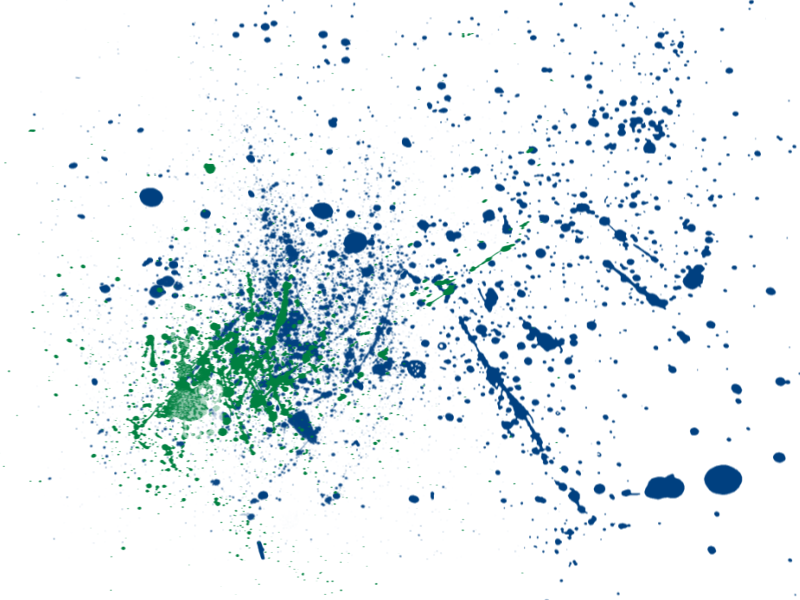
\includegraphics[width=\textwidth]{graphics/liquid_splatter_02.png}

\vfill


% 
% TUTORIAL : pll
%

\newpage
\section{Tutorial: Phase-Locked Loop}
\label{tutorial:pll}
This tutorial demonstrates the functionality of a carrier phase-locked
loop and introduces the {\tt iirfilt} object.
%
You will need on your local machine:
\begin{itemize}
\item the \liquid\ DSP libraries built and installed (see
      \S\ref{section:installation})
\item a text editor such as {\tt vim} \cite{vim:web}
\item a C compiler such as {\tt gcc} \cite{gcc:web}
\item a terminal
\end{itemize}
%
The problem statement and a brief theoretical description of
phase-locked loops is given in the next section.
A walk-through of the source code follows.

\subsection{Problem Statement}
\label{tutorial:pll:problem}
Wireless communications systems up-convert the data signal with
a high-frequency carrier before transmitting over the air.
This transmitted signal is orthogonal to other signals so long as
their bandwidths don't overlap and can be recovered at the receiver by
mixing it back down to baseband.
%This is accomplished by mixing the complex baseband signal...
%with a complex sinusoid, viz
%\[
%    s(t) = \Re\Bigl\{ m(t)\exp\{j\omega_ct\} \Bigr\}
%\]
Many digital communications systems modulate information in the phase of
the carrier requiring the receiver to demodulate the signal coherently
in order to recover the original data message.
In this regard the receiver must synchronize its carrier oscillator to
that of the transmitter.
To put it simply, the receiver must lock on to the phase of
transmitter's carrier.
One of the key advantages to performing signal processing in software is
that the radio can operate at complex baseband.
% TODO : expand on this
% (see \S\ref{section:complex_baseband}).

In this simulation, the received signal is simply a complex sinusoid
with an unknown initial carrier phase and frequency.
The carrier holds no information-bearing symbols and is simply a tone
whose frequency and phase represent the residual mismatch between the
transmitter and receiver.
The received signal $x$ at time step $k$ can be described as
%
\begin{equation}
\label{eqn:tutoral:pll:x}
    x_k = \exp\bigl\{ j(\theta + k\omega) \bigr\}
\end{equation}
%
where $j \triangleq \sqrt{-1}$ and
$\theta$ and $\omega$ represent the unknown initial carrier phase and
frequency offsets, respectively.
The receiver generates a complex sinusoid with a phase $\phi_k$ as the
phase difference between $x_k$ and $y_k$ and can be computed as
%
\begin{equation}
\label{eqn:tutoral:pll:y}
    y_k = \exp\bigl\{j\phi_k\bigr\}
\end{equation}
%
%which tries to minimize the difference between the phase of the ...
The phase error at time step $k$ is expressed as
%
\begin{equation}
\label{eqn:tutoral:pll:dphi}
    \Delta\phi_k = \arg\bigl\{ x_k y_k^* \bigr\}
\end{equation}
%
where $(^*)$ denotes complex conjugation.%
\footnote{
    Those who are savvy with communications techniques will
    appreciate that we are dealing in complex baseband and can easily
    compute the phase error estimate simply as the argument of the
    product of $x_k$ and $y_k$.
    Conventional PLLs which have operated strictly in the real domain
    multiply only the real components of $x_k$ and $y_k$ for a phase
    error estimate, assume that the loop filter rejects the
    high-frequency component, and make the approximation
    $\Delta\phi \approx \sin(\Delta\phi) = \sin(\phi-\hat{\phi})$
    for small phase errors.}
The goal of the receiver is to control $\phi_k$
(the phase of the output signal $y$ at time $k$)
to lock onto the input phase of $x$,
hence the name ``phase-locked loop.''
If the phase of the output sample $y_k$ is behind that of the input
($\Delta\phi > 0$) then $\phi$ needs to be advanced appropriately for
the next time step.
Conversely, if the phase of $y_k$ is ahead of the phase of $x_k$
($\Delta\phi < 0$) then the receiver need to retard $\phi$.

Without going into a great amount of detail, this control is
accomplished using a special filter within the loop.
This filter, known as a ``loop filter,'' is designed to reject
high-frequency noise and is described with the transfer function $H(z)$.
Specifically $H(z)$ is a 2$^{nd}$-order integrating low-pass recursive
filter with
a natural frequency $\omega_n$,
a damping factor $\zeta$, and
a loop gain $K$.
The natural frequency is the resonant frequency of $H(z)$ and for all
practical purposes is the filter's bandwidth.
Increasing $\omega_n$ permits the loop to track to the input signal
faster (reduces lock time), but also increases the amount of noise
passed through the loop.
Decreasing $\omega_n$ reduces this noise but also increases the loop's
acquisition time.
The damping factor $\zeta$ controls the stability of the filter and is
typically set to a value near $1/\sqrt{2} \approx 0.707$.
The loop gain $K$ is typically very large
(on the order of $1000$ or so).
For more detailed information on loop filter design the interested
reader is referred to \S\ref{module:nco:pll}.
% TODO : reference iirdes_pll_...() as well?

The estimated phase error $\Delta\phi_k$ is filtered using $H(z)$
resulting in an output phase estimate $\phi_{k+1}$
which is used for the subsequent output sample $y_{k+1}$ as
%
\begin{equation}
\label{eqn:tutoral:pll:y1}
    y_{k+1} = \exp\bigl\{ j\phi_{k+1} \bigr\}
\end{equation}
%
% ALGORITHM : phase-locked loop
\begin{algorithm}[H]
\caption{Phase-locked Loop Control}
\label{alg:tutorial:pll}
%\algsetup{linenosize=\footnotesize}
%\algsetup{linenodelimiter=:}
\algsetup{indent=2em}
\begin{algorithmic}[1]
\STATE $\vec{x} \leftarrow \{x_0,x_1,x_2,\ldots\}$    \COMMENT{input array}
\STATE $\hat{\phi}_0 \leftarrow 0$          \COMMENT{initial output phase}

\FOR{$k=0,\,1,\,2,\,\ldots$}
    \STATE $y_k \leftarrow \exp\bigl\{ j\hat{\phi}_k \bigr\}$ \COMMENT{compute output sample}
    \STATE $\Delta\phi_k \leftarrow \arg\bigl\{ x_k y_k^* \bigr\}$ \COMMENT{phase detector}
    \STATE $\hat{\phi}_{k+1} \leftarrow \text{filter}(\Delta\phi_k)$ \COMMENT{update output phase estimate}
\ENDFOR
\end{algorithmic}
\end{algorithm}
%
A summary of the algorithm is given in Algorithm~\ref{alg:tutorial:pll}.
In the next section we will create a simple C program to simulate a
phase-locked loop with \liquid.


\subsection{Setting up the Environment}
\label{tutorial:pll:environment}

For this tutorial and others, I assume that you are using the GNU
compiler collection ({\tt gcc}) for compiling source and linking objects
\cite{gcc:web},
and that you have a familiarity with the C (or C++) programming
language.
Create a new file {\tt pll.c} and open it with your favorite editor.
Include the headers {\tt stdio.h}, {\tt complex.h}, {\tt math.h}, and
{\tt liquid/liquid.h} and add the {\tt int main()} definition
so that your program looks like this:
%
\input{tutorials/pll_init_tutorial.c.tex}
%
Compile and link the program using {\tt gcc}:
%
\begin{Verbatim}[fontsize=\small]
    $ gcc -Wall -o pll -lm -lc -lliquid pll.c
\end{Verbatim}
%
The flag ``{\tt -Wall}'' tells the compiler to print all warnings
(unused and uninitialized variables, etc.),
``{\tt -o pll}'' specifies the name of the output program is
``{\tt pll}'', and
``{\tt -lm -lc -lliquid}'' tells the linker to link the binary against
the math, standard C, and \liquid\ DSP libraries, respectively.
Notice that the above command invokes both the compiler and the linker
collectively.
%While it is usually preferred to build an intermediate object...
%
If the compiler did not give any errors, the output executable {\tt pll}
is created which can be run as
\begin{Verbatim}[fontsize=\small]
    $ ./pll
\end{Verbatim}
%
and should simply print ``{\tt done.}'' to the screen.
You are now ready to add functionality to your program.

We will now edit the file to set up the basic simulation but without
controlling the phase of the output sinusoid.
As such the output won't track to the input resulting in a significant
amount of phase error.
This simulation will operate one sample at a time and is organized into
three sections.
First, set up the simulation parameters: the initial phase and frequency
offsets ({\tt float}),
and number of samples to run ({\tt unsigned int}).
Next, initialize the complex input and output variables
({\tt x} and {\tt y}) to zero,
as well as the state of the phase error ({\tt phase\_error})
and output phase ({\tt phi\_hat}) estimates.
Finally, set up the computational loop which generates the input and
output samples, computes the phase error between them, and then prints
the results to the screen.
%
Edit {\tt pll.c} to set up the basic simulation:
%
\input{tutorials/pll_basic_tutorial.c.tex}
%
% DISCECTION:
The variables {\tt x} and {\tt y} are of type {\tt float complex} which
contains both real and imaginary components of type {\tt float}.
%\footnote{
%    If, for some reason, you prefer C++ over C you could use the type
%    {\tt std::complex<float>} instead.
%    See \S\ref{xxx} for details.}
The function {\tt cexpf()} computes the complex exponential of its
argument which for a purely imaginary input $j\alpha$ is simply
$e^{j\alpha} = \cos\alpha + j\sin\alpha$.
% TODO : finish explanation

%
Compile and run the program as before.
The program should now output something like this:
%
\begin{Verbatim}[fontsize=\small]
      0 : phase =   0.00000000, error =   0.80000001
      1 : phase =   0.00000000, error =   0.81000000
      2 : phase =   0.00000000, error =   0.81999999
      3 : phase =   0.00000000, error =   0.82999998
      4 : phase =   0.00000000, error =   0.84000003
            ...
     35 : phase =   0.00000000, error =   1.14999998
     36 : phase =   0.00000000, error =   1.15999997
     37 : phase =   0.00000000, error =   1.17000008
     38 : phase =   0.00000000, error =   1.18000007
     39 : phase =   0.00000000, error =   1.19000006
    done.
\end{Verbatim}
%
Notice that because we aren't controlling the output phase yet
the error increases with the input phase.
In the next section we will design the loop filter to adjust the output
phase to lock onto the input signal given the phase error.

\subsection{Designing the Loop Filter}
\label{tutorial:pll:design}

Our program so far has not used any of the \liquid\ DSP libraries for
computation and has only relied on the standard C libraries for dealing
with complex math operations.
In this section we will introduce \liquid's {\tt iirfilt\_rrrf} object
to realize a recursive (infinite impulse response) filter with real
inputs, coefficients, and outputs.
Additionally we will use the function {\tt iirdes\_pll\_active\_lag()}
to design the coefficients for the PLL's filter,
specifically an ``active lag'' design.
While the explanation in this section is fairly long, relax!
We will only need to add about 15 lines of code to our program.
If you are eager to edit your program you may skip to
\S\ref{tutorial:pll:completed}.

Digital representations of infinite impulse response (IIR) filters have
two sets of coefficients: feedback and feedforward.
In the digital domain the transfer function is a ratio of the
polynomials in $z^{-1}$ where the feedforward coefficients
$\vec{b} = \{b_0, b_1, b_2, \ldots, b_{N-1}\}$
are in the numerator and the feedback coefficients
$\vec{a} = \{a_0, a_1, a_2, \ldots, a_{M-1}\}$
are in the denominator.
Specifically, the transfer function is
%
\begin{equation}
    H(z) =
        \frac{
            b_0 + b_1 z^{-1} + b_2 z^{-2} + \ldots + b_{N-1}z^{-(N-1)}
        }{
            a_0 + a_1 z^{-1} + a_2 z^{-2} + \ldots + a_{M-1}z^{-(M-1)}
        }
\end{equation}
%
This transfer function means that the output of the filter is the linear
combination of the $N$ previous filter inputs
%($\vec{x} = \{x_0, x_1, x_2, \ldots, x_{N-1}\}$)
($\vec{x}$)
and $M-1$ previous filter outputs
%($\vec{y} = \{y_0, y_1, y_2, \ldots, y_{M-1}\}$),
($\vec{y}$),
viz
%
\begin{eqnarray}
%    y_{k} =
%        \frac{1}{a_0}
%        \Bigl(
%            b_0 x_k &+& b_1 x_{k-1} + \cdots + b_{N-1} x_{k-N}\\
%                    &-& a_1 y_{k-1} - \cdots - a_{M-1} y_{k-M}
%        \Bigr)
    y[k] =
        \frac{1}{a_0}
        \Bigl(
            b_0 x[k] &+& b_1 x[k-1] + \cdots + b_{N-1} x[k-N]\\
                     &-& a_1 y[k-1] - \cdots - a_{M-1} y[k-M]
        \Bigr)
\end{eqnarray}
%
Typically the number of feedback and feedforward coefficients are equal
($M=N$), and the coefficients themselves are normalized so that $a_0=1$.

\liquid\ implements IIR filters with the {\tt iirfilt\_xxxt} family of
objects where ``{\tt xxxt}'' denotes the type definition
(see \S\ref{section:data_structures} for details).
In our example we will be using the {\tt iirfilt\_rrrf} object which
indicates that this is an IIR filter with real inputs, outputs, and
coefficients with precision of type {\tt float}.
The IIR filter objects in \liquid\ maintain their state
internally, storing the previous inputs and outputs in its internal
buffers.
Nearly every object in \liquid\ (filter or otherwise) has at least four
basic methods:
{\tt create()},
{\tt print()},
{\tt execute()}, and
{\tt destroy()}.
For our program we will need to create the filter object by passing to
it a vector of each the feedback and feedforward coefficients.
The infinite impulse response (IIR) filter we are designing is of order
two which means that $\vec{a}$ and $\vec{b}$ have three coefficients
each.

Generating the loop filter coefficients is fairly straightforward.
As stated before, the loop filter has parameters for
natural frequency $\omega_n$,
damping factor $\zeta$, and
loop gain $K$.
Furthermore the filter is 2$^{nd}$-order which means that it has three
coefficients each for $\vec{a}$ and $\vec{b}$.
\liquid\ provides a method for computing such a filter with the
{\tt iirdes\_pll\_active\_lag()} function
which accepts $\omega_n$, $\zeta$, and $K$ as inputs and generates the
coefficients in two output arrays.
The coefficients can be computed as follows:
%
\begin{Verbatim}[fontsize=\small]
    float wn = 0.1f;        // pll bandwidth
    float zeta = 0.707f;    // pll damping factor
    float K = 1000.0f;      // pll loop gain
    float b[3];             // feedforward coefficients array
    float a[3];             // feedback coefficients array
    iirdes_pll_active_lag(wn, zeta, K, b, a);
\end{Verbatim}
%
The life cycle of the IIR filter can be summarized as follows
%
\begin{Verbatim}[fontsize=\small]
    iirfilt_rrrf loopfilter = iirfilt_rrrf_create(b,3,a,3);
    float sample_in = 0.0f;
    float sample_out;
    {
        // repeat as necessary
        iirfilt_rrrf_execute(loopfilter, sample_in, &sample_out);
    }
    iirfilt_rrrf_destroy(loopfilter);
\end{Verbatim}
%
noting that the {\tt execute()} method can be repeated as many times as
necessary before the object is destroyed.

Using the code snippets above, modify your program to include the loop
filter to adjust the output signal's phase.
The input to the filter will be the {\tt phase\_error} variable, and its
output will be {\tt phi\_hat}.
Don't forget to destroy your filter object once the loop has finished
running.

\subsection{Final Program}
\label{tutorial:pll:completed}

The final program is listed below,
and a copy of the source is located in the {\tt doc/tutorials/}
subdirectory.
%
\input{tutorials/pll_tutorial.c.tex}
%
Compile the program as before, creating the executable ``{\tt pll}.''
Running the program should produce an output similar to this:
\begin{Verbatim}[fontsize=\small]
    iir filter [normal]:
      b :  0.32277358  0.07999840 -0.24277516
      a :  1.00000000 -1.99995995  0.99996001
      0 : phase =   0.25821885, error =   0.80000001
      1 : phase =   0.75852644, error =   0.55178112
      2 : phase =   1.12857747, error =   0.06147351
      3 : phase =   1.27319980, error =  -0.29857749
      4 : phase =   1.23918116, error =  -0.43319979
            ...
     35 : phase =   1.15999877, error =   0.00000751
     36 : phase =   1.17000139, error =   0.00000122
     37 : phase =   1.18000150, error =  -0.00000131
     38 : phase =   1.19000030, error =  -0.00000140
     39 : phase =   1.19999886, error =  -0.00000024
    done.
\end{Verbatim}
%
Notice that the phase error at the end of the output is very small.
The initial error (at $k=0$) is 0.8 which is the value of the
{\tt phase\_offset} parameter at the beginning of the program.
Notice also that the difference in phase of the last several samples
(i.e. the difference between the phase at steps {\tt 38} and {\tt 39})
is approximately 0.1 which is the initial frequency offset that was
given in the beginning.
Play around with the input parameters, particularly the frequency offset
and the phase-locked loop bandwidth.
Increasing the PLL bandwidth ({\tt wn}) should reduce the resulting
phase error more quickly.
The downside of having a PLL with a large bandwidth is that when the
input signal has been corrupted by noise then the phase error estimate
is also noisy.
In this tutorial no noise term was introduced. % TODO : explain more!


%% 
% TUTORIAL : modem
%

\newpage
\section{Tutorial: Digital Modem}
\label{tutorial:modem}

% 
% TUTORIAL : fec
%

\newpage
\section{Tutorial: Forward Error Correction}
\label{tutorial:fec}

This tutorial will demonstrate computation at the byte level
(raw message data) by
introducing the forward error-correction (FEC) coding module.
Please note that \liquid\ only provides some very basic FEC
capabilities including some Hamming block codes and repeat codes.
While these codes are very fast and enough to get started,
they are not very efficient and add a lot of redundancy without providing
a strong level of correcting capabilities.
\liquid\ will use the convolutional and Reed-Solomon codes described in
{\em libfec} \cite{libfec:web} if installed on your machine.
%While not a requirement...
% maybe in the future these can be imported into liquid-dsp...

\subsection{Problem Statement}
\label{tutorial:fec:problem}
Digital communications over a noisy channel can be unreliable,
resulting in errors at the receiver.
Forward error-correction (FEC) coding adds redundancy to the original
data message that allows for some errors to be corrected at the
receiver.
The error-correction capability of the code is dependent upon many
factors, but is usually improved by increasing the amount of redundancy
added to the message.
The drawback to adding a lot of redundancy is that the communications
rate is decreased as the link must be shared among the important data
information as well as the redundant bits.
The benefit, however, is that the receiver has a better chance of
correcting the errors without having to request a retransmission of the
message.
Volumes of research papers and books have been written about the
error-correction capabilities of certain FEC encoder/decoder pairs
(codecs) and their performance in a variety of environments.
While there is far too much information on the subject to discuss here,
it is important to note that \liquid\ implements a very small subset of
simple FEC codecs, including several Hamming and repeat codes.
If the {\em libfec} \cite{libfec:web} library is installed when \liquid\
is configured this list extends to convolutional and Reed-Solomon codes.

In this tutorial you will create a simple program that will generate a
message, encode it using a simple Hamming(7,4) code, corrupt the encoded
message by adding an error, and then try to correct the error with the
decoder.
%The length of the message, the encoding scheme, and the number of errors
%can be changed... xxx
% TODO : complete description


\subsection{Setting up the Environment}
\label{tutorial:fec:environment}

Create a new file {\tt fec.c} and open it with your favorite editor.
Include the headers {\tt stdio.h} and {\tt liquid/liquid.h}
and add the {\tt int main()} definition
so that your program looks like this:
%
\input{tutorials/fec_init_tutorial.c.tex}
%
Compile and link the program using {\tt gcc}:
%
\begin{Verbatim}[fontsize=\small]
    $ gcc -Wall -o fec -lm -lc -lliquid fec.c
\end{Verbatim}
%
The flag ``{\tt -Wall}'' tells the compiler to print all warnings
(unused and uninitialized variables, etc.),
``{\tt -o fec}'' specifies the name of the output program is
``{\tt fec}'', and
``{\tt -lm -lc -lliquid}'' tells the linker to link the binary against
the math, standard C, and \liquid\ DSP libraries, respectively.
Notice that the above command invokes both the compiler and the linker
collectively.
%While it is usually preferred to build an intermediate object...
%
If the compiler did not give any errors, the output executable {\tt fec}
is created which can be run as
%
\begin{Verbatim}[fontsize=\small]
    $ ./fec
\end{Verbatim}
%
and should simply print ``{\tt done.}'' to the screen.
You are now ready to add functionality to your program.

We will now edit the file to set up the basic simulation by generating a
message signal and counting errors as a result of channel effects.
The error-correction capabilities will be added in the next section.
First set up the simulation parameters: for now the only parameter will
be the length of the input message, denoted by the variable {\tt n}
({\tt unsigned int}) representing the number of bytes.
Initialize {\tt n} to 8 to reflect an original message of 8 bytes.
Create another {\tt unsigned int} variable {\tt k} which will represent
the length of the encoded message.
This length is equal to the original ({\tt n}) with the additional
redundancy.
For now set {\tt k} equal to {\tt n} as we are not adding FEC coding
until the next section.
This implies that without any redundancy, the receiver cannot correct
for any errors.

Message data in \liquid\ are represented as arrays of type
{\tt unsigned char}.
Allocate space for the original, encoded, and decoded messages as
{\tt msg\_org[n]},
{\tt msg\_enc[k]}, and
{\tt msg\_dec[n]}, respectively.
Initialize the original data message as desired.
For example, the elements in {\tt msg\_org} can contain
{\tt 0,1,2,...,n-1}.
Copy the contents of {\tt msg\_org} to {\tt msg\_enc}.
This effectively is a placeholder for forward error-correction which
will be discussed in the next section. % [reword]
Corrupt one of the bits in {\tt msg\_enc}
(e.g. {\tt msg\_enc[0] \verb|^|= 0x01;} will flip the least-significant bit in
the first byte of the {\tt msg\_enc} array),
and copy the results to {\tt msg\_dec}.
Print the encoded and decoded messages to the screen to verify that they
are not equal.
Without any error-correction capabilities, the receiver should see a
message different than the original because of the corrupted bit.
Count the number of bit differences between the original and decoded
messages.
\liquid\ provides a convenient interface for doing this and can be
invoked as
%
\begin{Verbatim}[fontsize=\small]
    unsigned int num_bit_errors = count_bit_errors_array(msg_org,
                                                         msg_dec,
                                                         n);
\end{Verbatim}
%
Print this number to the screen.
Your program should look similar to this:
%
\input{tutorials/fec_basic_tutorial.c.tex}
%
Compile the program as before, creating the executable ``{\tt fec}.''
Running the program should produce an output similar to this:
%
\begin{Verbatim}[fontsize=\small]
    original message:  [  8]  00 01 02 03 04 05 06 07
    decoded message:   [  8]  01 01 02 03 04 05 06 07
    number of bit errors received:      1 /  64
\end{Verbatim}
%
Notice that the decoded message differs from the original and that the
number of received errors is nonzero.


%
% SUBSECTION : creating the encoder
%
\subsection{Creating the Encoder/Decoder}
\label{tutorial:fec:codec}
% talking points
%   * Hamming(7,4) is a weak code
%   * liquid abstracts from gritty details
%   * 
So far our program doesn't use any \liquid\ interfaces (except for the
function used to count bit errors).
The FEC module in \liquid\ provides a simple interface for adding
forward error-correction capabilities to your project.
The {\tt fec} object abstracts from the gritty details behind the bit
manipulation (packing/unpacking of bytes, appending tail bits, etc.)
of error-correction structures.
As an example, convolutional codes observe bits one at a time while
Reed-Solomon codes operate on entire blocks of bits.
%If you wanted to switch between codes you would need to...
The {\tt fec} object in \liquid\ conveniently abstracts from the
organization of the codec and takes care of this overhead internally.
This allows seamless integration of different codecs with one simple
interface.
%
As with the {\tt iirfilt\_rrrf} object in the phase-locked loop tutorial
(\S\ref{tutorial:pll})
the {\tt fec} object has methods
{\tt create()},
{\tt print()}, and
{\tt destroy()}.
Nearly every object in \liquid\ has these methods;
however the {\tt fec} object replaces {\tt execute()} with
{\tt encode()} and {\tt decode()} as the
same object instance can be used for both encoding and decoding.
The {\tt fec\_create()} method accepts two arguments, although the
second one is basically ignored.
The first argument is an enumeration of the type of codec that you wish
to use.

To begin, create a new {\tt fec} object of type {\tt LIQUID\_FEC\_HAMMING74}
(the second argument can simply be {\tt NULL})
which creates a Hamming(7,4) code:
%
\begin{Verbatim}[fontsize=\small]
    fec q = fec_create(LIQUID_FEC_HAMMING74, NULL);
\end{Verbatim}
%
Details of the available codes in \liquid\ can be found in
\S\ref{module:fec}.
This codec nominally accepts 4 bits, appends 3 parity bits, and can
detect and correct up to one of these seven transmitted bits.
The Hamming(7,4) code is not particularly strong for its rate;
however it is computationally efficient and has been studied extensively
in coding theory.
The interface provided by \liquid\ conveniently abstracts from the
process of managing 8-bit data symbols (bytes), converting to 4-bit
input symbols, encoding to 7-bit output symbols, and then re-packing
into 8-bit output bytes.
This is consistent with {\em any} forward error-correction code in
\liquid;
as the user, you simply see data bytes in and data bytes out.
The length of the output sequence can be computed using the method
%
\begin{Verbatim}[fontsize=\small]
    unsigned int k = fec_get_enc_msg_length(LIQUID_FEC_HAMMING74, n);
\end{Verbatim}
%
where {\tt n} represents the number of uncoded input bytes
and   {\tt k} represents the number of encoded output bytes.
This value should be used to appropriately allocate enough memory for
the encoded message.
%
Encoding the data message is as simple as invoking
%
\begin{Verbatim}[fontsize=\small]
    fec_encode(q, n, msg_org, msg_enc);
\end{Verbatim}
%
which uses our newly-created {\tt fec} object {\tt q} to encode {\tt n}
input bytes in the array {\tt msg\_org} and store the result in the
output array {\tt msg\_enc}.
The interface for decoding is nearly identical:
%
\begin{Verbatim}[fontsize=\small]
    fec_decode(q, n, msg_enc, msg_dec);
\end{Verbatim}
%
Notice that the second argument again represents the number of
{\em uncoded} data bytes ({\tt n}).
Don't forget to destroy the object once you are finished:
%
\begin{Verbatim}[fontsize=\small]
    fec_destroy(q);
\end{Verbatim}
%


\subsection{Final Program}
\label{tutorial:fec:completed}

The final program is listed below,
and a copy of the source is located in the {\tt doc/tutorials/}
subdirectory.
%
\input{tutorials/fec_tutorial.c.tex}
%
The output should look like this:
%
\begin{Verbatim}[fontsize=\small]
    fec: Hamming(7,4) [rate: 0.571]
    original message:  [  8]  00 01 02 03 04 05 06 07
    decoded message:   [  8]  00 01 02 03 04 05 06 07
    number of bit errors received:      0 /  64
    done.
\end{Verbatim}
%
Notice that the decoded message matches that of the original message,
even though an error was introduced at the receiver.
As discussed above, the Hamming(7,4) code is not particularly strong;
if too many bits in the encoded message are corrupted then the decoder
will be unable to correct them.
Play around with changing the length of the original data message,
the encoding scheme, and the number of errors introduced.

For a more detailed program, see {\tt examples/fec\_example.c} in the
main \liquid\ directory.
\S\ref{module:fec} describes \liquid's FEC module in detail.
Additionally, the {\tt packetizer} object extends the simplicity of the
{\tt fec} object by adding a cyclic redundancy check and two layers of
forward error-correction and interleaving, all of which can be
reconfigured as desired.
See \S\ref{module:framing:packetizer} and
{\tt examples/packetizer\_example.c} for a detailed example program
on how to use the {\tt packetizer} object.


% 
% TUTORIAL : framing
%

\newpage
\section{Tutorial: Framing}
\label{tutorial:framing}

In the previous tutorials we have created only the basic building blocks
for wireless communication.
This tutorial puts them all together by introducing a very simple
framing structure for sending and receiving data over a wireless link.
In this context ``framing'' refers to the encapsulation of data into a
modulated time series at complex baseband to be transmitted over a
wireless link.
Conversely, ``packets'' refer to packing raw message data bytes with
forward error-correction and data validity check redundancy.


%
% SUBSECTION : problem statement
%
\subsection{Problem Statement}
\label{tutorial:framing:problem}

%To properly convey information over a wireless link...
For this tutorial we will be using the {\tt framegen64} and
{\tt framesync64} objects in \liquid.
As you might have guessed {\tt framegen64} is the frame generator object
on the transmit side of the link
and {\tt framesync64} is the frame synchronizer on the receive side.
%
Together these objects realize a
a very simple frame which encapsulates a 12-byte header and 64-byte
payload within a frame consisting of 640 symbols at complex baseband.
Conveniently the frame generator interpolates these symbols with a
matched filter to produce a 1280-sample frame at complex baseband,
ready to be up-converted and transmitted over the air.
This frame has a nominal spectral efficiency of 0.8 bits/second/Hz
(512 bits from 64 payload bytes assembled in 640 symbols).%
\footnote{
    For simplicity this computation of spectral efficiency
    neglects any excess bandwidth of the pulse-shaping filter.}
This means that if you transmit with a symbol rate of 10kHz you should
expect to see a throughput of 8kbps if all the frames are properly
decoded.
On the receiving side,
raw samples at complex baseband are streamed to an instance of
the frame synchronizer which picks out frames and invokes a user-defined
callback function.
The synchronizer corrects for gain, carrier, and sample timing offsets
(channel impairments) in the complex baseband samples with a minimal
amount of pre-processing required by the user.
%
To help with synchronization, the frame includes a special preamble
which can be seen in the figure below.\\
%
% FIGURE: framing:structure
\includegraphics[width=\textwidth]{figures.pgf/framing_structure}\\
%
After up-conversion (mixing up to a carrier frequency) the frame is
transmitted over the link where the receiver mixes the signal back down to
complex baseband.
The received signal will be attenuated and noisy and typically degrades
with distance between the two radios.
Also, because receiver's oscillators run independent of the
transmitter's,
this received signal will have other impairments such as carrier
and timing offsets.
In our program we will be operating at complex baseband and will add the
channel impairments artificially.

The frame synchronizer's purpose is to correct for all of these
impairments (within limitations, of course) and attempt to detect the
frame and decode its data.
The framing preamble assists the synchronizer by introducing special
phasing sequences before any information-bearing symbols which aids in
correcting for carrier and timing offsets.
Without going into great detail, these sequences significantly increase
the probability of frame detection and decoding while adding a minimal
amount of overhead to the frame;
a small price to pay for increased data reliability!


%
% SUBSECTION : 
%
\subsection{Setting up the Environment}
\label{tutorial:framing:environment}

As with the other tutorials I assume that you are using {\tt gcc} to
compile your programs and link to appropriate libraries.
Create a new file {\tt framing.c} and include the headers
{\tt stdio.h},
{\tt stdlib.h},
{\tt math.h},
{\tt complex.h}, and
{\tt liquid/liquid.h}.
Add the {\tt int main()} definition so that your program looks like
this:
%
\input{tutorials/framing_init_tutorial.c.tex}
%
Compile and link the program using {\tt gcc}:
%
\begin{Verbatim}[fontsize=\small]
    $ gcc -Wall -o framing -lm -lc -lliquid framing.c
\end{Verbatim}
%
The flag ``{\tt -Wall}'' tells the compiler to print all warnings
(unused and uninitialized variables, etc.),
``{\tt -o framing}'' specifies the name of the output program is
``{\tt framing}'', and
``{\tt -lm -lc -lliquid}'' tells the linker to link the binary against
the math, standard C, and \liquid\ DSP libraries, respectively.
Notice that the above command invokes both the compiler and the linker
collectively.
%While it is usually preferred to build an intermediate object...
%
If the compiler did not give any errors, the output executable
{\tt framing} is created which can be run as
%
\begin{Verbatim}[fontsize=\small]
    $ ./framing
\end{Verbatim}
%
and should simply print ``{\tt done.}'' to the screen.
You are now ready to add functionality to your program.



%
% SUBSECTION : frame generator
%
\subsection{Creating the Frame Generator}
\label{tutorial:framing:framegen}
% talking points
%   * components to a frame
%       * header
%       * payload
%       * etc.
%   * options (m, beta)
The particular framing structure we will be using accepts a 12-byte
header and a 64-byte payload and assembles them into a frame
consisting of 1280 samples.
These sizes are fixed and cannot be adjusted for this framing
structure.%
\footnote{
    Alternatively, the {\tt flexframegen} and {\tt flexframesync}
    objects implement a dynamic framing structure which has many more
    options than the {\tt framegen64} and {\tt framesync64} objects.
    See \S\ref{module:framing} for details.}
The purpose of the header is to conveniently allow the user a separate
control channel to be packaged with the payload.
For example, if your application is to send a file using multiple
frames, the header can include an identification number to indicate
where in the file it should be written.
Another application of the header is to include a destination node
identifier for use in packet routing for ad hoc networks.
Both the header and payload are assembled with a 16-bit cyclic
redundancy check (CRC) to validate the integrity of the received data
and encoded using the Hamming(12,8) code for error correction.
(see \S\ref{module:fec} for more information on error detection
and correction capabilities in \liquid).
The encoded header and payload are modulated with QPSK and encapsulated
with a BPSK preamble.
Finally, the resulting symbols are interpolated using a square-root
Nyquist matched filter at a rate of 2 samples per symbol.
This entire process is handled internally so that as a user the only
thing you will need to do is call one function.

The {\tt framegen64} object can be generated with the
{\tt framegen64\_create()} method which accepts two arguments:
an {\tt unsigned int} and a {\tt float}
representing the matched filter's length (in symbols) and
excess bandwidth factor, respectively.
To begin, create a frame generator having a square-root Nyquist filter
with a delay of 3 and an excess bandwidth factor of 0.7 as
%
\begin{Verbatim}[fontsize=\small]
    framegen64 fg = framegen64_create(3, 0.7);
\end{Verbatim}
%
As with all structures in \liquid\ you will need to invoke the
corresponding {\tt destroy()} method when you are finished with the
object.
Now allocate memory for the header and payload data arrays,
remembering that they have lengths 12 and 64, respectively.
Raw ``message'' data are stored as arrays of type {\tt unsigned char} in
\liquid.
%
\begin{Verbatim}[fontsize=\small]
    unsigned char header[12];
    unsigned char payload[64];
\end{Verbatim}
%
Finally you will need to create a buffer for storing the frame samples.
For this framing structure you will need to allocate 1280 samples of
type {\tt float complex}, viz
%
\begin{Verbatim}[fontsize=\small]
    float complex y[1280];
\end{Verbatim}
%
Initialize the header and payload arrays with whatever values you wish.
All that is needed to generate a frame is to invoke the frame
generator's {\tt execute()} method:
%
\begin{Verbatim}[fontsize=\small]
    framegen64_execute(fg, header, payload, y);
\end{Verbatim}
%
That's it!
This completely assembles the frame complete with interpolation and is
ready for up-conversion and transmission.
To generate another frame simply write whatever data you wish to the
header and payload buffers, and invoke the {\tt framegen64\_execute()}
method again as done above.
If you wish, print the first few samples of the generated frame to the
screen (you will need to separate the {\em real} and {\em imaginary}
components of each sample).
%
\begin{Verbatim}[fontsize=\small]
    for (i=0; i<30; i++)
        printf("%3u : %12.8f + j*%12.8f\n", i, crealf(y[i]), cimagf(y[i]));
\end{Verbatim}
%
Your program should now look similar to this:
%
\input{tutorials/framing_basic_tutorial.c.tex}
%
Compile the program as before, creating the executable
``{\tt framing}.''
Running the program should produce an output similar to this:
%
\begin{Verbatim}[fontsize=\small]
framegen64 [m=3, beta=0.70]:
    ramp/up symbols     :   16
    phasing symbols     :   64
    p/n symbols         :   64
    header symbols      :   84
    payload symbols     :   396
    payload symbols     :   396
    ramp\down symbols   :   16
    total symbols       :   640
  0 :   0.00000000 + j*  0.00000000
  1 :   0.00000000 + j*  0.00000000
  2 :  -0.00011255 + j*  0.00000000
  3 :   0.00014416 + j*  0.00000000
  4 :   0.00040660 + j*  0.00000000
        ...
 25 :   0.04375378 + j*  0.00000000
 26 :   0.97077769 + j*  0.00000000
 27 :  -0.04032370 + j*  0.00000000
 28 :  -1.09209442 + j*  0.00000000
 29 :   0.03534408 + j*  0.00000000
done.
\end{Verbatim}
%
You might notice that the {\em imaginary} component of the samples in
the beginning of the frame are zero.
This is because the preamble of the frame is BPSK which has no imaginary
component at complex baseband.

%
% SUBSECTION : frame synchronizer
%
\subsection{Creating the Frame Synchronizer}
\label{tutorial:framing:framesync}
% talking points
%   * what framesync actually does
%       * gain control
%       * frame synchronization
%       * symbol timing recovery
%       * carrier phase recovery
%       * matched filtering
%       * demodulation
%       * frame decoding
%   * _coherent_ demodulation (eliminate phase ambiguity)
%   * what is a callback function?

As stated earlier the frame synchronizer's purpose is to detect the
presence of a frame, correct for the channel impairments, decode the
data, and pass it back to the user.
In our program we will simply pass to the frame synchronizer the samples
we generated in the previous section with the frame generator.
%In real system, however, the receiver does not know when the beginning
%of the frame is and so...
Furthermore, the hardware interface might pass the baseband samples to
the synchronizer in blocks much smaller than the length of a frame
(512 samples, for instance)
or even blocks much {\em larger} than the length of a frame
(4096 samples, for instance).
How does the synchronizer relay the decoded data back to the program
without missing any frames?
The answer is through the use of a callback function.

What is a callback function?
Put quite simply, a callback function is a function pointer
(a designated address in memory)
that is invoked during a certain event.
For this example the callback function given to the {\tt framesync64}
synchronizer object when the object is created
and is invoked whenever the synchronizer finds a frame.
This happens irrespective of the size of the blocks passed to the
synchronizer.
If you pass it a block of data samples containing four frames|several
thousand samples|then the callback will be invoked four times
(assuming that channel impairments haven't corrupted the frame beyond
the point of recovery).
You can even pass the synchronizer one sample at a time if you wish.

The {\tt framesync64} object can be generated with the
{\tt framesync64\_create()} method which accepts three pointers as
arguments:
%
\begin{Verbatim}[fontsize=\small]
    framesync64 framesync64_create(framesyncprops_s *   _props,
                                   framesync64_callback _callback,
                                   void *               _userdata);
\end{Verbatim}
%
%Here is a description of...
%
\begin{description}
\item[{\tt \_props}]
    is a construct that defines the specific properties of the frame
    synchronizer.
    This includes loop bandwidths for carrier, timing, and gain
    recovery, as well as squelch and equalizer control.
    You may pass the value {\tt NULL} to use the default parameters
    (recommended for now).
\item[{\tt \_callback}]
    is a pointer to your callback function which will be invoked each
    time a frame is found and decoded.
\item[{\tt \_userdata}]
    is a {\tt void} pointer that is passed to the callback function each
    time it is invoked.
    This allows you to easily pass data from the callback function.
    Set to {\tt NULL} if you don't wish to use this.
\end{description}
%
The {\tt framesync64} object has a callback function which has six
arguments and looks like this:
%
\begin{Verbatim}[fontsize=\small]
    int framesync64_callback(unsigned char *  _header,
                             int              _header_valid,
                             unsigned char *  _payload,
                             int              _payload_valid,
                             framesyncstats_s _stats,
                             void *           _userdata);
\end{Verbatim}
%
The callback is typically defined to be {\tt static} and is passed to
the instance of {\tt framesync64} object when it is created.
%
\begin{description}
\item[{\tt \_header}]
    is a pointer to the 12 bytes of decoded header data.
    This pointer is not static and cannot be used after returning from
    the callback function.
    This means that it needs to be copied locally for you to retain the
    data.
\item[{\tt \_header\_valid}]
    is simply a flag to indicate if the header passed its cyclic
    redundancy check
    (``{\tt 0}'' means invalid, ``{\tt 1}'' means valid).
    If the check fails then the header data most likely has been
    corrupted beyond the point that the internal error-correction code
    can recover; proceed with caution!
\item[{\tt \_payload}]
    is a pointer to the 64 bytes of decoded payload data.
    Like the header,
    this pointer is not static and cannot be used after returning from
    the callback function.
    Again, this means that it needs to be copied locally for you to retain the
    data.
\item[{\tt \_payload\_valid}]
    is simply a flag to indicate if the payload passed its cyclic
    redundancy check
    (``{\tt 0}'' means invalid, ``{\tt 1}'' means valid).
    As with the header,
    if this flag is zero then the payload most likely has errors in it.
    Some applications are error tolerant and so it is possible that the
    payload data are still useful.
    Typically, though, the payload should be discarded and a
    re-transmission request should be issued.
\item[{\tt \_stats}]
    is a synchronizer statistics construct that indicates some useful
    PHY information to the user.
    We will ignore this information in our program, but it can be quite
    useful for certain applications.
    For more information on the {\tt framesyncstats\_s} structure, see
    \S\ref{module:framing:framesyncstats_s}.
\item[{\tt \_userdata}]
    Remember that {\tt void} pointer you passed to the {\tt create()}
    method?
    That pointer is passed to the callback and can represent just about
    anything.
    Typically it points to another structure and is the method
    by which the decoded header and payload data are returned to the
    program outside of the callback.
\end{description}
%
This can seem a bit overwhelming at first, but relax!
The next version of our program will only add about 20 lines of code.


%
% SUBSECTION : 
%
\subsection{Putting it All Together}
\label{tutorial:framing:xxx}
% talking points

First create your callback function at the beginning of the file, just
before the {\tt int main()} definition;
you may give it whatever name you like (e.g. {\tt mycallback()}).
For now ignore all the function inputs and just print a message to the
screen that indicates that the callback has been invoked,
and return the integer zero ({\tt 0}).
This return value for the callback function should always be zero
and is reserved for future development.
Within your {\tt main()} definition, create an instance of
{\tt framesync64} using the {\tt framesync64\_create()} method,
passing it a {\tt NULL} for the first and third arguments
(the properties and userdata constructs)
and the name of your callback function as the second argument.
Print the newly created synchronizer object to the screen if you like:
%
\begin{Verbatim}[fontsize=\small]
    framesync64 fs = framesync64_create(NULL,
                                        mycallback,
                                        NULL);
    framesync64_print(fs);
\end{Verbatim}
%
After your line that generates the frame samples
(``{\tt framegen64\_execute(fg, header, payload, y);}'')
invoke the synchronizer's {\tt execute()} method,
passing to it the frame synchronizer object you just created ({\tt fs}),
the pointer to the array of frame symbols ({\tt y}),
and the length of the array (1280):
%
\begin{Verbatim}[fontsize=\small]
    framesync64_execute(fs, y, 1280);
\end{Verbatim}
%
Finally, destroy the frame synchronizer object along with the frame
generator at the end of the file.
That's it!
Your program should look something like this:
%
\input{tutorials/framing_intermediate_tutorial.c.tex}
%
Compile and run your program as before and verify that your callback
function was indeed invoked.
Your output should look something like this:
%
\begin{Verbatim}[fontsize=\small]
    framegen64 [m=3, beta=0.70]:
        ramp/up symbols     :   16
        phasing symbols     :   64
        ...
    framesync64:
        agc signal min/max  :   -40.0 dB /  30.0dB
        agc b/w open/closed :   1.00e-03 / 1.00e-05
        sym b/w open/closed :   8.00e-02 / 5.00e-02
        pll b/w open/closed :   2.00e-02 / 5.00e-03
        samples/symbol      :   2
        filter length       :   3
        num filters (ppfb)  :   32
        filter excess b/w   :   0.7000
        squelch             :   disabled
        auto-squelch        :   disabled
        squelch threshold   :   -35.00 dB
        ----
        p/n sequence len    :   64
        payload len         :   64 bytes
    ***** callback invoked!
    done.
\end{Verbatim}
%
% ignore any lines pertaining to
%   framesync64/debug: results written to framesync64_internal_debug.m
As you can see, the {\tt framesync64} object has a long list of
modifiable properties pertaining to synchronization;
the default values provide a good initial set for a wide range of
channel conditions.
Duplicate the line of your code that executes the frame synchronizer.
Recompile and run your code again.
You should see the ``{\tt ***** callback invoked!}'' printed twice.

Your program has only demonstrated the basic functionality of the frame
generator and synchronizer under ideal conditions:
no noise, carrier offsets, etc.
The next section will add some channel impairments to stress the
synchronizer's ability to decode the frame.


%
% SUBSECTION : 
%
\subsection{Final Program}
\label{tutorial:framing:completed}

In this last section we will add some channel impairments to the frame
after it is generated and before it is received.
This will simulate non-ideal channel conditions.
Specifically we will introduce carrier frequency and phase offsets,
channel attenuation, and noise.
We will also add a frame counter and pass it through the {\em userdata}
construct in the frame synchronizer's {\tt create()} method to be passed
to the callback function when a frame is found.
Finally, the program will split the frame into pieces to emulate
non-contiguous data partitioning at the receiver.

To begin, add the following parameters to the beginning of your
{\tt main()} definition with the other options:
%
\begin{Verbatim}[fontsize=\small]
    unsigned int frame_counter = 0; // userdata passed to callback
    float phase_offset=0.3f;        // carrier phase offset
    float frequency_offset=0.02f;   // carrier frequency offset
    float SNRdB = 10.0f;            // signal-to-noise ratio [dB]
    float noise_floor = -40.0f;     // noise floor [dB]
\end{Verbatim}
%
The {\tt frame\_counter} variable is simply a number we will pass to the
callback function to demonstrate the functionality of the userdata
construct.
Make sure to initialize {\tt frame\_counter} to zero.
%
If you completed the tutorial on phase-locked loop design you might
recognize the {\tt phase\_offset} and {\tt frequency\_offset} variables;
these will be used in the same way to represent a carrier mismatch
between the transmitter and receiver.
%
The channel gain and noise parameters are a bit trickier and are set up
by the next two lines.
Typically the noise power is a fixed value in a receiver;
what changes is the received power based on the transmitter's power and
the gain of the channel;
however because theory dictates that the performance of a link is
governed by the ratio of signal power to noise power,
SNR is a more useful than defining signal amplitude and noise variance
independently.
The {\tt SNRdB} and {\tt noise\_floor} parameters fully describe the
channel in this regard.
The noise standard deviation and channel gain may be derived from these
values as follows:
%
\begin{Verbatim}[fontsize=\small]
    float nstd  = powf(10.0f, noise_floor/20.0f);
    float gamma = powf(10.0f, (SNRdB+noise_floor)/20.0f);
\end{Verbatim}
%
Add to your program
(after the {\tt framegen64\_execute()} line)
a loop that modifies each sample of the generated frame by introducing
the channel impairments.
%
\[
    y_i \leftarrow \gamma y_i e^{j(\theta + i\omega)} + \sigma n
\]
%
where
$y_i$ is the frame sample at index $i$ ({\tt y[i]}),
$\gamma$ is the channel gain defined above ({\tt gamma}),
$\theta$ is the carrier phase offset ({\tt phase\_offset}),
$\omega$ is the carrier frequency offset ({\tt frequency\_offset}),
$\sigma$ is the noise standard deviation defined above ({\tt nstd}), and
$n$ is a circular Gauss random variable.
\liquid\ provides the {\tt randnf()} methods to
generate real random numbers with a Gauss distribution;
a circular Gauss random variable can be generated from two regular Gauss
random variables $n_i$ and $n_q$ as $n = (n_i + jn_q)/\sqrt{2}$.
%
\begin{Verbatim}[fontsize=\small]
    y[i] *= gamma;
    y[i] *= cexpf(_Complex_I*(phase_offset + i*frequency_offset));
    y[i] += nstd * (randnf() + _Complex_I*randnf())*0.7071;
\end{Verbatim}
%
Check the program listed below if you need help.

Now modify the program to incorporate the frame counter.
First modify the piece of code where the frame synchronizer is created:
replace the last argument (initially set to {\tt NULL}) with the address
of our {\tt frame\_counter} variable.
For posterity's sake, this address will need to be type cast to
{\tt void*} (a void pointer) to prevent the compiler from complaining.
In your callback function you will reverse this process:
create a new variable of type {\tt unsigned int*}
(a pointer to an unsigned integer)
and assign it the {\tt \_userdata} argument type cast to
{\tt unsigned int*}.
Now de-reference this variable and increment its value.
Finally print its value near the end of the {\tt main()} definition to
ensure it is being properly incremented.
Again, check the program below for assistance.

The last task we will do is push one sample at a time to the frame
synchronizer rather than the entire frame block to emulate
non-contiguous sample streaming.
To do this, simply remove the line that calls
{\tt framesync64\_execute()} on the entire frame
and replace it with a loop that calls the same function but with one
sample at a time.

The final program is listed below,
and a copy of the source is located in the {\tt doc/tutorials/}
subdirectory.
%
\input{tutorials/framing_tutorial.c.tex}
%
Compile and run the program as before.
The output of your program should look something like this:
%
\begin{Verbatim}[fontsize=\small]
    framegen64 [m=3, beta=0.70]:
        ramp/up symbols     :   16
        phasing symbols     :   64
        ...
    framesync64:
        agc signal min/max  :   -40.0 dB /  30.0dB
        agc b/w open/closed :   1.00e-03 / 1.00e-05
        ...
    ***** callback invoked!
      header (valid)
      payload (valid)
    received 1 frames
    done.
\end{Verbatim}
%
% extra credit
Play around with the initial options, particularly those pertaining to
the channel impairments.
Under what circumstances does the synchronizer miss the frame?
For example, what is the minimum SNR level that is required to reliably
receive a frame?
the maximum carrier frequency offset?

% additional notes:
The ``random'' noise generated by the program will be seeded to the same
value every time the program is run.
A new seed can be initialized on the system's time (e.g. time of day) to
help generate new instances of random numbers each time the program is
run.
To do so, include the {\tt <time.h>} header to the top of your file and
add the following line to the beginning of your program's {\tt main()}
definition:
%
\begin{Verbatim}[fontsize=\small]
    srand(time(NULL));
\end{Verbatim}
%
This will ensure a unique simulation is run each time the program is
executed.
For a more detailed program, see {\tt examples/framesync64\_example.c}
in the main \liquid\ directory.
\S\ref{module:framing} describes \liquid's framing module in
detail.


% flexframe
While the framing structure described in this section provides a simple
interface for transmitting and receiving data over a channel,
its functionality is limited and isn't particularly spectrally
efficient.
\liquid\ provides a more robust framing structure which allows the use
of any linear modulation scheme, two layers of forward error-correction
coding, and a variable preamble and payload length.
These properties can be reconfigured for each frame to allow fast
adaptation to quickly varying channel conditions.
Furthermore, the frame synchronizer on the receiver automatically
reconfigures itself for each frame it detects to allow as simple an
interface possible.
The frame generator and synchronizer objects are denoted
{\tt flexframegen} and
{\tt flexframesync},
respectively,
and are described in \S\ref{module:framing}.
A detailed example program {\tt examples/flexframesync\_example.c}
is available in the main \liquid\ directory.


% 
% TUTORIAL : ofdmflexframe
%

\newpage
\section{Tutorial: OFDM Framing}
\label{tutorial:ofdmflexframe}

In the previous tutorials we have created only the basic building blocks
for wireless communication.
We have also used the basic {\tt framegen64} and {\tt framesync64}
objects to transmit and receive simple framing data.
This tutorial extends the work on the previous tutorials by introducing
a flexible framing structure that uses a parallel data transmission
scheme that permits arbitrary parametrization
(modulation, forward error-correction, payload length, etc.)
with minimal reconfiguration at the receiver.


%
% SUBSECTION : problem statement
%
\subsection{Problem Statement}
\label{tutorial:ofdmflexframe:problem}
% talking points:
%   * what is OFDM (briefly)
%   * the benefits of OFDM (briefly)
%   * current standards using OFDM
The framing tutorial (\S\ref{tutorial:framing}) loaded data serially
onto a single carrier.
Another option is to load data onto many carriers in parallel;
however it is desirable to do so such that bandwidth isn't wasted.
By allowing the ``subcarriers'' to overlap in frequency,
the system approaches the theoretical maximum capacity of the channel.
Several multiplexing schemes are possible,
but by far the most common is generically known as
orthogonal frequency divisional multiplexing (OFDM)
which uses a square temporal pulse shaping filter for each subcarrier,
separated in frequency by the inverse of the symbol rate.
This conveniently allows data to be loaded into the input of an inverse
discrete Fourier transform (DFT) at the transmitter and
(once time and carrier synchronized)
de-multiplexed with a regular DFT at the receiver.
For computational efficiency the DFT may be implemented with a fast
Fourier transform (FFT) which is mathematically equivalent
but considerably faster.
Furthermore, because of the cyclic nature of the DFT a certain portion
(usually on the order of 10\%)
of the tail of the generated symbol may be copied to its head before
transmitting;
this is known as the {\em cyclic prefix} which can eliminate
inter-symbol interference in the presence of multi-path channel
environments.
Carrier frequency and symbol timing offsets can be tracked and corrected
by inserting known {\em pilot subcarriers} in the signal at the
transmitter;
because the receiver knows the pilot symbols it can make an accurate
estimate of the channel conditions for each OFDM symbol.
%
% TODO : insert figures
%
As an example, the well-known Wi-Fi 802.11a standard uses OFDM with
64 subcarriers
(52 for data, 4 pilots, and 8 disabled for guard bands)
and a 16-sample cyclic prefix.
%
%For more details of OFDM I refer the interested reader to the following
%excellent publications...

In this tutorial we will create a simple pair of OFDM framing objects;
the generator ({\tt ofdmflexframegen}),
like the {\tt framegen64} object,
has a simple interface that accepts raw data in, frame samples out.
The synchronizer ({\tt ofdmflexframesync}),
like the {\tt framesync64} object,
accepts samples and invokes a callback function for each frame that it
detects,
compensating for sample timing and carrier offsets and multi-path
channels.
The framing objects can be created with nearly any even-length transform
(number of subcarriers),
cyclic prefix, and arbitrary null/pilot/data subcarrier allocation.%
\footnote{While nearly any arbitrary configuration is supported, the
          performance of synchronization is greatly dependent upon the
          choice of the number, type, and allocation of subcarriers.
          % See \S\ref{xxx} for a recommendation...
          }
Furthermore, the OFDM frame generator permits many different parameters
(e.g. modulation/coding schemes, payload length)
which are detected automatically at the receiver without any work on
your part.


%
% SUBSECTION : 
%
\subsection{Setting up the Environment}
\label{tutorial:ofdmflexframe:environment}

As with the other tutorials I assume that you are using {\tt gcc} to
compile your programs and link to appropriate libraries.
Create a new file {\tt ofdmflexframe.c} and include the headers
{\tt stdio.h},
{\tt stdlib.h},
{\tt math.h},
{\tt complex.h}, and
{\tt liquid/liquid.h}.
Add the {\tt int main()} definition so that your program looks like
this:
%
\input{tutorials/ofdmflexframe_init_tutorial.c.tex}
%
Compile and link the program using {\tt gcc}:
%
\begin{Verbatim}[fontsize=\small]
    $ gcc -Wall -o ofdmflexframe -lm -lc -lliquid ofdmflexframe.c
\end{Verbatim}
%
The flag ``{\tt -Wall}'' tells the compiler to print all warnings
(unused and uninitialized variables, etc.),
``{\tt -o ofdmflexframe}'' specifies the name of the output program is
``{\tt ofdmflexframe}'', and
``{\tt -lm -lc -lliquid}'' tells the linker to link the binary against
the math, standard C, and \liquid\ DSP libraries, respectively.
Notice that the above command invokes both the compiler and the linker
collectively.
%While it is usually preferred to build an intermediate object...
%
If the compiler did not give any errors, the output executable
{\tt ofdmflexframe} is created which can be run as
%
\begin{Verbatim}[fontsize=\small]
    $ ./ofdmflexframe
\end{Verbatim}
%
and should simply print ``{\tt done.}'' to the screen.
You are now ready to add functionality to your program.



%
% SUBSECTION : framing structure
%
\subsection{OFDM Framing Structure}
\label{tutorial:ofdmflexframe:structure}
%
In this tutorial we will be using the {\tt ofdmflexframegen} and
{\tt ofdmflexframesync} objects in \liquid\ which realize the
framing generator (transmitter) and synchronizer (receiver).
The OFDM framing structure is briefly described here
(for a more detailed description, see
\S\ref{module:framing:ofdmflexframe}).
The {\tt ofdmflexframe} generator and synchronizer objects
together realize a simple framing structure
for loading data onto a reconfigurable OFDM physical layer.
The generator encapsulates an 8-byte user-defined header
and a variable-length buffer of uncoded payload data
and fully encodes a frame of OFDM symbols ready for transmission.
The user may define many physical-layer parameters of the transmission,
including
  the number of subcarriers and their allocation (null/pilot/data),
  cyclic prefix length,
  forward error-correction coding,
  modulation scheme,
  and others.
The synchronizer requires the same number of subcarriers, cyclic prefix,
and subcarrier allocation as the transmitter, but can automatically
determine the payload length, modulation scheme, and forward
error-correction of the receiver.
Furthermore, the receiver can compensate for carrier phase/frequency and
timing offsets as well as multi-path fading and noisy channels.
The received data are returned via a callback function which includes
the modulation and error-correction schemes used
as well as certain receiver statistics such as the
received signal strength (\S\ref{module:agc}),
and error vector magnitude (\S\ref{module:modem:digital:evm}).

% TODO : include figures/diagrams here (?)


%
% SUBSECTION : frame generator
%
\subsection{Creating the Frame Generator}
\label{tutorial:ofdmflexframe:framegen}
%
The {\tt ofdmflexframegen} object can be generated with the
{\tt ofdmflexframegen\_create(M,c,p,props)} method which accepts four arguments:
%
\begin{itemize}
\item $M$ is an {\tt unsigned int} representing the total number of
    subcarriers
\item $c$ is an {\tt unsigned int} representing the length of the
    cyclic prefix
\item $\vec{p}$ is an $M$-element array of {\tt unsigned char} which
    gives the subcarrier allocation (e.g. which subcarriers
    are nulled/disabled, which are pilots, and which carry data).
    Setting to {\tt NULL} tells the {\tt ofdmflexframegen} object to use
    the default subcarrier allocation
    (see \S\ref{module:framing:ofdmflexframe:subcarrier_allocation} for
    details);
\item {\tt props} is a special structure called
    {\tt ofdmflexframegenprops\_s}
    which gives some basic properties including
    the inner/outer forward error-correction scheme(s) to use
    ({\tt fec0}, {\tt fec1}),
    and the modulation scheme ({\tt mod\_scheme}) and depth
    ({\tt mod\_depth}).
    The properties object can be initialized to its default by using
    {\tt ofdmflexframegenprops\_init\_default()}.
\end{itemize}
%
To begin, create a frame generator having 64 subcarriers with cyclic
prefix of 16 samples, the default subcarrier allocation, and
default properties as
%
\begin{Verbatim}[fontsize=\small]
    // create frame generator with default parameters
    ofdmflexframegen fg = ofdmflexframegen_create(64, 16, NULL, NULL);
\end{Verbatim}
%
%For now we will only set the payload length as a framing property,
%however the structure allows...
As with all structures in \liquid\ you will need to invoke the
corresponding {\tt destroy()} method when you are finished with the
object.

Now allocate memory for the header (8 bytes) and payload (120 bytes)
data arrays.
Raw ``message'' data are stored as arrays of type {\tt unsigned char} in
\liquid.
%
\begin{Verbatim}[fontsize=\small]
    unsigned char header[8];
    unsigned char payload[120];
\end{Verbatim}
%
Initialize the header and payload arrays with whatever values you wish.
%
Finally you will need to create a buffer for storing the frame samples.
Unlike the {\tt framegen64} object in the previous tutorial which
generates the entire frame at once,
the {\tt ofdmflexframegen} object generates each symbol independently.
%This reduces the amount of memory required and...
For this framing structure you will need to allocate $M+c$ samples of
type {\tt float complex} (for this example $M+c = 64+16 = 80$), viz.
%
\begin{Verbatim}[fontsize=\small]
    float complex buffer[80];
\end{Verbatim}
%
Generating the frame consists of two steps: assemble and write.
Assembling the frame simply involves invoking
the {\tt ofdmflexframegen\_assemble(fg,header,payload,payload\_len)}
method which accepts the frame generator object as well as the header
and payload arrays we initialized earlier.
Internally, the object encodes and modulates the frame, but does not
write the OFDM symbols yet.
To write the OFDM time-series symbols, invoke the
%{\tt ofdmflexframegen\_writesymbol(fg,buffer,*num\_written)}
{\tt ofdmflexframegen\_writesymbol()}
method.
This method accepts three arguments:
  the frame generator object,
  the output buffer we created earlier,
  and the pointer to an integer to indicate the number of samples that
  have been written to the buffer.
The last argument is necessary because not all of the symbols in the
frame are the same size (the first several symbols in the preamble do
not have a cyclic prefix).
Invoking the {\tt ofdmflexframegen\_writesymbol()} method repeatedly
generates each symbol of the frame
and returns a flag indicating if the last symbol in the frame has been
written.

Add the instructions to assemble and write a frame one symbol at a time
to your source code:
%
\begin{Verbatim}[fontsize=\small]
    // assemble the frame and print
    ofdmflexframegen_assemble(fg, header, payload, payload_len);
    ofdmflexframegen_print(fg);

    // generate the frame one OFDM symbol at a time
    int last_symbol=0;          // flag indicating if this is the last symbol
    unsigned int num_written;   // number of samples written to the buffer
    while (!last_symbol) {
        // write samples to the buffer
        last_symbol = ofdmflexframegen_writesymbol(fg, buffer, &num_written);

        // print status
        printf("ofdmflexframegen wrote %3u samples %s\n",
            num_written,
            last_symbol ? "(last symbol)" : "");
    }
\end{Verbatim}
%
That's it!
This completely assembles the frame complete with error-correction
coding, pilot subcarriers, and the preamble necessary for
synchronization.
You may generate another frame simply by
  initializing the data in your {\tt header} and {\tt payload} arrays,
  assembling the frame,
  and then writing the symbols to the buffer.
Keep in mind, however, that the buffer is overwritten each time you
invoke {\tt ofdmflexframegen\_writesymbol()},
so you will need to do something with the data with each iteration of
the loop.
%
Your program should now look similar to this:
%
\input{tutorials/ofdmflexframe_basic_tutorial.c.tex}
%
Running the program should produce an output similar to this:
%
\begin{Verbatim}[fontsize=\small]
    ofdmflexframegen:
        num subcarriers     :   64
          * NULL            :   14
          * pilot           :   6
          * data            :   44
        cyclic prefix len   :   16
        properties:
          * mod scheme      :   quaternary phase-shift keying (2 b/s)
          * fec (inner)     :   none
          * fec (outer)     :   none
          * CRC scheme      :   CRC (16-bit)
        payload:
          * decoded bytes   :   120
          * encoded bytes   :   122
          * modulated syms  :   488
        total OFDM symbols  :   23
          * S0 symbols      :   3 @ 64
          * S1 symbols      :   1 @ 80
          * header symbols  :   7 @ 80
          * payload symbols :   12 @ 80
        spectral efficiency :   0.5357 b/s/Hz
    ofdmflexframegen wrote  64 samples 
    ofdmflexframegen wrote  64 samples 
    ofdmflexframegen wrote  64 samples 
    ofdmflexframegen wrote  80 samples 
    ofdmflexframegen wrote  80 samples 
      ...
    ofdmflexframegen wrote  80 samples (last symbol)
    done.
\end{Verbatim}
%
Notice that the {\tt ofdmflexframegen\_print()} method gives a lot of
information, including
the number of null, pilot, and data subcarriers,
the number of modulated symbols,
the number of OFDM symbols,
and the resulting spectral efficiency.
%\footnote{The spectral efficiency is computed as the number of raw input
%          bytes to resulting generated samples...}
Furthermore, notice that the first three symbols have only 64 samples
while the remaining have 80;
these first three symbols are actually part of the preamble to help the
synchronizer detect the presence of a frame and estimate symbol timing
and carrier frequency offsets.
%Furthermore, because we aren't using any forward error correction...

%
% SUBSECTION : frame synchronizer
%
\subsection{Creating the Frame Synchronizer}
\label{tutorial:ofdmflexframe:framesync}
The OFDM frame synchronizer's purpose is to detect the presence of a
frame, correct for channel impairments (such as a carrier frequency
offset), decode the data (correct for errors in the presence of noise),
and pass the resulting data back to the user.
In our program we will pass to the frame synchronizer samples in the
buffer created by the generator, without adding noise, carrier frequency
offsets, or other channel impairments.
%
The {\tt ofdmflexframesync} object can be generated with the
{\tt ofdmflexframesync\_create(M,c,p,callback,userdata)} method which
accepts five arguments:
%
\begin{itemize}
\item $M$ is an {\tt unsigned int} representing the total number of
    subcarriers
\item $c$ is an {\tt unsigned int} representing the length of the
    cyclic prefix
\item $\vec{p}$ is an $M$-element array of {\tt unsigned char} which
    gives the subcarrier allocation
    (see \S\ref{tutorial:ofdmflexframe:framegen})
\item {\tt callback}
    is a pointer to your callback function which will be invoked each
    time a frame is found and decoded.
\item {\tt userdata}
    is a {\tt void} pointer that is passed to the callback function each
    time it is invoked.
    This allows you to easily pass data from the callback function.
    Set to {\tt NULL} if you don't wish to use this.
\end{itemize}
%
Notice that the first three arguments are the same as in the
{\tt ofdmflexframegen\_create()} method;
the values of these parameters at the synchronizer need to match those
at the transmitter in order for the synchronizer to operate properly.
%
When the synchronizer does find a frame, it attempts to decode the header
and payload and invoke a user-defined callback function.%
\footnote{a basic description of how callback functions work is given in
          the basic framing tutorial in
          \S\ref{tutorial:framing:framesync}.}
The callback function for the {\tt ofdmflexframesync} object has seven
arguments and looks like this:
%
\begin{Verbatim}[fontsize=\small]
    int ofdmflexframesync_callback(unsigned char *  _header,
                                   int              _header_valid,
                                   unsigned char *  _payload,
                                   unsigned int     _payload_len,
                                   int              _payload_valid,
                                   framesyncstats_s _stats,
                                   void *           _userdata);
\end{Verbatim}
%
The callback is typically defined to be {\tt static} and is passed to
the instance of {\tt ofdmflexframesync} object when it is created.
Here is a brief description of the callback function's arguments:
%
\begin{description}
\item[{\tt \_header}]
    is a pointer to the 8 bytes of decoded header data
    (remember that {\tt header[8]} array you created with the
    {\tt ofdmflexframegen} object?).
    This pointer is not static and cannot be used after returning from
    the callback function.
    This means that it needs to be copied locally before returning
    in order for you to retain the data.
\item[{\tt \_header\_valid}]
    is simply a flag to indicate if the header passed its cyclic
    redundancy check
    (``{\tt 0}'' means invalid, ``{\tt 1}'' means valid).
    If the check fails then the header data have been corrupted beyond
    the point that internal error correction can recover;
    in this situation the payload cannot be recovered.
\item[{\tt \_payload}]
    is a pointer to the decoded payload data.
    Like the header,
    this pointer is not static and cannot be used after returning from
    the callback function.
    Again, this means that it needs to be copied locally for you to retain the
    data.
    When the header cannot be decoded ({\tt \_header\_valid == 0})
    this value is set to {\tt NULL}.
\item[{\tt \_payload\_len}]
    is the length (number of bytes) of the payload array.
    When the header cannot be decoded ({\tt \_header\_valid == 0})
    this value is set to {\tt 0}.
\item[{\tt \_payload\_valid}]
    is simply a flag to indicate if the payload passed its cyclic
    redundancy check
    (``{\tt 0}'' means invalid, ``{\tt 1}'' means valid).
    As with the header,
    if this flag is zero then the payload almost certainly contains
    errors.
\item[{\tt \_stats}]
    is a synchronizer statistics construct that indicates some useful
    PHY information to the user (such as RSSI and EVM).
    We will ignore this information in our program, but it can be quite
    useful for certain applications.
    For more information on the {\tt framesyncstats\_s} structure, see
    \S\ref{module:framing:framesyncstats_s}.
\item[{\tt \_userdata}]
    is a {\tt void} pointer given to the
    {\tt ofdmflexframesync\_create()} method
    that is passed to this callback function and can represent anything
    you want it to.
    Typically this pointer is a vehicle for getting the header and
    payload data (as well as any other pertinent information)
    back to your main program.
\end{description}
%
This can seem a bit overwhelming at first, but relax!
The next version of our program will only add about 20 lines of code to
our previous program.

%
% SUBSECTION : 
%
\subsection{Putting it All Together}
\label{tutorial:ofdmflexframe:xxx}
First create your callback function at the beginning of the file, just
before the {\tt int main()} definition;
you may give it whatever name you like (e.g. {\tt mycallback()}).
For now ignore all the function inputs and just print a message to the
screen that indicates that the callback has been invoked,
and return the integer zero ({\tt 0}).
This return value for the callback function should always be zero
and is reserved for future development.
Within your {\tt main()} definition, create an instance of
{\tt ofdmflexframesync} using the {\tt ofdmflexframesync\_create()}
method, passing it
  64 for the number of subcarriers,
  16 for the cyclic prefix length,
  {\tt NULL} for the subcarrier allocation (default),
  {\tt mycallback}, and
  {\tt NULL} for the userdata.
Print the newly created synchronizer object to the screen if you like:
%
\begin{Verbatim}[fontsize=\small]
    ofdmflexframesync fs = ofdmflexframesync_create(64, 16, NULL, mycallback, NULL);
\end{Verbatim}
%
Within the {\tt while} loop that writes the frame symbols to the buffer,
invoke the synchronizer's {\tt execute()} method,
passing to it the frame synchronizer object you just created ({\tt fs}),
the buffer of frame symbols,
and the number of samples written to the buffer ({\tt num\_written}):
%
\begin{Verbatim}[fontsize=\small]
    ofdmflexframesync_execute(fs, buffer, num_written);
\end{Verbatim}
%
Finally, destroy the frame synchronizer object along with the frame
generator at the end of the file.
That's it!
Your program should look something like this:
%
\input{tutorials/ofdmflexframe_intermediate_tutorial.c.tex}
%
Compile and run your program as before and verify that your callback
function was indeed invoked.
Your output should look something like this:
%
\begin{Verbatim}[fontsize=\small]
    ofdmflexframegen:
        ...
    ofdmflexframesync:
        num subcarriers     :   64
          * NULL            :   14
          * pilot           :   6
          * data            :   44
        cyclic prefix len   :   16
    ***** callback invoked!
      header (valid)
      payload (valid)
    done.
\end{Verbatim}
%
Your program has demonstrated the basic functionality of the OFDM frame
generator and synchronizer.
The previous tutorial on framing (\S\ref{tutorial:framing}) added
a carrier offset and noise to the signal before synchronizing;
these channel impairments are addressed in the next section.
%
% The {\tt examples/ofdmflexframesync\_advanced\_example.c} includes a
% more sophisticated channel model including multi-path fading as well
% as carrier frequency offset.
%

%
% SUBSECTION : FINAL PROGRAM
%
\subsection{Final Program}
\label{tutorial:ofdmflexframe:final}

In this last portion of the OFDM framing tutorial, we will modify our
program to change the modulation and coding schemes from their default
values
as well as add channel impairments (noise and carrier frequency offset).
Information on different modulation schemes can be found in
  \S\ref{module:modem:digital};
information on different forward error-correction schemes and validity
checks cane be found in
  \S\ref{module:fec}.
%
To begin, add the following parameters to the beginning of your
{\tt main()} definition with the other options:
%
\begin{Verbatim}[fontsize=\small]
    modulation_scheme ms = LIQUID_MODEM_PSK8;   // payload modulation scheme
    fec_scheme fec0  = LIQUID_FEC_NONE;         // inner FEC scheme
    fec_scheme fec1  = LIQUID_FEC_HAMMING128;   // outer FEC scheme
    crc_scheme check = LIQUID_CRC_32;           // data validity check
    float dphi  = 0.001f;                       // carrier frequency offset
    float SNRdB = 20.0f;                        // signal-to-noise ratio [dB]
\end{Verbatim}
%
The first five options define which modulation, coding, and
error-checking schemes should be used in the framing structure.
The {\tt dphi} and {\tt SNRdB} are the carrier frequency offset
($\Delta\phi$) and signal-to-noise ratio (in decibels), respectively.
%
To change the framing generator properties, create an instance of the
{\tt ofdmflexframegenprops\_s} structure,
query the current properties list with
{\tt ofdmflexframegen\_getprops()},
override with the properties of your choice,
and then reconfigure the frame generator with
{\tt ofdmflexframegen\_setprops()}, viz.
%
\begin{Verbatim}[fontsize=\small]
    // re-configure frame generator with different properties
    ofdmflexframegenprops_s fgprops;
    ofdmflexframegen_getprops(fg, &fgprops);
    fgprops.check           = check;
    fgprops.fec0            = fec0;
    fgprops.fec1            = fec1;
    fgprops.mod_scheme      = ms;
    ofdmflexframegen_setprops(fg, &fgprops);
\end{Verbatim}
%
%It is {\em always} a good idea to call
%{\tt ofdmflexframegenprops\_init\_default()} on the object before
%setting the properties;
%this ensures that all properties within the structure are initialized
%with reasonable values.
%
Add this code somewhere after you create the frame generator, but before
you assemble the frame.

Adding channel impairments can be a little tricky.
We have specified the signal-to-noise ratio in decibels (dB) but need to
compute the equivalent noise standard deviation.
Assuming that the signal power is unity, the noise standard deviation is
just $\sigma_n = 10^{-\textup{SNRdB}/20}$.
%
The carrier frequency offset can by synthesized with a phase variable
that increases by a constant for each sample, $k$.
That is, $\phi_{k} = \phi_{k-1} + \Delta\phi$.
Each sample in the buffer can be multiplied by the resulting complex
sinusoid generated by this phase, with noise added to the result:
\[
    \textup{buffer}[k] \leftarrow \textup{buffer}[k] e^{j\phi_{k}} + \sigma_n(n_i + jn_q)
\]
Initialize the variables for noise standard deviation and carrier phase
before the {\em while} loop as
%
\begin{Verbatim}[fontsize=\small]
    float nstd = powf(10.0f, -SNRdB/20.0f); // noise standard deviation
    float phi = 0.0f;                       // channel phase
\end{Verbatim}
%
Create an inner loop (inside the {\em while} loop) that modifies the
contents of the buffer after the frame generator, but before the frame
synchronizer:
%
\begin{Verbatim}[fontsize=\small]
    // channel impairments
    for (i=0; i<num_written; i++) {
        buffer[i] *= cexpf(_Complex_I*phi); // apply carrier offset
        phi += dphi;                        // update carrier phase
        cawgn(&buffer[i], nstd);            // add noise
    }
\end{Verbatim}
%
Your program should look something like this:
%
\input{tutorials/ofdmflexframe_advanced_tutorial.c.tex}
%
Run this program to verify that the frame is indeed detected
and the payload is received free of errors.
For a more detailed program, see
{\tt examples/ofdmflexframesync\_example.c}
in the main \liquid\ directory;
this example also demonstrates setting different properties of the
frame, but permits options to be passed to the program from the command
line, rather than requiring the program to be re-compiled.
%
Play around with various combinations of options in the program, such as
increasing the number of subcarriers,
modifying the modulation scheme, decreasing the signal-to-noise ratio,
and applying different forward error-correction schemes.

\begin{enumerate}
\item What happens to the spectral efficiency of the frame when you
      increase the payload from 120 bytes to 400?%
      \footnote{{\em A:} the spectral efficiency increases from 0.5357
                to 0.8439 because the preamble accounts for less of
                frame (less overhead)}
      %
      when you decrease the cyclic prefix from 16 samples to 4?%
      \footnote{{\em A:} the spectral efficiency increases from 0.5357
                to 0.61686 because fewer samples are used for each OFDM
                symbol (less overhead)}
      %
      when you increase the number of subcarriers from 64 to 256?%
      \footnote{{\em A:} the spectral efficiency decreases from 0.5357
                to 0.400 because the preamble accounts for {\em more} of
                the frame (increased overhead).}
\item What happens when the frame generator is created with 64
      subcarriers and the synchronizer is created with only 62?%
      \footnote{{\em A:} the synchronizer cannot detect frame
                because the subcarriers don't match (different pilot
                locations, etc.}
      %
      when the cyclic prefix lengths don't match?%
      \footnote{{\em A:} the synchronizer cannot decode header because of
                symbol timing  mis-alignment.}
\item What happens when you decrease the SNR from 20~dB to 10~dB?%
      \footnote{{\em A:} the payload will probably be invalid because of
                too many errors.}
      %
      when you decrease the SNR to 0~dB?%
      \footnote{{\em A:} the frame header will probably be invalid
                because of too many errors.}
      %
      when you decrease the SNR to -10~dB?%
      \footnote{{\em A:} the frame synchronizer will probably miss the
                frame entirely because of too much noise.}
      %
\item What happens when you increase the carrier frequency offset from
      0.001 to 0.05?%
      \footnote{{\em A:} the frame isn't detected because the carrier
                offset is too large for the synchronizer to correct.
                Try decreasing the number of subcarriers from 64 to 32
                and see what happens.}
\end{enumerate}



%%%%%%%%%%%%%%%%%%%%%%%%%%%%%%%%%%%%%%%%%%%%%%%%%%%%%%%%%%%%%%%%%%%%%
%
%             Modules
%
%%%%%%%%%%%%%%%%%%%%%%%%%%%%%%%%%%%%%%%%%%%%%%%%%%%%%%%%%%%%%%%%%%%%%
\newpage
\part{Modules}
\label{part:modules}

\bigskip
\noindent
Source code for \liquid\ is organized into {\em modules} which are, for
the most part, self-contained elements.
The following sections describe these modules in detail
with some basic theory behind their operation,
functional interface description,
and example code.

\vfill


\includegraphics[width=\textwidth]{graphics/liquid_splatter_03.png}

\vfill



% 
% MODULE : agc (automatic gain control)
%

\newpage
\section{agc (automatic gain control)}
\label{module:agc}
Normalizing the level of an incoming signal is a critical step in
many wireless communications systems
and is necessary before further processing can happen in the receiver.
This is particularly necessary in digital
modulation schemes which encode information in the signal amplitude
(e.g. see {\tt MOD\_QAM} in \S\ref{module:modem:digital}).
Furthermore, loop filters for tracking carrier and symbol timing are highly
sensitive to signal levels and require some degree of amplitude
normalization.
As such automatic gain control plays a crucial role in SDR.
The ideal AGC has a transfer function as in
Figure~\ref{fig:module:agc:transfer_function}.
When the input signal level is low, the AGC is disabled and the output is a
linear function of the input.
When the input level reaches a lower threshold, $e_0$, the AGC becomes active
and the output level is maintained at the target (unity) until the input
reaches its upper limit, $e_1$.
The AGC is disabled at this point, and the output level is again a linear
function of the input.

\begin{figure}
\centering
  \includegraphics[trim = 0mm 0mm 0mm 0mm, clip, width=10cm]{figures.pgf/agc_transfer_function}
\caption{Ideal AGC transfer function of input to output signal energy.}
\label{fig:module:agc:transfer_function}
\end{figure}

\liquid\ implements automatic gain controlling with the {\tt agc\_xxxt}
family of objects.
The goal is to estimate the gain required to force a signal to have a
unity target energy.
Operating one sample at a time, the {\tt agc} object makes an estimate
$\hat{e}$ of the signal energy and updates the internal gain $g$,
applying it to the input to produce an output with the target energy.
The gain estimate is updated by way of an open loop filter whose bandwidth
determines the update rate of the AGC.

\subsection{Theory}
\label{module:agc:theory}
Given an input signal
%$\vec{x} = [\vec{x}_0, \vec{x}_1, \ldots, \vec{x}_{N-1}]$,
$\vec{x} = \{ x_0, x_1, x_2, \ldots, x_{N-1} \}$,
its energy is computed as its $L_2$ norm over the entire sequence, viz
\begin{equation}
\label{eqn:agc:energy}
    E\{ \|\vec{x}\| \} = 
        \left[
            \sum\limits_{k=0}^{N-1} {\|x_k^2\|}
        \right]^{1/2}
\end{equation}
%For a continuous signal, this is
%\[
%    E\{\| x(t) \|\} =
%        \sqrt{
%            \frac{1}{T}\int_0^{T} { x^2(t) dt }
%        }
%\]
For received communications signals, however, the goal is to adjust to the
gain of the receiver relative to the slowly-varying amplitude of the incoming
receiver due to shadowing, path loss, etc.
%Furthermore, it is impractical to estimate the signal energy of an entire
%vector for each sample of input.
Therefore it is necessary to make an estimate of the signal energy over
a short period of time.
This is accomplished by computing the average of only the previous $M$
samples of $|x|^2$; \liquid\ uses an internal buffer size of $M=16$
samples.
Now that the short-time signal energy has been estimated, all that remains is to
adjust the gain of the receiver accordingly.
\liquid\ implements an open-loop gain control by adjusting the
instantaneous gain value to match the estimated signal energy to drive
the output level to unity.
The loop filter for the gain is a first-order recursive low-pass filter
with the transfer function defined as
%
\begin{equation}
\label{eqn:agc:loop_filter}
    H_g(z) =
        \frac{
            \alpha
        }{
            1 - (1-\alpha) z^{-1}
        }
\end{equation}
%
where $\alpha \triangleq \sqrt{\omega}$.
%
In order to achieve a unity target energy, the instantaneous ideal gain is
therefore the inverse of the estimated signal level,
%
\begin{equation}
\label{eqn:agc:default:ghat}
    \hat{g}_{k} = \sqrt{1 / \hat{e}_k}
\end{equation}
%
Rather than applying the gain directly to the input signal it is first
filtered as
%
\begin{equation}
\label{eqn:agc:default:g}
    g_{k} = \alpha \hat{g}_{k} + (1-\alpha) g_{k-1}
\end{equation}
%
where again $\alpha \triangleq \sqrt{\omega}$ is the smoothing factor of
the gain estimate and controls the attack and release time the {\tt agc}
object has on an input signal.
Because $\alpha$ is typically small, the updated internal gain $g_{k}$
retains most of its previous gain value $g_{k-1}$ but adds a small
portion of its new estimate $\hat{g}_{k}$.


\subsection{Locking}
\label{module:agc:locking}
The {\tt agc} object permits the gain to be locked when, for example,
the header of a frame has been received.
This is useful for effectively switching the AGC on and off during short,
burst-mode frame transmissions, particularly when the signal has a high-order
digital amplitude-modulation (e.g. 64-QAM) and fluctuations in the AGC
could potentially result in symbol errors.
%
When the {\tt agc} object is locked, the internal gain control is not
updated,
and the internal gain at the time of locking is applied directly to the
output signal, forcing $g_k = g_{k-1}$.
%
Locking and unlocking is accomplished with the
{\tt agc\_crcf\_lock()} and
{\tt agc\_crcf\_unlock()} methods, respectively.

\subsection{Squelch}
\label{module:agc:squelch}
The {\tt agc} object contains internal squelch control to allow the
receiver the ability to disable signal processing when the signal
level is too low.
In traditional radio design, the squelch circuit suppressed the output
of a receiver when the signal strength would fall below a certain level,
primarily used to prevent audio static due to noise when no other
operators were transmitting.
Having said that, the squelch control in \liquid\ is actually somewhat
of a misnomer as it doesn't actually control the AGC, but rather just
monitors the dynamics of the signal level and returns its status to the
controlling unit.
The squelch control follows six states|enabled, rising edge trigger,
signal high, falling edge trigger, signal low, and timeout|as depicted
in Figure~\ref{fig:module:agc:squelch} and
Table~\ref{tab:module:agc:squelch_codes}.
These states give the user flexibility in programming networks where
frames are transmitted in short bursts and the receiver needs to
synchronize quickly.
The status of the squelch control is retrieved via the
{\tt agc\_crcf\_squelch\_get\_status()} method.

The typical control cycle for the AGC squelch is depicted in
Figure~\ref{fig:module:agc:squelch}.
Initially, squelch is enabled (code {\tt 0}) as the signal has been low for
quite some time.
When the beginning of a frame is received, the RSSI increases beyond the
squelch threshold (code {\tt 1}).
All subsequent samples above this threshold return a ``signal high'' status
(code {\tt 2}).
Once the signal level falls below the threshold, the squelch returns a
``falling edge trigger'' status (code {\tt 3}).
All subsequent samples below the threshold until timing out return a ``signal
low'' status (code {\tt 4}).
When the signal has been low for a sufficient period of time (defined by the
user), the squelch will return a ``timeout'' status (code {\tt 5}).
All subsequent samples below the threshold will return a ``squelch enabled''
status.

\begin{figure}
\centering
  \includegraphics[trim = 0mm 0mm 0mm 0mm, clip, width=16cm]{figures.pgf/agc_squelch}
\caption{{\tt agc\_crcf} squelch}
\label{fig:module:agc:squelch}
\end{figure}


% ------------ TABLE: AGC SQUELCH CODES ------------
\begin{table}[!ht]
\caption{{\tt agc} squelch codes}
\label{tab:module:agc:squelch_codes}
\centering
\begin{tabular*}{0.95\textwidth}{@{\extracolsep{\fill}}lll}

\hline\hline \\[-6pt]
{\bf code} & {\bf id} & {\bf description} \\[6pt]
\hline \\[-6pt]
{\tt 0} & {\tt LIQUID\_AGC\_SQUELCH\_ENABLED}    & squelch enabled \\
{\tt 1} & {\tt LIQUID\_AGC\_SQUELCH\_RISE}       & rising edge trigger \\
{\tt 2} & {\tt LIQUID\_AGC\_SQUELCH\_SIGNALHI}   & signal level high \\
{\tt 3} & {\tt LIQUID\_AGC\_SQUELCH\_FALL}       & falling edge trigger \\
{\tt 4} & {\tt LIQUID\_AGC\_SQUELCH\_SIGNALLO}   & signal level low, but no timeout \\
{\tt 5} & {\tt LIQUID\_AGC\_SQUELCH\_TIMEOUT}    & signal level low, timeout \\ \\[-6pt]

\hline\hline
\end{tabular*}
\end{table}%
% ------------------------


\subsubsection{Methodology}
\label{module:agc:squelch:methodology}
The reason for all six states (as opposed to just ``squelch on'' and ``squelch
off'') are to allow for the AGC to adjust to complex signal dynamics.
The default operation for the AGC is to {\it disable} the squelch.
For example if the AGC squelch control is in ``signal low'' mode
(state {\tt 4}) and the signal increases above the threshold before timeout,
the AGC will move back to the ``signal high'' mode (state {\tt 2}).
This is particularly useful for weak signals whose received signal strength is
hovering around the squelch threshold; it would be undesirable for the AGC to
enable the squelch in the middle of receiving a frame!

\subsubsection{auto-squelch}
\label{module:agc:squelch:auto}
The AGC module also allows for an auto-squelch mechanism which attempts to
track the signal threshold to the noise floor of the receiver.
This is accomplished by monitoring the signal level when squelch is enabled.
The auto-squelch mechanism has a 4dB headroom; if the signal level drops below
4dB beneath the squelch threshold, the threshold will be decremented.
This is useful for receiving weak signals slightly above the noise floor,
particularly when the exact noise floor is not known or varies slightly over
time.
Auto-squelch is enabled/disabled using the
{\tt agc\_crcf\_squelch\_enable\_auto()} and 
{\tt agc\_crcf\_squelch\_disable\_auto()} methods respectively.

\subsection{Interface}
\label{module:agc:squelch:interface}
Listed below is the full interface to the {\tt agc} family of objects.
While each method is listed for the {\tt agc\_crcf} object, the same
functionality applies to the {\tt agc\_rrrf} object.
\begin{description}
\item[{\tt agc\_crcf\_create()}]
    creates an {\tt agc} object with default parameters.
    By default the minimum gain is $10^{-6}$, the maximum gain is $10^6$, the
    initial gain is $1$, and the estimate of the input signal level is $0$.
    Also the AGC type is set to {\tt LIQUID\_AGC\_DEFAULT}.
\item[{\tt agc\_crcf\_destroy(q)}]
    destroys the object, freeing all internally-allocated memory.
\item[{\tt agc\_crcf\_print(q)}]
    prints the {\tt agc} object's internals to {\tt stdout}.
\item[{\tt agc\_crcf\_reset(q)}]
    resets the state of the {\tt agc} object.
    This unlocks the AGC and clears the estimate of the input signal level.
\item[{\tt agc\_crcf\_set\_gain\_limits(q,gmin,gmax)}]
    sets the minimum and maximum gain values, respectively.
    This effectively specifies $e_0$ and $e_1$ as in
    Figure~\ref{fig:module:agc:transfer_function}.
\item[{\tt agc\_crcf\_lock(q)}]
    prevents the AGC from updating its gain estimate.
    The internal gain is stored at the time of lock and used for all
    subsequent occurrences of {\tt \_execute()}.
    This is primarily used when the beginning of a frame has been detected,
    and perhaps the payload contains amplitude-modulated data which can be
    corrupted with the AGC aggressively attacking the signal's high
    dynamics.
    Also, locking the AGC conserves clock cycles as the gain update is
    not computed.
    Typically, the locked AGC consumes about $5\times$ fewer clock
    cycles than its unlocked state.
\item[{\tt agc\_crcf\_unlock(q)}]
    unlocks the AGC from a locked state and resumes estimating the input
    signal level and internal gain.
\item[{\tt agc\_crcf\_execute(q,x,y)}]
    applies the gain to the input $x$, storing in the output sample $y$
    and updates the AGC's internal tracking loops (of not locked).
\item[{\tt agc\_crcf\_get\_signal\_level(q)}]
    returns a linear estimate of the input signal's energy level.
\item[{\tt agc\_crcf\_get\_rssi(q)}]
    returns an estimate of the input signal's energy level in dB.
\item[{\tt agc\_crcf\_get\_gain(q)}]
    returns the {\tt agc} object's internal gain.
\item[{\tt agc\_crcf\_squelch\_activate(q)}]
    activates the AGC's squelch module.
\item[{\tt agc\_crcf\_squelch\_deactivate(q)}]
    deactivates the AGC's squelch module.
\item[{\tt agc\_crcf\_squelch\_enable\_auto(q)}]
    activates the AGC's automatic squelch module.
\item[{\tt agc\_crcf\_squelch\_disable\_auto(q)}]
    deactivates the AGC's automatic squelch module.
\item[{\tt agc\_crcf\_squelch\_set\_threshold(q,t)}]
    sets the threshold of the squelch.
\item[{\tt agc\_crcf\_squelch\_set\_timeout(q,t)}]
    sets the timeout (number of samples) after the signal level has dropped
    before enabling the squelch again.
\item[{\tt agc\_crcf\_squelch\_get\_status(q)}]
    returns the squelch status code
    (see Table~\ref{tab:module:agc:squelch_codes}).
\end{description}
%
Here is a basic example of the {\tt agc} object in \liquid:
%
\input{listings/agc.example.c.tex}
%
A demonstration of the transient response of the {\tt agc\_crcf} type can be
found in Figure~\ref{fig:module:agc:transient} in which an input complex
sinusoidal pulse is fed into the AGC.
Notice the initial overshoot at the output signal.%due to...
%
\begin{figure}
\centering
  \includegraphics[trim = 0mm 0mm 0mm 0mm, clip, width=16cm]{figures.gen/agc_transient}
\caption{{\tt agc\_crcf} transient response}
\label{fig:module:agc:transient}
\end{figure}
%
A few more detailed examples can be found in the {\tt examples}
subdirectory.

%% 
% MODULE : ann (artificial neural networks)
%

\section{ann (artificial neural networks)}
multi-layer perceptron networks, maxnets, [radial basis functions], etc.

\subsection{Multi-layer perceptron network}

Notation:
\begin{itemize}
    \item[$w$] weight
    \item[$\Delta w$] weight correction
    \item[$\phi(\cdot)$] activation function
    \item[$\phi'(\cdot)$] activation function derivative
    \item[$x$] neuron input
    \item[$v$] neuron output (before activation function)
    \item[$y$] neuron output (after activation function)
    \item[$\delta$] neuron input(output) error
\end{itemize}
Additionally, subscripts $i$ and $j$ represent the weight and node indices,
respectively, superscript $k$ denotes the layer, and $n$ represents the time.
For example, $w_{i,j}^{(k)}[n]$ is the $i^{th}$ weight of the $j^{th}$ node in
layer $k$ at time $n$.
Each neuron has an input vector $\vec{x}^{(k)}[n]$...
the output is therefore
\[
    y_j^{(k)}[n] = \phi\left( \sum_{i}{y_{i}^{(k-1)}[n] w_{i,j}^{(k)}[n]} + b_{j}^{(k)} \right)
\]

% 
% MODULE : audio
%

\newpage
\section{audio}
\label{module:audio}
The audio module in \liquid\ provides several objects and functions for
compressing, digitizing, and manipulating audio signals.
This is particularly useful for encoding audio data for wireless
communications.

\subsection{{\tt cvsd} (continuously variable slope delta)}
\label{module:audio:cvsd}
Continuously variable slope delta (CVSD) source encoding is used for data
compression of audio signals.
CVSD is a lossy compression whose quality is directly related to the sampling
frequency and is generally most practical for speech applications.
It is a form of delta modulation where $\Delta$ (the step size) is changed
continuously to minimize slope-overload distortion \cite[p. 131]{Proakis:2001}.
The output bit stream has a rate equal to that of the sampling frequency.
It is considered to be a moderate compromise between quality and complexity.

\subsubsection{Theory}
\label{module:audio:cvsd:theory}
The algorithm attempts to dynamically adjust the value of $\Delta$
to track to the input signal.
As with regular delta modulation algorithms,
if the decoded reference signal exceeds the input (the error signal is
negative), a binary {\tt 0} is sent and $\Delta$ is subtracted from the
reference, otherwise a binary {\tt 1} is sent and $\Delta$ is added.
However CVSD observes the previous $N$ transmitted bits are stored in a
buffer $\hat{\vec{b}}$;
$\Delta$ is increased by $\zeta$ if they are equal and decreased
otherwise.
This improves the dynamic range of the encoder over fixed-delta
modulation encoders.
%
A summary of the encoding procedure can be found in
Algorithm~\ref{alg:module:audio:cvsd:encoder}.
%
% ALGORITHM : CVSD encoder
\begin{algorithm}[H]
\caption{CVSD encoder algorithm}
\label{alg:module:audio:cvsd:encoder}
\algsetup{linenosize=\footnotesize}
\algsetup{linenodelimiter=:}
\algsetup{indent=2em}
\begin{algorithmic}[1]
\STATE $\vec{x} \leftarrow \{x_0,x_1,x_2,\ldots\}$  \COMMENT{input audio samples}
\STATE $v_0 \leftarrow 0$                           \COMMENT{initial output reference}
\STATE $\Delta_0 \leftarrow \Delta_{min}$           \COMMENT{initialize step size}
\STATE $\hat{\vec{b}}_0 \leftarrow \{0,0,\ldots,0\}$\COMMENT{initialize $N$-bit buffer}

\FOR{$k=0,\,1,\,2,\,\ldots$}
    \STATE $b_k \leftarrow \begin{cases} 0 & v_k  > x_k \\ 1 & \text{else}\end{cases}$
        \COMMENT{compute output bit}
    \STATE $\hat{\vec{b}}_k \leftarrow  \{\hat{b}_1,\hat{b}_2,\ldots,\hat{b}_{N-1},b_k\}$
        \COMMENT{append output bit to end of buffer}
    \STATE $m \leftarrow \sum_{i=0}^{N-1}{\hat{\vec{b}}_i}$
        \COMMENT{compute sum of last $N$ bits}
    \STATE $\Delta_k \leftarrow \begin{cases}\Delta_{k-1}\zeta & m = 0, m=N \\ \Delta_{k-1}/\zeta & \text{else}\end{cases}$
        \COMMENT{adjust step size}
    \STATE $v_{k+1} \leftarrow v_k + (-1)^{1-b_k} \Delta_k$
        \COMMENT{adjust reference value}
\ENDFOR
\end{algorithmic}
\end{algorithm}
%

The decoder reverses this process;
by retaining the past $N$ bit inputs in a buffer $\hat{\vec{b}}$,
the value of $\Delta$ can be adjusted appropriately.
A summary of the decoding procedure can be found in
Algorithm~\ref{alg:module:audio:cvsd:decoder}.
%
% ALGORITHM : CVSD encoder
\begin{algorithm}[H]
\caption{CVSD decoder algorithm}
\label{alg:module:audio:cvsd:decoder}
\algsetup{linenosize=\footnotesize}
\algsetup{linenodelimiter=:}
\algsetup{indent=2em}
\begin{algorithmic}[1]
\STATE $\vec{b} \leftarrow \{b_0,b_1,b_2,\ldots\}$  \COMMENT{input bit samples}
\STATE $v_0 \leftarrow 0$                           \COMMENT{initial output reference}
\STATE $\Delta_0 \leftarrow \Delta_{min}$           \COMMENT{initialize step size}
\STATE $\hat{\vec{b}}_0 \leftarrow \{0,0,\ldots,0\}$\COMMENT{initialize $N$-bit buffer}

\FOR{$k=0,\,1,\,2,\,\ldots$}
    \STATE $\hat{\vec{b}}_k \leftarrow  \{\hat{b}_1,\hat{b}_2,\ldots,\hat{b}_{N-1},b_k\}$
        \COMMENT{append output bit to end of buffer}
    \STATE $m \leftarrow \sum_{i=0}^{N-1}{\hat{\vec{b}}_i}$
        \COMMENT{compute sum of last $N$ bits}
    \STATE $\Delta_k \leftarrow \begin{cases}\Delta_{k-1}\zeta & m = 0, m=N \\ \Delta_{k-1}/\zeta & \text{else}\end{cases}$
        \COMMENT{adjust step size}
    \STATE $v_{k+1} \leftarrow v_k + (-1)^{1-b_k} \Delta_k$
        \COMMENT{adjust reference value}
    \STATE $y_k \leftarrow v_k$
        \COMMENT{set output value}
\ENDFOR
\end{algorithmic}
\end{algorithm}
%

%
\subsubsection{Pre-/Post-Filtering}
\label{module:audio:cvsd:filtering}
To preserve the signal's integrity the encoder applies a pre-filter
to emphasize the high-frequency information of the signal before the
encoding process.
The pre-filter is a simple 2-tap FIR filter defined as
%
\begin{equation}
    H_{pre}(z) = 1 - \alpha z^{-1}
\end{equation}
%
where $\alpha$ controls the amount of emphasis applied.
Typical values fore pre-emphasis are $0.92 < \alpha < 0.98$;
setting $\alpha=0$ completely disables this emphasis.
%
This process is reversed on the decoder by applying the inverse of
$H_{pre}(z)$ as a low-pass de-emphasis filter:
%
\begin{equation}
    H_{pre}^{-1}(z) = 
        \frac{ 1 }{ 1 - \alpha z^{-1} }
\end{equation}
%
Additionally, the decoder adds a DC-blocking filter to reject any
residual offset caused by the decoding process.
By itself the DC-blocking filter has a transfer function
%
\begin{equation}
    H_{0}(z) = 
        \frac{ 1 - z^{-1} }{ 1 - \beta z^{-1} }
\end{equation}
%
where $\beta$ controls the cut-off frequency of the filter and is
typically set very close to 1.
The default value for $\beta$ in \liquid\ is 0.99.
The full post-emphasis filter is therefore
%
\begin{equation}
    H_{post}(z) = 
    H_{pre}^{-1}(z) H_0(z) =
        \frac{
            1 - z^{-1}
        }{
            1 - (\alpha + \beta) z^{-1} + \alpha\beta z^{-2}
        }
\end{equation}
%

\subsubsection{Interface}
\label{module:audio:cvsd:interface}


The {\tt cvsd} object in \liquid\ allows the user to select both $\zeta$
as well as $N$, the number of repeated bits observed before $\Delta$ is
updated.
The combination of these values with the sampling rate yields a speech
compression algorithm with moderate quality.
Listed below is the full interface to the {\tt cvsd} object:
%
\begin{description}
\item[{\tt cvsd\_create(N,zeta,alpha)}]
    creates an {\tt agc} object with parameters $N$, $\zeta$, and
    $\alpha$.
\item[{\tt cvsd\_destroy(q)}]
    destroys a {\tt cvsd} object, freeing all internally-allocated
    memory and objects.
\item[{\tt cvsd\_print(q)}]
    prints the {\tt cvsd} object's internal parameters to the standard
    output.
\item[{\tt cvsd\_encode(q,sample)}]
    encodes a single audio sample, returning the encoded bit.
\item[{\tt cvsd\_decode(q,bit)}]
    decodes and returns a single audio sample from an input bit.
\item[{\tt cvsd\_encode8(q,samples,byte)}]
    encodes a block of 8 samples returning the result in a single byte.
\item[{\tt cvsd\_decode8(q,byte,samples)}]
    decodes a block of 8 samples from an encoded byte.
\end{description}

\subsubsection{Example}
\label{module:audio:cvsd:example}

Here is a basic example of the {\tt cvsd} object in \liquid:
%
\input{listings/cvsd.example.c.tex}
%
A demonstration of the algorithm can be seen in
Figure~\ref{fig:module:audio:cvsd} where the encoder attempts to track to an
input sinusoid.
Notice that the encoder sometimes overshoots the reference signal.
This distortion results in degradations, particularly in the upper frequency
bands.
%
\begin{figure}
\centering
  \includegraphics[trim = 0mm 0mm 0mm 0mm, clip, width=13cm]{figures.gen/audio_cvsd}
\caption{
    {\tt cvsd} example encoding a windowed sum of sine functions
    with $\zeta=1.5$, $N=2$, and $\alpha=0.95$.}
\label{fig:module:audio:cvsd}
\end{figure}
%
A more detailed example is given in
{\tt examples/cvsd\_example.c}
under the main \liquid\ project directory.

% 
% MODULE : buffer
%

\newpage
\section{buffer}
\label{module:buffer}
The buffer module includes objects for storing, retrieving, and
interfacing with buffered data samples.


\subsection{{\tt window} buffer}
\label{module:buffer:window}
The {\tt window} object is used to implement a sliding window buffer.
It is essentially a first-in, first-out queue but with the constraint that a
fixed number of elements is always available, and the ability to read the
entire queue at once.
This is particularly useful for filtering objects which use time-domain
convolution of a fixed length to compute its outputs.
The {\tt window} objects operate on a known data type, e.g.
{\it float} ({\tt windowf}), and
{\it float complex} ({\tt windowcf}).
%{\it unsigned int} ({\tt uiwindow}).

The buffer has a fixed number of elements which are initially zeros.
Values may be pushed into the end of the buffer (into the ``right'' side)
using the {\tt push()} method, or written in blocks via {\tt write()}.
In both cases the oldest data samples are removed from the buffer (out of the
``left'' side).
When it is necessary to read the contents of the buffer, the {\tt read()}
method returns a pointer to its contents.
\liquid\ implements this shifting method in the same manner as a ring buffer,
and linearizes the data very efficiently, without performing any unnecessary
data memory copies.
Effectively, the window looks like:

\begin{centering}
\includegraphics[width=16cm]{figures.pgf/window}
\end{centering}

Listed below is the full interface for the {\tt window} family of
objects.
While each method is listed for {\tt windowcf}
(a window with {\tt float complex} elements),
the same functionality applies to the {\tt windowf} object.
%
\begin{description}
\item[{\tt windowcf\_create(n)}]
    creates a new window with an internal length of $n$ samples.
\item[{\tt windowcf\_recreate(q,n)}]
    extends an existing window's size, similar to the standard C library's
    {\tt realloc()} to $n$ samples.
    If the size of the new window is larger than the old one, the newest
    values are retained at the beginning of the buffer and the oldest
    values are truncated.
    % see \ref{listing:buffer:window}~line~23
    If the size of the new window is smaller than the old one, the
    oldest values are truncated.
    % see \ref{listing:buffer:window}~line~27
\item[{\tt windowcf\_destroy(q)}]
    destroys the object, freeing all internally-allocated memory.
\item[{\tt windowcf\_clear(q)}]
    clears the contents of the buffer by setting all internal values to zero.
\item[{\tt windowcf\_index(q,i,*v)}]
    retrieves the $i^{th}$ sample in the window, storing the output
    value in $v$.
    This is equivalent to first invoking {\tt read()} and then indexing
    on the resulting pointer;
    however the result is obtained much faster.
    Therefore invoking {\tt windowcf\_index(q,0,*v)} returns the
    {\em oldest} value in the window.
\item[{\tt windowcf\_read(q,**r)}]
    reads the contents of the window by returning a pointer to the
    aligned internal memory array.
    This method guarantees that the elements are linearized.
    This method should {\em only} be used for reading; writing values to
    the buffer has unspecified results.
\item[{\tt windowcf\_push(q,v)}]
    shifts a single sample $v$ into the right side of the window,
    pushing the oldest (left-most) sample out of the end.
    Unlike stacks, the {\tt windowcf} object has no equivalent ``pop''
    method, as values are retained in memory until they are overwritten.
\item[{\tt windowcf\_write(q,*v,n)}]
    writes a block of $n$ samples in the array $\vec{v}$ to the window.
    Effectively, it is equivalent to pushing each sample one at a time,
    but executes much faster.
\end{description}

Here is an example demonstrating the basic functionality of the window object.
The comments show the internal state of the window after each function call as
if the window were a simple C array.
%
\input{listings/window.example.c.tex}


\subsection{{\tt wdelay} delay buffer}
\label{module:buffer:wdelay}
The {\tt wdelay} object in \liquid\ implements a an efficient digital
delay line with a minimal amount of memory.
Specifically, the transfer function is just
%
\begin{equation}
\label{eqn:buffer:wdelay}
    H_d(z) = z^{-k}
\end{equation}
%
where $k$ is the number of samples of delay.
%
The interface for the {\tt wdelay} family of objects is listed below.
While the interface is given for {\tt wdelayf} for floating-point
precision, equivalent interfaces exist for
{\tt float complex} with {\tt wdelaycf}.
%
\begin{description}
\item[{\tt wdelayf\_create(k)}]
    creates a new {\tt wdelayf} object with a delay of $k$ samples.
\item[{\tt wdelayf\_recreate(q,k)}]
    adjusts the delay size, preserving the internal state of the object.
\item[{\tt wdelayf\_destroy(q)}]
    destroys the object, freeing all internally-allocated memory.
\item[{\tt wdelayf\_print(q)}]
    prints the object's properties internal state to the standard
    output.
\item[{\tt wdelayf\_clear(q)}]
    clears the contents of the internal buffer by setting all values to
    zero.
\item[{\tt wdelayf\_read(q,y)}]
    reads the sample at the head of the buffer and stores it to the
    output pointer.
\item[{\tt wdelayf\_push(q,x)}]
    pushes a sample into the buffer.
\end{description}

%% 
% MODULE : channel
%

\newpage
\section{channel}
\label{module:channel}
communications channel modeling: additive noise, multi-path fading, etc.


% 
% MODULE : dotprod (vector dot product)
%

\newpage
\section{dotprod (vector dot product)}
\label{module:dotprod}

This module provides interfaces for computing a vector dot product
between two equally-sized vectors.
Dot products are commonly used in digital signal processing for
communications, particularly in filtering and matrix operations.
%
Given two vectors of equal length
$\vec{x} = \left[x(0),x(1),\ldots,x(N-1)\right]^T$ and
$\vec{v} = \left[v(0),v(1),\ldots,v(N-1)\right]^T$,
the vector dot product between them is computed as
%
\begin{equation}
    \vec{x} \cdot \vec{v}   =
    \vec{x}^T \vec{v}       =
    \sum_{k=0}^{N-1}{ x(k) v(k) }
\end{equation}
%
A number of other \liquid\ modules rely on {\tt dotprod},
such as filtering and equalization.

\subsection{Specific machine architectures}
\label{module:dotprod:arch}
The vector dot product has a complexity of $\ord(N)$ multiply-and-accumulate
operations.
Because of its prevalence in multimedia applications, a considerable amount of
research has been put into computing the vector dot product as efficiently as
possible.
Software-defined radio is no exception as basic profiling will likely
demonstrate that a considerable portion of the processor is spent computing
it.
Certain machine architectures have specific instructions for computing vector
dot products, particularly those which use a single instruction for
multiple data (SIMD) such as MMX, SSE, AltiVec, etc.

\subsection{Interface}
\label{module:dotprod:usage}
There are effectively two ways to use the {\tt dotprod} module.
In the first and most general case, a vector dot product is computed on two
input vectors $\vec{x}$ and $\vec{v}$ whose values are not known
{\it a priori}.
%
In the second case, a {\tt dotprod} object is created around vector $\vec{v}$
which does not change (or rarely changes) throughout its life cycle.
This is the more convenient method for filtering objects which don't usually
have time-dependent coefficients.
Listed below is a simple interface example to the {\tt dotprod} module
object:
%
\input{listings/dotprod_rrrf.example.c.tex}
%
In both cases the {\tt dotprod} can be easily integrated with the
{\tt window} object (\S\ref{module:buffer:window})
for managing input data and alignment.
There are three types of dot product objects and are listed in
Table~\ref{tab:dotprod:objects}.

% ------------ TABLE: DOTPROD OBJECT TYPES ------------
\begin{table*}
\caption{{\tt dotprod} object types}
\label{tab:dotprod:objects}
\centering
{\small
\begin{tabular*}{0.75\textwidth}{l@{\extracolsep{\fill}}lll}
\toprule
{\it precision} &
{\it input/output} &
{\it coefficients} &
{\it interface}\\\otoprule
%
{\it float} & real      & real      & {\tt dotprod\_rrrf} \\
{\it float} & complex   & complex   & {\tt dotprod\_cccf} \\
{\it float} & complex   & real      & {\tt dotprod\_crcf} \\\bottomrule
\end{tabular*}
}
\end{table*}%
% ------------------------

Listed below is a brief description of the {\tt dotprod} object
interfaces.
While the types are described using the {\tt dotprod\_rrrf} object, the
same holds true for all other types.
%
\begin{description}
\item[{\tt dotprod\_rrrf\_run(h,x,n,y)}]
    executes a vector dot product between two vectors $\vec{h}$ and
    $\vec{x}$, each of length $n$ and stores the result in the output
    $y$.
    This is not a structured method and does not require creating a
    {\tt dotprod} object, however does not take advantage of SIMD
    instructions if available.
    Rather than speed, its intent is to provide a simple interface to
    demonstrate functional correctness.
\item[{\tt dotprod\_rrrf\_create(v,n)}]
    creates a {\tt dotprod} object with coefficients $\vec{v}$ of length
    $n$.
    %Certain machines can make use of special SIMD instructions, and
    %therefore the specific types of dot product
\item[{\tt dotprod\_rrrf\_recreate(q,v,n)}]
    recreates a {\tt dotprod} object with a new set of coefficients
    $\vec{v}$ with a (possibly) different length $n$.
\item[{\tt dotprod\_rrrf\_destroy(q)}]
    destroys a {\tt dotprod} object, freeing all internally-allocated
    memory.
\item[{\tt dotprod\_rrrf\_print(q)}]
    prints the object internals to the screen.
\item[{\tt dotprod\_rrrf\_execute(q,x,y)}]
    executes a dot product with an input vector $\vec{x}$ and stores the
    result in $y$.
\end{description}

%\subsection{Fixed-point (not yet implemented)}
%\label{module:dotprod:fpm}
%For fixed-point math, the accumulator typically


% 
% MODULE : equalization
%

\newpage
\section{equalization}
\label{module:equalization}
This section describes the equalizer module and the functionality of two
digital linear adaptive equalizers implemented in \liquid, LMS and RLS.
Their interfaces are nearly identical;
however their internal functionality is quite different.
Specifically the LMS algorithm is less computationally complex but is
slower to converge than the RLS algorithm.

\subsection{System Description}
\label{module:equalization:system}
Suppose a known transmitted symbol sequence
$\vec{d} = [ d(0), d(1), \ldots ,d(N-1) ]$
which passes through an unknown channel filter $\vec{h}_n$ of length
$q$.
The received symbol at time $n$ is therefore
%
\begin{equation}
    y(n) = \sum\limits_{k=0}^{q-1}{h_n(k)d(n-k)} + \varphi(n)
\end{equation}
%
where $\varphi(n)$ represents white Gauss noise.
The adaptive linear equalizer attempts to use a finite impulse response (FIR)
filter $\vec{w}$ of length $p$ to estimate the transmitted symbol, using only
the received signal vector $\vec{y}$ and the known data sequence $\vec{d}$,
viz
%
\begin{equation}
\label{eqn:equalization:dhat}
    \hat{d}(n) = \vec{w}_n^T \vec{y}_n
\end{equation}
%
where $\vec{y}_n = [ y(n), y(n-1),\ldots, y(n-p+1) ]^T$.
Several methods for estimating $\vec{w}$ are known in the literature, and
typically rely on iteratively adjusting $\vec{w}$ with each input though a
recursion algorithm.
This section provides a very brief overview of two prevalent adaptation
algorithms;
for a more in-depth discussion the interested reader is referred to
\cite{Proakis:2001,Haykin:2002}.

\subsection{{\tt eqlms} (least mean-squares equalizer)}
\label{module:equalization:eqlms}
The least mean-squares (LMS) algorithm adapts the coefficients of the filter
estimate using a steepest descent (gradient) of the instantaneous {\it a priori}
error.
The filter estimate at time $n+1$ follows the following recursion
%
\begin{equation}
\label{eqn:equalization:lms_update}
    \vec{w}_{n+1} = \vec{w}_{n} - \mu \vec{g}_n
\end{equation}
%
where $\mu$ is the iterative step size, and
$\vec{g}_n$ the normalized gradient vector, estimated from the error signal
and the coefficients vector at time $n$.

\subsection{{\tt eqrls} (recursive least-squares equalizer)}
\label{module:equalization:eqrls}
The recursive least-squares (RLS) algorithm attempts to minimize the
time-average weighted square error of the filter output, viz
\begin{equation}
    c(\vec{w}_n) = \sum\limits_{i=0}^{n}{ \lambda^{i-n} \left| d(i)-\hat{d}(i)\right|^2 }
\end{equation}
where the forgetting factor $0<\lambda\leq 1$ which introduces
exponential weighting into past data, appropriate for time-varying
channels.
The solution to minimizing the cost function $c(\vec{w}_n)$ is achieved by
setting its partial derivatives with respect to $\vec{w}_n$ equal to zero.
The solution at time $n$ involves inverting the weighted cross correlation
matrix for $\vec{y}_n$, a computationally complex task.
This step can be circumvented through the use of a recursive algorithm which
attempts to estimate the inverse using the {\it a priori} error from the
output of the filter.
The update equation is
%
\begin{equation}
\label{eqn:equalization:rls_update}
    \vec{w}_{n+1} = \vec{w}_n + \Delta_{n}
\end{equation}
%
where the correction factor $\Delta_{n}$ depends on $\vec{y}_n$ and $\vec{w}_n$,
and involves several $p \times p$ matrix multiplications.
The RLS algorithm provides a solution which converges much faster than the LMS
algorithm, however with a significant increase in computational complexity and
memory requirements.

\subsection{Interface}
\label{module:equalization:interface}
The {\tt eqlms} and {\tt eqrls} have nearly identical interfaces so we will
leave the discussion to the {\tt eqlms} object here.
Like most objects in \liquid, {\tt eqlms} follows the typical
{\tt create()}, {\tt execute()}, {\tt destroy()} life cycle.
Training is accomplished either one sample at a time, or in a batch cycle.
If trained one sample at a time, the symbols must be trained in the proper
order, otherwise the algorithm won't converge.
One can think of the equalizer object in \liquid\ as simply a
{\tt firfilt} object (finite impulse response filter)
which has the additional ability to modify its own internal coefficients
based on some error criteria.
%
Listed below is the full interface to the {\tt eqlms} family of
objects.
While each method is listed for {\tt eqlms\_cccf}, the same
functionality applies to {\tt eqlms\_rrrf}
as well as the RLS equalizer objects
({\tt eqrls\_cccf} and {\tt eqrls\_rrrf}).
%
\begin{description}
\item[{\tt eqlms\_cccf\_create(*h,n)}]
    creates and returns an equalizer object with $n$ taps,
    initialized with the input array $\vec{h}$.
    If the array value is set to the {\tt NULL} pointer then the
    internal coefficients are initialized to
    $\{1,0,0,\ldots,0\}$.
\item[{\tt eqlms\_cccf\_destroy(q)}]
    destroys the equalizer object, freeing all internally-allocated
    memory.
\item[{\tt eqlms\_cccf\_print(q)}]
    prints the internal state of the {\tt eqlms} object.
\item[{\tt eqlms\_cccf\_set\_bw(q,w)}]
    sets the bandwidth of the equalizer to $w$.
    For the LMS equalizer this is the learning parameter $\mu$ which has
    a default value of 0.5.
    For the RLS equalizer the ``bandwidth'' is the forgetting factor
    $\lambda$ which defaults to 0.99.
\item[{\tt eqlms\_cccf\_reset(q)}]
    clears the internal equalizer buffers and sets the internal
    coefficients to the default
    (those specified when {\tt create()} was invoked).
\item[{\tt eqlms\_cccf\_push(q,x)}]
    pushes a sample $x$ into the internal buffer of the equalizer
    object.
\item[{\tt eqlms\_cccf\_execute(q,*y)}]
    generates the output sample $y$ by computing the vector dot product
    (see \S\ref{module:dotprod})
    between the internal filter coefficients and the internal buffer.
\item[{\tt eqlms\_cccf\_step(q,d,d\_hat)}]
    performs a single iteration of equalization with an estimated output
    $\hat{d}$ for an expected output $d$.
    The weights are updated internally defined by
    (\ref{eqn:equalization:lms_update}) for the LMS equalizer and
    (\ref{eqn:equalization:rls_update}) for the RLS equalizer.
\item[{\tt eqlms\_cccf\_get\_weights(q,*w)}]
    returns the internal filter coefficients (weights) at the current
    state of the equalizer.
\end{description}
%
Here is a simple example:
%
\input{listings/eqlms_cccf.example.c.tex}
%
For more detailed examples, see
{\tt examples/eqlms\_cccf\_example.c} and
{\tt examples/eqrls\_cccf\_example.c}.



\subsection{Blind Equalization}
\label{module:equalization:blind}
%
The equalizer interface above permits decision-directed equalization.
This is a form of blind equalization where the data are not known,
but the modulation scheme is.
This type of equalization is useful for adapting to channel conditions,
matched-filter ISI imperfections,
and small timing offsets.
Listed below is a basic program to equalize to a BPSK signal with
unknown data.
%
\input{listings/eqlms_cccf_blind.example.c.tex}
%
The equalizer filter is initialized with square-root raised-cosine
coefficients
(see \S\ref{module:filter:firdes:rnyquist} for details of square-root
Nyquist filter designs).
After computing each output symbol,
the transmitted symbol is estimated and
the equalizer adjusts its coefficients internally using the
{\tt step()} method.
This can be easily combined with the linear {\tt modem} object's
{\tt modem\_get\_demodulator\_sample()}
interface to return the estimated symbol after demodulation
(see \S\ref{module:modem:digital}).

%-------------------- FIGURE: EQLMS BLIND --------------------
\begin{figure}
\centering
\subfigure[Equalizer output (time series)] {
    \includegraphics[trim = 2mm 0mm 0mm 0mm, clip, width=15cm]{figures.gen/eqlms_cccf_blind_time}
    \label{fig:module:equalization:eqlms_blind:time}
}
%\subfigure[mean-squared error] {
%    \includegraphics[trim = 0mm 23mm 0mm 23mm, clip, width=13cm]{figures.gen/eqlms_cccf_blind_mse}
%    \label{fig:module:equalization:eqlms_blind:mse}
%}
\subfigure[Power Spectral Density] {
    \includegraphics[trim = 2mm 6mm 0mm 6mm, clip, width=13cm]{figures.gen/eqlms_cccf_blind_freq}
    \label{fig:module:equalization:eqlms_blind:freq}
}
%\subfigure[constellation] {
%    \includegraphics[trim = 16mm 0mm 18mm 0mm, clip, width=7cm]{figures.gen/eqlms_cccf_blind_const}
%    \label{fig:module:equalization:eqlms_blind:constellation}
%}

% trim = left bottom right top
\caption{Blind {\tt eqlms\_cccf} example, $k=2$ samples/symbol}
\label{fig:module:equalization:eqlms_blind}
\end{figure}
%
An example of the decision-directed equalizer for a QPSK signal with
unknown data is depicted in
Figure~\ref{fig:module:equalization:eqlms_blind}.
A QPSK signal filtered with a square-root raised-cosine filter is
transmitted through a noisy channel with several multi-path components,
contributing to inter-symbol interference.
The receiver uses an equalizer initialized with a matched filter.
The output time series in
Figure~\ref{fig:module:equalization:eqlms_blind:time}
shows that the first 200 symbols are particularly noisy with a
significant amount of inter-symbol interference due to the effects of
the channel.
The equalizer, however, quickly adapts and removes most of the
interference as can be seen in
Figure~\ref{fig:module:equalization:eqlms_blind:freq}
(the {\em composite} spectrum is nearly flat in the pass-band).
%
For a more detailed example, see
{\tt examples/eqlms\_cccf\_blind\_example.c}
located under the main project directory.

\subsection{Comparison of {\tt eqlms} and {\tt eqrls} Object Families}
\label{module:equalization:eqlms_vs_eqrls}
The performance of the {\tt eqlms} and {\tt eqrls} equalizers are compared by
generating a channel with an impulse response representing a strong
line-of-sight (LoS) component followed by random echoes.
Each was trained on 512 iterations of a known QPSK-modulated training sequence
with learning rate parameters $\mu=0.999$ and $\lambda=0.999$ for the LMS and
RLS algorithms, respectively.
A small amount of noise was injected after the channel filter to demonstrate
the robustness of the algorithms.
The results of two simulations are shown in
Figure~\ref{fig:module:equalization:eqlms_vs_eqrls}
demonstrating a 10-tap equalizer applied to the response of a 6-tap
channel with an SNR of 40~dB.

The pass-band power spectral densities (PSD) of the channel and the equalizer
outputs are depicted in
Figure~\ref{fig:module:equalization:eqlms_vs_eqrls:psd}.
Notice that the inter-symbol interference of the channel causes its PSD to
have a non-flat response.
Theoretically, if the inter-symbol interference is completely removed, the
response of both the channel and the equalizer will be completely flat
(neglecting any noise present).
While the PSD of the equalized output is nearly flat in the figure,
it is important to realize that these algorithms minimize a cost function
defined as the square of the {\it a priori} filter output error, and do not
necessarily force the PSD to zero.
The classic zero-forcing equalizer has several drawbacks:
\begin{enumerate}
\item the equalizing filter which would give this response is not
      necessarily realizable; that is, not all channels can be
      perfectly inverted,
\item forcing the frequency response to zero increases the noise
      terms of frequencies where the spectra of the channel
      response is low.  In this regard, the zero-forcing equalizer
      only reduces inter-symbol interference and does not maximize
      the ratio of signal power to both interference {\it and}
      noise power as the LMS and RLS algorithms do.
\end{enumerate}
It is interesting to note that both the LMS and RLS equalizers converge to
nearly the same solution.
The RLS equalizer, however, has a slightly lower error after
training while converging to its error minimum much faster.
The RLS equalizer, however, has a much higher computational complexity.

%-------------------- FIGURE: eqlms vs. eqrls --------------------
\begin{figure}
\centering
\mbox{
  \subfigure[PSD] {
      \includegraphics[trim = 16mm 0mm 16mm 0mm, clip, width=7.5cm]{figures.gen/eqlms_vs_eqrls_freq}
      \label{fig:module:equalization:eqlms_vs_eqrls:psd}
    } \quad
  \subfigure[constellation] {
      \includegraphics[trim = 16mm 0mm 16mm 0mm, clip, width=7.5cm]{figures.gen/eqlms_vs_eqrls_const}
      \label{fig:module:equalization:eqlms_vs_eqrls:constellation}
    } \quad
}
\mbox{
  \subfigure[taps] {
      \includegraphics[trim = 23mm 0mm 23mm 0mm, clip, width=7.5cm]{figures.gen/eqlms_vs_eqrls_taps}
      \label{fig:module:equalization:eqlms_vs_eqrls:taps}
    } \quad
  \subfigure[mean-squared error] {
      \includegraphics[trim = 16mm 0mm 16mm 0mm, clip, width=7.5cm]{figures.gen/eqlms_vs_eqrls_mse}
      \label{fig:module:equalization:eqlms_vs_eqrls:mse}
    } \quad
}
% trim = left bottom right top
\caption{Comparison of 10-tap {\tt eqlms\_cccf} and {\tt eqrls\_cccf}
         equalizer objects for a 6-tap channel with 40~dB SNR}
\label{fig:module:equalization:eqlms_vs_eqrls}
\end{figure}




% 
% MODULE : fec (forward error correction)
%

\newpage
\section{fec (forward error correction)}
\label{module:fec}
%(basic), checksum, crc, Hamming block codes...
The fec module implements a set of forward error-correction codes for
ensuring and validating data integrity through a noisy channel.
Redundant ``parity'' bits are added to a data sequence to help correct
errors introduced by the channel.
The number of correctable errors depends on the number of parity bits of the
coding scheme, which in turn affects its rate (efficiency).
The {\tt fec} object realizes forward error-correction capabilities in
\liquid\ while the methods {\tt checksum()} and {\tt crc32()} strictly
implement error detection.
Certain FEC schemes are only available to \liquid\ by installing the external
{\tt libfec} library \cite{libfec:web}, available as a free download.
A few low-rate (and fairly low efficiency) codes are available internally.

%The {\tt packetizer} object (\S\ref{module:framing:packetizer})
%relies on the {\tt fec} objects and {\tt crc32} functions.

\subsection{Cyclic Redundancy Check (Error Detection)}
\label{module:fec:crc}

A cyclic redundancy check (CRC) is, in essence, a strong algebraic error
detection code that computes a key on a block of data using base-2
polynomials.
While it is a strong error-detection method, a CRC is not an error-correction
code.
Here is a simple example:
%
\input{listings/crc.example.c.tex}
%
Also available for error detection in \liquid\ is a checksum.
A checksum is a simple way to validate data received through un-reliable means
(e.g. a noisy channel).
A checksum is, in essence, a weak error detection code that simply counts the
number of ones in a block of data (modulo 256).
The limitation, however, is that multiple bit errors might result in a false
positive validation of the corrupted data.
The checksum is not a strong an error detection scheme as the cyclic
redundancy check.
%
Table~\ref{tab:crc:codecs} lists the available codecs and gives a brief
description for each.
%
% ------------ TABLE: CRC CODING SCHEMES ------------
\begin{table*}
\caption{Error-detection codecs available in \liquid}
\label{tab:crc:codecs}
\centering
{\small
\begin{tabular*}{0.85\textwidth}{l@{\extracolsep{\fill}}ll}
\toprule
{\it scheme} &
{\it size (bits)} &
{\it description}\\\otoprule
%
{\tt LIQUID\_CRC\_UNKNOWN}      & -     & unknown/unsupported scheme\\
{\tt LIQUID\_CRC\_NONE}         & 0     & no error-detection\\
{\tt LIQUID\_CRC\_CHECKSUM}     & 8     & basic checksum\\
{\tt LIQUID\_CRC\_8}            & 8     &  8-bit CRC, poly={\tt 0x07}\\
{\tt LIQUID\_CRC\_16}           & 16    & 16-bit CRC, poly={\tt 0x8005}\\
{\tt LIQUID\_CRC\_24}           & 24    & 24-bit CRC, poly={\tt 0x5D6DCB}\\
{\tt LIQUID\_CRC\_32}           & 32    & 32-bit CRC, poly={\tt 0x04C11DB7}\\\bottomrule

\end{tabular*}
}
\end{table*}%
% ------------------------
%
For a detailed example program, see {\tt examples/crc\_example.c} in the
main \liquid\ directory.


\subsection{{\tt h74}, {\tt h84}, {\tt h128} (Hamming codes)}
\label{module:fec:hamming}
Hamming codes are a specific type of block
code which use parity bits capable of correcting one bit error in the block.
With the addition of an extra parity bit, they are able to detect up to two
errors, but are still only able to correct one.
\liquid\ implements the Hamming(7,4), Hamming(8,4), and Hamming(12,8)
codes.
The Hamming(8,4) can detect one additional error over the Hamming(7,4)
code;
however at the time of writing this document the number of detected
errors is not passed to the user so the Hamming(8,4) code is effectively
the same as Hamming(7,4) but with a lower rate.
%
Additionally, \liquid\ implements the Hamming(12,8) code which accepts an
8-bit symbol and adds four parity bits, extending it to a 12-bit symbol.
This yields a theoretical rate of $2/3$, and actually has a performance very
similar to that of the Hamming(7,4) code, even with a higher rate.

\subsection{{\tt rep3}, {\tt rep5} (simple repeat codes)}
\label{module:fec:rep}
The {\tt rep3} code is a simple repeat code which simply repeats the message
twice (transmits it three times).
The decoder takes a majority vote of the bits received by applying a simple
series bit masks.
If the original bit is represented as $s$, then the transmitted bits are
$s s s$.
Let the received bit sequence be $r_0 r_1 r_2$.
The estimated transmitted bit is {\tt 0} if the sum of the received bits is
less than 2, and {\tt 1} otherwise.
This is equivalent to
\[
    \hat{s} =   (r_0 \land r_1) + 
                (r_0 \land r_2) + 
                (r_1 \land r_2) 
\]
where $+$ represents logical {\it or} and $\land$ represents
logical {\it and}.
An error is detected if
\[
    \hat{e} =   (r_0 \oplus r_1) + 
                (r_0 \oplus r_2) + 
                (r_1 \oplus r_2) 
\]
where $\oplus$ represents logical {\it exclusive or}.
In this fashion it is easy to decode several bytes of data at a time because
machine architectures have low-level bit-wise manipulation instructions which
can compute logical {\it exclusive or} and {\it or} very quickly.
This is precisely how \liquid\ decodes {\tt rep3} data, only in this case,
$s$, $r_0$, $r_1$, and $r_2$ represent a bytes of data rather than bits.

The {\tt rep5} code operates similarly, except that it transmits five copies
of the original data sequence, rather than just three.
The decoder takes the five received bits $r_0,\ldots,r_4$ and adds (modulo
2) the logical {\it and} of every combination of three bits, viz
\[
    \hat{s} = \sum_{i\ne j \ne k} {(r_i \land r_j \land r_k)}
\]
This roughly doubles the number of clock cycles to decode over {\tt rep3}.

It is well-known that repeat codes do not have strong error-correction
capabilities for their rate, are are located far from the Shannon capacity
bound \cite{Proakis:2001}.
They are exceptionally weak relative to convolutional Viterbi and Reed-Solomon
codes.
However, their simplicity in implementation and low computational complexity
gains them a place in digital communications, particularly in software radios
where spectral efficiency goals might be secondary to processing constraints.

\subsection{{\tt g2412}, Golay(24,12) block code}
\label{module:fec:golay}
The Golay(24,12) code is a $1/2$-rate block code which is capable of
correcting up to three errors and detecting up to four.
In truth, the Golay(24,12) code is an extension of the Golay(23,12)
``perfect'' code by adding an extra parity bit \cite[\S4.6]{Lin:2004}.
Specifically, the generator and parity check matrices are constructed
systematically from a $12 \times 12$ matrix $\vec{P}$ as
%
% NOTE : when dealing with relatively large matrices, one might get an
%        error like 'Extra alignment tab has been changed to \cr' which
%        indicates that you have more '&'s in a row than is allowed.
%        For the bmatrix environment, you can increase the default by
%        setting the counter 'MaxMatrixCols' to the desired value.
\begin{equation}
    \vec{P} = 
    \begin{bmatrix}
        1 & 0 & 0 & 0 & 1 & 1 & 1 & 0 & 1 & 1 & 0 &  1 \\
        0 & 0 & 0 & 1 & 1 & 1 & 0 & 1 & 1 & 0 & 1 &  1 \\
        0 & 0 & 1 & 1 & 1 & 0 & 1 & 1 & 0 & 1 & 0 &  1 \\
        0 & 1 & 1 & 1 & 0 & 1 & 1 & 0 & 1 & 0 & 0 &  1 \\
        1 & 1 & 1 & 0 & 1 & 1 & 0 & 1 & 0 & 0 & 0 &  1 \\
        1 & 1 & 0 & 1 & 1 & 0 & 1 & 0 & 0 & 0 & 1 &  1 \\
        1 & 0 & 1 & 1 & 0 & 1 & 0 & 0 & 0 & 1 & 1 &  1 \\
        0 & 1 & 1 & 0 & 1 & 0 & 0 & 0 & 1 & 1 & 1 &  1 \\
        1 & 1 & 0 & 1 & 0 & 0 & 0 & 1 & 1 & 1 & 0 &  1 \\
        1 & 0 & 1 & 0 & 0 & 0 & 1 & 1 & 1 & 0 & 1 &  1 \\
        0 & 1 & 0 & 0 & 0 & 1 & 1 & 1 & 0 & 1 & 1 &  1 \\
        1 & 1 & 1 & 1 & 1 & 1 & 1 & 1 & 1 & 1 & 1 &  0 \\
    \end{bmatrix}
\end{equation}
%
The generator matrix is simply
$\vec{G} = \left[ \vec{P}^T \,\,\, \vec{I}_{12} \right]$
and the parity check matrix is
$\vec{H} = \left[ \vec{I}_{12} \,\,\, \vec{P} \right]$.
Notice that $\vec{P}^T = \vec{P}$; this plays an important role in
systematic decoding \cite{Berlekamp:1972}.

\subsection{SEC-DED block codes}
\label{module:fec:secded}
The SEC-DED$(n,k)$ codes implement a certain class of ``single error
correction, double error detection'' block codes.
%
For the SEC-DED codes implemented in \liquid\, $n$ can be represented
by an integer $m$ such that $n=2^m$ and $k = n + m + 2$.
%
Encoding and decoding begins with the $(n-k) \times n$ matrix $\vec{P}$
such that
the generator matrix is simply
$\vec{G} = \left[ \vec{I}_{n} \,\,\, \vec{P}^T \right]$
and the parity check matrix is
$\vec{H} = \left[ \vec{P} \,\,\, \vec{I}_{n-k} \right]$.
%
Decoding can be achieved by computing the syndrome vector and then using
a look-up table to determine the location of the error.
If the computed syndrome cannot be associated with any particular error
location then multiple errors must have occurred for which the code
cannot correct.
%
There is currently no soft decoding implemented in \liquid\ for the
SEC-DED codes.

\subsubsection{{\tt secded2216}, SEC-DED(22,16) block code}
\label{module:fec:secded:2216}
%
Encoding and decoding begins with the $6 \times 16$ matrix $\vec{P}$ as
%
\begin{equation*}
    \vec{P}_{(22,16)} = 
    \footnotesize{
    \begin{bmatrix}
        {\tt 1001} & {\tt 1001} & {\tt 0011} & {\tt 1100} \\
        {\tt 0011} & {\tt 1110} & {\tt 1000} & {\tt 1010} \\
        {\tt 1110} & {\tt 1110} & {\tt 0110} & {\tt 0000} \\
        {\tt 1110} & {\tt 0001} & {\tt 1101} & {\tt 0001} \\
        {\tt 0001} & {\tt 0011} & {\tt 1100} & {\tt 0111} \\
        {\tt 0100} & {\tt 0100} & {\tt 0011} & {\tt 1111} \\
    \end{bmatrix}
    }
\end{equation*}
%

\subsubsection{{\tt secded3932}, SEC-DED(39,32) block code}
\label{module:fec:secded:3932}
%
Encoding and decoding begins with the $7 \times 32$ matrix $\vec{P}$ as
%
\begin{equation*}
    \vec{P}_{(39,32)} = 
    \footnotesize{
    \begin{bmatrix}
        {\tt 10001010} & {\tt 10000010} & {\tt 00001111} & {\tt 00011011} \\
        {\tt 00010000} & {\tt 00011111} & {\tt 01110001} & {\tt 01100001} \\
        {\tt 00010110} & {\tt 11110000} & {\tt 10010010} & {\tt 10100110} \\
        {\tt 11111111} & {\tt 00000001} & {\tt 10100100} & {\tt 01000100} \\
        {\tt 01101100} & {\tt 11111111} & {\tt 00001000} & {\tt 00001000} \\
        {\tt 00100001} & {\tt 00100100} & {\tt 11111111} & {\tt 10010000} \\
        {\tt 11000001} & {\tt 01001000} & {\tt 01000000} & {\tt 11111111} \\
    \end{bmatrix}
    }
\end{equation*}
%

\subsubsection{{\tt secded7264}, SEC-DEC(72,64) block code}
\label{module:fec:secded:7264}
The SEC-DED(72,64) code is a $8/9$-rate block code.
Encoding and decoding begins with the $8 \times 64$ matrix $\vec{P}$ as
% \cite[p.~104]{Lin:2004} TODO : give other ref
%
\begin{equation*}
    \vec{P}_{(72,64)} = 
    \footnotesize{
    \begin{bmatrix}
        {\tt 11111111} & {\tt 00001111} & {\tt 00001111} & {\tt 00001100} & {\tt 01101000} & {\tt 10001000} & {\tt 10001000} & {\tt 10000000} \\
        {\tt 11110000} & {\tt 11111111} & {\tt 00000000} & {\tt 11110011} & {\tt 01100100} & {\tt 01000100} & {\tt 01000100} & {\tt 01000000} \\
        {\tt 00110000} & {\tt 11110000} & {\tt 11111111} & {\tt 00001111} & {\tt 00000010} & {\tt 00100010} & {\tt 00100010} & {\tt 00100110} \\
        {\tt 11001111} & {\tt 00000000} & {\tt 11110000} & {\tt 11111111} & {\tt 00000001} & {\tt 00010001} & {\tt 00010001} & {\tt 00010110} \\
        {\tt 01101000} & {\tt 10001000} & {\tt 10001000} & {\tt 10000000} & {\tt 11111111} & {\tt 00001111} & {\tt 00000000} & {\tt 11110011} \\
        {\tt 01100100} & {\tt 01000100} & {\tt 01000100} & {\tt 01000000} & {\tt 11110000} & {\tt 11111111} & {\tt 00001111} & {\tt 00001100} \\
        {\tt 00000010} & {\tt 00100010} & {\tt 00100010} & {\tt 00100110} & {\tt 11001111} & {\tt 00000000} & {\tt 11111111} & {\tt 00001111} \\
        {\tt 00000001} & {\tt 00010001} & {\tt 00010001} & {\tt 00010110} & {\tt 00110000} & {\tt 11110000} & {\tt 11110000} & {\tt 11111111} \\
    \end{bmatrix}
    }
\end{equation*}
%


\subsection{{\tt libfec} (convolutional and  Reed-Solomon codes)}
\label{module:fec:libfecv}
\liquid\ takes advantage of convolutional and Reed-Solomon codes defined in
{\tt libfec} \cite{libfec:web}.
These codes have much stronger error-correction capabilities than {\tt rep3},
{\tt rep5}, {\tt h74}, {\tt h84}, and {\tt h128}
but are also much more computationally intensive to the host processor.
\liquid\ uses the rate $1/2 (K=7)$, $1/2 (K=9)$, $1/3 (K=9)$, and
$r1/6 (K=15)$ codes defined in {\tt libfec}, but extends the two half-rate
codes to punctured codes.
These punctured codes (also known as ``perforated'' codes) are not as strong
and cannot correct as many errors, but are more efficient and use less
overhead than their half-rate counterparts.
%
The 8-bit Reed-Solomon code is a (255,223) block code, also defined in
{\tt libfec}.
Nominally, the scheme accepts 223 bytes (8-bit symbols) and adds 32 parity
symbols to form a 255-symbol encoded block.
%
{\tt libfec} is an external library that \liquid\ will leverage if
installed, but will still compile otherwise
(see \S\ref{section:installation:building} for details).

\subsection{Interface}
\label{module:fec:interface}
In designing the {\tt fec} interface, we have tried to keep simplicity and
reconfigurability in mind.
The various forward error-correction schemes accept bits or symbols
formatted in different lengths and have vastly different interfaces.
This potentially makes switching from one scheme to another difficult as one
needs to restructure the data accordingly.
\liquid\ takes care of all this formatting under the hood; regardless of the
scheme used, the {\tt fec} object accepts a block of uncoded data bytes and
encodes them into an output block of coded data bytes.

%The goal is to allow flexibility in the allocation ...
%TODO finish interface description

\begin{description}
\item[{\tt fec\_create(scheme,*opts)}]
    creates a {\tt fec} object of a specific scheme
    (see Table~\ref{tab:fec:codecs} for available codecs).
    Notice that the length of the input message does not need to be
    specified until {\tt encode()} or {\tt decode()} is invoked.
    The second argument is intended for future development and should be
    ignored by passing the {\tt NULL} pointer
    (see example below).
\item[{\tt fec\_recreate(q,scheme,opts)}]
    recreates an existing {\tt fec} object with a different scheme.
\item[{\tt fec\_destroy(q)}]
    destroys a {\tt fec} object, freeing all internally-allocated memory
    arrays.
\item[{\tt fec\_encode(q,n,*msg\_dec,*msg\_enc)}]
    runs the error-correction encoder scheme on an $n$-byte input data
    array {\tt msg\_dec}, storing the result in the output array
    {\tt msg\_enc}.
    To obtain the length of the output array necessary, use the
    {\tt fec\_get\_enc\_msg\_length()} method.
\item[{\tt fec\_decode(q,n,*msg\_enc,*msg\_dec)}]
    runs the error-correction decoder on an input array
    {\tt msg\_enc} of $k$ encoded bytes.
    The resulting best-effort decoded message is written to the $n$-byte
    output array {\tt msg\_dec}, allocated by the user.
    Notice that like the {\tt fec\_encode()} method, the input length
    $n$ refers to the {\em decoded} message length.
    Depending upon the error-correction capabilities of the scheme, the
    resulting data might have been corrupted,
    and therefore it is recommended to use either a checksum or a
    cyclic redundancy check (\S\ref{module:fec:crc})
    to validate data integrity.
\item[{\tt fec\_get\_enc\_msg\_length(scheme,n)}]
    returns the length $k$ of the encoded message in bytes
    for an uncoded input of $n$ bytes using the specified encoding
    scheme.
    This method can be called before the {\tt fec} object is created and
    is useful for allocating initial memory arrays.
\end{description}
%
Listed below is a simple example demonstrating the basic interface to
the {\tt fec} encoder/decoder object:
%
\input{listings/fec.example.c.tex}
%
For a more detailed example demonstrating the full capabilities of the
{\tt fec} object, see {\tt examples/fec\_example.c}.
%
%\subsection{encoder/decoder options}
%\label{module:fec:codecs}

\subsubsection{Soft Decoding}
\label{module:fec:soft}
\liquid\ supports soft decoding of most error-correcting schemes
(with the exception of the Golay, SEC-DED, and Reed-Solomon codes).
Soft decoding for all codes requires the log-likelihood ratio (LLR)
output of the demodulator which can be achieved with the appropriate
call: {\tt modem\_demodulate\_soft()}
(see \S\ref{module:modem:digital:soft} for details).
The performance improvement for soft decoding varies for both the
modulation and FEC scheme used;
however in general one can expect to see an improvement of approximately
1.5~dB $E_b/N_0$ over hard-decision decoding.
%
%-------------------- FIGURE: FEC BER HARD/SOFT --------------------
\begin{figure}[h]
\centering
  \includegraphics[trim = 3mm 2mm 0mm 2mm, clip, width=13cm]{figures.gen/fec_ber_ebn0_hardsoft}
  \label{fig:fec:block_ber:esn0}
% trim = left bottom right top
\caption{Bit error-rate performance for the Hamming(8,4) codec comparing
         hard-decision to soft-decision decoding.}
\label{fig:fec:hardsoft_ber}
\end{figure}
%
Figure~\ref{fig:fec:hardsoft_ber} shows the performance improvement of
using soft-decision vs. hard-decision decoding for the Hamming(8,4)
block code.

\subsection{Performance}
\label{module:fec:performance}
The performance of an error-correction scheme is typically measured in
the bit error rate (BER) for a antipodally modulated signal in the
presence of additive white Gauss noise (AWGN).
Certain applications prefer measuring performance in terms of the
{\em signal} energy while others require {\em bit} energy,
all relative to the noise variance.
The two are related by
%
\begin{equation}
\label{eqn:fec:esn0_ebn0}
    \frac{E_b}{N_0} = \frac{E_s}{r N_0}
\end{equation}
%
where
$E_s$ is the signal energy,
$E_b$ is the bit energy,
$N_0$ is the noise energy,
and
$r$ is the rate of the modulation and coding scheme pair,
measured in bits/s/Hz.
%
% ------------ TABLE: FEC CODING SCHEMES ------------
% TODO : add (approximate) performance improvement (hard/soft) over
%        uncoded BPSK in terms of Eb/N0
\begin{table*}
\caption{Forward error-correction codecs available in \liquid\
         with $E_b/N_0$ required for a BER of $10^{-5}$}
\label{tab:fec:codecs}
\centering
{\small
\begin{tabular*}{0.95\textwidth}{l@{\extracolsep{\fill}}rrrl}
\toprule
             & {\it asymptotic} & {\it $\gamma_b$} [dB] & {\it $\gamma_b$} [dB] & \\
{\it scheme} & {\it rate}       & (hard)                & (soft)                & {\it description}\\\otoprule
%
\multicolumn{5}{c}{{\em Built-in Block Codes}}\\\midrule
{\tt LIQUID\_FEC\_UNKNOWN}      & -       &     - &     - & unknown/unsupported scheme\\
{\tt LIQUID\_FEC\_NONE}         & 1       &  9.59 &  9.59 & no error-correction\\
{\tt LIQUID\_FEC\_REP3}         & 1/3     & 11.08 &  9.56 & simple repeat code\\
{\tt LIQUID\_FEC\_REP5}         & 1/5     & 11.39 &  9.64 & simple repeat code\\
{\tt LIQUID\_FEC\_HAMMING74}    & 4/7     &  9.15 &  7.79 & Hamming (7,4) block code\\
{\tt LIQUID\_FEC\_HAMMING84}    & 1/2     &  9.63 &  7.38 & Hamming (7,4) with extra parity bit\\
{\tt LIQUID\_FEC\_HAMMING128}   & 2/3     &  8.82 &  8.13 & Hamming (12,8) block code\\
{\tt LIQUID\_FEC\_GOLAY2412}    & 1/2     &  7.46 &     - & Golay (24,12) block code\\
{\tt LIQUID\_FEC\_SECDED2216}   & 2/3     &  8.84 &     - & SEC-DED (22,16) block code\\
{\tt LIQUID\_FEC\_SECDED3932}   & 4/5     &  8.29 &     - & SEC-DED (39,32) block code\\
{\tt LIQUID\_FEC\_SECDED7264}   & 8/9     &  8.05 &     - & SEC-DED (72,64) block code\\\midrule
%
% codecs not defined internally (see http://www.ka9q.net/code/fec/)
\multicolumn{5}{c}{{\em Convolutional Codes (Unpunctured)}}\\\midrule
{\tt LIQUID\_FEC\_CONV\_V27}    & 1/2     &  6.44 & 4.29 & $K=7$, $d_{free}=10$\\
{\tt LIQUID\_FEC\_CONV\_V29}    & 1/2     &  5.79 & 3.78 & $K=9$, $d_{free}=12$\\
{\tt LIQUID\_FEC\_CONV\_V39}    & 1/3     &  5.41 & 3.59 & $K=9$, $d_{free}=18$\\
{\tt LIQUID\_FEC\_CONV\_V615}   & 1/6     &  3.81 & 2.00 & $K=15$, $d_{free}\leq57$ (Heller 1968)\\\midrule
%
% punctured (perforated) codes
\multicolumn{5}{c}{{\em Convolutional Codes (Punctured)}}\\\midrule
{\tt LIQUID\_FEC\_CONV\_V27P23} & 2/3     &  6.86 & 4.65 & $K=7$, $d_{free}=6$\\
{\tt LIQUID\_FEC\_CONV\_V27P34} & 3/4     &  7.33 & 5.29 & $K=7$, $d_{free}=5$\\
{\tt LIQUID\_FEC\_CONV\_V27P45} & 4/5     &  7.73 & 5.50 & $K=7$, $d_{free}=4$\\
{\tt LIQUID\_FEC\_CONV\_V27P56} & 5/6     &  8.35 & 5.72 & $K=7$, $d_{free}=4$\\
{\tt LIQUID\_FEC\_CONV\_V27P67} & 6/7     &  8.21 & 5.91 & $K=7$, $d_{free}=3$\\
{\tt LIQUID\_FEC\_CONV\_V27P78} & 7/8     &  8.38 & 5.97 & $K=7$, $d_{free}=3$\\\midrule
%
{\tt LIQUID\_FEC\_CONV\_V29P23} & 2/3     &  6.38 & 4.36 & $K=9$, $d_{free}=7$\\
{\tt LIQUID\_FEC\_CONV\_V29P34} & 3/4     &  6.72 & 4.78 & $K=9$, $d_{free}=6$\\
{\tt LIQUID\_FEC\_CONV\_V29P45} & 4/5     &  7.60 & 4.95 & $K=9$, $d_{free}=5$\\
{\tt LIQUID\_FEC\_CONV\_V29P56} & 5/6     &  7.69 & 5.72 & $K=9$, $d_{free}=5$\\
{\tt LIQUID\_FEC\_CONV\_V29P67} & 6/7     &  8.93 & 6.92 & $K=9$, $d_{free}=4$\\
{\tt LIQUID\_FEC\_CONV\_V29P78} & 7/8     &  7.87 & 6.03 & $K=9$, $d_{free}=4$\\\midrule
% 
% Reed-Solomon codes
\multicolumn{5}{c}{{\em Reed-Solomon Codes}}\\\midrule
{\tt LIQUID\_FEC\_RS\_M8}       & 223/255 &  6.04 &    - & Reed-Solomon block code, $m=8$\\\bottomrule
\end{tabular*}
}
\end{table*}%
% ------------------------
%
Table~\ref{tab:fec:codecs} lists the available codecs and gives a brief
description for each.
All convolutional and Reed-Solomon codes are available only if {\tt
libfec} is installed \cite{libfec:web}.

Figures~\ref{fig:fec:block_ber}, \ref{fig:fec:conv_ber}, and
\ref{fig:fec:convpunc_ber}
plot the bit error-rate performance of the forward
error-correction schemes available in \liquid\ for a BPSK signal
in an AWGN channel.
%
Each figure depicts the BER versus $E_b/N_0$
($E_s/N_0$ compensated for coding rate).
The error rates were computed by generating packets of 1024 bits,
encoding using the appropriate FEC scheme,
modulating the resulting bits with BPSK
(see \S\ref{module:modem:digital:PSK}),
adding noise, demodulating, and decoding.
Each point was simulated with a minimum of 4,000,000 trials
and a minimum of 1,000 bit errors.
The raw data can be found in the {\tt doc/data/fec-ber/}
subdirectory.

%-------------------- FIGURE: FEC BER (BUILT-IN) --------------------
\begin{figure}
\centering
\includegraphics[trim = 3mm 2mm 0mm 2mm, clip, width=13cm]{figures.gen/fec_ber_ebn0_block}
% trim = left bottom right top
\caption{Forward error-correction codec bit error rates (simulated)
         for built-in \liquid\ block codecs
         using BPSK modulation and hard-decision decoding.}
\label{fig:fec:block_ber}
\end{figure}
%
Figure~\ref{fig:fec:block_ber} depicts the performance of the
available built-in \liquid\ FEC codecs, including
the Hamming, SEC-DED, and Golay codes.
%{\tt LIQUID\_FEC\_HAMMING74},
%{\tt LIQUID\_FEC\_HAMMING128},
%{\tt LIQUID\_FEC\_REP3}, and
%{\tt LIQUID\_FEC\_REP5}.
%As stated previously, the repeat codes are typically inferior to any
%other encoding scheme.
Notice that in terms of $E_b/N_0$ none of these schemes performs
extremely well,
perhaps with the exception of the Golay(24,12) code which achieves a BER
of $10^{-5}$ with an $E_b/N_0$ value of 7.46~dB.
%only the Hamming codes give a slight advantage over uncoded BPSK for
%high values of $E_b/N_0$,
%and the repeat codes actually perform worse.%
%\footnote{This is a known phenomenon as simply transmitting repetitions
%          of the uncoded message will always perform worse than uncoded
%          in terms of $E_b/N_0$.
%          This is effectively equivalent to reducing the original
%          transmit power by a factor of $r$ and then transmitting the
%          same message $r$ times.
%          With reference to conserving the amount of energy per uncoded
%          bit, this type of ``encoding'' is always best when $r=1$
%          (no retransmissions).}
%Still, if the goal is not to conserve the energy per bit but improve
%data reliability through a noisy channel then these simple codecs prove
%useful.


%-------------------- FIGURE: FEC BER (CONVOLUTIONAL) --------------------
\begin{figure}
\centering
\includegraphics[trim = 3mm 2mm 0mm 2mm, clip, width=13cm]{figures.gen/fec_ber_ebn0_conv}
% trim = left bottom right top
\caption{Forward error-correction codec bit error rates (simulated)
         for convolutional codes
         using BPSK modulation and hard-decision decoding.}
\label{fig:fec:conv_ber}
\end{figure}
%
Figure~\ref{fig:fec:conv_ber} depicts the performance of the
convolutional codecs available in \liquid\ when the {\tt libfec} library
is installed.
These include
{\tt LIQUID\_FEC\_CONV\_V27},
{\tt LIQUID\_FEC\_CONV\_V29},
{\tt LIQUID\_FEC\_CONV\_V39}, and
{\tt LIQUID\_FEC\_CONV\_V615}.
Notice that these codecs provide significant error-correction
capabilities over the Hamming codes;
this is a result of the fact that convolutional encoding effectively
spreads the redundancy over a broader range of the original message,
correlating the output samples more than the short-length Hamming codes.


%-------------------- FIGURE: FEC BER (CONVOLUTIONAL, PUNCTURED) --------------------
\begin{figure}
\centering
\includegraphics[trim = 3mm 2mm 0mm 2mm, clip, width=13cm]{figures.gen/fec_ber_ebn0_convpunc}
% trim = left bottom right top
\caption{Forward error-correction codec bit error rates (simulated)
         for punctured convolutional codes
         using BPSK modulation and hard-decision decoding.}
\label{fig:fec:convpunc_ber}
\end{figure}
%
Figure~\ref{fig:fec:convpunc_ber} depicts the performance of the
punctured convolutional codecs ($K=7$) available in \liquid,
also available when the {\tt libfec} library is installed.
These include
{\tt LIQUID\_FEC\_CONV\_V27P23},
{\tt LIQUID\_FEC\_CONV\_V27P34},
{\tt LIQUID\_FEC\_CONV\_V27P45},
{\tt LIQUID\_FEC\_CONV\_V27P56},
{\tt LIQUID\_FEC\_CONV\_V27P67}, and
{\tt LIQUID\_FEC\_CONV\_V27P78}.
Also included is the unpunctured {\tt LIQUID\_FEC\_CONV\_V27} codec,
plotted as a reference point.
\liquid\ also includes punctured convolutional codes for the $K=9$
encoder;
however because the performance is similar to the $K=7$ codec
its performance is omitted for the sake of brevity.



% 
% MODULE : fft (fast Fourier transform)
%

\newpage
\section{fft (fast Fourier transform)}
\label{module:fft}
%
The fft module in \liquid\ implements fast discrete Fourier transforms
including forward and reverse DFTs as well as real even/odd transforms.

\subsection{Complex Transforms}
\label{module:fft:dft}
Given a vector of complex time-domain samples
$\vec{x} = \left[x(0),x(1),\ldots,x(N-1)\right]^T$
the $N$-point forward discrete Fourier transform is computed as:
%
\begin{equation}
\label{eqn:fft:dft}
    X(k) = \sum_{i=0}^{N-1}{x(i) e^{-j 2 \pi k i/N}}
\end{equation}
%
Similarly, the inverse (reverse) discrete Fourier transform is:
\begin{equation}
\label{eqn:fft:idft}
    x(n) = \sum_{i=0}^{N-1}{X(i) e^{ j 2 \pi n i/N}}
\end{equation}
%
\liquid\ implements only the basic decimation-in-time FFT algorithm for
radix-2 transforms and the slow DFT method otherwise.
Internal methods requiring FFTs, however, will use the {\tt fftw3}
library \cite{fftw:web} if available.
The presence of {\tt fftw3.h} and {\tt libfftw3} are detected by the
configure script at build time.
If found, \liquid\ will link against {\tt fftw} for better performance
(it is, however, the fastest FFT in the west, you know).
If {\tt fftw} is unavailable, however, \liquid\ will use its own, slower
FFT methods for internal processing.
This eliminates {\tt libfftw} as an external dependency, but takes
advantage of it when available.

An example of the interface for computing complex discrete Fourier
transforms is listed below.
Notice the stark similarity to {\tt libfftw3}'s interface.
%
\input{listings/fft.example.c.tex}
%
\begin{figure}
\centering
\subfigure[FFT input (time series)] {
  \includegraphics[trim = 0mm 0mm 0mm 0mm, clip, width=13cm]{figures.gen/fft_example_time}
}
\subfigure[FFT output (frequency response)] {
  \includegraphics[trim = 0mm 0mm 0mm 0mm, clip, width=13cm]{figures.gen/fft_example_freq}
}
\caption{{\tt fft()} demonstration for a 201-point transform}
\label{fig:module:fft}
\end{figure}
%
An example of a low-pass filter design using the Kaiser window can be
found in Figure~\ref{fig:module:fft}.

\subsection{Real even/odd DFTs}
\label{module:fft:r2r}
%
\liquid\ also implement real even/odd discrete Fourier transforms;
however these are not guaranteed to be efficient.
A list of the transforms and their descriptions is given below.
%
\subsubsection{{\tt FFT\_REDFT00} (DCT-I)}
\label{module:fft:r2r:REDFT00}
    \begin{equation}
    \label{eqn:fft:dct-I}
        X(k) = \frac{1}{2}\Bigl( x(0) + (-1)^k x(N-1) \Bigr) + 
               \sum_{n=1}^{N-2}{x(n) \cos\left(\frac{\pi}{N-1}nk\right) }
    \end{equation}

\subsubsection{{\tt FFT\_REDFT10} (DCT-II)}
\label{module:fft:r2r:REDFT10}
    \begin{equation}
    \label{eqn:fft:dct-II}
        X(k) =  \sum_{n=0}^{N-1}{
                    x(n) \cos\left[
                        \frac{\pi}{N}\left(n + 0.5\right)k
                    \right]
                }
    \end{equation}

\subsubsection{{\tt FFT\_REDFT01} (DCT-III)}
\label{module:fft:r2r:REDFT01}
    \begin{equation}
    \label{eqn:fft:dct-III}
        X(k) =  \frac{x(0)}{2} +
                \sum_{n=1}^{N-1}{
                    x(n) \cos\left[
                        \frac{\pi}{N}n\left(k + 0.5\right)
                    \right]
                }
    \end{equation}

\subsubsection{{\tt FFT\_REDFT11} (DCT-IV)}
\label{module:fft:r2r:REDFT11}
    \begin{equation}
    \label{eqn:fft:dct-IV}
        X(k) =  \sum_{n=0}^{N-1}{
                    x(n) \cos\left[
                        \frac{\pi}{N}
                        \left(n+0.5\right)
                        \left(k+0.5\right)
                    \right]
                }
    \end{equation}

\subsubsection{{\tt FFT\_RODFT00} (DST-I)}
\label{module:fft:r2r:RODFT00}
    \begin{equation}
    \label{eqn:fft:dst-I}
        X(k) =  \sum_{n=0}^{N-1}{
                    x(n) \sin\left[
                        \frac{\pi}{N+1}(n+1)(k+1)
                    \right]
                }
    \end{equation}

\subsubsection{{\tt FFT\_RODFT10} (DST-II)}
\label{module:fft:r2r:RODFT10}
    \begin{equation}
    \label{eqn:fft:dst-II}
        X(k) =  \sum_{n=0}^{N-1}{
                    x(n) \sin\left[
                        \frac{\pi}{N}(n+0.5)(k+1)
                    \right]
                }
    \end{equation}

\subsubsection{{\tt FFT\_RODFT01} (DST-III)}
\label{module:fft:r2r:RODFT01}
    \begin{equation}
    \label{eqn:fft:dst-III}
        X(k) =  \frac{(-1)^k}{2}x(N-1) + 
                \sum_{n=0}^{N-2}{
                    x(n) \sin\left[
                        \frac{\pi}{N}(n+1)(k+0.5)
                    \right]
                }
    \end{equation}

\subsubsection{{\tt FFT\_RODFT11} (DST-IV)}
\label{module:fft:r2r:RODFT11}
    \begin{equation}
    \label{eqn:fft:dst-IV}
        X(k) =  \sum_{n=0}^{N-1}{
                    x(n) \sin\left[
                        \frac{\pi}{N}(n+0.5)(k+0.5)
                    \right]
                }
    \end{equation}

An example of the interface for computing a discrete cosine transform
of type-III ({\tt FFT\_REDFT01}) is listed below.
%
\input{listings/fft_dct.example.c.tex}

%
%\subsection{{\tt mdct} (modified discrete cosine transform)}
%\label{module:fft:mdct}


% 
% MODULE : filter
%

\newpage
\section{filter}
\label{module:filter}
The filter module is at the core of \liquid's digital signal processing
functionality.
Filter design and implementation is a significant portion of radio
engineering, and consumes a considerable portion of the baseband receiver's
energy.
%For linear digital modulation techniques (see \S\ref{module:modem}),
%the matched filter is responsible for limiting the occupied bandwidth of the
%transmitted signal while eliminating inter-symbol interference.
%
This section includes interface descriptions for all of the signal
processing elements in \liquid\ regarding filter design and
implementation.
This includes both infinite and finite (recursive and non-recursive)
filters, decimators, interpolators, and performance characterization.


% 
% autocorr
%
\subsection{{\tt autocorr} (auto-correlator)}
\label{module:filter:autocorr}
The {\tt autocorr} family of objects implement auto-correlation of
signals.
The discrete auto-correlation of a signal $\vec{x}$
is a delay, conjugate multiply, and accumulate operation defined as
%
% TODO check this equation
\begin{equation}
\label{eqn:filter:autocorr}
    r_{xx}(n) = \sum_{k=0}^{N-1} {x(n-k)x^*(n-k-d)}
\end{equation}
%
where $N$ is the window length, and $d$ is the overlap delay.
An example of the {\tt autocorr} interface is listed below.
%
\input{listings/autocorr.example.c.tex}
%
A more detailed example is given in
{\tt examples/autocorr\_cccf\_example.c}
in the main \liquid\ project directory.
%
Listed below is the full interface to the {\tt autocorr} family of
objects.
While each method is listed for {\tt autocorr\_cccf}, the same
functionality applies to {\tt autocorr\_rrrf}.
%
\begin{description}
\item[{\tt autocorr\_cccf\_create(N,d)}]
    creates and returns an {\tt autocorr} object with a window size of
    $N$ samples and a delay of $d$ samples.
\item[{\tt autocorr\_cccf\_destroy(q)}]
    destroys an {\tt autocorr} object, freeing all internally-allocated
    memory.
\item[{\tt autocorr\_cccf\_clear(q)}]
    clears the internal {\tt autocorr} buffers.
\item[{\tt autocorr\_cccf\_print(q)}]
    prints the internal state of the {\tt autocorr} object.
\item[{\tt autocorr\_cccf\_push(q,x)}]
    pushes a sample $x$ into the internal buffer of an {\tt autocorr}
    object.
\item[{\tt autocorr\_cccf\_execute(q,*rxx)}]
    executes the delay, conjugate multiply, and accumulate operation,
    storing the result in the output variable $r_{xx}$.
\item[{\tt autocorr\_cccf\_get\_energy(q)}]
    returns $(1/N)\sum_{k=0}^{N-1}{|x(n-k)x^*(n-k-d)|}$
\end{description}



% 
% decim
%
\subsection{{\tt decim} (decimator)}
\label{module:filter:decim}
The {\tt decim} object family implements a basic interpolator with an
integer output-to-input resampling ratio $D$.
It is essentially just a {\tt firfilt} object which operates on a block
of samples at a time.
An example of the decimator can be seen in
Figure~\ref{fig:module:filter:decim_crcf}.
%
\begin{figure}
\centering
  \includegraphics[trim = 0mm 0mm 0mm 0mm, clip, width=13cm]{figures.gen/filter_decim_crcf}
\caption{{\tt decim\_crcf} (decimator) example with $D=4$,
         compensating for filter delay.}
\label{fig:module:filter:decim_crcf}
\end{figure}
%
Listed below is the full interface to the {\tt decim} family of
objects.
While each method is listed for {\tt decim\_crcf}, the same
functionality applies to {\tt decim\_rrrf} and {\tt decim\_cccf}.
%
\begin{description}
\item[{\tt decim\_crcf\_create(D,*h,N)}]
    creates a {\tt decim} object with a decimation factor $D$ using $N$
    filter coefficients $\vec{h}$.
\item[{\tt decim\_crcf\_create\_prototype(D,m,As)}]
    creates a {\tt decim} object from a prototype filter with a
    decimation factor $D$,
    a delay of $Dm$ samples, and
    a stop-band attenuation $A_s$~dB.
\item[{\tt decim\_crcf\_create\_rnyquist(type,D,m,beta,dt)}]
    creates a {\tt decim} object from a square-root Nyquist prototype filter with a
    decimation factor $D$,
    a delay of $Dm$ samples,
    an excess bandwidth factor $\beta$, and
    a fractional sample delay $\Delta t$
    (see \S\ref{module:filter:firdes:rnyquist} for details).
\item[{\tt decim\_crcf\_destroy(q)}]
    destroys a {\tt decim} object, freeing all internally-allocated
    memory.
\item[{\tt decim\_crcf\_print(q)}]
    prints the parameters of a {\tt decim} object to the standard
    output.
\item[{\tt decim\_crcf\_clear(q)}]
    clears the internal buffer of a {\tt decim} object.
\item[{\tt decim\_crcf\_execute(q,*x,*y,k)}]
    computes the output decimation of the input sequence $\vec{x}$
    (which is $D$ samples in size) at the index $k$ and stores the
    result in $y$.
\end{description}
%
An example of the {\tt decim} interface is listed below.
%
\input{listings/decim.example.c.tex}
%
A more detailed example is given in
{\tt examples/decim\_crcf\_example.c}
in the main \liquid\ project directory.


% 
% firfarrow
%
\subsection{{\tt firfarrow} (finite impulse response Farrow filter)}
\label{module:filter:firfarrow}
\liquid\ implements non-recursive Farrow filters using the
{\tt firfarrow} family of objects.
The Farrow structure is convenient for varying the group delay of a
filter.
The filter coefficients themselves are not stored explicitly, but are
represented as a set of polynomials each with an order $Q$.
The coefficients can be computed dynamically from the polynomial by
arbitrarily specifying the fractional sample delay $\mu$.
%
Listed below is the full interface to the {\tt firfarrow} family of
objects.
While each method is listed for {\tt firfarrow\_crcf}, the same
functionality applies to {\tt firfarrow\_rrrf}.
%
\begin{description}
\item[{\tt firfarrow\_crcf\_create(N,Q,fc,As)}]
    creates a {\tt firfarrow} object with $N$ coefficients using a
    polynomial of order $Q$ with a cutoff frequency $f_c$ and as
    stop-band attenuation of $A_s$~dB.
\item[{\tt firfarrow\_crcf\_destroy(q)}]
    destroy object, freeing all internally-allocated memory.
\item[{\tt firfarrow\_crcf\_clear(q)}]
    clear filter internal memory buffer.
    This does not reset the delay.
\item[{\tt firfarrow\_crcf\_print(q)}]
    prints the filter's internal state to {\tt stdout}.
\item[{\tt firfarrow\_crcf\_push(q,x)}]
    push a single sample $x$ into the filter's internal buffer.
\item[{\tt firfarrow\_crcf\_set\_delay(q,mu)}]
    set fractional delay $\mu$ of filter.
\item[{\tt firfarrow\_crcf\_execute(q,*y)}]
    computes the output sample, storing the result in $y$.
\item[{\tt firfarrow\_crcf\_get\_length(q)}]
    returns length of the filter (number of taps)
\item[{\tt firfarrow\_crcf\_get\_coefficients(q,*h)}]
    returns the internal filter coefficients, storing the result in the
    output vector $\vec{h}$.
\item[{\tt firfarrow\_crcf\_freqresponse(q,fc,*H)}]
    computes the complex response $H$ of the filter at the normalized
    frequency $f_c$.
\item[{\tt firfarrow\_crcf\_groupdelay(q,fc)}]
    returns the group delay of the filter at the normalized
    frequency $f_c$.
\end{description}
%
Listed below is an example of the {\tt firfarrow} object's
interface.
%
\input{listings/firfarrow_crcf.example.c.tex}
%
An example of the Farrow filter's group delay can be found in
Figure~\ref{fig:module:filter:firfarrow_groupdelay}.
%
\begin{figure}
\centering
  \includegraphics[trim = 0mm 0mm 0mm 0mm, clip, width=13cm]{figures.gen/filter_firfarrow_groupdelay}
\caption{{\tt firfarrow\_crcf} (Farrow filter) group delay example
    with $N=19$, $Q=5$, $f_c=0.45$, and $A_s=60$~dB.}
\label{fig:module:filter:firfarrow_groupdelay}
\end{figure}
%



%
% firfilt
%
\subsection{{\tt firfilt} (finite impulse response filter)}
\label{module:filter:firfilt}
Finite impulse response (FIR) filters are implemented in \liquid\ with
the {\tt firfilt} family of objects.
FIR filters (also known as {\em non-recursive filters}) operate on
discrete-time samples, computing the output $y$ as the convolution of
the input $\vec{x}$ with the filter coefficients $\vec{h}$ as
%
\begin{equation}
\label{eqn:filter:firfilt}
    y(n) = \sum_{k=0}^{N-1}{ h(k) x(N-k-1) }
\end{equation}
%
where $\vec{h} = [h(0),h(1),\ldots,h(N-1)]$
is the filter impulse response.
Notice that the output sample in (\ref{eqn:filter:firfilt})
is simply the vector dot product (see \S\ref{module:dotprod})
of the filter coefficients $\vec{h}$ with the time-reversed sequence
$\vec{x}$.
%
\begin{figure}
\centering
  \includegraphics[trim = 0mm 0mm 0mm 0mm, clip, width=13cm]{figures.gen/filter_firfilt_crcf_time}
\caption{{\tt firfilt\_crcf} (finite impulse response filter) demonstration}
\label{fig:module:filter:firfilt_crcf}
\end{figure}
%
An example of the {\tt firfilt} can be seen in
Figure~\ref{fig:module:filter:firfilt_crcf}
in which a low-pass filter is applied to a signal to remove a
high-frequency component.
%
An example of the {\tt firfilt} interface is listed below.
%
\input{listings/firfilt.example.c.tex}
%
Listed below is the full interface to the {\tt firfilt} family of
objects.
While each method is listed for {\tt firfilt\_crcf}, the same
functionality applies to {\tt firfilt\_rrrf} and {\tt firfilt\_cccf}.
%
\begin{description}
\item[{\tt firfilt\_crcf\_create(*h,N)}]
    creates a {\tt firfilt} object with $N$ filter coefficients
    $\vec{h}$.
\item[{\tt firfilt\_crcf\_recreate(q,*h,N)}]
    re-creates a {\tt firfilt} object $q$ with $N$ filter coefficients
    $\vec{h}$;
    if the length of the filter doesn't change, the internal state is
    preserved.
\item[{\tt firfilt\_crcf\_destroy(q)}]
    destroys a {\tt firfilt} object, freeing all internally-allocated
    memory.
\item[{\tt firfilt\_crcf\_print(q)}]
    prints the parameters of a {\tt firfilt} object to the standard
    output.
\item[{\tt firfilt\_crcf\_clear(q)}]
    clears the internal buffer of a {\tt firfilt} object.
\item[{\tt firfilt\_crcf\_push(q,x)}]
    pushes an input sample $x$ into the internal buffer of the filter
    object.
\item[{\tt firfilt\_crcf\_execute(q,*y)}]
    generates the output sample $y$ by computing the vector dot product
    (see \S\ref{module:dotprod})
    between the internal filter coefficients and the internal buffer.
\item[{\tt firfilt\_crcf\_get\_length(q)}]
    returns the length of the filter.
\item[{\tt firfilt\_crcf\_freqresponse(q,fc,*H)}]
    returns the response of the filter at the frequency $f_c$, stored in
    the pointer $H$.
\item[{\tt firfilt\_crcf\_groupdelay(q,fc)}]
    returns the group delay of the filter at the frequency $f_c$.
\end{description}
%



% 
% firpfb
%
%\subsection{{\tt firpfb} (finite impulse response polyphase filter bank)}

% 
% firdes (finite impulse response filter design)
%
\subsection{{\tt firdes} (finite impulse response filter design)}
\label{module:filter:firdes}
This section describes the finite impulse response filter design
capabilities in \liquid.
This includes basic low-pass filter design using the windowed-$\sinc$
method,
square-root Nyquist filters,
arbitrary design using the Parks-McClellan algorithm,
and some useful miscellaneous functions.

\subsubsection{Window prototype}
\label{module:filter:firdes:window}
The ideal low-pass filter has a rectangular response in the frequency
domain and an infinite $\sin(t)/t$ response in the time domain.
Because all time-dependent filters must be causal, this type of filter
is unrealizable;
furthermore, truncating its response results in poor pass-band ripple
stop-band rejection.
An improvement over truncation is offered by use of a band-limiting
window.
Let the finite impulse response of a filter be defined as
% 
\begin{equation}
\label{eqn:filter:firdes:windowed_sinc}
    h(n) = h_i(n) w(n)
\end{equation}
%
where $w(n)$ is a time-limited symmetric window and
$h_i(n)$ is the impulse response of the ideal filter with a cutoff
frequency $\omega_c$, viz.
%
\begin{equation}
\label{eqn:filter:firdes:sinc}
    h_i(n) =    \frac{\omega_c}{\pi}
                \left(
                    \frac{\sin\omega_c n}{\omega_c n}
                \right),
                \,\,\,\,
                \forall n
\end{equation}
%
A number of possible windows could be used;
the Kaiser window is particularly common due to its systematic ability
to trade transition bandwidth for stop-band rejection.
The Kaiser window is defined as
%
\begin{equation}
\label{eqn:filter:firdes:kaiser_window}
    w(n) =  \frac{
                I_0\left[\pi\alpha\sqrt{1-\left(\frac{n}{N/2}\right)^2}\right]
            }{
                I_0\left(\pi\alpha\right)
            }
            \,\,\,\,
            -N/2 \leq n \leq N/2,
            \,\,
            \alpha \geq 0
\end{equation}
%
where $I_\nu(z)$ is the modified Bessel function of the first kind of
order $\nu$ and $\alpha$ is a shape parameter controlling the window
decay.
%
$I_\nu(z)$ can be expanded as
%
\begin{equation}
\label{eqn:filter:firdes:besseli_infinite_sum}
    I_\nu(z) =  \left( \frac{z}{2} \right)^\nu
                \sum_{k=0}^{\infty}{
                    \frac{
                        \left(\frac{1}{4}z^2\right)^k
                    }{
                        k!\Gamma(k+\nu+1)
                    }
                }
\end{equation}
%
The sum in (\ref{eqn:filter:firdes:besseli_infinite_sum})
converges quickly due to the denominator increasing rapidly, 
(and in particular for $\nu=0$ the denominator reduces to $(k!)^2$)
and thus only a few terms are necessary for sufficient approximation.
%
The sum (\ref{eqn:filter:firdes:besseli_infinite_sum}) converges quickly
due to the denominator increasing rapidly, thus only a few terms are
necessary for sufficient approximation.
For more approximations to $I_0(z)$ and $I_\nu(z)$,
see \S\ref{module:math} in the math module.
%
Kaiser gives an approximation for the value of $\alpha$ to give a
particular sidelobe level for the window as
\cite[(3.2.7)]{Vaidyanathan:1993}
\begin{equation}
\label{eq:kaiser_alpha}
    \alpha =
    \begin{cases}
        0.1102 (A_s - 8.7)      &   A_s > 50 \\
        0.5842 (A_s - 21)^{0.4} &   21 < A_s \le 50 \\
        0                       &   \text{else}
    \end{cases}
\end{equation}
%
where $A_s > 0$ is the stop-band attenuation in decibels.
%
This approximation is provided in \liquid\ by the
{\tt kaiser\_beta\_As()} method,
and the length of the filter can be approximated with
{\tt estimate\_req\_filter\_len()}
(see \S\ref{module:filter:misc} for more detail on these methods).

The entire design process is provided in \liquid\ with the
{\tt firdes\_kaiser\_window()} method which can be invoked as follows:
%
\begin{Verbatim}[fontsize=\small]
    liquid_firdes_kaiser(_n, _fc, _As, _mu, *_h)
\end{Verbatim}
%
where
{\tt \_n} is the length of the filter (number of samples),
{\tt \_fc} is the normalized cutoff frequency ($0 \leq f_c \leq 0.5$),
{\tt \_As} is the stop-band attenuation in dB ($A_s > 0$),
{\tt \_mu} is the fractional sample offset ($-0.5 \leq \mu \leq 0.5$),
and {\tt *\_h} is the $n$-sample output coefficient array.
%
Listed below is an example of the {\tt firdes\_kaiser\_window}
interface.
%
\input{listings/firdes_kaiser.example.c.tex}
%
\begin{figure}
\centering
\subfigure[time] {
  \includegraphics[trim = 0mm 0mm 0mm 0mm, clip, width=13cm]{figures.gen/filter_kaiser_time}
}
\subfigure[PSD] {
  \includegraphics[trim = 0mm 0mm 0mm 0mm, clip, width=13cm]{figures.gen/filter_kaiser_freq}
}
\caption{{\tt firdes\_kaiser\_window()} demonstration, $f_c=0.15$,
         $\Delta f=0.05$, $A_s=60$dB}
\label{fig:module:filter:firdes_kaiser}
\end{figure}
%
An example of a low-pass filter design using the Kaiser window can be
found in Figure~\ref{fig:module:filter:firdes_kaiser}.


\subsubsection{{\tt liquid\_firdes\_nyquist()} (Nyquist filter design)}
\label{module:filter:firdes:nyquist}
Nyquist's criteria for designing a band-limited filter without
inter-symbol interference is for the spectral response of a linear phase
filter to be symmetric about its symbol rate.
%
\liquid\ provides several Nyquist filters as design prototypes and are
listed in Table~\ref{tab:filter:nyquist}.
%
% ------------ TABLE: NYQUIST PROTOTYPES ------------
\begin{table*}
\caption{Nyquist filter prototypes available in \liquid}
\label{tab:filter:nyquist}
\centering
{\small
\begin{tabular*}{0.75\textwidth}{l@{\extracolsep{\fill}}l}
\toprule
{\it scheme} &
{\it description}\\\otoprule
%
{\tt LIQUID\_NYQUIST\_KAISER}       & Kaiser filter\\
{\tt LIQUID\_NYQUIST\_PM}           & Parks-McClellan algorithm\\
{\tt LIQUID\_NYQUIST\_RCOS}         & raised cosine\\
{\tt LIQUID\_NYQUIST\_FEXP}         & flipped exponential \cite{Beaulieu:2001}\\
{\tt LIQUID\_NYQUIST\_FSECH}        & flipped hyperbolic secant \cite{Assalini:2004}\\
{\tt LIQUID\_NYQUIST\_FARCSECH}     & flipped hyperbolic arc-secant \cite{Assalini:2004}\\\bottomrule
\end{tabular*}
}
\end{table*}%
% ------------------------
%
The interface for designing Nyquist filters is simply
%
\begin{Verbatim}[fontsize=\small]
    liquid_firdes_nyquist(_ftype, _k, _m, _beta, _dt, *h);
\end{Verbatim}
%
where {\tt \_ftype} is one of the filter types in
Table~\ref{tab:filter:nyquist},
$k$ is the number of samples per symbol,
$m$ is the filter delay in symbols,
$\beta$ is the excess bandwidth (rolloff) factor,
$\Delta t$ is the fractional sample delay (usually set to zero for
  typical filter designs
  and is ignored in the {\tt LIQUID\_NYQUIST\_PM} design),
and $h$ is the output coefficients array of length $2km+1$.
%

\subsubsection{{\tt liquid\_firdes\_rnyquist()} (square-root Nyquist filter design)}
\label{module:filter:firdes:rnyquist}
Square-root Nyquist filters are commonly used in digital communications
systems with linear modulation as a pulse shape for matched filtering.
Applying a pulse shape to the transmitted symbol sequence limits its
occupied spectral bandwidth by smoothing the transitions between
symbols.
If an identical filter is applied at the receiver then the system is
matched resulting in the maximum signal-to-noise ratio
and (theoretically) zero inter-symbol interference.
%The application of two square-root Nyquist filters results in 
%
While the design of Nyquist filters is trivial and can be accomplished
by applying any desired window to a $\sinc$ function,
designing a square-root Nyquist filter is not as straightforward.
\liquid\ conveniently provides several square-root Nyquist filter
prototypes listed in Table~\ref{tab:filter:rnyquist}.
%
% ------------ TABLE: RNYQUIST PROTOTYPES ------------
\begin{table*}
\caption{Square-root Nyquist filter prototypes available in \liquid}
\label{tab:filter:rnyquist}
\centering
{\small
\begin{tabular*}{0.75\textwidth}{l@{\extracolsep{\fill}}l}
\toprule
{\it scheme} &
{\it description}\\\otoprule
%
{\tt LIQUID\_RNYQUIST\_ARKAISER}    & approximate r-Kaiser\\
{\tt LIQUID\_RNYQUIST\_RKAISER}     & r-Kaiser\\
{\tt LIQUID\_RNYQUIST\_RRCOS}       & square-root raised cosine\\
{\tt LIQUID\_RNYQUIST\_hM3}         & harris-Moerder type 3 \cite{harris-Moerder:2005}\\
{\tt LIQUID\_RNYQUIST\_GMSTX}       & GMSK transmit filter \cite{Proakis:2001}\\
{\tt LIQUID\_RNYQUIST\_GMSRX}       & GMSK receive filter\\
{\tt LIQUID\_RNYQUIST\_FEXP}        & flipped exponential \cite{Beaulieu:2001}\\
{\tt LIQUID\_RNYQUIST\_FSECH}       & flipped hyperbolic secant \cite{Assalini:2004}\\
{\tt LIQUID\_RNYQUIST\_FARCSECH}    & flipped hyperbolic arc-secant \cite{Assalini:2004}\\\bottomrule
\end{tabular*}
}
\end{table*}%
% ------------------------
%
The interface for designing square-root Nyquist filters is simply
%
\begin{Verbatim}[fontsize=\small]
    liquid_firdes_rnyquist(_ftype, _k, _m, _beta, _dt, *h);
\end{Verbatim}
%
where {\tt \_ftype} is one of the filter types in
Table~\ref{tab:filter:rnyquist},
$k$ is the number of samples per symbol,
$m$ is the filter delay in symbols,
$\beta$ is the excess bandwidth (rolloff) factor,
$\Delta t$ is the fractional sample delay (usually set to zero for
  typical filter designs),
and $h$ is the output coefficients array of length $2km+1$.
All square-root Nyquist filters in \liquid\ have these four basic
properties ($k$, $m$, $\beta$, $\Delta t$) and produce a filter with
$N=2km+1$ coefficients.
%

The most common square-root Nyquist filter design in digital
communications is the square-root raised-cosine (RRC) filter,
likely due to the fact that an expression for its time series can be
expressed in closed form.
The filter coefficients themselves are derived from the following
equation:
%
\begin{equation}
\label{eqn:filter:rrcos}
    h\left[z\right] =
      4\beta \frac{ \cos\left[(1+\beta)\pi z\right] +
                    \sin\left[(1-\beta)\pi z\right] / (4\beta z) }
                  { \pi \sqrt{T}\left[ 1-16\beta^2z^2\right] }
\end{equation}
%
where $z=n/k-m$, and $T=1$ for most cases.
\liquid\ compensates for the two cases where $h[n]$ might be
undefined in the above equation, i.e.
%
\begin{equation}
\label{eqn:filter:rrcos:limit1}
    \mathop {\lim }\limits_{z \to 0 } h(z) = 1 - \beta + 4\beta/\pi
\end{equation}
%
and
%
\begin{equation}
\label{eqn:filter:rrcos:limit2}
    \mathop {\lim }\limits_{z \to \pm \frac{1}{4\beta} } h(z) =
        \frac{\beta}{\sqrt{2}}
        \left[
            \left(1 + \frac{2}{\pi}\right)\sin\left(\frac{\pi}{4\beta}\right) +
            \left(1 - \frac{2}{\pi}\right)\cos\left(\frac{\pi}{4\beta}\right)
        \right]
\end{equation}

The $r$-Kaiser and harris-Moerder-3 (hM3) filters cannot be expressed in
closed form but rely on iterations over traditional filter design
techniques to search for the design parameters which minimize the
resulting filter's inter-symbol interference (ISI).
Similarly the approximate $r$-Kaiser filter uses an approximation for
the design parameters to eliminate the need for running the search;
this comes at the expense of a slight performance degradation.

\begin{figure}
\centering
  \includegraphics[trim = 0mm 0mm 0mm 0mm, clip, width=13cm]{figures.gen/filter_rnyquist}
\caption{Contrast of the different square-root Nyquist filters
         available in \liquid\ for
         $k=2$, $m=9$, $\beta=0.3$, and $\Delta t = 0$.}
\label{fig:module:filter:rnyquist}
\end{figure}
%
Figure~\ref{fig:module:filter:rnyquist} contrasts the different
square-root Nyquist filters available in \liquid.
The square-root raised-cosine filter is inferior to the
(approximate) $r$-Kaiser and harris-Moerder-3 filters in both transition
bandwidth as well as side-lobe suppression.
In the figure the responses of the $r$-Kaiser and approximate $r$-Kaiser
filters are indistinguishable.


\subsubsection{GMSK Filter Design}
\label{module:filter:firdes_gmsk}

%
The transmit filter for a GMSK modem with a bandwidth-time product $BT$
(equivalent to the excess bandwidth factor $\beta$) is defined as
\begin{equation}
\label{eqn:filter:gmsktx}
    h_t(t) = Q\left( \frac{2 \pi BT}{\sqrt{\ln(2)}} \left(t-\frac{1}{2}\right) \right) -
             Q\left( \frac{2 \pi BT}{\sqrt{\ln(2)}} \left(t+\frac{1}{2}\right) \right)
\end{equation}
%
where $Q(z)=\frac{1}{2}\left(1 - \erf(z/\sqrt{2})\right)$
(see \S\ref{module:math:transcendentals:Q}).
%
The transmit filter imparts inter-symbol interference, leaving the
receiver to compensate.
\liquid\ implements a GMSK receive filter by minimizing the inter-symbol
interference of the composite, and as such
there is no closed-form solution for the GMSK receive filter.
%
% FIGURE : GMSK FILTERS
\begin{figure}
\centering
\subfigure[time] {
  \includegraphics[trim = 0mm 0mm 0mm 0mm, clip, width=13cm]{figures.gen/filter_firdes_gmskrx_time}
}
\subfigure[PSD] {
  \includegraphics[trim = 0mm 0mm 0mm 0mm, clip, width=13cm]{figures.gen/filter_firdes_gmskrx_freq}
}
\caption{{\tt liquid\_firdes\_gmskrx()} demonstration,
         $k=4$ samples/symbol, $m=5$ symbols, BT$=0.3$}
\label{fig:module:filter:firdes_gmskrx}
\end{figure}
%
Figure~\ref{fig:module:filter:firdes_gmskrx} depicts the transmit,
receive, and composite filters in both the time and frequency domains.
Notice that the frequency response of the receive filter has a gain in
the pass-band (around $f=0.13$) to compensate for the ISI imparted by
the transmit filter.
Consequently the composite filter has nearly zero ISI,
as can be seen by its flat pass-band response
and transition through $20\log_{10}\left(\frac{1}{2}\right)$.

\subsubsection{{\tt firdespm} (Parks-McClellan algorithm)}
\label{module:filter:firdespm}
FIR filter design using the Parks-McClellan algorithm is implemented in
\liquid\ with the {\tt firdespm} interface.
The Parks-McClellan algorithm uses the Remez exchange algorithm to solve
the minimax problem (minimize the maximum error) for filter design.
The interface accepts a description of $N_b$ disjoint and
non-overlapping frequency bands with a desired response and relative
error weighting for each, and computes the resulting filter
coefficients.
%
\begin{Verbatim}[fontsize=\small]
    firdespm_run(_h_len,        // filter length
                 _bands*,       // array of frequency bands
                 _des*,         // desired response in each band
                 _weights*,     // relative weighting for each band
                 _num_bands,    // number of bands
                 _btype,        // filter type
                 _wtype*,       // weighting function for each band
                 _h*)
\end{Verbatim}
%
\begin{description}
\item[{\tt \_bands}]
    is a $[N_b \times 2]$ matrix of the band edge descriptions.
    Each row corresponds to an upper and lower band edge for each region
    of interest.
    These regions cannot be overlapping.
\item[{\tt \_des}]
    is an array of size $N_b$ with the desired response (linear) for
    each band.
\item[{\tt \_weights}]
    is an array of size $N_b$ with the relative error weighting for each
    band.
\item[{\tt \_num\_bands}]
    represents $N_b$, the number of bands in the design.
\item[{\tt \_btype}]
    gives the filter type for the design.
    This is typically {\tt LIQUID\_FIRDESPM\_BANDPASS} for the majority
    of filters.
\item[{\tt \_wtype}]
    is an array of length $N_b$ which specifies the weighting function
    for each band (flat, exponential, or linear).
\end{description}
%
Listed below is an example of the {\tt firdespm} interface.
%
\input{listings/firdespm.example.c.tex}


% firdespm
\begin{figure}
\centering
  \includegraphics[trim = 0mm 0mm 0mm 0mm, clip, width=13cm]{figures.gen/filter_firdespm}
\caption{{\tt firdespm} multiple pass-band filter design demonstration}
\label{fig:module:filter:firdespm}
\end{figure}

\subsubsection{Miscellaneous functions}
\label{module:filter:misc}
Here are several miscellaneous functions used in \liquid's filter module,
useful to filtering and filter design.

\begin{description}
\item[{\tt estimate\_req\_filter\_len(df,As)}]
    returns an estimate of the required filter length, given a transition
    bandwidth $\Delta f$ and stop-band attenuation $A_s$.
%    The estimate uses Hermann's formula \cite{Herrmann:1973}
%    %
%    \begin{equation}
%    \label{eqn:filter:firdes:misc:estimate_N}
%        N \approx \frac{
%                D_{\infty}(\delta_1,\delta_2) - f(\delta_1,\delta_2)(\Delta f)^2
%            }{
%                \Delta f
%            }
%    \end{equation}
%    %
%    where
%    \[
%        D_{\infty} (\delta_1,\delta_2) =
%            \Bigl(0.005309 t_1^2 + 0.07114 t_1 - 0.4761 \Bigr) t_2
%           -\Bigl(0.00266  t_1^2 + 0.5941  t_1 + 0.4278 \Bigr)
%    \]
%    and
%    \[
%        f(\delta_1,\delta_2) = 11.012 + 0.51244\left(t_1 - t_2\right)
%    \]
%    with $t_1 = \log_{10}\delta_1$ and $t_2 = \log_{10}\delta_2$.
    The estimate uses Kaiser's formula \cite{Vaidyanathan:1993}
    %
    \begin{equation}
    \label{eqn:filter:firdes:misc:estimate_N}
        N \approx \frac{
                A_s - 7.95
            }{
                14.26 \Delta f
            }
    \end{equation}
    %

\item[{\tt estimate\_req\_filter\_As(df,N)}]
    returns an estimate of the filter's stop-band attenuation $A_s$
    given the filter's length $N$ and transition bandwidth $\Delta f$.
    The estimate uses an iterative binary search to find $A_s$ from
    {\tt estimate\_req\_filter\_As()}.

\item[{\tt estimate\_req\_filter\_df(As,N)}]
    returns an estimate of the filter's transition bandwidth $\Delta f$
    given the filter's length $N$ and stop-band attenuation $A_s$.
    The estimate uses an iterative binary search to find $\Delta f$ from
    {\tt estimate\_req\_filter\_As()}.

\item[{\tt kaiser\_beta\_As(As)}]
    % TODO : Kaiser window parameter previously defined as alpha!
    returns an estimate of the Kaiser $\beta$ factor for a particular
    stop-band attenuation $A_s$.
    The estimate uses Kaiser's original formula \cite{Vaidyanathan:1993}, viz
    %
    \begin{equation}
    \label{eqn:filter:firdes:misc:kaiser_beta}
        \beta =
        \begin{cases}
            0.1102 (A_s - 8.7)      &   A_s > 50 \\
            0.5842 (A_s - 21)^{0.4} &   21 < A_s \le 50 \\
            0                       &   \text{else}
        \end{cases}
    \end{equation}

\item[{\tt fir\_group\_delay(*h,n,f)}]
    computes the group delay for a finite impulse-response filter with
    $n$ coefficients $\vec{h}$ at a frequency $f$.
    The group delay $\tau_g$ at frequency $f$
    for a finite impulse response filter of length $N$
    is computed as
    %
    \begin{equation}
    \label{eqn:filter:firdes:misc:fir_group_delay}
        \tau_g = \Re\Biggl\{ \,\,
            \frac{
                \sum_{k=0}^{N-1}{h(k)e^{j 2 \pi f k} \cdot k}
            } {
                \sum_{k=0}^{N-1}{h(k)e^{j 2 \pi f k}}
            }\,\,
            \Biggr\}
    \end{equation}

\item[{\tt iir\_group\_delay(*b,nb,*a,na,f)}]
    computes the group delay for an infinite impulse-response filter
    with $n_a$ feed-back coefficients $\vec{a}$,
    and $n_b$ feed-forward coefficients $\vec{b}$
    at a frequency $f$.
    The group delay $\tau_g$ at frequency $f$ for an infinite impulse
    response filter of order $N$ is computed as
    % N = n_a-1 = n_b-1 ?
    %
    \begin{equation}
    \label{eqn:filter:firdes:misc:iir_group_delay}
        \tau_g = \Re\Biggl\{ \,\,
            \frac{
                \sum_{k=0}^{2(N+1)}{c(k)e^{j 2 \pi f k} \cdot k}
            } {
                \sum_{k=0}^{2(N+1)}{c(k)e^{j 2 \pi f k}}
            }\,\,
            \Biggr\}
            - N
    \end{equation}
    %
    where $c(n) = \sum_{m=0}^{N-1}{a^*(m) b(m-n)}$
    for $n \in \{0,1,\ldots,2(N+1)\}$
    which can be described as the flipped convolution of $\vec{a}$ and
    $\vec{b}$.

\item[{\tt iirdes\_isstable(*b,*a,n)}]
    checks the stability of an infinite impulse-response filter with $n$
    feed-back and feed-forward coefficients $\vec{a}$ and $\vec{b}$
    respectively.
    Stability is tested by computing the roots of the denominator
    (poles) and ensuring that they lie within the unit circle.
    Notice that the poles in
    % using the cleveref package
%    \cref{fig:module:filter:butter,%
%          fig:module:filter:cheby1,%
%          fig:module:filter:cheby2,%
%          fig:module:filter:ellip,%
%          fig:module:filter:bessel}
    % using regular references
    Figures~\ref{fig:module:filter:butter}--%
           \ref{fig:module:filter:bessel}
    all have their poles within the unit circle and are therefore stable
    (as expected).

\item[{\tt liquid\_filter\_autocorr(*h,N,n)}]
    computes the auto-correlation of a filter with an array of
    coefficients $\vec{h}$ of length $N$ at a specific lag $n$ as
    %
    \begin{equation}
    \label{eqn:filter:firdes:misc:autocorr}
        r_{hh}(n) = \sum_{k=n}^{N-1} {h(k)h^*(k-n)}
    \end{equation}

\item[{\tt liquid\_filter\_isi(*h,k,m,*rms,*max)}]
    computes the inter-symbol interference 
    (both mean-squared error and maximum error)
    for a filter $\vec{h}$ with $k$ samples per symbol and delay of $m$
    samples.
    The filter has $2km+1$ coefficients and the resulting
    RMS and maximum ISI are stored in {\tt rms} and {\tt max},
    respectively.
    This is useful in comparing the performance of root-Nyquist matched
    filter designs (e.g. root raised-cosine).
    %The inter-symbol interference of a filter is simply its auto-correlation
    %at a lag equal to its...
    %The total interference is the ...

\item[{\tt liquid\_filter\_energy(*h,N,fc,nfft)}]
    computes the relative out-of-band energy $E_0$ at a cutoff frequency
    $f_c$ for a finite impulse response filter $\vec{h}$ with $N$
    coefficients.
    The parameter {\tt nfft} specifies the precision of the computation.
    The relative out-of-band energy is computed as
    %
    \begin{equation}
    \label{eqn:filter:firdes:misc:filter_energy}
        E_0 =
            \frac{
                \int_{2 \pi f_c}^{\infty}{H(\omega)d\omega}
            } {
                \int_{0}^{\infty}{H(\omega)d\omega}
            }
    \end{equation}

\end{description}


% 
% firhilb
%
\subsection{{\tt firhilbf} (finite impulse response Hilbert transform)}
\label{module:filter:firhilb}
The {\tt firhilbf} object in \liquid\ implements a finite impulse
response Hilbert transform which
converts between real and complex time series.
The interpolator takes a complex time series and produces real-valued
samples at twice the sample rate.
The decimator reverses the process by halving the sample rate of a
real-valued time series to a complex-valued one.

Typical trade-offs between filter length, side-lobe suppression, and
transition bandwidth apply.
The {\tt firhilbf} object uses a half-band filter to implement the
transform as efficiently as possible.
While any filter length can be accepted, the {\tt firhilbf} object
internally forces the length to be of the form $n=4m+1$
to reduce the computational load.
A half-band filter of this length has $2m$ zeros and $2m+1$ non-zero
coefficients.
Of these non-zero coefficients, the center is exactly $1$ while the other $2m$
are even symmetric, and therefore only $m$ computations are needed.
%
\begin{figure}
\centering
\subfigure[time] {
  \includegraphics[trim = 0mm 0mm 0mm 0mm, clip, width=13cm]{figures.gen/filter_firhilb_decim_crcf_time}
}
\subfigure[PSD] {
  \includegraphics[trim = 0mm 0mm 0mm 0mm, clip, width=13cm]{figures.gen/filter_firhilb_decim_crcf_freq}
}
\caption{{\tt firhilbf} (Hilbert transform) decimator demonstration.
         The small signal at $f=0.13$ is due to aliasing as a result of
         imperfect image rejection.}
\label{fig:module:filter:firhilb}
\end{figure}
%
A graphical example of the Hilbert decimator can be seen in
Figure~\ref{fig:module:filter:firhilb}
where a real-valued input sinusoid is converted into a complex sinusoid
with half the number of samples.
%
An example code listing is given below.
Although {\tt firhilbf} is a placeholder for both
decimation (real to complex) and
interpolation (complex to real),
separate objects should be used for each task.
%
\input{listings/firhilb.example.c.tex}
%
Listed below is the full interface to the {\tt firhilbf} family of
objects.
%
\begin{description}
\item[{\tt firhilbf\_create(m,As)}]
    creates a {\tt firhilbf} object with a filter semi-length of $m$
    samples (equal to the delay)
    and a stop-band attenuation of $A_s$~dB.
    The value of $m$ must be at least 2.
    The internal filter has a length $4m+1$ coefficients and is designed
    using the {\tt firdes\_kaiser\_window()} method
    (see \S\ref{module:filter:firdes:window} on FIR filter design
    using windowing functions).
\item[{\tt firhilbf\_destroy(q)}]
    destroys the Hilbert transform object, freeing all
    internally-allocated memory.
\item[{\tt firhilbf\_print(q)}]
    prints the internal properties of the object to the standard
    output.
\item[{\tt firhilbf\_clear(q)}]
    clears the internal transform buffers.
\item[{\tt firhilbf\_r2c\_execute(q,x,*y)}]
    executes the real-to-complex transform as a half-band filter,
    rejecting the negative frequency band.
    The input $x$ is a real sample;
    the output $y$ is complex.
\item[{\tt firhilbf\_c2r\_execute(q,x,*y)}]
    executes the complex-to-real conversion as $y = \Re\{x\}$.
\item[{\tt firhilbf\_decim\_execute(q,*x,*y)}]
    executes the transform as a decimator, converting a 2-sample input
    array $\vec{x}$ of real values into a single complex output value
    $y$.
\item[{\tt firhilbf\_interp\_execute(q,x,*y)}]
    executes the transform as a decimator, converting a single complex
    input sample $x$ into a two real-valued samples stored in the output
    array $\vec{y}$.
\end{description}
%
For more detailed examples on Hilbert transforms in \liquid,
refer to the files
{\tt examples/firhilb\_decim\_example.c} and
{\tt examples/firhilb\_interp\_example.c}
located within the main \liquid\ project directory.
%
{\it See also:} {\tt resamp2} (\S\ref{module:filter:resamp2}),
FIR filter design (\S\ref{module:filter:firdes}).



% 
% iirfilt
%
\subsection{{\tt iirfilt} (infinite impulse response filter)}
\label{module:filter:iirfilt}
The {\tt iirfilt\_crcf} object and family implement the infinite impulse
response (IIR) filters.
Also known as recursive filters, IIR filters allow a portion of the output to
be fed back into the input, thus creating an impulse response which is
non-zero for an infinite amount of time.
Formally, the output signal $y[n]$ may be written in terms of the input signal
$x[n]$ as
%
\begin{equation}
\label{eqn:filter:iirfilt:y}
    y[n] = \frac{1}{a_0} \left(
           \sum_{j=0}^{n_b-1}{ b_j x[n-j] } -
           \sum_{k=1}^{n_a-1}{ a_k y[n-k] }
           \right)
\end{equation}
%
where $\vec{b} = [b_0,b_1,\ldots,b_{n_b-1}]^T$ are the feed-forward parameters
and   $\vec{a} = [a_0,a_1,\ldots,a_{n_a-1}]^T$ are the feed-back parameters
of length $n_b$ and $n_a$, respectively.
The $z$-transform of the transfer function is therefore
%
\begin{equation}
\label{eqn:filter:iirfilt:Hz}
    H(z) = \frac{Y(z)}{X(z)}
         = \frac{\sum\limits_{j=0}^{n_b-1}{b_j z^{-j}}}
                {\sum\limits_{k=0}^{n_a-1}{a_k z^{-k}}}
         = \frac{ b_0 + b_1 z^{-1} + \cdots + b_{n_b-1} z^{n_b-1}}
                { a_0 + a_1 z^{-1} + \cdots + a_{n_a-1} z^{n_a-1}}
\end{equation}
%
Typically the coefficients in $H(z)$ are normalized such that $a_0=1$.

For larger order filters (even as small as $n\approx 8$) the filter can become
unstable due to finite machine precision.
It is often therefore useful to express $H(z)$ in terms of second-order
sections.
For a filter of order $n$, these sections are denoted by the two
$(L+r)\times 3$ matrices $\vec{B}$ and $\vec{A}$
where $r=n \mod 2$ (0 for odd $n$, 1 for even $n$) and $L=(n-r)/2$.
%
\begin{equation}
\label{eqn:filter:iirfilt:Hdz}
    H_d(z) = 
             \left[
                \frac{B_{r,0} + B_{r,1}z^{-1}}
                     {1       + A_{r,1}z^{-1}}
             \right]^r
             \prod_{k=1}^{L} {\left[
                \frac{B_{k,0} + B_{k,1}z^{-1} + B_{k,2}z^{-2}}
                     {1       + A_{k,1}z^{-1} + A_{k,2}z^{-2}}
             \right]}
\end{equation}
%
Notice that $H(z)$ is now a series of cascaded second-order IIR filters.
The `sos' form is practical when filters are designed from analog prototypes
where the poles and zeros are known.
\liquid\ implements second-order sections efficiently with the internal
{\tt iirfiltsos\_crcf} family of objects.
For a cascaded second-order section IIR filter, use
{\tt iirfilt\_crcf\_create\_sos(B,A,n)}.
%
{\em See also}: {\tt iirdes} (IIR filter design) in
\S\ref{module:filter:iirdes}.

Listed below is the full interface to the {\tt iirfilt} family of
objects.
The interface to the {\tt iirfilt} object follows the convention of
other \liquid\ signal processing objects;
while each method is listed for {\tt iirfilt\_crcf}, the same
functionality applies to {\tt iirfilt\_rrrf} and {\tt iirfilt\_cccf}.
%
\begin{description}
\item[{\tt iirfilt\_crcf\_create(*b,Nb,*a,Nb)}]
    creates a new {\tt iirfilt} object with
    $N_b$ feed-forward coefficients $\vec{b}$ and
    $N_a$ feed-back coefficients $\vec{a}$.
\item[{\tt iirfilt\_crcf\_create\_sos(*B,*A,Nsos)}]
    creates a new {\tt iirfilt} object using $N_{sos}$ second-order
    sections.
    The $[N_{sos} \times 3]$ feed-forward coefficient matrix is
    specified by $\vec{B}$ and
    the $[N_{sos} \times 3]$ feed-back coefficient matrix is
    specified by $\vec{A}$.
\item[{\tt iirfilt\_crcf\_create\_prototype(ftype,btype,format,order,fc,f0,Ap,As)}]
    creates a new IIR filter object using the prototype interface
    described in \S\ref{module:filter:iirdes:iirdes}.
    This is the simplest method for designing an IIR filter with
    Butterworth, Chebyshev-I, Chebyshev-II, elliptic/Cauer, or Bessel
    coefficients.
\item[{\tt iirfilt\_crcf\_destroy(q)}]
    destroys an {\tt iirfilt} object, freeing all internally-allocated memory
    arrays and buffers.
\item[{\tt iirfilt\_crcf\_print(q)}]
    prints the internals of an {\tt iirfilt} object.
\item[{\tt iirfilt\_crcf\_clear(q)}]
    clears the filter's internal state.
\item[{\tt iirfilt\_crcf\_execute(q,x,*y)}]
    executes one iteration of the filter with an input $x$, storing the
    result in $y$, and updating its internal state.
\item[{\tt iirfilt\_crcf\_get\_length(q)}]
    returns the order of the filter.
\item[{\tt iirfilt\_crcf\_freqresponse(q,fc,*H)}]
    computes the complex response $H$ of the filter at the normalized
    frequency $f_c$.
\item[{\tt iirfilt\_crcf\_groupdelay(q,fc)}]
    returns the group delay of the filter at the normalized
    frequency $f_c$.
\end{description}
%
Listed below is a basic example of the interface.
For more detailed and extensive examples, refer to
{\tt examples/iirfilt\_crcf\_example.c}
in the main \liquid\ project source directory.
%
\input{listings/iirfilt.example.c.tex}
%
\begin{figure}
\centering
  \includegraphics[trim = 0mm 0mm 0mm 0mm, clip, width=13cm]{figures.gen/filter_iirfilt_crcf_time}
\caption{
    {\tt iirfilt\_crcf} (infinite impulse response filter)
    example.}
\label{fig:module:filter:iirfilt_crcf}
\end{figure}
%
An example of the {\tt iirfilt} can be seen in
Figure~\ref{fig:module:filter:iirfilt_crcf}
in which a low-pass filter is applied to a signal to remove a
high-frequency component.


% 
% iirdes
%
\subsection{{\tt iirdes} (infinite impulse response filter design)}
\label{module:filter:iirdes}
\liquid\ implements infinite impulse response (IIR) filter design for the
five major classes of filters
(Butterworth, Chebyshev type-I, Chebyshev type-II, elliptic, and Bessel)
by
first computing their analog low-pass prototypes, performing a bilinear
$z$-transform to convert to the digital domain, then transforming to the
appropriate band type (e.g. high pass) if necessary.
Externally, the user may abstract the entire process by using the
{\tt liquid\_iirdes()} method.
Furthermore, if the end result is to create a filter {\em object} as
opposed to computing the coefficients themselves, the
{\tt iirfilt\_crcf\_create\_prototype()} method can be used to generate
the object directly
(see \S\ref{module:filter:iirfilt}).

\subsubsection{{\tt liquid\_iirdes()}, the simplified method}
\label{module:filter:iirdes:iirdes}
The {\tt liquid\_iirdes()} method designs an IIR filter's coefficients
from one of the four major types
(Butterworth, Chebyshev, elliptic/Cauer, and Bessel)
with as minimal an interface as possible.
The user specifies the filter prototype, order, cutoff frequency, and
other parameters as well as the resulting filter structure
(regular or second-order sections),
and the function returns the appropriate filter coefficients that meet
that design.
Specifically, the interface is
%
\begin{Verbatim}[fontsize=\small]
    liquid_iirdes(_ftype, _btype, _format, _n, _fc, _f0, _Ap, _As, *_B, *_A);
\end{Verbatim}
%
\begin{description}
\item[{\tt \_ftype}]
    is the analog filter prototype, e.g. {\tt LIQUID\_IIRDES\_BUTTER}
\item[{\tt \_btype}]
    is the band type, e.g. {\tt LIQUID\_IIRDES\_BANDPASS}
\item[{\tt \_format}]
    is the output format of the coefficients, e.g. {\tt LIQUID\_IIRDES\_SOS}
\item[{\tt \_n}]
    is the filter order
\item[{\tt \_fc}]
    is the normalized cutoff frequency of the analog prototype
\item[{\tt \_f0}]
    is the normalized center frequency of the analog prototype (only
    applicable to bandpass and band-stop filter designs, ignored for low-pass
    and high-pass filter designs)
\item[{\tt \_Ap}]
    is the pass-band ripple (only applicable to Chebyshev Type-I and elliptic
    filter designs, ignored for Butterworth, Chebyshev Type-II, and Bessel
    designs)
\item[{\tt \_As}]
    is the stop-band ripple (only applicable to Chebyshev Type-II and elliptic
    filter designs, ignored for Butterworth, Chebyshev Type-I, and Bessel
    designs)
\item[{\tt \_B}, {\tt \_A}]
    are the output feed-forward (numerator) and feed-back (denominator)
    coefficients, respectively.
    The format and size of these arrays depends on the value of the
    {\tt \_format} and {\tt \_btype} parameters.
    To compute the specific lengths of the arrays, first define the
    effective filter order $N$ which is the same as the specified filter
    order for low- and high- pass filters, and doubled for band-pass and
    band-stop filters.
    If the the format is {\tt LIQUID\_IIRDES\_TF}
    (the regular transfer function format)
    then the size of {\tt \_B} and {\tt \_A} is simply $N$.
    If, on the other hand, the format is {\tt LIQUID\_IIRDES\_SOS}
    (second-order sections format) then a few extra steps are needed:
    define $r$ as $0$ when $N$ is even and $1$ when $N$ is odd, and
    define $L$ as $(N-r)/2$.
    The sizes of {\tt \_B} and {\tt \_A} for the second-order sections
    case are each $3(L+r)$.
\end{description}
%
As an example, the following example designs a $5^{th}$-order elliptic
band-pass filter with
1~dB ripple in the passband,
60~dB ripple in the stop-band,
a cut-off frequency of $f_c/F_s=0.2$
and a center frequency $f_0/F_s=0.25$;
the frequency response of the resulting filter can be found in
Figure~\ref{fig:module:filter:iirdes_example}.
%
\input{listings/iirdes.example.c.tex}
%
% Example IIRDES filter
%
\begin{figure}
\centering
  \includegraphics[trim = 0mm 0mm 0mm 0mm, clip, width=13cm]{figures.gen/filter_iirdes_example}
\caption{Example of the {\tt iirdes} interface, designing a
         5$^{th}$-order elliptic band-pass filter with
         1~dB ripple in the passband,
         60~dB ripple in the stop-band,
         a cut-off frequency of $f_c/F_s=0.2$
         and a center frequency $f_0/F_s=0.25$}
\label{fig:module:filter:iirdes_example}
\end{figure}

\subsubsection{internal description}
\label{module:filter:iirdes:internal}
While the user only needs to specify the filter parameters,
the internal procedure for computing the coefficients is somewhat
complicated.
Listed below is the step-by-step process for \liquid's IIR filter design
procedure.
%
\begin{enumerate}
\item Use {\tt butterf()}, {\tt cheby1f()}, {\tt cheby2f()}, {\tt ellipf()},
      {\tt besself()} to design a low-pass analog prototype $H_a(s)$
      in terms of complex zeros, poles, and gain.
      The {\tt azpkf} extension stands for ``analog zeros, poles, gain
      (floating-point).''

    \begin{description}
    \item[{\tt butter\_azpkf()}] Butterworth (maximally flat in the pass-band)
    \item[{\tt cheby1\_azpkf()}] Chebyshev Type-I (equiripple in the pass-band)
    \item[{\tt cheby2\_azpkf()}] Chebyshev Type-II (equiripple in the stop-band)
    \item[{\tt ellip\_azpkf() }] elliptic filter (equiripple in the pass- and
        stop-bands)
    \item[{\tt bessel\_azpkf()}] Bessel (maximally flat group delay)
    \end{description}

\item Compute frequency pre-warping factor, $m$, to set cutoff frequency (and
      center frequency if designing a band-pass or band-stop filter) using the
      {\tt iirdes\_freqprewarp()} method.

\item Convert the low-pass analog prototype $H_a(s)$ to its digital
      equivalent $H_d(z)$ (also in terms of zeros, poles, and gain)
      using the bilinear $z$-transform using the {\tt bilinear\_zpkf()}
      method.
      This maps the analog zeros/poles/gain into digital
      zeros/poles/gain.

\item Transform the low-pass digital prototype to high-pass, band-pass, or
      band-stop using the {\tt iirdes\_dzpk\_lp2bp()} method.
      For the band-pass and band-stop cases, the number of poles and zeros
      will need to be doubled.
    \begin{description}
    \item[LP] low-pass filter   : $s = m (1+z^{-1}) / (1-z^{-1})$
    \item[HP] high-pass filter  : $s = m (1-z^{-1}) / (1+z^{-1})$
    \item[BP] band-pass filter  : $s = m (1-c_0 z^{-1}+z^{-2}) / (1-z^{-2})$
    \item[BS] band-stop filter  : $s = m (1-z^{-2}) / (1-c_0 z^{-1}+z^{-2})$
    \end{description}

\item Transform the digital $z/p/k$ form of the filter to one of the two forms:
    \begin{description}
    \item[TF]  typical transfer function for digital iir filters of the form
        $B(z)/A(z)$, {\tt iirdes\_dzpk2tff()}
    \item[SOS] second-order sections form : $\prod_k{ B_k(z)/A_k(z) }$, 
        {\tt iirdes\_dzpk2sosf()}.
        This is the preferred method.
    \end{description}

%\item Create the filter object (e.g. iirfilt) from the resulting
%      structure using either {\tt iirfilt\_crcf\_create()} or
%      {\tt iirfilt\_crcf\_create\_sosf()}

\end{enumerate}
%
%An extensive example is given in {\tt sandbox/iirdes\_example.c} while
%{\tt examples/iirdes\_example.c} gives the simplified interface.
A simplified example for this procedure is given in
{\tt examples/iirdes\_example.c}.

\subsubsection{Available Filter Types}
\label{module:filter:iirdes:types}
There are currently five low-pass prototypes available for infinite impulse
response filter design in \liquid, as described below:
%
\begin{description}
\item[{\tt LIQUID\_IIRDES\_BUTTER}]
    is a Butterworth filter.
    This is an all-pole analog design that has a maximally flat magnitude
    response in the pass-band.
    The analog prototype interface is {\tt butter\_azpkf()} which
    computes the $n$ complex roots $p_{a0},p_{a1},\ldots,p_{an-1}$
    of the $n^{th}$-order Butterworth polynomial,
    %
    \begin{equation}
    \label{eqn:filter:iirdes:butter}
        p_{ak} =
            \omega_c \exp\left\{
                j \frac{\left(2k+n+1\right)\pi}{2n}
            \right\}
    \end{equation}
    %
    for $k=0,1,\ldots,n-1$.
    Note that this results in a set of complex conjugate pairs such that
    $(-1)^n s_0 s_1 \cdots s_{n-1} = 1$.
    An example of a digital filter response can be found in
    Figure~\ref{fig:module:filter:butter};
\item[{\tt LIQUID\_IIRDES\_CHEBY1}]
    is a Chebyshev Type-I filter.
    This design uses Chebyshev polynomials to create a filter with a sharper
    transition band than the Butterworth design by allowing ripples in the
    pass-band.
    The analog prototype interface is {\tt cheby1\_azpkf()} which
    computes the $n$ complex roots $p_{ak}$ of the $n^{th}$-order
    Chebyshev polynomial.
    An example of a digital filter response can be found in
    Figure~\ref{fig:module:filter:cheby1};
\item[{\tt LIQUID\_IIRDES\_CHEBY2}]
    is a Chebyshev Type-II filter.
    This design is similar to that of Chebyshev Type-I, except that the
    Chebyshev polynomial is inverted.
    This inverts the magnitude response of the filter and exhibits an
    equiripple behavior in the stop-band, rather than the pass-band.
    The analog prototype interface is {\tt cheby2\_azpkf()}.
    An example of a digital filter response can be found in
    Figure~\ref{fig:module:filter:cheby2}
\item[{\tt LIQUID\_IIRDES\_ELLIP}]
    is an elliptic (Cauer) filter.
    This design allows ripples in both the pass-band and stop-bands to create a
    filter with a very sharp transition band.
    The design process is somewhat more involved than the Butterworth and
    Chebyshev prototypes and requires solving the elliptic integral of
    different moduli.
    For a more detailed description we refer the interested reader to
    \cite{Orfanidis:2006}.
    The analog prototype interface is {\tt ellip\_azpkf()}.
    An example of a digital filter response can be found in
    Figure~\ref{fig:module:filter:ellip};
\item[{\tt LIQUID\_IIRDES\_BESSEL}]
    is a Bessel filter.
    This is an all-pole analog design that has a maximally flat group delay
    response (maximally linear phase response).
    The solution to the design happens to be the roots to the Bessel
    polynomials of equal order.
    Computing the roots to the polynomial is, again, somewhat complex.
    For a more detailed description we refer the interested reader to
    \cite{Orchard:1965}.
    The analog prototype interface is {\tt bessel\_azpkf()}.
    An example of a digital filter response can be found in
    Figure~\ref{fig:module:filter:bessel}.
\end{description}

% 
% bilinear z-transform
%
\subsubsection{{\tt bilinear\_zpkf} (Bilinear $z$-transform)}
\label{module:filter:iirdes:bilinear}
The bilinear $z$-transform converts an analog prototype to its digital
counterpart.
Given a continuous time analog transfer function in zeros/poles/gain
form (``zpk'') with $n_z$ zeros and $n_p$ poles
%\[
%    H(s) =  \frac{
%                r_0 + r_1 s + r_2 s^2 + \cdots + r_n s^n
%            }{
%                q_0 + q_1 s + q_2 s^2 + \cdots + q_m s^m
%            }
%\]
%
\begin{equation}
\label{eqn:filter:iirdes:Ha}
    H_a(s) = k_a
            \frac{
                (s-z_{a0})(s-z_{a1})\cdots(s-z_{an_z-1})
            }{
                (s-p_{a0})(s-p_{a1})\cdots(s-p_{an_p-1})
            }
\end{equation}
%
the bilinear $z$-transform converts $H_a(s)$ into the discrete transfer
function $H_d(z)$ by mapping the $s$-plane onto the $z$-plane with the
approximation
%
\begin{equation}
\label{eqn:filter:iirdes:bilinear}
    s \approx \frac{2}{T}
              \frac{1-z^{-1}}{1 + z^{-1}}
\end{equation}
%
This maps $H_a(0) \rightarrow H_d(0)$ and
$H_a(\infty) \rightarrow H_d(\omega_s/2)$, however we are free to choose
the pre-warping factor which maps the cutoff frequency $\omega_c$.
%
\begin{equation}
\label{eqn:filter:iirdes:bilinear_prewarp}
    s \rightarrow \omega_c
                  \cot\left(\frac{\pi \omega_c}{\omega_s}\right)
                  \frac{1-z^{-1}}{1+z^{-1}}
\end{equation}
%
Substituting this into $H_a(s)$ gives the discrete-time transfer
function
%
\begin{equation}
\label{eqn:filter:iirdes:H}
    H(z) = k_a \frac{
            \left(m\frac{1-z^{-1}}{1+z^{-1}}-z_{a0}\right)
            \left(m\frac{1-z^{-1}}{1+z^{-1}}-z_{a1}\right)
            \cdots
            \left(m\frac{1-z^{-1}}{1+z^{-1}}-z_{an_z-1}\right)
           }{
            \left(m\frac{1-z^{-1}}{1+z^{-1}}-p_{a0}\right)
            \left(m\frac{1-z^{-1}}{1+z^{-1}}-p_{a1}\right)
            \cdots
            \left(m\frac{1-z^{-1}}{1+z^{-1}}-p_{an_p-1}\right)
           }
\end{equation}
%
where $m=\omega_c \cot\left(\pi \omega_c / \omega_s\right)$ is the
frequency pre-warping factor, computed in \liquid\ via the method
{\tt iirdes\_freqprewarp()}.
Multiplying both the numerator an denominator by $(1+z^{-1})^{n_p}$ and
applying some algebraic manipulation results in the digital filter
%
\begin{equation}
\label{eqn:filter:iirdes:Hd}
    H_d(s) = k_d
            \frac{
                (1-z_{d0}z^{-1})(1-z_{d1}z^{-1})\cdots(1-z_{dn-1}z^{-1})
            }{
                (1-p_{d0}z^{-1})(1-p_{d1}z^{-1})\cdots(1-p_{dn-1}z^{-1})
            }
\end{equation}
%
The {\tt bilinear\_zpk()} method in \liquid\ transforms
the the analog zeros ($z_{ak}$),
poles ($p_{ak}$), and gain ($H_0$) into
their digital equivalents
($z_{dk}$, $p_{dk}$, $G_0$).
For a filter with $n_z$ analog zeros $z_{ak}$
the digital zeros $z_{dk}$ are computed as
%
\begin{equation}
\label{eqn:filter:iirdes:bilinear_zeros}
    z_{dk} =
        \begin{cases}
        \frac{1 + m z_{ak}}{1 - m z_{ak}}   & k < n_z \\
        -1                                  & \text{otherwise}
        \end{cases}
\end{equation}
%
where $m$ is the pre-warping factor.
For a filter with $n_p$ analog poles $p_{ak}$
the digital poles $p_{dk}$ are computed as
%
\begin{equation}
\label{eqn:filter:iirdes:bilinear_poles}
    p_{dk} = \frac{1 + m p_{ak}}{1 - m p_{ak}}
\end{equation}
%
Keeping in mind that an analog filter's order is defined by its number
of poles,
the digital gain can be computed as
%
\begin{equation}
\label{eqn:filter:iirdes:bilinear_gain}
    G_0 = H_0 \prod_{k=0}^{n_p-1}{ \frac{1 - p_{dk}}{1 - z_{dk}} }
\end{equation}
%

% 
% filter transformations
%
\subsubsection{Filter transformations}
\label{module:filter:iirdes:transformations}
%
The prototype low-pass digital filter can be converted into a
high-pass, band-pass, or band-stop filter using a combination of the
following filter transformations in \liquid:
%
\begin{description}
\item[{\tt iirdes\_dzpk\_lp2hp(*\_zd,*\_pd,\_n,*\_zdt,*\_pdt)}]
    Converts a low-pass digital prototype $H_d(z)$ to a high-pass
    prototype.
    This is accomplished by transforming the $n$
    zeros and poles
    (represented by the input arrays {\tt \_zd} and {\tt \_pd})
    into $n$ transformed zeros and poles
    (represented by the output arrays {\tt \_zdt} and {\tt \_pdt}).
\item[{\tt iirdes\_dzpk\_lp2bp(*\_zd,*\_pd,\_n,*\_zdt,*\_pdt)}]
    Converts a low-pass digital prototype $H_d(z)$ to a band-pass
    prototype.
    This is accomplished by transforming the $n$
    zeros and poles
    (represented by the input arrays {\tt \_zd} and {\tt \_pd})
    into $2n$ transformed zeros and poles
    (represented by the output arrays {\tt \_zdt} and {\tt \_pdt}).
\end{description}
%
%   LP: LP  ->  LP
%   HP: LP  ->  HP
%   BP: LP  ->  BP
%   BS: LP  ->  HP  ->  BP

% 
% filter coefficient computation
%
\subsubsection{Filter Coefficient Computation}
\label{module:filter:iirdes:coefficients}
%
The digital filter defined by (\ref{eqn:filter:iirdes:Hd}) can be
expanded to fit the familiar IIR transfer function as in
(\ref{eqn:filter:iirfilt:Hz}).
This can be accomplished using the {\tt iirdes\_dzpk2tff()} method.
%
Alternatively, the filter can be written as a set of cascaded
second-order IIR filters:
%
\begin{equation}
\label{eqn:filter:iirfilt:Hd:sos}
    H_d(z) = G_0
             \left[
                \frac{1 + z^{-1}}
                     {1 - p_0 z^{-1}}
             \right]^r
             \prod_{k=1}^{L} {\left[
                G_i \frac{(1-z_iz^{-1})(1-z_i^*z^{-1})}
                         {(1-p_iz^{-1})(1-p_i^*z^{-1})}
             \right]}
\end{equation}
%
where $r=0$ when the filter order is odd, $r=1$ when the filter order is
even, and $L=(n-r)/2$.
This can be accomplished using the {\tt iirdes\_dzpk2sosf()} method and
is preferred over the traditional transfer function design for stability
reasons.

% Butterworth IIR filter design
\begin{figure}
\centering
\subfigure[spectrum] {
  \includegraphics[trim = 0mm 9mm 0mm 10mm, clip, width=0.545\textwidth]{figures.gen/filter_butter_psd}
  }
\subfigure[zeros, poles] {
  \includegraphics[trim = 15mm 0mm 15mm 0mm, clip, width=0.290\textwidth]{figures.gen/filter_butter_zpk}
}
\caption{{\tt butterf} (Butterworth filter design)}
\label{fig:module:filter:butter}
\end{figure}

% Chebyshev type-I IIR filter design
\begin{figure}
\centering
\subfigure[spectrum] {
  \includegraphics[trim = 0mm 9mm 0mm 10mm, clip, width=0.545\textwidth]{figures.gen/filter_cheby1_psd}
}
\subfigure[zeros, poles] {
  \includegraphics[trim = 15mm 0mm 15mm 0mm, clip, width=0.290\textwidth]{figures.gen/filter_cheby1_zpk}
}
\caption{{\tt cheby1f} (Chebyshev type-I filter design)}
\label{fig:module:filter:cheby1}
\end{figure}

% Chebyshev type-II IIR filter design
\begin{figure}
\centering
\subfigure[spectrum] {
  \includegraphics[trim = 0mm 9mm 0mm 10mm, clip, width=0.545\textwidth]{figures.gen/filter_cheby2_psd}
}
\subfigure[zeros, poles] {
  \includegraphics[trim = 15mm 0mm 15mm 0mm, clip, width=0.290\textwidth]{figures.gen/filter_cheby2_zpk}
}
\caption{{\tt cheby2f} (Chebyshev type-II filter design)}
\label{fig:module:filter:cheby2}
\end{figure}

% Elliptic IIR filter design
\begin{figure}
\centering
\subfigure[spectrum] {
  \includegraphics[trim = 0mm 9mm 0mm 10mm, clip, width=0.545\textwidth]{figures.gen/filter_ellip_psd}
}
\subfigure[zeros, poles] {
  \includegraphics[trim = 15mm 0mm 15mm 0mm, clip, width=0.290\textwidth]{figures.gen/filter_ellip_zpk}
}
\caption{{\tt ellipf} (Elliptic filter design)}
\label{fig:module:filter:ellip}
\end{figure}

% Bessel IIR filter design
\begin{figure}
\centering
\subfigure[spectrum] {
  \includegraphics[trim = 0mm 9mm 0mm 10mm, clip, width=0.545\textwidth]{figures.gen/filter_bessel_psd}
}
\subfigure[zeros, poles] {
  \includegraphics[trim = 15mm 0mm 15mm 0mm, clip, width=0.290\textwidth]{figures.gen/filter_bessel_zpk}
}
\caption{{\tt besself} (Bessel filter design)}
\label{fig:module:filter:bessel}
\end{figure}

% 
% interp
%
\subsection{{\tt interp} (interpolator)}
\label{module:filter:interp}
The {\tt interp} object implements a basic interpolator with an integer
output-to-input resampling ratio.
An example of the {\tt interp} interface is listed below.
%
\input{listings/interp.example.c.tex}
%
Listed below is the full interface to the {\tt interp} family of
objects.
While each method is listed for {\tt interp\_crcf}, the same
functionality applies to {\tt interp\_rrrf} and {\tt interp\_cccf}.
%
\begin{description}
\item[{\tt interp\_crcf\_create(M,*h,N)}]
    creates an {\tt interp} object with an interpolation factor $M$
    using $N$ filter coefficients $\vec{h}$.
\item[{\tt interp\_crcf\_create\_prototype(M,m,As)}]
    create an {\tt interp} object using a filter prototype designed
    using the {\tt firdes\_kaiser\_window()} method
    (see \S\ref{module:filter:firdes})
    with a normalized cut-off frequency $1/2M$,
    a filter length of $2Mm$ coefficients,
    and a stop-band attenuation of $A_s$~dB.
\item[{\tt interp\_crcf\_create\_rnyquist(type,k,m,beta,dt)}]
    creates an {\tt interp} object
    from a square-root Nyquist filter prototype with
    $k$ samples per symbol (interpolation factor),
    $m$ symbols of delay,
    $\beta$ excess bandwidth,
    and a fractional sampling interval $\Delta t$.
    \S\ref{module:filter:firdes:rnyquist}
    provides a detailed description of the available square-root Nyquist
    filter prototypes available in \liquid.
\item[{\tt interp\_crcf\_destroy(q)}]
    destroys the interpolator, freeing all internally-allocated memory.
\item[{\tt interp\_crcf\_print(q)}]
    prints the internal properties of the interpolator to the standard
    output.
\item[{\tt interp\_crcf\_clear(q)}]
    clears the internal interpolator buffers.
\item[{\tt interp\_crcf\_execute(q,x,*y)}]
    executes the interpolator for an input $x$, storing the result in
    the output array $y$ (which has a length of $M$ samples).
\end{description}
%
\begin{figure}
\centering
  \includegraphics[trim = 0mm 0mm 0mm 0mm, clip, width=13cm]{figures.gen/filter_interp_crcf}
\caption{{\tt interp\_crcf} (interpolator) example with $M=4$,
         compensating for filter delay.}
\label{fig:module:filter:interp_crcf}
\end{figure}
%
A graphical example of the interpolator can be seen in
Figure~\ref{fig:module:filter:interp_crcf}.
A detailed example program is given in
{\tt examples/interp\_crcf\_example.c},
located under the main \liquid\ project directory.


% 
% msresamp : multi-stage arbitrary resampler
%
\subsection{{\tt msresamp} (multi-stage arbitrary resampler)}
\label{module:filter:msresamp}
The {\tt msresamp} object implements a multi-stage arbitrary resampler
use for efficient interpolation and decimation.
By using a combination of half-band interpolators/decimators
(\S\ref{module:filter:resamp2})
and an arbitrary resampler (\S\ref{module:filter:resamp})
the {\tt msresamp} object can
efficiently realize any arbitrary resampling rate desired.
%
% FIGURE : MSRESAMP DIAGRAMS
%
\begin{figure}
\centering
\subfigure[decimation] {
  \includegraphics[trim = 0mm 0mm 0mm 0mm, clip, width=14cm]{figures.pgf/msresamp_decim_diagram}
}
\subfigure[interpolation] {
  \includegraphics[trim = 0mm 0mm 0mm 0mm, clip, width=14cm]{figures.pgf/msresamp_interp_diagram}
}
\caption{{\tt msresamp} (multi-stage resampler) block diagram showing
         both interpolation and decimation modes}
\label{fig:module:filter:msresamp_diagram}
\end{figure}
%
Figure~\ref{fig:module:filter:msresamp_diagram} depicts how the
multi-stage resampler operates for both interpolation and decimation
modes.
The half-band resamplers efficiently handle the majority of the work,
leaving the arbitrary resampler to operate at the lowest sample rate
possible.

Listed below is the full interface to the {\tt msresamp} family of
objects.
While each method is listed for {\tt msresamp\_crcf}, the same
functionality applies to {\tt msresamp\_rrrf} and {\tt msresamp\_cccf}.
%
\begin{description}
\item[{\tt msresamp\_crcf\_create(r,As)}]
    creates a {\tt msresamp} object with a resampling rate $r$
    and a target stop-band suppression of $A_s$~dB.
\item[{\tt msresamp\_crcf\_destroy(q)}]
    destroys the resampler, freeing all internally-allocated memory.
\item[{\tt msresamp\_crcf\_print(q)}]
    prints the internal properties of the resampler to the standard
    output.
\item[{\tt msresamp\_crcf\_reset(q)}]
    clears the internal resampler buffers.
\item[{\tt msresamp\_crcf\_filter\_execute(q,*x,nx,*y,*ny)}]
    executes the {\tt msresamp} object on a sample buffer $x$ of length
    $n_x$, storing the output in $y$ and specifying the number of output
    elements in $n_y$.
\item[{\tt msresamp\_crcf\_get\_delay(q)}]
    returns the number of samples of delay in the output
    (can be a non-integer value).
\end{description}
%
Below is a code example demonstrating the {\tt msresamp} interface.
%
\input{listings/msresamp_crcf.example.c.tex}
%
\begin{figure}
\centering
\subfigure[time] {
  \includegraphics[trim = 0mm 0mm 0mm 0mm, clip, width=13cm]{figures.gen/filter_msresamp_crcf_time}
}
\subfigure[PSD] {
  \includegraphics[trim = 0mm 0mm 0mm 0mm, clip, width=13cm]{figures.gen/filter_msresamp_crcf_freq}
}
\caption{{\tt msresamp\_crcf} (multi-stage resampler) interpolator
         demonstration with a stop-band suppression $A_s=60$~dB
         at the irrational rate $r = \sqrt{19} \approx 4.359$}
\label{fig:module:filter:msresamp_crcf}
\end{figure}
%
Figure~\ref{fig:module:filter:msresamp_crcf} gives a graphical depiction
in both the time and frequency domains
of the multi-stage resampler acting as an interpolator.
The time series has been aligned (shifted by the filter delay and scaled by
the resampling rate) to show equivalence.
%
For a more detailed example, refer to
{\tt examples/msresamp\_crcf\_example.c}
located in the main \liquid\ project source directory.


\subsection{{\tt resamp2} (half-band filter/resampler)}
\label{module:filter:resamp2}
{\tt resamp2} is a half-band resampler used for efficient interpolation
and decimation.
The internal filter of the {\tt resamp2} object is a Kaiser-windowed $\sinc$
(see {\tt firdes\_kaiser\_window}, \S\ref{module:filter:firdes}) with
$f_c = 1/2$.
This makes the filter half-band, and puts the half-power (6 dB) cutoff point
$\omega_c$ at $\pi/2$ (one quarter of the sampling frequency).
In fact, any FIR filter design using a windowed $\sinc$ function with
periodicity $f_c=1/2$ will generate a Nyquist half-band filter (zero
inter-symbol interference).
This is because \cite[(4.6.3)]{Vaidyanathan:1993}
%
\begin{equation}
\label{eqn:filter:resamp:h}
    h(Mn) = 
        \begin{cases}
        1 & n=0 \\
        0 & \text{otherwise}
        \end{cases}
\end{equation}
%
which holds for $h(n) = w(n) \sin(\pi n/M) / (\pi n)$ since
$\sin(\pi n/M) = 0$ for $n=$ any non-zero multiple of M.
Additionally, $M=2$ is the special case of half-band filters.
In particular half-band filtering is computationally efficient because half
the coefficients of the filter are zero, and the remaining half are symmetric
(so long as $w(n)$ is also symmetric).
In theory, this means that for a filter length of $4m+1$ taps, only $m$
computations are necessary \cite{harris:2004}.
The {\tt resamp2} object in \liquid\ uses a Kaiser window for $w(n)$ for
several reasons, but in particular because it is nearly optimum, and it is
easy to trade side-lobe attenuation for transition bandwidth.
%
Listed below is the full interface to the {\tt resamp2} family of
objects.
While each method is listed for {\tt resamp2\_crcf}, the same
functionality applies to {\tt resamp2\_rrrf} and {\tt resamp2\_cccf}.
%
\begin{description}
\item[{\tt resamp2\_crcf\_create(m,f0,As)}]
    creates a {\tt resamp2} object with a resampling rate 2,
    a filter semi-length of $m$ samples
    (equivalent filter length $4m+1$),
    centered at frequency $f_0$, and
    a stop-band suppression of $A_s$~dB.
\item[{\tt resamp2\_crcf\_recreate(q,m,f0,As)}]
    recreates a {\tt resamp2} object with revised parameters.
\item[{\tt resamp2\_crcf\_destroy(q)}]
    destroys the resampler, freeing all internally-allocated memory.
\item[{\tt resamp2\_crcf\_print(q)}]
    prints the internal properties of the resampler to the standard
    output.
\item[{\tt resamp2\_crcf\_clear(q)}]
    clears the internal resampler buffers.
\item[{\tt resamp2\_crcf\_filter\_execute(q,x,*y0,*y1)}]
    executes the {\tt resamp2} object as a half-band filter on an input
    sample $x$, storing the low-pass filter output in $y_0$ and the
    high-pass filter output in $y_1$.
\item[{\tt resamp2\_crcf\_decim\_execute(q,*x,*y)}]
    executes the half-band resampler as a decimator
    for an input array $\vec{x}$ with two samples,
    storing the resulting samples in the array $y$.
\item[{\tt resamp2\_crcf\_interp\_execute(q,x,*y)}]
    executes the half-band resampler as an interpolator
    for an input sample $x$,
    storing the resulting two output samples in the array $\vec{y}$.
\end{description}
%
Below is a code example demonstrating the {\tt resamp2} interface.
%
\input{listings/resamp2_crcf.example.c.tex}
%
\begin{figure}
\centering
\subfigure[time] {
  \includegraphics[trim = 0mm 0mm 0mm 0mm, clip, width=13cm]{figures.gen/filter_resamp2_crcf_interp_time}
}
\subfigure[PSD] {
  \includegraphics[trim = 0mm 0mm 0mm 0mm, clip, width=13cm]{figures.gen/filter_resamp2_crcf_interp_freq}
}
\caption{{\tt resamp2\_crcf} (half-band resampler) interpolator demonstration}
\label{fig:module:filter:resamp2_crcf}
\end{figure}
%
Figure~\ref{fig:module:filter:resamp2_crcf} gives a graphical depiction
in both the time and frequency domains
of the half-band resampler acting as an interpolator.
The time series has been aligned (shifted by the filter delay and scaled by
the resampling rate) to show equivalence.
%
For more detailed and extensive examples, refer to
{\tt examples/resamp2\_crcf\_decim\_example.c} and
{\tt examples/resamp2\_crcf\_interp\_example.c}
located in the main \liquid\ project source directory.


% 
% resamp
%
\subsection{{\tt resamp} (arbitrary resampler)}
\label{module:filter:resamp}
For arbitrary (e.g. irrational) resampling ratios, the {\tt resamp}
object is the ideal solution.
It makes no restrictions on the output-to-input resampling ratio
(e.g. irrational values are fair game).
The arbitrary resampler uses a polyphase filter bank for interpolation
between available input sample points.

Because the number of outputs for each input is not fixed, the interface needs
some explaining.
Over time the true resampling ratio will equal the value specified, however
from one input to the next, the number of outputs will change.
For example, if the resampling rate is $2$, every input will produce exactly
two output samples.
However, if the resampling rate is $\sqrt{2} \approx 1.4142$, an input sample
will usually produce one output, but sometimes two.
In the limit (on {\it average}) however, the ratio of output samples to input
samples will be exactly $\sqrt{2}$.
The {\tt resamp} object handles this internally by storing the accumulated
sampling phase and produces an output for each overflow (i.e. values where the
accumulated phase is equal to or exceeds 1).

Below is a code example demonstrating the {\tt resamp} interface.
Notice that the {\tt resamp\_crcf\_execute()} method also returns the number
of samples written to the buffer.
This number will never exceed $\lceil r \rceil$.
%
\input{listings/resamp_crcf.example.c.tex}
%
Figure~\ref{fig:module:filter:resamp_crcf} gives a graphical depiction
of the arbitrary resampler, in both the time and frequency domains.
The time series has been aligned (shifted by the filter delay and scaled by
the resampling rate) to show equivalence.
Additionally, the signal's power spectrum has been scaled by $r$ to reflect
the change in sampling rate.
In the example the input array size is 187 samples;
the resampler produced 133 output samples which yields a true resampling
rate of $\dot{r} = 133/187 \approx 0.71123$ which is close to the target
rate of $r = 1/\sqrt{2} \approx 0.70711$.

It is important to understand how filter design impacts the performance of the
resampler.
The {\tt resamp} object interpolates between available sample points to
minimize aliasing effects on the output signal.
This is apparent in the power spectral density plot in
figure~\ref{fig:module:filter:resamp_crcf} which shows very little aliasing on
the output signal.
Aliasing can be reduced by increasing the filter length at the cost of
additional computational complexity;
additionally the number of filters in the bank can be increased to
improve timing resolution between samples.
For synchronization of digital receivers, it is always good practice to
precede the resampler with an anti-aliasing filter to remove out-of-band
interference.

Listed below is the full interface to the {\tt resamp} family of
objects.
While each method is listed for {\tt resamp\_crcf}, the same
functionality applies to {\tt resamp\_rrrf} and {\tt resamp\_cccf}.
%
\begin{description}
\item[{\tt resamp\_crcf\_create(r,m,fc,As,N)}]
    creates a {\tt resamp} object with a resampling rate $r$,
    a nominal filter delay of $m$ samples, a cutoff frequency of $f_c$,
    a stop-band suppression of $A_s$~dB, using a polyphase filterbank
    with $N$ filters.
\item[{\tt resamp\_crcf\_destroy(q)}]
    destroys the resampler, freeing all internally-allocated memory.
\item[{\tt resamp\_crcf\_print(q)}]
    prints the internal properties of the resampler to the standard
    output.
\item[{\tt resamp\_crcf\_reset(q)}]
    clears the internal resampler buffers.
\item[{\tt resamp\_crcf\_setrate(q,r)}]
    sets the resampling rate to $r$.
\item[{\tt resamp\_crcf\_execute(q,x,*y,*nw)}]
    executes the resampler for an input sample $x$,
    storing the resulting samples in the output array $y$
    specifying the number of samples written as $n_w$.
    The output buffer $y$ needs to be at least $\lceil r \rceil$.
\end{description}
%
{\em See also}: {\tt resamp2}, {\tt firpfb}, {\tt symsync},
{\tt examples/resamp\_crcf\_example.c}

\begin{figure}
\centering
\subfigure[time] {
  \includegraphics[trim = 0mm 0mm 0mm 0mm, clip, width=13cm]{figures.gen/filter_resamp_crcf_time}
}
\subfigure[PSD] {
  \includegraphics[trim = 0mm 0mm 0mm 0mm, clip, width=13cm]{figures.gen/filter_resamp_crcf_freq}
}
\caption{
    {\tt resamp\_crcf} (arbitrary resampler) demonstration,
    $r = 1/\sqrt{2} \approx 0.7071$}
\label{fig:module:filter:resamp_crcf}
\end{figure}


% 
% symsync
%
\subsection{{\tt symsync} (symbol synchronizer)}
\label{module:filter:symsync}
The {\tt symsync} object is a multi-rate symbol timing synchronizer
useful for locking a received digital signal to the receiver's clock.
It is effectively the same as the {\tt resamp} object, but includes an
internal control mechanism for tracking to timing phase and frequency
offsets.
The filter structure is a polyphase representation of a Nyquist matched
filter.
%
The instantaneous timing error is computed from the maximum likelihood
timing error detector \cite{Mengali:1997} which relies on the derivative
to the matched filter impulse response.
\liquid\ internally computes polyphase filter banks for both the
matched and derivative-matched filters.
If the output of the matched filter at sample $k$ is $y(k)$
and the output of the derivative matched filter is $\dot{y}(k)$
then the instantaneous timing estimate is
%
\begin{equation}
\label{eqn:filter:symsync:timing_error}
    e_\tau(k) = \tanh\Bigl( y(k)\dot{y}(k) \Bigr)
\end{equation}
%
This timing error estimate has significant improvements over
heuristic-based estimates such as the popular Mueller and M\"{u}ller
timing recovery scheme \cite{Mueller:1976}. % relies on sample spacing
Applying a simple first-order recursive loop filter yields the averaged
timing estimate
%
\begin{equation}
\label{eqn:filter:symsync:timing_error_filtered}
    \Delta\tau(k) = \beta e_\tau(k) + \alpha\Delta\tau(k-1)
\end{equation}
%
where
$\alpha = 1-\omega_\tau$ and $\beta = 0.22\omega_\tau$
are the loop filter coefficients for a given filter bandwidth
$\omega_\tau$.
While these coefficients are certainly not optimized,
it is important to understand the difficulty in computing loop filter
coefficients when a delay is introduced into a control loop.
This delay is the result of the matched filter itself and can cause
instability with traditional phase-locked loop filter designs.
%
Internally the {\tt symsync} object uses the principles of the
{\tt resamp} object
(arbitrary resampler, see \S\ref{module:filter:resamp})
for resampling the signal|actually decimating to one sample per symbol.
Its internal control loop dynamically adjusts the rate $r$ such that
the timing phase of the receiver is aligned with the incoming signal's
symbol timing.

Below is a code example demonstrating the {\tt symsync} interface.
Notice that the {\tt symsync\_crcf\_execute()} method also returns the
number of symbols written to the output buffer.
%
\input{listings/symsync_crcf.example.c.tex}
%
Listed below is the full interface to the {\tt symsync} family of
objects.
While each method is listed for {\tt symsync\_crcf}, the same
functionality applies to {\tt symsync\_rrrf} and {\tt symsync\_cccf}.
%
\begin{description}
\item[{\tt symsync\_crcf\_create(k,N,*h,h\_len)}]
    creates a {\tt symsync} object from a prototype filter $h$ of length
    $h_{len}$ and having $k$ samples per symbol.
    The internal object restructures the input filter into a polyphase
    prototype having $N$ filters.
\item[{\tt symsync\_crcf\_create\_rnyquist(ftype,k,m,beta,N)}]
    creates a {\tt symsync} object from a square-root Nyquist prototype
    of type {\tt ftype} (see \S\ref{module:filter:firdes:rnyquist}
    for a description of available square-root Nyquist filters in
    \liquid).
    The generated filter has $k$ samples per symbol,
    a nominal delay of $m$ symbols, and an excess bandwidth factor of
    $\beta$.
    The internal polyphase filter bank has $N$ filters.
\item[{\tt symsync\_crcf\_destroy(q)}]
    destroys the symbol synchronizer, freeing all internally-allocated
    memory.
\item[{\tt symsync\_crcf\_print(q)}]
    prints the internal properties of the symbol synchronizer object to
    the standard output.
\item[{\tt symsync\_crcf\_clear(q)}]
    resets the symbol synchronizer, clearing the internal buffers and
    filter state.
\item[{\tt symsync\_crcf\_set\_lf\_bw(q,w)}]
    sets the internal bandwidth of the loop filter to $\omega$.
\item[{\tt symsync\_crcf\_lock(q)}]
    locks the symbol synchronizer such that it will still decimate the
    incoming signal but will not update its internal state.
\item[{\tt symsync\_crcf\_unlock(q)}]
    unlocks the symbol synchronizer, resuming its ability to track to
    the input signal.
\item[{\tt symsync\_crcf\_execute(q,*x,nx,*y,*ny)}]
    executes the resampler for an input array $\vec{x}$ with $n_x$
    samples,
    storing the resulting samples in the output array $y$
    specifying the number of samples written as $n_y$.
    %The output buffer $y$ needs to be at least $\lceil r \rceil$.
\item[{\tt symsync\_crcf\_get\_tau(q)}]
    returns the current timing estimate (fractional sampling interval)
    of the object.
\end{description}
%
\begin{figure}
\centering
\subfigure[{\tt symsync} output (time series)] {
    \includegraphics[trim = 0mm 0mm 0mm 0mm, clip, width=13cm]{figures.gen/filter_symsync_crcf_time}
    \label{fig:module:filter:symsync:time}
}
\subfigure[Constellation] {
    \includegraphics[trim = 15mm 0mm 15mm 0mm, clip, width=9cm]{figures.gen/filter_symsync_crcf_const}
    \label{fig:module:filter:symsync:psd}
}
% trim = left bottom right top
\caption{{\tt symsync} (symbol synchronizer) demonstration for a
         QPSK signal with a
         square-root raised-cosine pulse
         with $k=2$ samples/symbol,
         a delay of $m=4$ symbols, and
         an excess bandwidth factor $\beta=0.3$}
\label{fig:module:filter:symsync}
\end{figure}
%
Figure~\ref{fig:module:filter:symsync} demonstrates the
{\tt symsync\_crcf} object recovering the sample timing phase for a QPSK
signal.
%
For a more detailed example, refer to
{\tt examples/symsync\_crcf\_example.c}
located under the main \liquid\ project source directory.


% 
% MODULE : framing
%

\newpage
\section{framing}
\label{module:framing}
The framing module contains objects and methods for packaging data into
manageable frames and packets.
For convention, \liquid\ refers to a ``packet'' as a group of binary
data bytes (often with forward error-correction applied)
that need to be communicated over a wireless link.
Objects that operate on packets in \liquid\ are the
{\tt bpacketgen}, {\tt bpacketsync} and {\tt packetizer} structures.
By contrast, a ``frame'' is a representation of the data once it has been
properly partitioned, encapsulated, and modulated before transmitting over the
air.
Framing objects included in \liquid\ are the
{\tt frame64}, {\tt flexframe}, {\tt gmskframe}, and
{\tt ofdmflexframe} structures
which greatly simplify over-the-air digital communication of raw data.


% 
% interleaver
%
\subsection{{\tt interleaver}}
\label{module:framing:interleaver}
This section describes the functionality of the \liquid\ {\tt interleaver}
object.
In wireless communications systems, bit errors are often grouped together as a
result of multi-path fading, demodulator symbol errors, and synchronizer
instability.
Interleavers serve to distribute grouped bit errors evenly throughout a block
of data which aids certain forward error-correction (FEC) codes in their
decoding process (see \S\ref{module:fec} on error-correcting codes).
On the transmit side of the wireless link, the interleaver re-orders the bits
after FEC encoding and before modulation.
On the receiving side, the de-interleaver re-shuffles the bits to their
original position before attempting to run the FEC decoder.
The bit-shuffling order must be known at both the transmitter and receiver.

The {\tt interleaver} object operates by permuting indices on the input data
sequence.
The indices are computed during the {\tt interleaver\_create()} method and
stored internally.
At each iteration data bytes are re-shuffled using the permutation array.
Depending upon the properties of the array, multiple iterations should not
result in observing the original data sequence.
Shown below is a simple example where 8 symbols ($0,\ldots,7$) are re-ordered
using a random permutation.
The data at iteration 0 are the original data which are permuted twice.
% TODO : use graphic for this...
\begin{verbatim}
    forward
    permutation     iter[0]     iter[1]     iter[2]
    0 -> 6          0           6           1
    1 -> 4          1           4           3
    2 -> 7          2           7           5
    3 -> 0          3           0           6
    4 -> 3          4           3           0
    5 -> 2          5           2           7
    6 -> 1          6           1           4
    7 -> 5          7           5           2
\end{verbatim}
%
Reversing the process is as simple as computing the reverse permutation from
the input; this is equivalent to reversing the arrows in the forward
permutation
(e.g. the $2 \rightarrow 7$ forward permutation becomes the $7 \rightarrow 2$
reverse permutation).
\begin{verbatim}
    reverse
    permutation     iter[2]     iter[1]     iter[0]
    0 -> 3          1           6           0
    1 -> 6          3           4           1
    2 -> 5          5           7           2
    3 -> 4          6           0           3
    4 -> 1          0           3           4
    5 -> 7          7           2           5
    6 -> 0          4           1           6
    7 -> 2          2           5           7
\end{verbatim}
%
Notice that permuting indices only re-orders the bytes of data and does
nothing to shuffle the bits within the byte.
It is beneficial to FEC decoders to separate the bit errors as much as
possible.
Therefore, in addition to index permutation, \liquid\ also applies masks to
the data while permuting.
% TODO : explain more

\subsubsection{Interface}
\label{module:framing:interleaver:interface}
The {\tt interleaver} object operates like most objects in \liquid\ with
typical {\tt create()}, {\tt destroy()}, and {\tt execute()} methods.

\begin{description}
\item[{\tt interleaver\_create(n)}]
    creates an interleaver object accepting $n$ bytes,
    and defaulting to 2 iterations.
\item[{\tt interleaver\_destroy(q)}]
    destroys the interleaver object, freeing all internally-allocated
    memory arrays.
\item[{\tt interleaver\_set\_num\_iterations(q,k)}]
    sets the number of iterations of the interleaver.
    Increasing the number of iterations helps improve bit dispersion, but can
    also increase execution time.
    The default number of iterations at the time of creation is 2 (see
    Figure~\ref{fig:module:framing:interleaver:scatterplot}).
\item[{\tt interleaver\_encode(q,*msg\_dec,*msg\_enc)}]
    runs the forward interleaver, reading data from the first array argument
    and writing the result to the second array argument.
    The array pointers can reference the same block of memory, if necessary.
\item[{\tt interleaver\_decode(q,*msg\_enc,*msg\_dec)}]
    runs the reverse interleaver, reading data from the first array argument
    and writing the result to the second array argument.
    Like the {\tt encode()} method, the array pointers can reference the same
    block of memory.
\end{description}
%
This listing gives a basic demonstration to the interface to the
{\tt interleaver} object:
%
\input{listings/interleaver.example.c.tex}

%-------------------- FIGURE: interleaver scatterplot --------------------
\begin{figure}
\centering
\mbox{
  \subfigure[$i=0$]
    {
      \includegraphics[trim = 15mm 0mm 15mm 0mm, clip, height=6cm]{figures.gen/interleaver_scatterplot_i0}
      \label{fig:interleaver:scatterplot:0}
    } \quad
  \subfigure[$i=1$]
    {
      \includegraphics[trim = 15mm 0mm 15mm 0mm, clip, height=6cm]{figures.gen/interleaver_scatterplot_i1}
      \label{fig:interleaver:scatterplot:1}
    } \quad
}
\mbox{
  \subfigure[$i=2$]
    {
      \includegraphics[trim = 15mm 0mm 15mm 0mm, clip, height=6cm]{figures.gen/interleaver_scatterplot_i2}
      \label{fig:interleaver:scatterplot:2}
    } \quad
  \subfigure[$i=3$]
    {
      \includegraphics[trim = 15mm 0mm 15mm 0mm, clip, height=6cm]{figures.gen/interleaver_scatterplot_i3}
      \label{fig:interleaver:scatterplot:3}
    } \quad
}
\mbox{
  \subfigure[$i=4$]
    {
      \includegraphics[trim = 15mm 0mm 15mm 0mm, clip, height=6cm]{figures.gen/interleaver_scatterplot_i4}
      \label{fig:interleaver:scatterplot:4}
    } \quad
}
\caption{{\tt interleaver} (block) demonstration of a 64-byte (512-bit) array
with increasing number of iterations (interleaving depth)}
\label{fig:module:framing:interleaver:scatterplot}
\end{figure}
%
A visualization of the interleaver can be seen in
Figure~\ref{fig:module:framing:interleaver:scatterplot}
where the input index is plotted against the output index for varying number
of iterations.
Notice that with zero iterations, the output and input are identical (no
interleaving).
With one iteration only the bytes are interleaved, and so the output is
grouped into 8-bit blocks.
Further iterations, however, result in sufficiently dispersed bits, and
patterns between input and output indices become less evident.
%
The {\tt packetizer} object (\S\ref{module:framing:packetizer}) uses the
{\tt interleaver} object in conjunction to forward error-correction coding
(\S\ref{module:fec}) to provide a simple interface for generating
protected data packets.
A full example can be found in {\tt examples/interleaver\_example.c}.


%
% packetizer
%
\subsection{{\tt packetizer} (multi-level error-correction)}
\label{module:framing:packetizer}
The \liquid\ packetizer is a structure for abstracting multi-level forward
error-correction from the user.
The packetizer accepts a buffer of uncoded data bytes and adds a
cyclic redundancy check (CRC) before applying two levels of forward
error-correction and bit-level interleaving.
The user may choose any two supported FEC schemes (including none) and the
packetizer object will handle buffering and data management internally,
providing a truly abstract interface.
The same is true for the packet decoder which accepts an array
of possibly corrupt data and attempts to recover the original message using
the FEC schemes provided.
The packet decoder returns the validity of the resulting CRC as well as its
best effort of decoding the message.

%The {\tt packetizer} object (\S\ref{module:framing:packetizer})
%uses two {\tt fec} objects (an inner and outer code) in conjunction with an
%{\tt interleaver} object (\S\ref{module:framing:interleaver})
%and a 32-bit cyclic redundancy check.

The packetizer also allows for re-structuring if the user wishes to change
error-correction schemes or data lengths.  This is accomplished with the
{\tt packetizer\_recreate()} method.
Listed below is the full interface to the {\tt packetizer} object.
%
\begin{description}
\item[{\tt packetizer\_create(n,crc,fec0,fec1)}]
    creates and returns a {\tt packetizer} object which accepts $n$
    uncoded input bytes and uses the specified CRC and bi-level FEC
    schemes.
\item[{\tt packetizer\_recreate(q,n,crc,fec0,fec1)}]
    re-creates an existing {\tt packetizer} object with new parameters.
\item[{\tt packetizer\_destroy(q)}]
    destroys an {\tt packetizer} object, freeing all
    internally-allocated memory.
\item[{\tt packetizer\_print(q)}]
    prints the internal state of the {\tt packetizer} object to the
    standard output.
\item[{\tt packetizer\_get\_dec\_msg\_len(q)}]
    returns the specified decoded message length $n$ in bytes.
\item[{\tt packetizer\_get\_enc\_msg\_len(q)}]
    returns the fully-encoded message length $k$ in bytes.
\item[{\tt packetizer\_encode(q,*msg,*pkt)}]
    encodes the $n$-byte input message storing the result in the
    $k$-byte encoded output message.
\item[{\tt packetizer\_decode(q,*pkt,*msg)}]
    decodes the $k$-byte encoded input message storing the result in the
    $n$-byte output.
    The function returns a {\tt 1} if the internal CRC passed
    and a {\tt 0} if it failed.
    If no CRC was specified (e.g. {\tt LIQUID\_CRC\_NONE}) then a {\tt 1} is
    always returned.
\item[{\tt packetizer\_decode\_soft(q,*pkt,*msg)}]
    decodes the encoded input message just like
    {\tt packetizer\_decode()}
    but with soft bits instead of hard bytes.
    The input is an array of type {\tt unsigned char} with $8 \times k$
    elements representing soft bits.
    As before, the function returns a {\tt 1} if the internal CRC passed
    and a {\tt 0} if it failed.
    See \S\ref{module:fec:soft} for more information on
    soft-decision decoding.
\end{description}
%
Here is a minimal example demonstrating the packetizer's most basic
functionality:
%
\input{listings/packetizer.example.c.tex}
%
See also: fec module, {\tt examples/packetizer\_example.c}


%
% bpacket
%
\subsection{{\tt bpacket} (binary packet generator/synchronizer)}
\label{module:framing:bpacket}
The {\tt bpacketgen} and {\tt bpacketsync} objects realize a pair of
binary packet generator and synchronizer objects useful for streaming
data applications.
The {\tt bpacketgen} object generates packets by encapsulating data
using a {\tt packetizer} object but adds a special bit sequence and
header to the beginning of the packet.
The bit sequence at the beginning of the packet allows the synchronizer
to find it using a binary cross-correlator;
the header includes information about how the packet is encoded,
including the two levels of forward error-correction coding used, the
validity check (e.g. cyclic redundancy check), and the length of the
payload.
The full packet is assembled according to
Figure~\ref{fig:module:framing:bpacket_structure}.
% 
% FIGURE: bpacket structure
%
\begin{figure}
\centering
  \includegraphics[trim = 0mm 0mm 0mm 0mm, clip, width=16cm]{figures.pgf/bpacket_structure}
\caption{
    Structure used for the {\tt bpacketgen} and
    {\tt bpacketsync} objects.}
\label{fig:module:framing:bpacket_structure}
\end{figure}


At the receiver
the {\tt bpacketsync} object correlates against the bit sequence looking
for the beginning of the packet.
It is important to realize that the receiver does not need to be
byte-aligned as the packet synchronizer takes care of this internally.
Once a packet has been found the packet synchronizer decodes the header
to determine how the payload is to be decoded.
The payload is decoded and the resulting data is passed to a callback
function.
The synchronizer compensates for the situation where all the bits are
flipped (e.g. coherent BPSK with a phase offset of $\pi$ radians).
Because the packet's header includes information about how to decode the
payload the synchronizer automatically reconfigures itself to the packet
parameters without any additional specification by the user.
This allows great flexibility adapting encoding parameters to dynamic
channel environments.


% bpacketgen
\subsubsection{{\tt bpacketgen} interface}
\label{module:framing:bpacket:bpacketgen}
The functionality of the {\tt bpacket} structure is split into two
objects:
the {\tt bpacketgen} object generates the packets and runs on the
transmit side of the link while
the {\tt bpacketsync} object synchronizes and decodes the packets and
runs on the receive side of the link.
Listed below is the full interface to the {\tt bpacketgen} object.
%
\begin{description}
\item[{\tt bpacketgen\_create(m,n,crc,fec0,fec1)}]
    creates and returns a {\tt bpacketgen} object which accepts $n$
    uncoded input bytes and uses the specified CRC and bi-level FEC
    schemes.
    The first parameter ($m$) is reserved for future development and is
    currently ignored.
    %The length of the p/n sequence is specified by $m$ (ignored).
\item[{\tt bpacketgen\_recreate(q,m,n,crc,fec0,fec1)}]
    re-creates an existing {\tt bpacketgen} object with new parameters.
\item[{\tt bpacketgen\_destroy(q)}]
    destroys an {\tt bpacketgen} object, freeing all
    internally-allocated memory.
\item[{\tt bpacketgen\_print(q)}]
    prints the internal state of the {\tt bpacketgen} object to the
    standard output.
\item[{\tt bpacketgen\_get\_packet\_len(q)}]
    returns the length in bytes of the fully-encoded packet.
\item[{\tt bpacketgen\_encode(q,*msg,*pkt)}]
    encodes the $n$-byte input message {\tt msg},
    storing the result in the encoded output packet {\tt pkt}.
\end{description}
%


% bpacketsync
\subsubsection{{\tt bpacketsync} interface}
\label{module:framing:bpacket:bpacketsync}
As stated before, the {\tt bpacketsync} runs on the receiver to
synchronize to and decode the incoming packets.
Listed below is the full interface to the {\tt bpacketsync} object.
%
\begin{description}
\item[{\tt bpacketsync\_create(m,callback,*userdata)}]
    creates and returns a {\tt bpacketsync} object which invokes a
    user-defined callback function, passing to it a user-defined object
    pointer.
    The first parameter ($m$) is reserved for future development and is
    currently ignored.
    %The length of the transmitted p/n sequence is specified by $m$
    %(ignored).
\item[{\tt bpacketsync\_destroy(q)}]
    destroys an {\tt bpacketsync} object, freeing all
    internally-allocated memory.
\item[{\tt bpacketsync\_print(q)}]
    prints the internal state of the {\tt bpacketsync} object to the
    standard output.
\item[{\tt bpacketsync\_reset(q)}]
    resets the internal state of the object.
\item[{\tt bpacketsync\_execute(q,*bytes,n)}]
    runs the synchronizer on $n$ bytes of received data.
\item[{\tt bpacketsync\_execute\_byte(q,byte)}]
    runs the synchronizer on a single byte of received data.
\item[{\tt bpacketsync\_execute\_sym(q,sym,bps)}]
    runs the synchronizer on a symbol with {\tt bps} bits of
    information.
\item[{\tt bpacketsync\_execute\_bit(q,bit)}]
    runs the synchronizer on a single bit.
\end{description}
%
The {\tt bpacketsync} object has a callback function which has four
arguments and looks like this:
%
\begin{Verbatim}[fontsize=\small]
    int bpacketsync_callback(unsigned char *  _payload,
                             int              _payload_valid,
                             unsigned int     _payload_len,
                             void *           _userdata);
\end{Verbatim}
%
The callback is typically defined to be {\tt static} and is passed to
the instance of {\tt bpacketsync} object when it is created.
%
\begin{description}
\item[{\tt \_payload}]
    is a pointer to the decoded bytes of payload data.
    This pointer is not static and cannot be used after returning from
    the callback function.
    This means that it needs to be copied locally for you to retain the
    data.
\item[{\tt \_payload\_valid}]
    is simply a flag to indicate if the payload passed its cyclic
    redundancy check
    (``{\tt 0}'' means invalid, ``{\tt 1}'' means valid).
    If this flag is zero then the payload most likely has errors in it.
    Some applications are error tolerant and so it is possible that the
    payload data are still useful.
    Typically, though, the payload should be discarded and a
    re-transmission request should be issued.
\item[{\tt \_payload\_len}]
    indicates the number of bytes in the {\tt \_payload} argument.
\item[{\tt \_userdata}]
    is a pointer that given to the {\tt bpacketsync} object when it was
    created.
    This pointer is passed to the callback and can represent just about
    anything.
    Typically it points to another structure and is the method
    by which the decoded header and payload data are returned to the
    program outside of the callback.
\end{description}


% 
\subsubsection{Code example}
\label{module:framing:bpacket:code_example}
%
Listed below is a basic example of of the interface to the
{\tt bpacketgen} and
{\tt bpacketsync} objects.
For a detailed example program, see
{\tt examples/bpacketsync\_example.c} under the main \liquid\ project
directory.
%
\input{listings/bpacket.example.c.tex}

% 
% frame64, flexframe
%
\subsection{{\tt frame64}, {\tt flexframe} (basic framing structures)}
\label{module:framing:frames}
\liquid\ comes packaged with two basic framing structures: {\tt frame64} and
{\tt flexframe} which can be used with little modification to transmit data
over a wireless link.
The interface for both of these objects is intended to be as simple as
possible while allowing control over some of the parameters of the system.
On the transmitter side, the appropriate frame generator object is created,
configured, and executed.
The receiver side uses an appropriate frame synchronizer object which simply
picks packets of a stream of samples, invoking a callback function for each
packet it finds.
The simplicity of the receiver is that the frame synchronizer object
automatically reconfigures itself for packets of different size, modulation
scheme, and other parameters.

\subsubsection{{\tt frame64} description}
\label{module:framing:frames:frame64}
The {\tt framegen64} and {\tt framesync64} objects implement a basic framing
structure for communicating packetized data over the air.
The {\tt framegen64} object accepts a 12-byte header and 64-byte payload and
assemble a 1280sample frame.
Internally, the frame generator encodes the header and payload each with a
Hamming(12,8) block code, 16-bit cyclic redundancy check, and modulates the
result with a QPSK modem.
The header and payload are encapsulated with special phasing sequences, and
finally the resulting symbols are interpolated using a half-rate root-raised
cosine filter (see \S\ref{module:filter:firdes:rnyquist}).

The true spectral efficiency of the frame is exactly $4/5$; 64 bytes of data
(512 bits) encoded into 640 symbols.
The {\tt frame64} structure has the advantage of simplicity but lacks the
ability for true flexibility.

\subsubsection{{\tt flexframe} description}
\label{module:framing:frames:flexframe}
The {\tt flexframegen} and {\tt flexframesync} objects are similar to their
{\tt frame[gen|sync]64} counterparts, however extend functionality to include
a number of options in structuring the frame.

\subsubsection{Framing Structures}
\label{module:framing:frames:structures}
While the specifics of the {\tt frame64} and {\tt flexframe} structures
are different,
both frames consist of six basic parts:
%
%\begin{tabular*}{0.95\textwidth}{l@{\extracolsep{\fill}}lll}
%\toprule
%{\it name}      & {\it \# symbols}  & {\it \# bytes}& {\it description}  \\
%\otoprule
%ramp up         & 64                & -             & BPSK ramp up sequence \\
%phasing pattern & 64                & -             & BSPK preamble phasing pattern \\
%p/n sequence    & 64                & -             & BPSK p/n synchronization sequence \\
%header          & 256               & 32            & QPSK, $r=1/2$-coded header \\
%payload         & 512               & 64            & QPSK, $r=1/2$-coded payload \\
%ramp down.      & 64                & -             & ramp down sequence \\
%\bottomrule
%\end{tabular*}
%
\begin{description}
\item[{\sf ramp/up}]
    gracefully increases the output signal level to avoid ``key clicking'' and
    reduce spectral side-lobes in the transmitted signal.
    Furthermore, it allows the receiver's automatic gain control unit to
    lock on to the incoming signal, preventing sharp transitions in its
    output.
\item[{\sf preamble phasing}]
    is a BPSK pattern which flips phase for each transmitted symbol
    ({\tt +1,-1,+1,-1,$\ldots$}).
    This sequence serves several purposes but primarily to help the receiver's
    symbol synchronization circuit lock onto the proper timing phase.
    [This works] because the phasing pattern maximizes the number of symbol
    transitions [reword].
\item[{\sf p/n sequence}]
    is an $m$-sequence (see \S\ref{module:sequence}) exhibiting good
    auto- and cross-correlation properties.
    %The binary sequence is modulated using BPSK so that 
    This sequence aligns the frame synchronizers to the remainder of the
    frame, telling them when to start receiving and decoding the frame header,
    as well as if the phase of the received signal needs to be reversed.
    At this point, the receiver's AGC, carrier PLL, and timing PLL should all
    have locked.
    The p/n sequence is of length 64 for both the {\tt frame64} and
    {\tt flexframe} structures (63-bit $m$-sequence with additional padded
    bit).
\item[{\sf header}]
    is a fixed-length data sequence which contains a small amount of
    information about the rest of the frame.
    The headers for the {\tt frame64} and {\tt flexframe} structures are
    vastly different and are described independently.
\item[{\sf payload}]
    is the meat of the frame, containing the raw data to be transferred across
    the link.
    For the {\tt frame64} structure, the payload is fixed at 64 bytes (hence
    its moniker), encoded using the Hamming(12,8) code
    (\S\ref{module:fec}), and modulated using QPSK.
    The {\tt flexframe} structure has a variable length payload and can be
    modulated using whatever schemes the user desires, however forward
    error-correction is executed externally.
    In both cases the synchronizer object invokes the callback upon receiving
    the payload.
\item[{\sf ramp/down}]
    gracefully decreases the output signal level as per ramp/up.
\end{description}


% 
% FIGURE: framing:structure
%
\begin{figure}
\centering
  \includegraphics[trim = 0mm 0mm 0mm 0mm, clip, width=16cm]{figures.pgf/framing_structure}
\caption{
    Framing structure used for the {\tt frame64} and {\tt flexframe}
    objects.}
\label{fig:module:framing:structure}
\end{figure}
%
A graphical depiction of the framing signal level can be seen in
figure~\ref{fig:module:framing:structure}.
The relative lengths of each section are not necessarily to scale,
particularly as the {\tt flexframe} structure allows many of these sections to
be variable in length.
%
NOTE: while the {\tt flexframegen} and {\tt flexframesync} objects are
intended to be used in conjunction with one another, the output of
{\tt flexframegen} requires matched-filtering interpolation before the
{\tt flexframesync} object can recover the data.


\subsubsection{The Decoding Process}
\label{module:framing:frames:decoding}
Both the {\tt frame64} and {\tt flexframe} objects operate very
similarly in their decoding processes.
On the receiver, frames are pulled from a stream of input samples which
can exhibit channel impairments such as noise, sample timing offset, and
carrier frequency and phase offsets.
The receiver corrects for these impairments as best it can using various
other signal processing elements in \liquid\ and attempts to decode the
frame.
If at any time a frame is decoded (even if improperly), its appropriate
user-defined callback function is invoked.
%
%Internally, the frame synchronizers...
When seeking a frame the synchronizer initially sets its internal loop
bandwidths high for acquisition, including those for the automatic gain
control, symbol timing recovery, and carrier frequency/phase recovery.
This is known as {\em acquisition} mode, and is typical for packet-based
communications systems.
% ...
Once the p/n sequence has been found, the receiver assumes it has a
sufficient lock on the channel impairments and reduces its control loop
bandwidths significantly, moving to {\em tracking} mode.

\subsection{{\tt framesyncprops\_s} (frame synchronizer properties)}
\label{module:framing:framesyncprops_s}
Governing the behavior any frame synchronizer in \liquid\ is the
{\tt framesyncprops\_s} object.
In general the frame synchronizer open the bandwidths of their control
loops until a certain sequence has been detected;
this helps reduce acquisition time of the received signal.
After the frame has been detected the control loop bandwidths are
reduced to improve stability and reduce the possibility of losing a lock
on the signal.
Listed below is a description of the {\tt framesyncprops\_} object
members.
%
\begin{description}
\item[{\tt agc\_bw0/agc\_bw1}]
    are the respective open/closed automatic gain control bandwidths.
    The default values are $10^{-3}$ and $10^{-5}$, respectively.
\item[{\tt agc\_gmin/agc\_gmax}]
    are the respective maximum/minimum automatic gain control gain values.
    The default values are $10^{-3}$ and $10^{4}$, respectively.
\item[{\tt sym\_bw0/sym\_bw1}]
    are the respective open/closed symbol synchronizer bandwidths.
    The default values are $0.08$ and $0.05$, respectively.
\item[{\tt pll\_bw0/pll\_bw1}]
    are the respective open/closed carrier phase-locked loop bandwidths.
    The default values are $0.02$ and $0.005$, respectively.
\item[{\tt k}]
    represents the matched filter's samples per symbol;
    however this parameter is reserved for future development.
    At present this number should be equal to 2 and should not be
    changed.
\item[{\tt npfb}]
    represents the number of filters in the internal symbol timing
    recovery object's polyphase filter bank
    (see \S\ref{module:filter:symsync});
    however this parameter is reserved for future development and should
    not be changed.
    The default value is 32.
\item[{\tt m}]
    represents the matched filter's symbol delay;
    however this parameter is reserved for future development and should
    not be changed.
    the default value is 3.
\item[{\tt beta}]
    represents the matched filter's excess bandwidth factor;
    however this parameter is reserved for future development and should
    not be changed.
    the default value is 0.7.
\item[{\tt squelch\_enabled}]
    is a flag that specifies if the automatic gain control's squelch is
    enabled (see \S\ref{module:agc:squelch}).
    Enabling the squelch
    (setting {\tt squelch\_enabled} equal to {\tt 1})
    will ignore received signals below the {\tt squelch\_threshold}
    value (see below) to help prevent the receiver's control loops from
    drifting.
    Enabling the squelch is usually desirable;
    however care must be taken to properly set the threshold|ideally
    about 4~dB above the noise floor|so as not to miss frames with a
    weak signal.
    By default the squelch is {\em disabled}.
\item[{\tt autosquelch\_enabled}]
    is a flag that specifies if the automatic gain control's
    {\em auto-squelch} is enabled (see
    \S\ref{module:agc:squelch:auto}).
    In brief, the auto-squelch attempts to track the signal's power to
    automatically squelch signals 4~dB above the noise floor.
    By default the auto-squelch is disabled.
\item[{\tt squelch\_threshold}]
    is the squelch threshold value in dB
    (see \S\ref{module:agc:squelch}).
    The default value is -35.0, but the ideal value is about 4~dB above
    the noise floor.
\item[{\tt eq\_len}]
    specifies the length of the internal equalizer
    (see \S\ref{module:equalization}).
    By default the length is set to zero which disables equalization of
    the receiver.
\item[{\tt eqrls\_lambda}]
    is the recursive least-squares equalizer forgetting factor
    $\lambda$
    (see \S\ref{module:equalization:eqrls}).
    The default value is $\lambda=0.999$.
\end{description}


\subsection{{\tt framesyncstats\_s} (frame synchronizer statistics)}
\label{module:framing:framesyncstats_s}
When the synchronizer finds a frame and invokes the user-defined
callback function, a special structure is passed to the callback that
includes some useful information about the frame.
This information is contained within the {\tt framesyncstats\_s}
structure.
While useful, the information contained within the structure is not
necessary for decoding and can be ignored by the user.
Listed below is a description of the {\tt framesyncstats\_} object
members.
%
\begin{description}
\item[{\tt evm}]
    is an estimate of the received error vector magnitude in decibels of
    the demodulated header
    (see \S\ref{module:modem:digital}).
\item[{\tt rssi}]
    is an estimate of the received signal strength in dB.
    This is derived from the synchronizer's internal automatic gain
    control object (see \S\ref{module:agc}).
\item[{\tt framesyms}]
    a pointer to an array of the frame symbols (e.g. QPSK) at complex
    baseband before demodulation.
    This is useful for plotting purposes.
    This pointer is not static and cannot be used after returning from
    the callback function.
    This means that it needs to be copied locally for you to retain the
    data.
\item[{\tt num\_framesyms}]
    the length of the {\tt framesyms} pointer array.
\item[{\tt mod\_scheme}]
    the modulation scheme of the frame (see \S\ref{module:modem}).
\item[{\tt mod\_bps}]
    the modulation depth (bits per symbol) of the modulation scheme used
    in the frame.
\item[{\tt check}]
    the error-detection scheme (e.g. cyclic redundancy check)
    used in the payload of the frame (see \S\ref{module:fec}).
\item[{\tt fec0}]
    the inner forward error-correction code used in the payload
    (see \S\ref{module:fec}).
\item[{\tt fec1}]
    the outer forward error-correction code used in the payload
    (see \S\ref{module:fec}).
\end{description}
%
A simple way to display the information in an instance of
{\tt framesyncstats\_s} is to use the {\tt framesyncstats\_print()}
method.


% 
% OFDM framing
%
\subsection{{\tt ofdmflexframe} (OFDM framing structures)}
\label{module:framing:ofdmflexframe}

The {\tt ofdmflexframe} family of objects (generator and synchronizer)
realize a simple way to load data onto an OFDM physical layer
system. OFDM has several benefits over traditional ``narrowband''
communications systems such as the {\tt flexframe} objects
(\S\ref{module:framing:frames}).
These objects allow the user to abstractly specify the number of
subcarriers, their assignment (null/pilot/data), forward
error-correction and modulation scheme.
Furthermore, the framing structure includes a provision for a brief
user-defined header which can be used for source/destination
address, packet identifier, etc.

Sending data in parallel channels has some distinct advantages over
serial transmission:
equalization in the presence of multi-path channel environments is much
simpler,
inter-symbol interference can be eliminated with a properly-chosen
cyclic prefix length,
and capacity can be increased by modulating data appropriately on
subcarriers relative to their signal-to-noise ratio.
Multi-carrier systems, however, are significantly more sensitive to
carrier frequency offsets and Doppler shifts, leading to inter-carrier
interference.
OFDM can therefore be more difficult to synchronize and maintain data
fidelity in mobile environments.
To assist in synchronization, the transmitter inserts special preamble
symbols at the beginning of each frame which assist the synchronizer in
estimating the carrier frequency offset,
recovering the symbol timing, and
compensating for effects of the channel.

This section gives specifics for the OFDM flexible framing structure and
is really intended only as a reference;
for a tutorial on how to use the generator/synchronizer objects without
getting into detail, please refer to the {\em OFDM Framing} tutorial
(\S\ref{tutorial:ofdmflexframe}).

\subsubsection{Operational description}
\label{module:framing:ofdmflexframe:operation}
Like the {\tt frame64} and {\tt flexframe} structures,
the {\tt ofdmflexframe} structure consists of three main components:
the preamble, the header, and the payload.
%    
\begin{description}
\item[Preamble]
    The preamble consists of two types of phasing symbols: the \Ss\ and
    \Sl\ sequences.
    The \Ss\ symbols are necessary for coarse carrier frequency
    and timing offsets while the \Sl\ sequence is used for fine timing
    acquisition and equalizer gain estimation.  The transmitter
    generates multiple \Ss\ symbols (minimally 2, but usually 3 or more)
    and just a single \Sl\ symbol. This aligns the receiver's timing to
    that of the transmitter, signaling the start of the header.
\item[Header]
    The header consists of one or more OFDM symbols; the exact number of
    OFDM symbols depends on the number of subcarriers allocated and the
    assignment of these subcarriers (null/pilot/data). The header
    carries exactly 14 bytes of information, 6 of which are used
    internally and the remaining 8 are user-defined.
    The internal header data provide framing information to the receiver
    including the modulation, forward error-correction, and
    data validation schemes of the payload as well as its length in
    bytes. These data are encoded with a forward error-correction scheme
    and modulated onto the first several OFDM symbols.
    % currently BPSK with half-rate Golay(24,12) code
\item[Payload]
    The payload consists of zero or more OFDM symbols. Like the header,
    the exact number of OFDM symbols depends on the number of
    subcarriers allocated and the assignment of these subcarriers.
\end{description}
%
% 
% FIGURE: ofdmflexframe structure
%
\begin{figure}
\centering
  \includegraphics[trim = 0mm 0mm 0mm 0mm, clip, width=16cm]{figures.pgf/ofdmflexframe_structure}
\caption{
    Timing structure used for the {\tt ofdmflexframegen} and
    {\tt ofdmflexframesync} objects.
    The cyclic prefix is highlighted.}
\label{fig:module:framing:ofdmflexframe_structure}
\end{figure}
%
The full frame is assembled according to
Figure~\ref{fig:module:framing:ofdmflexframe_structure}.
Notice that the \Ss\ symbols do not contain a cyclic prefix;
this is to ensure continuity between contiguous \Ss\ symbols and is
necessary to eliminate inter-symbol interference.
The single \Sl\ symbol at the end of the preamble is necessary for
timing alignment and an initial equalizer estimate.
Once the frame has been detected, the header is received and decoded.
The number of symbols in the header depends on the number of data
subcarriers allocated to each OFDM symbol.
The header includes the modulation, coding schemes, and length of the
remainder of the frame.
If the synchronizer successfully decodes the header, it will
automatically reconfigure itself to decode the payload.

\subsubsection{Subcarrier Allocation}
\label{module:framing:ofdmflexframe:subcarrier_allocation}

Subcarriers may be arbitrarily allocated into three types:
% FIXME: finish description
\begin{itemize}
\item {\tt OFDMFRAME\_SCTYPE\_NULL}:
      The {\em null} option disables this subcarrier from transmission.
      This is useful for
      spectral notching and
      guard bands
      (see Figure~\ref{fig:module:framing:ofdmflexframe_spectrum}).
      Guard bands are necessary for interpolation of the signal before
      transmission;
\item {\tt OFDMFRAME\_SCTYPE\_PILOT}:
      Pilot subcarriers are used to estimate channel impairments
      including carrier phase/frequency offsets as well as timing
      offsets.
      Pilot subcarriers are necessary for coherent demodulation in OFDM
      systems.
      The {\tt ofdmflexframe} structure requires that at least two
      subcarriers be designated as pilots.
      Performance improves if the pilots are evenly spaced and separated
      as much as possible
      (see Figure~\ref{fig:module:framing:ofdmflexframe_spectrum}),
      but the exact location of pilots is not restricted;
\item {\tt OFDMFRAME\_SCTYPE\_DATA}:
      Data subcarriers are reserved for carrying the payload of the
      frame, modulated with the desired scheme.
      The spectral efficiency of the transmission improves with more
      data subcarriers.
      The {\tt ofdmflexframe} structure requires that at least one
      subcarrier be designated for data.
\end{itemize}
%
Typically the subcarriers at the band edges are disabled to avoid
aliasing during up-conversion/interpolation.
%
The elements of $\vec{p}$ are given in the same order as the FFT input
(that is, $p_0$ holds the DC subcarrier and $p_{M/2}$ holds the
subcarrier at half the sampling frequency).
%
%The {\tt ofdmflexframegenprops\_init\_default(*props)} interface
The {\tt ofdmframe\_init\_default\_sctype(M,*p)} interface
initializes the subcarrier allocation array $\vec{p}$
for a system with $M$ channels that is expected to perform relatively
well under a variety of channel conditions.
% 
% FIGURE: ofdmflexframe spectrum
%
\begin{figure}
\centering
  \includegraphics[trim = 0mm 0mm 0mm 0mm, clip, width=16cm]{figures.pgf/ofdmflexframe_spectrum}
\caption{
    Example spectral response for the
    {\tt ofdmflexframegen} and
    {\tt ofdmflexframesync} objects.}
\label{fig:module:framing:ofdmflexframe_spectrum}
\end{figure}
%
Figure~\ref{fig:module:framing:ofdmflexframe_spectrum} depicts an
example spectral response of the {\tt ofdmflexframe} structure
with evenly-spaced pilot subcarriers, guard bands, and a spectral notch
in the lower band.
%Pilot subcarriers may be ...
%As an example, the following subcarrier allocation for an OFDM frame
%with $M=64$ subcarriers would give the spectrum shown in
%Figure~\ref{fig:module:framing:ofdmflexframe_spectrum} where
%``{\tt .}'' denotes a {\tt NULL}  subcarrier,
%``{\tt |}'' denotes a {\tt PILOT} subcarrier, and
%``{\tt +}'' denotes a {\tt DATA}  subcarrier:
%\begin{Verbatim}[fontsize=\small]
%    .+|+++|+++|+++|+++|+++|+++|+.........+|+++|+++|+.........+|+++|+
%\end{Verbatim}
%%
%The spectrum after the FFT shift:
%%
%\begin{Verbatim}[fontsize=\small]
%    .....+|+++|+++|+.........+|+++|+.+|+++|+++|+++|+++|+++|+++|+....
%\end{Verbatim}


\subsubsection{Pilot Subcarriers}
\label{module:framing:ofdmflexframe:pilots}
Pilot subcarriers are used to assist the synchronizer in tracking to
slowly-varying channel impairments such as
moderate to low carrier frequency/phase offsets
and slowly-varying timing frequency offsets
(residual error from initial estimation).
The pilots themselves are BPSK symbols with a pseudo-random phase
generated by a linear feedback shift register. % generator poly?
To improve the peak-to-average power ratio, the pilots are different not
only from one symbol to another, but within each OFDM symbol.



\subsubsection{{\tt ofdmflexframegen}}
\label{module:framing:ofdmflexframe:gen}
%
The {\tt ofdmflexframegen} object is responsible for assembling raw data
bytes into contiguous OFDM time-domain symbols which the
{\tt ofdmflexframesync} object can receive.
The life cycle of the generator is as follows:
%
\begin{enumerate}
\item create the frame generator, passing the number of subcarriers,
      cyclic prefix length, subcarrier allocation, and framing
      properties (modulation scheme, forward error-correction
      coding, payload length, etc);
\item assemble a frame consisting of raw header and payload bytes;
\item write the OFDM symbols (time series) to a buffer until the entire
      frame has been generated;
\item repeat the ``assemble'' and ``write symbol'' steps for as many
      frames as is desired;
\item destroy the frame generator object.
\end{enumerate}
%
This listing gives a basic demonstration to the interface to the
{\tt ofdmflexframegen} object:
%
\input{listings/ofdmflexframegen.example.c.tex}
%
Listed below is the full interface to the {\tt ofdmflexframegen}
object.
%
% FIXME: complete description
%
\begin{description}
%
\item[{\tt ofdmflexframegen\_create(M,c,*p,*fgprops)}]
    creates and returns an {\tt ofdmflexframegen} object
    with $M$ subcarriers ($M$ must be an even integer),
    a cyclic prefix length of $c$ samples,
    a subcarrier allocation determined by $\vec{p}$,
    and a set of properties determined by {\tt fgprops}.
%
\item[{\tt ofdmflexframegen\_destroy(q)}]
    destroys an {\tt ofdmflexframegen} object, freeing all
    internally-allocated memory.
%
\item[{\tt ofdmflexframegen\_reset(q)}]
    resets the {\tt ofdmflexframegen} object, including all internal
    buffers.
%
\item[{\tt ofdmflexframegen\_print(q)}]
    prints the internal state of the {\tt ofdmflexframegen} object.
%
\item[{\tt ofdmflexframegen\_is\_assembled(q)}]
    returns a flag indicating if the frame has been assembled yet
    ({\tt 1} if yes, {\tt 0} if no).
%
\item[{\tt ofdmflexframegen\_setprops(q,props)}]
    sets the configurable properties of the frame generator, including
    the number of \Ss\ symbols,
    the length of the payload (in bytes),
    the error-detection scheme (e.g. {\tt LIQUID\_CRC\_24}),
    the error-correction scheme(s) (e.g. {\tt LIQUID\_FEC\_HAMMING128}),
    and the modulation scheme/depth (e.g. {\tt LIQUID\_MODEM\_QPSK}).
%
\item[{\tt ofdmflexframegen\_getframelen(q)}]
    returns the number of OFDM symbols (not samples) in the frame,
    including the preamble, header, and payload.
%
\item[{\tt ofdmflexframegen\_assemble(q,*header,*payload,n)}]
    assembles the OFDM frame, internal to the {\tt ofdmflexframegen}
    object; with an 8-byte header, and an $n$-byte payload.
    Unlike the {\tt flexframegen} object, samples are not written to a
    buffer at this point, but are generated with the
    {\tt writesymbol()} method, below.
%
\item[{\tt ofdmflexframegen\_writesymbol(q,*buffer,*num\_written)}]
    writes OFDM symbols (time series) to the buffer, specifies the
    number of samples that have been written, and returns a flag
    indicating if this symbol is the last in the frame.
    All symbols are $M+c$ samples long except the \Ss\ symbols which are
    just $M$ samples long.
    Therefore the buffer only needs to hold at most $M+c$ samples.
%
\end{description}


\subsubsection{{\tt ofdmflexframesync}}
\label{module:framing:ofdmflexframe:sync}
%
The {\tt ofdmflexframesync} object is responsible for detecting frames
generated by the {\tt ofdmflexframesync} object, decoding the header and
payloads, and passing the results back to the user by way of a callback
function.
%
This listing gives a basic demonstration to the interface to the
{\tt ofdmflexframegen} object:
%
\input{listings/ofdmflexframesync.example.c.tex}
%
Notice that the input buffer can be any length, regardless of the
synchronizer object's properties.
Listed below is the full interface to the {\tt ofdmflexframesync}
object.
%
\begin{description}
%
\item[{\tt ofdmflexframesync\_create(M,c,*p,*callback,*userdata)}]
    creates and returns an {\tt ofdmflexframegen} object
    with $M$ subcarriers ($M$ must be an even integer),
    a cyclic prefix length of $c$ samples,
    a subcarrier allocation determined by $\vec{p}$,
    a user-defined callback function (see description, below)
    and user-defined data pointer.
%
\item[{\tt ofdmflexframesync\_destroy(q)}]
    destroys an {\tt ofdmflexframesync} object, freeing all
    internally-allocated memory.
%
\item[{\tt ofdmflexframesync\_print(q)}]
    prints the internal properties of the {\tt ofdmflexframesync}
    object to the standard output.
%
\item[{\tt ofdmflexframesync\_reset(q)}]
    resets the internal state of the {\tt ofdmflexframesync} object.
%
\item[{\tt ofdmflexframesync\_execute(q,*buffer,n)}]
    runs the synchronizer on an input buffer with $n$ samples of type
    {\tt float complex}.
    Whenever a frame is found and decoded, the synchronizer will invoke
    the callback function given when created.
    The input buffer can be any length, irrespective of any of the
    properties of the frame.
%
\item[{\tt ofdmflexframesync\_get\_rssi(q)}]
    queries the frame synchronizer for the received signal strength of
    the input (given in decibels).
%
\end{description}
%
%
%
The callback function for the {\tt ofdmflexframesync} object has seven
arguments and looks like this:
%
\begin{Verbatim}[fontsize=\small]
    int ofdmflexframesync_callback(unsigned char *  _header,
                                   int              _header_valid,
                                   unsigned char *  _payload,
                                   unsigned int     _payload_len,
                                   int              _payload_valid,
                                   framesyncstats_s _stats,
                                   void *           _userdata);
\end{Verbatim}
%
The callback is typically defined to be {\tt static} and is passed to
the instance of {\tt ofdmflexframesync} object when it is created.
The return value can be ignored for now and is reserved for future
development.
Here is a brief description of the callback function's arguments:
%
\begin{description}
\item[{\tt \_header}]
    is a volatile pointer to the 8 bytes of decoded user-defined header
    data from the frame generator.
\item[{\tt \_header\_valid}]
    is simply a flag to indicate if the header passed its cyclic
    redundancy check.
    If the check fails then the header data have been corrupted beyond
    the point that internal error correction can recover;
    in this situation the payload cannot be recovered.
\item[{\tt \_payload}]
    is a volatile pointer to the decoded payload data.
    When the header cannot be decoded ({\tt \_header\_valid == 0})
    this value is set to {\tt NULL}.
\item[{\tt \_payload\_len}]
    is the length (number of bytes) of the payload array.
    When the header cannot be decoded ({\tt \_header\_valid == 0})
    this value is set to {\tt 0}.
\item[{\tt \_payload\_valid}]
    is simply a flag to indicate if the payload passed its cyclic
    redundancy check
    (``{\tt 0}'' means invalid, ``{\tt 1}'' means valid).
    As with the header,
    if this flag is zero then the payload almost certainly contains
    errors.
\item[{\tt \_stats}]
    is a synchronizer statistics construct
    ({\tt framesyncstats\_s})
    that indicates some useful PHY information to the user
    (see \S\ref{module:framing:framesyncstats_s}).
\item[{\tt \_userdata}]
    is the {\tt void} pointer given to the
    {\tt ofdmflexframesync\_create()} method.
    Typically this pointer is a vehicle for getting the header and
    payload data (as well as any other pertinent information)
    back to your main program.
\end{description}
%

\subsubsection{Performance}
\label{module:framing:ofdmflexframe:performance}
%

% 
% FIGURE: ofdmflexframe performance
%
\begin{figure}
\centering
  \includegraphics[trim = 0mm 6mm 0mm 8mm, clip, width=13cm]{figures.gen/ofdmflexframesync_performance}
\caption{Performance of the {\tt ofdmflexframe} structure with
         $M=64$ subcarriers (default allocation).}
\label{fig:module:framing:ofdmflexframe_performance}
\end{figure}
%
Figure~\ref{fig:module:framing:ofdmflexframe_performance} shows the
performance characteristics of the {\tt ofdmflexframe} structure for
$M=64$ subcarriers with default subcarrier allocation.
The frame can be detected with a 90\% probability with an SNR level of
just -0.4~dB.
Furthermore, the probability of detecting the frame and decoding the
header reaches 90\% at just 2.6~dB SNR.
Decoding the remainder of the frame depends on many factors such as the
modulation scheme and forward error-correction schemes applied.
%
Here are a few general guidelines for good performance:
\begin{enumerate}
\item Equalization improves with more subcarriers, but the carrier
      frequency offset requirements have tighter restrictions;
\item While the interface supports nearly any number of subcarriers
      desired, synchronization greatly improves with at least $M=32$
      active (pilot/data) subcarriers;
\item More pilot subcarriers can improve performance in low SNR 
      environments at the penalty of reduced throughput
      (fewer subcarriers are allocated for data);
\item Increasing the cyclic prefix is really only necessary for high
      multi-path environment with a large delay spread.
      Capacity can be increased for most short-range applications by
      reducing the cyclic prefix to 4 samples, regardless of the number
      of subcarriers;
\item Most hardware have highly non-linear RF front ends (mixers,
      amplifiers, etc.) which require a transmit power back-off by a few
      dB to ensure linearity, particularly when many subcarriers are
      used.
\end{enumerate}
%

% 
% MODULE : math
%

\newpage
\section{math}
\label{module:math}
The {\tt math} module implements several useful functions for digital
signal processing including transcendental function not necessarily in
the standard C library,
windowing functions,
and polynomial manipulation methods.

\subsection{Transcendental Functions}
\label{module:math:transcendentals}
This section describes the implementation and interface to
transcendental functions not in the C standard library
including a full arrangement of Gamma and Bessel functions.
Table~\ref{tab:math:transcendentals} summarizes the interfaces provided
in \liquid.

% ------------ TABLE: MATH TRANSCENDENTALS  ------------
\begin{table*}
\caption{Summary of Transcendental Math Interfaces}
\label{tab:math:transcendentals}
\centering
{\small
    \begin{tabular*}{0.65\textwidth}{l@{\extracolsep{\fill}}l}
    \toprule
    {\it function} &
    {\it interface}\\\otoprule
    %
    $\ln\Gamma(z)$          & {\tt liquid\_lngammaf(z)} \\
    $   \Gamma(z)$          & {\tt liquid\_gammaf(z)} \\
    $\ln\gamma(z,\alpha)$   & {\tt liquid\_lnlowergammaf(z,alpha)} \\
    $   \gamma(z,\alpha)$   & {\tt liquid\_lowergammaf(z,alpha)} \\
    $\ln\Gamma(z,\alpha)$   & {\tt liquid\_lnuppergammaf(z,alpha)} \\
    $   \Gamma(z,\alpha)$   & {\tt liquid\_uppergammaf(z,alpha)} \\
    $n!$                    & {\tt liquid\_factorialf(n)} \\\midrule
    %
    $\ln I_\nu(z)$          & {\tt liquid\_lnbesselif(nu,z)} \\
    $    I_\nu(z)$          & {\tt liquid\_besselif(nu,z)} \\
    $    I_0  (z)$          & {\tt liquid\_besseli0f(z)} \\
    $    J_\nu(z)$          & {\tt liquid\_besseljf(nu,z)} \\
    $    J_0  (z)$          & {\tt liquid\_besselj0f(z)} \\\midrule
    %
    $Q(z)$                  & {\tt liquid\_Qf(z)} \\
    $Q_M(\alpha,\beta)$     & {\tt liquid\_MarcumQf(M,alpha,beta)} \\
    $Q_1(\alpha,\beta)$     & {\tt liquid\_MarcumQ1f(alpha,beta)} \\\midrule
    %
    $\sinc(z)$              & {\tt liquid\_sincf(z)} \\
    $\lceil\log_2(n)\rceil$ & {\tt liquid\_nextpow2(n)} \\
    ${n \choose k}$         & {\tt liquid\_nchoosek(n,k)} \\\bottomrule
    \end{tabular*}
}
\end{table*}%
% ------------------------


% 
% Gamma
%
\subsubsection{{\tt liquid\_gammaf(z)}, {\tt liquid\_lngammaf(z)}}
\label{module:math:transcendentals:gamma}
\liquid\ computes $\Gamma(z)$ from $\ln\Gamma(z)$
(see below) due to its steep, exponential response to $z$.
The complete Gamma function is defined as
%
\begin{equation}
\label{eqn:math:gamma}
    \Gamma(z) \triangleq \int_0^\infty{t^{z-1}e^{-t}dt}
\end{equation}
%
The upper an lower incomplete Gamma functions are described in
Sections~\ref{module:math:transcendentals:uppergamma} and
         \ref{module:math:transcendentals:lowergamma},
respectively.
%
The natural log of the complete Gamma function is computed by splitting
into discrete piecewise sections:
%
\begin{equation}
\label{eqn:math:lngamma}
    \ln\left[ \Gamma(z) \right] \approx
    \begin{cases}
    % undefined for z < 0
        \text{undefined}
        & z < 0 \\
    % low signal approximation (recursion)
        \ln\Gamma(z+1) - \ln(z)
        & 0 \le z < 10 \\
    % high signal approximation
        \frac{z}{2} \ln\left( \frac{2\pi}{z} \right)
        \left(
            \ln\left(z + \frac{1}{12 z - 0.1/z} \right) - 1
        \right)
        & z \ge 0.6
    \end{cases}
\end{equation}
%
%where $\gamma=0.57721566490153286\ldots$ is the Euler-Mascheroni constant.


% 
% lower gamma
%
\subsubsection{{\tt liquid\_lowergammaf(z,a)},
               {\tt liquid\_lnlowergammaf(z,a)}
               (lower incomplete Gamma)}
\label{module:math:transcendentals:lowergamma}
Like $\Gamma(z)$,
\liquid\ computes the lower incomplete gamma function
$\gamma(z,\alpha)$ from its logarithm $\ln\gamma(z,\alpha)$
due to its steep, exponential response to $z$.
The lower incomplete Gamma function is defined as
%
\begin{equation}
\label{eqn:math:lowergamma}
    \gamma(z,\alpha) \triangleq \int_0^\alpha{ t^{z-1}e^{-t}dt }
\end{equation}
%
\liquid\ computes the log of lower incomplete Gamma function as
%
\begin{equation}
\label{eqn:math:lnlowergamma}
    \ln\gamma(z,\alpha) =
        z \ln(\alpha) +
        \ln\Gamma(z) -
        \alpha +
        \ln\left[
            \sum_{k=0}^\infty{
                \frac{\alpha^k}{\Gamma(z + k + 1)}
            }
        \right]
\end{equation}
%



% 
% upper gamma
%
\subsubsection{{\tt liquid\_uppergammaf(z,a)},
               {\tt liquid\_lnuppergammaf(z,a)}
               (upper incomplete Gamma)}
\label{module:math:transcendentals:uppergamma}
Like $\Gamma(z)$,
\liquid\ computes the upper incomplete gamma function
$\Gamma(z,\alpha)$ from $\ln\Gamma(z,\alpha)$
due to its steep, exponential response to $z$.
The complete Gamma function is defined as
%
\begin{equation}
\label{eqn:math:uppergamma}
    \Gamma(z,\alpha) \triangleq \int_\alpha^\infty{t^{z-1}e^{-t}dt}
\end{equation}
%
By definition the sum of the lower and upper incomplete gamma functions
is the complete Gamma function:
$\Gamma(z) = \gamma(z,\alpha) + \Gamma(z,\alpha)$.
As such,
\liquid\ computes the upper incomplete Gamma function as
%
\begin{equation}
\label{eqn:math:lnuppergamma}
    \Gamma(z,\alpha) = \Gamma(z) - \gamma(z,\alpha)
\end{equation}
%



% 
% factorial
%
\subsubsection{{\tt liquid\_factorialf(n)}}
\label{module:math:transcendentals:factorial}
\liquid\ computes $n!=n\cdot(n-1)\cdot(n-2)\cdots3\cdot2\cdot1$
iteratively for small values of $n$, and with the Gamma function for
larger values.
Specifically, $n! = \Gamma(n+1)$.

%
\subsubsection{{\tt liquid\_nchoosek()}}
\label{module:math:transcendentals:nchoosek}
\liquid\ computes binomial coefficients using the
{\tt liquid\_nchoosek()} method:
%
\begin{equation}
\label{eqn:math:nchoosek}
    {n \choose k} = \frac{n!}{(n-k)!k!}
\end{equation}
%
Because the arguments can explode for relatively large values of $n$ and
$k$, \liquid\ uses the following approximation under certain conditions:
\[
    {n \choose k} \approx 
        \exp\Bigl\{
            \ln\Gamma(n+1) -
            \ln\Gamma(n-k+1) -
            \ln\Gamma(k+1)
        \Bigr\}
\]

\subsubsection{{\tt liquid\_nextpow2()}}
\label{module:math:transcendentals:nextpow2}
    computes $\lceil \log_2(x) \rceil$




% 
% sinc
%
\subsubsection{{\tt liquid\_sinc(z)}}
\label{module:math:transcendentals:sinc}
The $\sinc$ function is defined as
%
\begin{equation}
\label{eqn:math:sinc}
    \sinc(z) = \frac{\sin(\pi z)}{\pi z}
\end{equation}
%
Simply evaluating the above equation with finite precision for $z$ results in
a discontinuity for small $z$, and is approximated by expanding the first few
terms of the series
%
\begin{equation}
\label{eqn:math:sinc_expanded}
    \sinc(z) = \prod_{k=1}^{\infty}{ \cos\left( 2^{-k} \pi z \right) }
\end{equation}

%
% Bessel-I
%
\subsubsection{{\tt liquid\_lnbesselif()},
               {\tt liquid\_besselif()},
               {\tt liquid\_besseli0f()}}
\label{module:math:transcendentals:besseli}
$I_\nu(z)$ is the modified Bessel function of the first kind and is
particularly useful for filter design.
An iterative method for computing $I_\nu$ comes from Gross(1995),
%\cite{Gross:1995}
\begin{equation}
\label{eqn:math:besseli}
    I_\nu(z) =
        \left(\frac{z}{2}\right)^\nu
        \sum_{k=0}^{\infty}{\frac{\left(\frac{1}{4}z^2\right)^k}{k!\Gamma(k+\nu+1)}}
\end{equation}
%
Due to its steep response to $z$ it is often useful to compute
$I_\nu(z)$ by first computing $\ln I_\nu(z)$ as
%
\begin{eqnarray*}
\label{eqn:math:lnbesseli}
    \ln I_\nu(z) & = &
        \nu\ln(z/2) + \ln\left[
            \sum_{k=0}^\infty{
                \frac{
                    \left(\frac{1}{4}z^2\right)^k
                }{
                    k! \Gamma(\nu + k + 1)
                }
            }
        \right] \\
        & = &
        \nu\ln(z/2) + \ln\left[
            \sum_{k=0}^\infty{ \exp\Bigl\{
                2 k \ln(z/2) - \ln\Gamma(k+1) - \ln\Gamma(\nu+k+1)
            \Bigr\} }
        \right] \\
\end{eqnarray*}
%
For $\nu=0$ a good approximation can be derived by
using piecewise polynomials,
%
\begin{equation}
\label{eqn:math:besseli0_approx}
    \ln\Bigl[\ln\left(I_0(z)\right)\Bigr] \approx
    c_0 + c_1 t + c_2 t ^2 + c_3 t^3
\end{equation}
%
where $t=\ln(z)$ and
%
\[
    \left\{c_0,c_1,c_2,c_3\right\} =
    \begin{cases}
    \left\{\text{-1.52624, 1.9597, -9.4287e-03, -7.0471e-04}\right\} & t < 0.5 \\
    \left\{\text{-1.5531, 1.8936, -0.07972, -0.01333}\right\} & 0.5 \le t < 2.3 \\
    \left\{\text{-1.2958, 1.7693, -0.1175, 0.006341}\right\} & \text{else}.
    \end{cases}
\]
This is a particularly useful approximation for the Kaiser window in
fixed-point math where $w[n]$ is computed as the ratio of two large numbers.



%
% Bessel-J
%
\subsubsection{{\tt liquid\_lnbesseljf()},
               {\tt liquid\_besselj0f()}}
\label{module:math:transcendentals:besselj}
$J_\nu(z)$ is the Bessel function of the first kind and is found in
Doppler filter design.
\liquid\ computes $J_\nu(z)$ using the series expansion
%
\begin{equation}
\label{eqn:math:besselj}
    J_\nu(z) =
        \sum_{k=0}^\infty{
            \frac{
                (-1)^k
            }{
                2^{2k+|v|} k! \left(|v|+k\right)!
            }
            z^{2k+|v|}
        }
\end{equation}

%
% Bessel-J
%
\subsubsection{{\tt liquid\_Qf()},
               {\tt liquid\_MarcumQf()},
               {\tt liquid\_MarcumQ1f()}}
\label{module:math:transcendentals:Q}
The $Q$-function is commonly used in signal processing and is defined as
%
\begin{eqnarray*}
    Q(z) &=& \frac{1}{2}\left(1 - \erf(z/\sqrt{2})\right) \\
         &=& \frac{1}{\sqrt{2\pi}} \int_{z}^{\infty} { \exp\left\{-u^2/2 \right\} du }
\end{eqnarray*}
%
Similarly Marcum's $Q$-function is defined as the following, with an
appropriate expansion:
%
\begin{eqnarray*}
    Q_M(\alpha,\beta) & = &
        \int_{\beta}^{\infty}{
            u\left(\frac{u}{\alpha}\right)^{M-1}
            \exp\left\{ -\frac{u^2 + \alpha^2}{2}\right\}
            I_{M-1}(\alpha u)
            du
        }\\
        & = &
        \exp\left\{-\frac{\alpha^2 + \beta^2}{2}\right\}
        \sum_{k=1-M}^{\infty}{
            \left(\frac{\alpha}{\beta}\right)^k
            I_k(\alpha\beta)
        }
\end{eqnarray*}
%
where $I_\nu$ is the modified Bessel function of the first kind
(see \S\ref{module:math:transcendentals:besseli}).
\liquid\ implements $Q_M(\alpha,\beta)$ with the function
{\tt liquid\_MarcumQf(M,a,b)} using the approximation
\cite[(25)]{Helstrom:1992}
\[
    Q_M(\alpha,\beta) \approx \textup{erfc}(u),
        \,\,\, u=\frac{\beta-\alpha-M}{\sigma^2},
        \,\,\, \sigma = M + 2\alpha
\]
%
which works over a reasonable range of $M$, $\alpha$, and $\beta$.
%
The special case for $M=1$ is implemented in \liquid\ using the function
{\tt liquid\_MarcumQ1f(M,a,b)} using the expansion \cite{Helstrom:1960},
%
\[
    Q_1(\alpha,\beta) =
        \exp\left\{-\frac{\alpha^2 + \beta^2}{2}\right\}
        \sum_{k=0}^{\infty}{
            \left(\frac{\alpha}{\beta}\right)^k
            I_k(\alpha\beta)
        }
\]
%
which converges quickly with a few iterations.


%
% Complex Trig
%
\subsection{Complex Trigonometry}
\label{module:math:complex}
This section describes the implementation and interface to
complex trigonometric functions not in the C standard library.
Table~\ref{tab:math:transcendentals} summarizes the interfaces provided
in \liquid.

% ------------ TABLE: MATH COMPLEX TRIG  ------------
\begin{table*}
\caption{Summary of Complex Trigonometric Math Interfaces}
\label{tab:math:complex}
\centering
{\small
    \begin{tabular*}{0.65\textwidth}{l@{\extracolsep{\fill}}l}
    \toprule
    {\it function} &
    {\it interface}\\\otoprule
    %
    $\sqrt{z}$              & {\tt liquid\_csqrtf(z)} \\
    $e^{z}$                 & {\tt liquid\_cexpf(z)} \\
    $\ln(z)$                & {\tt liquid\_clogf(z)} \\\midrule
    $\sin^{-1}(z)$          & {\tt liquid\_casinf(z)} \\
    $\cos^{-1}(z)$          & {\tt liquid\_cacosf(z)} \\
    $\tan^{-1}(z)$          & {\tt liquid\_catanf(z)} \\\bottomrule
    \end{tabular*}
}
\end{table*}%
% ------------------------



\subsubsection{{\tt liquid\_csqrtf()}}
\label{module:math:complex:csqrtf}
The function {\tt liquid\_csqrtf(z)}
computes the complex square root of a number
%
\begin{equation}
\label{eqn:math:csqrtf}
    \sqrt{z} = \sqrt{\frac{r+a}{2}} +
               j\text{sgn}\bigl(\Im\{z\}\bigr)
               \sqrt{\frac{r-a}{2}}
\end{equation}
%
where $r=|z|$, $a=\Re\{z\}$, and $\text{sgn}(t)=t/|t|$.

\subsubsection{{\tt liquid\_cexpf()}}
\label{module:math:complex:cexpf}
The function {\tt liquid\_cexpf(z)}
computes the complex exponential of a number
%
\begin{equation}
\label{eqn:math:cexpf}
    e^{z} = \exp\bigl\{a\bigr\}
            \bigl(
                \cos(b) + j\sin(b)
            \bigr)
\end{equation}
%
where $a=\Re\{z\}$ and $b=\Im\{z\}$.


\subsubsection{{\tt liquid\_clogf()}}
\label{module:math:complex:clogf}
The function {\tt liquid\_clogf(z)}
computes the complex natural logarithm of a number.
%
\begin{equation}
\label{eqn:math:clogf}
    \log(z) =   \log(|z|) + j\arg(z)
\end{equation}
%


\subsubsection{{\tt liquid\_cacosf()}}
\label{module:math:complex:cacosf}
The function {\tt liquid\_cacosf(z)}
computes the complex $\arccos$ of a number
%
\begin{equation}
\label{eqn:math:cacosf}
    \arccos(z) =
        \begin{cases}
        -j \log\bigl( z + \sqrt{z^2 - 1} \bigr) &
            \text{sgn}\bigl(\Re\{z\}\bigr) =
            \text{sgn}\bigl(\Im\{z\}\bigr) \\
        -j \log\bigl( z - \sqrt{z^2 - 1} \bigr) & \text{otherwise}
        \end{cases}
\end{equation}
%


\subsubsection{{\tt liquid\_casinf()}}
\label{module:math:complex:casinf}
The function {\tt liquid\_casinf(z)}
computes the complex $\arcsin$ of a number
%
\begin{equation}
\label{eqn:math:casinf}
    \arcsin(z) = \frac{\pi}{2} - \arccos(z)
\end{equation}
%



\subsubsection{{\tt liquid\_catanf()}}
\label{module:math:complex:catanf}
The function {\tt liquid\_catanf(z)}
computes the complex $\arctan$ of a number
%
\begin{equation}
\label{eqn:math:catanf}
    \arctan(z) =
        \frac{j}{2}
        \log\left( \frac{1-jz}{1+jz} \right)
\end{equation}
%


% 
% windowing
%
\subsection{Windowing functions}
\label{module:math:window}
This section describes the various windowing functions in the {\tt math}
module.
These windowing functions are useful for spectral approximation as they
are compact in both the time and frequency domains.

\subsubsection{{\tt hamming()}, (Hamming window)}
\label{module:math:window:hamming}
The function {\tt hamming(n,N)} computes the $n^{th}$ of $N$ indices of
the Hamming window:
%
\begin{equation}
\label{eqn:math:window:hamming}
    w(n) = 0.53836 - 0.46164 \cos\left( 2 \pi n / (N-1) \right)
\end{equation}
%
% FIGURE: Hamming window
% 
\mbox{
  \centering
  \includegraphics[trim = 14mm 0mm 14mm 0mm, clip, width=8cm]{figures.gen/math_window_hamming_time}
  \quad
  \includegraphics[trim = 14mm 0mm 14mm 0mm, clip, width=8cm]{figures.gen/math_window_hamming_freq}
}

\subsubsection{{\tt hann()}, (Hann window)}
\label{module:math:window:hann}
The function {\tt hann(n,N)} computes the $n^{th}$ of $N$ indices of
the Hann window:
%
\begin{equation}
\label{eqn:math:window:hann}
    w(n) = 0.5 - 0.5 \cos\left( 2 \pi n / (N-1) \right)
\end{equation}
%
% FIGURE: Hann window
% 
\mbox{
  \centering
  \includegraphics[trim = 14mm 0mm 14mm 0mm, clip, width=8cm]{figures.gen/math_window_hann_time}
  \quad
  \includegraphics[trim = 14mm 0mm 14mm 0mm, clip, width=8cm]{figures.gen/math_window_hann_freq}
}
%


\subsubsection{{\tt blackmanharris()}, (Blackman-harris window)}
\label{module:math:window:blackmanharris}
The function {\tt blackmanharris(n,N)} computes the $n^{th}$ of $N$
indices of the Blackman-harris window:
%
\begin{equation}
\label{eqn:math:window:blackmanharris}
    w(n) = \sum_{k=0}^{3} { a_k \cos\left( 2 \pi k n / (N-1)\right) }
\end{equation}
%
where
$a_0 =  0.35875$,
$a_1 = -0.48829$,
$a_2 =  0.14128$, and
$a_3 = -0.01168$.

%
% FIGURE: Blackman-harris window
% 
\mbox{
  \centering
  \includegraphics[trim = 14mm 0mm 14mm 0mm, clip, width=8cm]{figures.gen/math_window_blackmanharris_time}
  \quad
  \includegraphics[trim = 14mm 0mm 14mm 0mm, clip, width=8cm]{figures.gen/math_window_blackmanharris_freq}
}
%

\subsubsection{{\tt kaiser()}, (Kaiser-Bessel window)}
\label{module:math:window:kaiser}
The function {\tt kaiser(n,N,dt,beta)} computes the $n^{th}$ of $N$
indices of the Kaiser-$\beta$ window with a shape parameter $\beta$:
%
\begin{equation}
\label{eqn:math:window:kaiser}
    w(n,\beta) = \frac{
        I_0\left(\pi\beta\sqrt{1-\left(\frac{n}{N/2}\right)^2}\right)
    }{
        I_0\left(\pi\beta\right)
    }
\end{equation}
%
where $I_\nu(z)$ is the modified Bessel function of the first kind of
order $\nu$, and $\beta$ is a parameter controlling the width of the
window and its stop-band attenuation.
In \liquid, $I_0(z)$ is computed using {\tt liquid\_besseli0f()}
(see \S\ref{module:math:transcendentals}).
A fractional sample offset $\Delta t$ can be introduced by substituting
$\frac{n}{N/2}$ with
$\frac{n+\Delta t}{N/2}$ in (\ref{eqn:math:window:kaiser}).

%
% FIGURE: Kaiser window
% 
\mbox{
  \centering
  \includegraphics[trim = 14mm 0mm 14mm 0mm, clip, width=8cm]{figures.gen/math_window_kaiser_time}
  \quad
  \includegraphics[trim = 14mm 0mm 14mm 0mm, clip, width=8cm]{figures.gen/math_window_kaiser_freq}
}
%

\subsubsection{{\tt liquid\_kbd\_window()}, (Kaiser-Bessel derived window)}
\label{module:math:window:kbd}
The function {\tt liquid\_kbd\_window(n,beta,*w)}
computes the $n$-point Kaiser-Bessel derived window with a shape
parameter $\beta$ storing the result in the $n$-point array {\tt w}.
The length of the window {\em must} be even.

%
% FIGURE: KBD window
% 
\mbox{
  \centering
  \includegraphics[trim = 14mm 0mm 14mm 0mm, clip, width=8cm]{figures.gen/math_window_kbd_time}
  \quad
  \includegraphics[trim = 14mm 0mm 14mm 0mm, clip, width=8cm]{figures.gen/math_window_kbd_freq}
}
%


% 
% POLYNOMIALS
%
\subsection{Polynomials}
\label{module:math:poly}
A number of \liquid\ modules require polynomial manipulations, particularly
those involving filter design where transfer functions are represented as the
explicit ratio of polynomials in $z^{-1}$.
This sub-module is not intended to be complete, but rather is required for
the proper functionality of other modules.
Like matrices, polynomials in \liquid\ do not use a particular data type, but
are stored as memory arrays.
%
\begin{equation}
\label{eqn:math:poly:representation}
    P_n(x) = \sum_{k=0}^{n}{c_k x^k}
           = c_0 + c_1 x + c_2 x^2 + \cdots + c_n x^n
\end{equation}
%
An $n^{th}$-order polynomial has $n+1$ coefficients ordered in memory in
increasing degree.%
\footnote{Note that this convention is reversed from that used in octave
\cite{octave:web}.}
For example, a $2^{nd}$-order polynomial $0.1 -2.4x + 1.3x^2$ stored in
an array {\tt float c[]} has
{\tt c[0]=0.1},
{\tt c[1]=-2.4}, and
{\tt c[2]=1.3}.

Notice that all routines for the type {\it float} are prefaced with
{\tt polyf}.
This follows the naming convention of the standard C library routines
which append an {\tt f} to the end of methods operating on
floating-point precision types.
Similar matrix interfaces exist in \liquid\ for
{\it double} ({\tt poly}),
{\it double complex} ({\tt polyc}), and
{\it float complex} ({\tt polycf}).


\subsubsection{{\tt polyf\_val()}}
\label{module:math:poly:polyf_val}
The {\tt polyf\_val(*p,k,x)} method evaluates the polynomial $P_n(x)$ at
$x_0$ where the {\tt k} coefficients are stored in the input array
{\tt p}.
Here is a brief example which evaluates $P_2(x) = 0.2 + 1.0x + 0.4x^2$
at $x=1.3$:
%
\begin{Verbatim}[fontsize=\small]
    float p[3] = {0.2f, 1.0f, 0.4f};
    float x = 1.3f;
    float y = polyf_val(p,3,x);
    >>> y = 2.17599988
\end{Verbatim}

\subsubsection{{\tt polyf\_fit()}}
\label{module:math:poly:polyf_fit}
The {\tt polyf\_fit(*x,*y,n,*p,k)} method
fits data to a polynomial of order $k-1$ from $n$ samples using the
least-squares method on the input data vectors
$\vec{x}=[x_0,x_1,\cdots,x_{n-1}]^T$ and 
$\vec{y}=[y_0,y_1,\cdots,y_{n-1}]^T$.
Internally \liquid\
uses matrix algebra to solve the system of equations
%
\begin{equation}
\label{eqn:math:poly:syseq}
    \vec{p} = \left(\vec{X}^T\vec{X}\right)^{-1}\vec{X}^T\vec{y}
\end{equation}
%
where
%
\begin{equation}
\label{eqn:math:poly:polyfit}
    \vec{X} = 
    \begin{bmatrix}
        1   & x_0       & x_0^2     & \cdots    & x_0^{k}     \\
        1   & x_1       & x_1^2     & \cdots    & x_1^{k}     \\
        \\
        1   & x_{n-1}   & x_{n-1}^2 & \cdots    & x_{n-1}^{k}
    \end{bmatrix}
\end{equation}
%
For example this script fits the 4 data samples to a linear
(first-order, two coefficients) polynomial:
%
\begin{Verbatim}[fontsize=\small]
    float x[4] = {0.0f,  1.0f,  2.0f,  3.0f};
    float y[4] = {0.85f, 3.07f, 5.07f, 7.16f};
    float p[2];
    polyf_fit(x,y,4,p,2);
    >>> p = {  0.89800072,   2.09299946}
\end{Verbatim}


\subsubsection{{\tt polyf\_fit\_lagrange()}}
\label{module:math:poly:polyf_fit_lagrange}
The {\tt polyf\_fit\_lagrange(*x,*y,n,*p)} method fit a dataset
of $n$ sample points to exact polynomial of order $n-1$ using
Lagrange interpolation.
Given input vectors
$\vec{x}=[x_0,x_1,\cdots,x_{n-1}]^T$ and 
$\vec{y}=[y_0,y_1,\cdots,y_{n-1}]^T$, the interpolating polynomial is
%
\begin{equation}
\label{eqn:math:poly:polyfit_lagrange}
    P_{n-1}(x) =
        \sum_{j=0}^{n-1} {
            \left[
            y_j
            \prod_{{k=0}\atop{k \ne j}}^{n-1} {
                \frac{x-x_k}{x_j-x_k}
            }
            \right]
        }
\end{equation}
%
For example this script fits the 4 data samples to a cubic
(third-order, four coefficients) polynomial:
%
\begin{Verbatim}[fontsize=\small]
    float x[4] = {0.0f,  1.0f,  2.0f,  3.0f};
    float y[4] = {0.85f, 3.07f, 5.07f, 7.16f};
    float p[4];
    polyf_fit_lagrange(x,y,4,p);
    >>> p = {  0.85000002,   2.43333268,  -0.26499939,   0.05166650}
\end{Verbatim}
%
Notice that {\tt polyf\_fit\_lagrange(x,y,n,p)}
is mathematically equivalent to {\tt polyf\_fit(x,y,n,p,n)},
but is computed in fewer steps.
%
See also {\tt polyf\_expandroots}.

\subsubsection{{\tt polyf\_interp\_lagrange()}}
\label{module:math:poly:polyf_interp_lagrange}
The {\tt polyf\_interp\_lagrange(*x,*y,n,x0)} method
uses Lagrange polynomials to find the interpolant
$(\dot{x},\dot{y})$ from a set of $n$ pairs
$\vec{x}=[x_0,x_1,\cdots,x_{n-1}]^T$ and 
$\vec{y}=[y_0,y_1,\cdots,y_{n-1}]^T$.
%
\begin{equation}
\label{eqn:math:poly:polyinterp_lagrange}
    \dot{y} =
        \sum_{j=0}^{n-1} {
            \left[
            y_j
            \prod_{{k=0}\atop{k \ne j}}^{n-1} {
                \frac{\dot{x}-x_k}{x_j-x_k}
            }
            \right]
        }
\end{equation}
%
For example this script interpolates between the 4 data points
%
\begin{Verbatim}[fontsize=\small]
    float x[4] = {0.0f,  1.0f,  2.0f,  3.0f};
    float y[4] = {0.85f, 3.07f, 5.07f, 7.16f};
    float x0 = 0.5f;
    float y0 = polyf_interp_lagrange(x,y,4,x0);
    >>> y0 =   2.00687504
\end{Verbatim}
%
See also {\tt polyf\_fit\_lagrange()}.

\subsubsection{{\tt polyf\_fit\_lagrange\_barycentric()}}
\label{module:math:poly:polyf_fit_lagrange_barycentric}
The {\tt polyf\_fit\_lagrange\_barycentric(*x,n,*w)} method
computes the barycentric weights $\vec{w}$ of $\vec{x}$ via
%
\begin{equation}
\label{eqn:math:poly:polyfit_lagrange_barycentric}
    w_j =   \frac{1}{
                \prod_{k \ne j}{\left(x_j - x_k\right)}
            }
\end{equation}
%
which can be used to compute the interpolant $(\dot{x},\dot{y})$
with fewer computations.
%
\begin{Verbatim}[fontsize=\small]
    float x[4] = {0.0f,  1.0f,  2.0f,  3.0f};
    float w[4];
    polyf_fit_lagrange_barycentric(x,4,w);
    >>> w = {  1.00000000,  -3.00000000,   3.00000000,  -1.00000000}
\end{Verbatim}
%
\begin{figure}
\centering
\begin{minipage}{0.48\textwidth}
  \includegraphics[trim = 19mm 0mm 19mm 0mm, clip, width=\textwidth]{figures.gen/math_polyfit_lagrange}
\end{minipage}
%
\begin{minipage}{0.48\textwidth}
  %{\scriptsize
  {\footnotesize
  \begin{tabular*}{\textwidth}{l@{\extracolsep{\fill}}rlrlr}
    \input{latex.gen/math_polyfit_lagrange}
  \end{tabular*}
  }
\end{minipage}
\caption{{\tt polyf\_fit\_lagrange\_barycentric} example}
\label{fig:module:polyfit_lagrange}
\end{figure}
%
% ------------------------


\subsubsection{{\tt polyf\_val\_lagrange\_barycentric()}}
\label{module:math:poly:polyf_val_lagrange_barycentric}
The {\tt polyf\_val\_lagrange\_barycentric(*x,*y,*w,x0,n)} method
computes the interpolant $(\dot{x},\dot{y})$ given the barycentric
weights $\vec{w}$ (defined above) as
%
\begin{equation}
\label{eqn:math:poly:polyval_lagrange_barycentric}
    \dot{y} =   \frac{
                    \sum\limits_{j=0}^{k-1}{ w_j y_j /(\dot{x}-x_j) }
                } {
                    \sum\limits_{j=0}^{k-1}{     w_j /(\dot{x}-x_j) }
                }
\end{equation}
%
This is the preferred method for computing Lagrange interpolating polynomials,
particularly if $\vec{x}$ is unchanging.
The function returns $\dot{y}$ if $\dot{x}$ is equal to any $x_j$.
%
\begin{Verbatim}[fontsize=\small]
    float x[4] = {0.0f,  1.0f,  2.0f,  3.0f};
    float y[4] = {0.85f, 3.07f, 5.07f, 7.16f};
    float w[4]; 
    polyf_fit_lagrange_barycentric(x,4,w);
    float x0 = 0.5f;
    float y0 = polyf_val_lagrange_barycentric(x,y,w,x0,4);
    >>> y0 =   2.00687504
\end{Verbatim}
%
Lagrange polynomials of the barycentric form are used heavily in
\liquid's implementation of the Parks-McClellan algorithm
({\tt firdespm}) for filter design
(see \S\ref{module:filter:firdespm}).

\subsubsection{{\tt polyf\_expandbinomial()}}
\label{module:math:poly:polyf_expandbinomial}
The {\tt polyf\_expandbinomial(n,*p)} method
expands the a polynomial as a binomial series
%
\begin{equation}
\label{eqn:math:poly:expandbinomial}
    P_n(x) = (x+1)^n = \sum_{k=0}^{n}{ {n \choose k} x^k}
\end{equation}
%
For example the following script will compute
$P_3(x) = (1+x)^3$:
%
\begin{Verbatim}[fontsize=\small]
    float p[4];
    polyf_expandbinomial(3,p);
    >>> p = {  1.00000000,   3.00000000,   3.00000000,   1.00000000}
\end{Verbatim}
%

\subsubsection{{\tt polyf\_expandbinomial\_pm()}}
\label{module:math:poly:polyf_expandbinomial_pm}
Expands the a polynomial as an alternating binomial series
%
\begin{equation}
\label{eqn:math:poly:expandbinomial_pm}
    P_n(x) = (x+1)^m (x-1)^{n-m}
           = \left\{ \sum_{k=0}^{m}  { {n \choose k}    x^k} \right\}
             \left\{ \sum_{k=0}^{n-m}{ {n \choose k} (-x)^k} \right\}
\end{equation}
%
For example the following script will compute
$P_3(x) = (1+x)^2(1-x)$:
%
\begin{Verbatim}[fontsize=\small]
    float p[4];
    polyf_expandbinomial_pm(2,1,p);
    >>> p = {  1.00000000,   1.00000000,  -1.00000000,  -1.00000000}
\end{Verbatim}
%

\subsubsection{{\tt polyf\_expandroots()}}
\label{module:math:poly:polyf_expandroots}
The {\tt polyf\_expandroots(*r,n,*p)} method
expands the a polynomial based on its roots
%
\begin{equation}
\label{eqn:math:poly:expandroots}
    P_n(x) = \prod_{k=0}^{n-1}{(x - r_k)}
\end{equation}
%
where $r_k$ are the roots of $P_n(x)$.
For example, this script will expand the polynomial
$P_3(x) = (x-1)(x+2)(x-3)$ which has roots
$\{1,-2,3\}$:
%
\begin{Verbatim}[fontsize=\small]
    float roots[3] = {1.0f, -2.0f, 3.0f};
    float p[4];
    polyf_expandroots(roots,3,p);
    >>> p = {  6.00000000,  -5.00000000,  -2.00000000,   1.00000000}
\end{Verbatim}
%

\subsubsection{{\tt polyf\_expandroots2()}}
\label{module:math:poly:polyf_expandroots2}
The {\tt polyf\_expandroots2(*a,*b,n,*p)} method
expands the a polynomial as
%
\begin{equation}
\label{eqn:math:poly:expandroots2}
    P_n(x) = \prod_{k=0}^{n-1}{(b_kx-a_k)}
\end{equation}
%
by first factoring out the $b_k$ terms,
invoking {\tt polyf\_expandroots()}, and
multiplying the result by $\prod_k{b_k}$.
For example, this script will expand the polynomial
$P_3(x) = (2x-1)(-3x+2)(-x-3)$:
%
\begin{Verbatim}[fontsize=\small]
    float b[3] = { 2.0f, -3.0f, -1.0f};
    float a[3] = { 1.0f, -2.0f,  3.0f};
    float p[4];
    polyf_expandroots2(b,a,3,p);
    >>> p = {  6.00000000,  11.00000000, -19.00000000,   6.00000000}
\end{Verbatim}
%


\subsubsection{{\tt polyf\_findroots()}}
\label{module:math:poly:polyf_findroots}
The {\tt polyf\_findroots(*p,n,*r)} method
finds the $n$ roots of the $n^{th}$-order polynomial using Bairstow's
method.
% [TODO : add reference]
For an $n^{th}$-order polynomial $P_n(x)$ given by
%
\begin{equation}
\label{eqn:math:poly:roots}
    P_n(x) = \prod_{k=0}^{n-1}{(x-r_k)}
\end{equation}
%
there exists at least one quadratic polynomial $p_{2}(x)=u + vx + x^2$ which
exactly divides $P_{n}(x)$ and has two roots (possibly complex)
%
\begin{equation}
\label{eqn:math:poly:complex_roots}
    r_0 = \frac{1}{2}\left(-v-\sqrt{v^2-4u}\right), \; \\
    r_1 = \frac{1}{2}\left(-v+\sqrt{v^2-4u}\right)
\end{equation}
%
If indeed the roots $r_0$ and $r_1$ are complex, they are also complex
conjugates.
Bairstow's method uses Newtonian iterations to find a pair $u$ and $v$ which
are both finite and real-valued.
This method has several advantages over other methods
\begin{itemize}
\item iterations operate on real-valued math, even if the roots are complex
\item the algorithm is capable of handling multiple roots (unlike the
      Durand-Kerner method), i.e. $P_{n}(x) = (x-2)(x-2)(x-2)\cdots$
\item the algorithm does not rely on expanding the full polynomial and is
      therefore resilient to machine precision
\end{itemize}
Each iteration of Bairstow's algorithm reduces the original polynomial order
by two, eventually collapsing the polynomial.
The initial choice of $u$ and $v$ determine both algorithm convergence and
speed.

\liquid\ implements Bairstow's method with the {\tt polyf\_findroots()}
function which accepts an $n^{th}$-order polynomial in standard expanded form
and computes its $n$ roots.
The last term of the polynomial (highest order) cannot be zero, otherwise the
algorithm will not converge.
%The roots are sorted by complex pairs according to
%{\tt liquid\_cplxpair()} (see section...)


\subsubsection{{\tt polyf\_mul()}}
\label{module:math:poly:polyf_mul}
The {\tt polyf\_mul(*P,n,*Q,m,*S)} method
multiplies two polynomials $P_n(x)$ and $Q_m(x)$ to produce the
resulting polynomial $S_{n+m-1}(x)$.

%\subsubsection{{\tt polyf\_diff()} {\it not yet implemented}}
%Computes the derivative $\frac{\partial}{\partial x}P_n(x)$ of polynomial
%$P_n(x)$
%\[
%    \frac{\partial}{\partial x}P_n(x) = \sum_{k=1}^{n}{c_{k}x^{k-1}}
%\]


% 
% MODULAR ARITHMETIC
%

% NOTES:
% * two operators for modulo
%   a \bmod b   >>   a mod b
%   a \pmod b   >>   a (mod b)
% * equivalency operator (triple equals): \equiv
\subsection{Modular Arithmetic}
\label{module:math:mod}

\subsubsection{{\tt liquid\_is\_prime(n)}}
\label{module:math:mod:liquid_is_prime}
Returns {\tt 1} if $n$ is prime, {\tt 0} otherwise.

\subsubsection{{\tt liquid\_factor(n,*factors,*num\_factors)}}
\label{module:math:mod:liquid_factor}
Computes all the prime factors of a number $n$ in ascending order.
Example:
\begin{Verbatim}[fontsize=\small]
    unsigned int factors[LIQUID_MAX_FACTORS];
    unsigned int num_factors;
    liquid_factor(280, factors, &num_factors);
    >>> num_factors = 5
    >>> factors = {  2,  2,  2,  5,  7  }
\end{Verbatim}
%

\subsubsection{{\tt liquid\_unique\_factor(n,*factors,*num\_factors)}}
\label{module:math:mod:liquid_unique_factor}
Computes all the unique prime factors of a number $n$ in ascending order.
Example:
\begin{Verbatim}[fontsize=\small]
    unsigned int factors[LIQUID_MAX_FACTORS];
    unsigned int num_factors;
    liquid_unique_factor(280, factors, &num_factors);
    >>> num_factors = 3
    >>> factors = {  2,  5,  7  }
\end{Verbatim}

\subsubsection{{\tt liquid\_modpow(base,exp,n)}}
\label{module:math:mod:liquid_modpow}
Computes $c = b^x \pmod n$

\subsubsection{{\tt liquid\_primitive\_root(n)}}
\label{module:math:mod:liquid_primitive_root}
Finds and returns smallest primitive root of a number $n$.

\subsubsection{{\tt liquid\_primitive\_root\_prime(n)}}
\label{module:math:mod:liquid_primitive_root_prime}
Finds and returns smallest primitive root of a prime number $n$.

\subsubsection{{\tt liquid\_totient(n)}}
\label{module:math:mod:liquid_totient}
Euler's totient function $\varphi(n)$ computes the number of positive
integers less than or equal to $n$ that are relatively prime to $n$.
The totient function is computed as
\[
    \varphi(n) = n \prod_{p|n} {\left(1 - \frac{1}{p}\right)}
\]
where the product is computed over the unique factors of $n$.
For example, if $n=24 = 2^3 \cdot 3$, then
$\varphi(24) =
24\left(1-\frac{1}{2}\right)\left(1-\frac{1}{3}\right)=8$.

% 
% MODULE : matrix
%

\newpage
\section{matrix}
\label{module:matrix}
Matrices are used for solving linear systems of equations and are used
extensively in polynomial fitting, adaptive equalization, and filter design.
In {\it liquid}, matrices are represented as just arrays of a single dimension,
and do not rely on special objects for their manipulation.
This is to help portability of the code and ease of integration into other
libraries.
Here is a simple example of the matrix interface:
%
\input{listings/matrix.example.c.tex}
%
Notice that all routines for the type {\it float} are prefaced with
{\tt matrixf}.
This follows the naming convention of the standard C library routines which
append an {\tt f} to the end of methods operating on floating-point precision
types.
Similar matrix interfaces exist in \liquid\ for
{\it double} ({\tt matrix}),
{\it double complex} ({\tt matrixc}), and
{\it float complex} ({\tt matrixcf}).

% 
% basic math operations 
%
\subsection{Basic math operations}
\label{module:matrix:math}
This section describes the basic matrix math operations, including addition,
subtraction, point-wise multiplication and division, transposition, and
initializing the identity matrix.

\subsubsection{{\tt matrix\_access} (access element)}
\label{module:matrix:access}
Because matrices in \liquid\ are really just one-dimensional arrays, indexing
matrix values for storage or retrieval is as straightforward as indexing the
array itself.
\liquid\ also provides a simple macro for ensuring the proper value is
returned.
{\tt matrix\_access(X,R,C,r,c)} will access the element of a $R \times C$
matrix $\vec{X}$ at row $r$ and column $c$.
This method is really just a pre-processor macro which performs a literal
string replacement
\begin{Verbatim}[fontsize=\small]
  #define matrix_access(X,R,C,r,c) ((X)[(r)*(C)+(c)])
\end{Verbatim}
and can be used for both setting and retrieving values of a matrix.
For example,
\begin{Verbatim}[fontsize=\small]
    X = 
      0.406911   0.118444   0.923281   0.827254   0.463265
      0.038897   0.132381   0.061137   0.880045   0.570341
      0.151206   0.439508   0.695207   0.215935   0.999683
      0.808384   0.601597   0.149171   0.975722   0.205819

    float v = matrix_access(X,4,5,0,1);
    v =
      0.118444

    matrix_access(X,4,5,2,3) = 0;
    X =
      0.406911   0.118444   0.923281   0.827254   0.463265
      0.038897   0.132381   0.061137   0.880045   0.570341
      0.151206   0.439508   0.695207   0.0        0.999683
      0.808384   0.601597   0.149171   0.975722   0.205819
\end{Verbatim}
Because this method is really just a macro, there is no error-checking to
ensure that one is accessing the matrix within its memory bounds.
Therefore, special care must be taken when programming.
Furthermore, {\tt matrix\_access()} can be used for all matrix types
({\tt matrixf}, {\tt matrixcf}, etc.).

\subsubsection{{\tt matrixf\_add}, {\tt matrixf\_sub}, {\tt matrixf\_pmul},
and {\tt matrixf\_pdiv} (scalar math operations)}
\label{module:matrix:mathop}
The {\tt matrixf\_add(*x,*y,*z,m,n)},
    {\tt matrixf\_sub(*x,*y,*z,m,n)},
    {\tt matrixf\_pmul(*x,*y,*z,m,n)}, and
    {\tt matrixf\_pdiv(*x,*y,*z,m,n)} methods perform
point-wise (scalar) addition, subtraction, multiplication, and division
of the elements of two $n \times m$ matrices, $\vec{X}$ and $\vec{Y}$.
That is, $\vec{Z}_{i,k} = \vec{X}_{i,k} + \vec{Y}_{i,k}$ for all $i$, $k$.
The same holds true for subtraction, multiplication, and division.
It is very important to understand the difference between the methods
{\tt matrixf\_pmul()} and {\tt matrixf\_mul()}, as well as
{\tt matrixf\_pdiv()} and {\tt matrixf\_div()}.
In each case the latter performs a vastly different operation from {\tt
matrixf\_mul()} and {\tt matrixf\_div()}
(see Sections~\ref{module:matrix:mul} and \ref{module:matrix:div},
respectively).
%
\begin{Verbatim}[fontsize=\small]
    X =                         Y =
      0.59027   0.83429           0.764108   0.741641
      0.67779   0.19793           0.660932   0.041723
      0.95075   0.33980           0.972282   0.347090

    matrixf_pmul(X,Y,Z,2,3);
    Z =
      0.4510300   0.6187437
      0.4479731   0.0082582
      0.9243971   0.1179412
\end{Verbatim}
%

\subsubsection{{\tt matrixf\_trans()}, {\tt matrixf\_hermitian()} (transpose matrix)}
\label{module:matrix:trans}
The {\tt matrixf\_trans(X,m,n,XT)} method
performs the conjugate matrix transpose operation on an
$m \times n$ matrix $\vec{X}$.
That is, the matrix is flipped on its main diagonal and the conjugate of
each element is taken.
Formally, $\vec{A}^T_{i,j} = \vec{A}_{j,i}^*$.
Here's a simple example:
\[
    \left[
    \begin{array}{ccc}
    0 & 1 & 2 \\
    3 & 4 & 5 \\
    \end{array}
    \right]^T
    =
    \left[
    \begin{array}{cc}
    0 & 3 \\
    1 & 4 \\
    2 & 5 \\
    \end{array}
    \right]
\]
%
Similarly, the {\tt matrixf\_hermitian(X,m,n,XH)} computes the Hermitian
transpose which is identical to the regular transpose but without the
conjugation operation, viz
$\vec{A}^H_{i,j} = \vec{A}_{j,i}$.

\subsubsection{{\tt matrixf\_eye()} (identity matrix)}
\label{module:matrix:eye}
The {\tt matrixf\_eye(*x,n)} method generates the $n \times n$ identity
matrix $\vec{I}_n$:
%
\begin{equation}
\label{eqn:matrix:eye}
    \vec{I}_n = 
    \begin{bmatrix}
        1 & 0 & \cdots & 0 \\
        0 & 1 & \cdots & 0 \\
        %  &   &        &   \\
        \\
        0 & 0 & \cdots & 1 \\
    \end{bmatrix}
\end{equation}

% 
% elementary math operations 
%
\subsection{Elementary math operations}
\label{module:matrix:elementary}
This section describes elementary math operations for linear systems of
equations.

\subsubsection{{\tt matrixf\_swaprows()} (swap rows)}
\label{module:matrix:swaprows}
Matrix row-swapping is often necessary to express a matrix in its
row-reduced echelon form.
The {\tt matrixf\_swaprows(*X,m,n,i,j)} method simply swaps rows $i$ and
$j$ of an $m \times n$ matrix $\vec{X}$, viz
%
\begin{Verbatim}[fontsize=\small]
    x = 
      0.84381998 -2.38303995  1.43060994 -1.66603994
      3.99475002  0.88066000  4.69372988  0.44563001
      7.28072023 -2.06608009  0.67074001  9.80657005
      6.07741022 -3.93098998  1.22826004 -0.42142001

    matrixf_swaprows(x,4,4,0,2);
      7.28072023 -2.06608009  0.67074001  9.80657005
      3.99475002  0.88066000  4.69372988  0.44563001
      0.84381998 -2.38303995  1.43060994 -1.66603994
      6.07741022 -3.93098998  1.22826004 -0.42142001
\end{Verbatim}

\subsubsection{{\tt matrixf\_pivot()} (pivoting)}
\label{module:matrix:pivot}
[NOTE: terminology for ``pivot'' is different from literature.]
Given an $n \times m$ matrix $\vec{A}$,
\[
    \vec{A} = 
    \begin{bmatrix}
        A_{0,0}     & A_{0,1}   & \cdots  & A_{0,m-1} \\
        A_{1,0}     & A_{1,1}   & \cdots  & A_{1,m-1} \\
        \\
        A_{n-1,0}   & A_{n-1,1} & \cdots  & A_{n-1,m-1}
    \end{bmatrix}
\]
pivoting $\vec{A}$ around $\vec{A}_{a,b}$ gives
\[
    \vec{B}_{i,j} = \left(
                    \frac{\vec{A}_{i,b}}{\vec{A}_{a,b}}
                    \right)
                    \vec{A}_{a,j} - \vec{A}_{i,j}
                    \forall i \ne a
\]
The pivot element must not be zero.
Row $a$ is left unchanged in $\vec{B}$.
All elements of $\vec{B}$ in column $b$ are zero except for row $a$.
This is accomplished in \liquid\ with the
{\tt matrixf\_pivot(*A,m,n,i,j)} method.
For our example $4 \times 4$ matrix $\vec{x}$, pivoting around
$\vec{x}_{1,2}$ gives:
%
\begin{Verbatim}[fontsize=\small]
    matrixf_pivot(x,4,4,1,2);
      0.37374675  2.65145779  0.00000000  1.80186427
      3.99475002  0.88066000  4.69372988  0.44563001
     -6.70986557  2.19192743  0.00000000 -9.74288940
     -5.03205967  4.16144180  0.00000000  0.53803295
\end{Verbatim}

% matrixf_mul()
\subsubsection{{\tt matrixf\_mul()} (multiplication)}
\label{module:matrix:mul}
Multiplication of two input matrices $\vec{A}$ and $\vec{B}$ is accomplished
with the {\tt matrixf\_mul(*A,ma,na,*B,mb,nb,*C,mc,nc)} method,
and is not to be confused with {\tt matrixf\_pmul()}
in \S\ref{module:matrix:mathop}.
If $\vec{A}$ is $m \times n$ and $\vec{B}$ is $n \times p$, then their product
is computed as
%
\begin{equation}
\label{eqn:matrix:mul}
    \bigl( \vec{A} \vec{B} \bigr)_{i,j}
        = \sum_{r=0}^{n-1} { \vec{A}_{i,r} \vec{B}_{r,j} }
\end{equation}
%
Note that the number of columns of $\vec{A}$ must be equal to the number of
rows of $\vec{B}$, and that the resulting matrix is of size $m \times p$
(the number of rows in $\vec{A}$ and columns in $\vec{B}$).
%
% TODO : come up with better example
\begin{Verbatim}[fontsize=\small]
    A =                 B =
        1   2   3           1   2   3
        4   5   6           4   5   6
                            7   8   9
    matrixf_mul(A,2,3, B,3,3, C,2,3);
    
    C =
        30  36  42
        66  81  96
\end{Verbatim}


% 
% transpose multiplication
%
\subsubsection{Transpose multiplication}
\label{module:matrix:transmul}
\liquid\ also implements transpose-multiplication operations on an
$m \times n$ matrix $\vec{X}$, commonly used in signal processing.
\S\ref{module:matrix:trans} describes the difference between the
$\left(\cdot\right)^T$ and 
$\left(\cdot\right)^H$ operations.
The interface for transpose-multiplications in \liquid\ is tabulated
below for an input $m \times n$ matrix $\vec{X}$.
\\

% ------------ TABLE: MATRIX TRANS-MUL INTERFACE ------------
{\small
    \begin{tabular*}{0.85\textwidth}{l@{\extracolsep{\fill}}ll}
    \toprule
    {\it operation} &
    {\it output dimensions} &
    {\it interface}\\\otoprule
    %
    $\vec{X}  \vec{X}^T$  & $m \times m$  & {\tt matrixcf\_mul\_transpose(x,m,n,xxT)} \\
    $\vec{X}  \vec{X}^H$  & $m \times m$  & {\tt matrixcf\_mul\_hermitian(x,m,n,xxH)} \\
    $\vec{X}^T\vec{X}  $  & $n \times n$  & {\tt matrixcf\_transpose\_mul(x,m,n,xTx)} \\
    $\vec{X}^H\vec{X}  $  & $n \times n$  & {\tt matrixcf\_transpose\_mul(x,m,n,xHx)} \\\bottomrule
    \end{tabular*}
}

% 
% complex math operations 
%
\subsection{Complex math operations}
\label{module:matrix:complex}
More complex math operations are described here, including matrix inversion,
square matrix determinant,
Gauss-Jordan elimination, and lower/upper decomposition routines using both
Crout's and Doolittle's methods.
% singular value decomposition
% eigenvalue decomposition

\subsubsection{{\tt matrixf\_inv} (inverse)}
\label{module:matrix:inv}
Matrix inversion is accomplished with the {\tt matrixf\_inv(*X,m,n)}
method.%
\footnote{While matrix inversion requires a square matrix, \liquid\
          internally checks to ensure $m=n$ on the input size for
          $\vec{X}$.}
Given an $n \times n$ matrix $\vec{A}$, \liquid\ augments with
$\vec{I}_n$:
\[
    \left[\vec{A}|\vec{I}_n\right] = 
    \left[
    \begin{array}{cccc|cccc}
    A_{0,0}     & A_{0,1}   & \cdots  & A_{0,m-1}   & 1 & 0 & \cdots & 0 \\
    A_{1,0}     & A_{1,1}   & \cdots  & A_{1,m-1}   & 0 & 1 & \cdots & 0 \\
                &           &         &             &   &   &        &   \\
    A_{n-1,0}   & A_{n-1,1} & \cdots  & A_{n-1,m-1} & 0 & 0 & \cdots & 1 \\
    \end{array}
    \right]
\]
Next \liquid\ performs elementary operations to convert to its
row-reduced echelon form.
The resulting matrix has the identity matrix on the left and
$\vec{A}^{-1}$ on its right, viz
\[
    \left[\vec{I}_n|\vec{A}^{-1}\right] = 
    \left[
    \begin{array}{cccc|cccc}
1 & 0 & \cdots & 0 & A^{-1}_{0,0}   & A^{-1}_{0,1}   & \cdots  & A^{-1}_{0,m-1}   \\
0 & 1 & \cdots & 0 & A^{-1}_{1,0}   & A^{-1}_{1,1}   & \cdots  & A^{-1}_{1,m-1}   \\
  &   &        &   &                &                &         &                  \\
0 & 0 & \cdots & 1 & A^{-1}_{n-1,0} & A^{-1}_{n-1,1} & \cdots  & A^{-1}_{n-1,m-1} \\
    \end{array}
    \right]
\]
The {\tt matrixf\_inv()} method uses Gauss-Jordan elimination
(see {\tt matrixf\_gjelim()}) for row reduction and back-substitution.
Pivot elements in $\vec{A}$ with the largest magnitude are chosen to
help stability in floating-point arithmetic.
%
\begin{Verbatim}[fontsize=\small]
    matrixf_inv(x,4,4);
     -0.33453920  0.04643385 -0.04868321  0.23879384
     -0.42204019  0.12152659 -0.07431178  0.06774280
      0.35104612  0.15256262  0.04403552 -0.20177667
      0.13544561 -0.01930523  0.11944833 -0.14921521
\end{Verbatim}


\subsubsection{{\tt matrixf\_div()}}
\label{module:matrix:div}
The {\tt matrixf\_div(*X,*Y,*Z,*n)} method simply computes
$\vec{Z} = \vec{Y}^{-1}\vec{X}$
where $\vec{X}$, $\vec{Y}$, and $\vec{Z}$ are all $n \times n$ matrices.


\subsubsection{{\tt matrixf\_linsolve()} (solve linear system of equations)}
\label{module:matrix:linsolve}
The {\tt matrixf\_linsolve(*A,n,*b,*x,opts)} method solves a set of $n$ linear
equations $A\vec{x} = \vec{b}$
where
$A$ is an $n \times n$ matrix, and
$\vec{x}$ and $\vec{b}$ are $n \times 1$ vectors.
The {\tt opts} argument is reserved for future development and can be
ignored by setting to {\tt NULL}.

\subsubsection{{\tt matrixf\_cgsolve()} (solve linear system of equations)}
\label{module:matrix:cgsolve}
The {\tt matrixf\_cgsolve(*A,n,*b,*x,opts)} method solves $Ax = b$
using the conjugate gradient method
where $A$ is an $n \times n$ symmetric positive-definite matrix.
The {\tt opts} argument is reserved for future development and can be
ignored by setting to {\tt NULL}.
%
Listed below is a basic example:
%
\begin{Verbatim}[fontsize=\small]
    A = 
      2.9002075   0.1722705   1.3046706   1.8082311
      0.1722705   1.0730995   0.2497573   0.1470398
      1.3046706   0.2497573   0.8930279   1.1471686
      1.8082311   0.1470398   1.1471686   1.5155975
    b =
     11.7622252
     -1.0541668
      5.7372437
      8.1291904
    matrixf_cgsolve(A,4,4, x_hat, NULL)
    x_hat =
      2.8664699
     -1.8786657
      1.1224079
      1.2764599
\end{Verbatim}
%
For a more complete example, see {\tt examples/cgsolve\_example.c}
located under the main project directory.

\subsubsection{{\tt matrixf\_det()} (determinant)}
\label{module:matrix:det}
The {\tt matrixf\_det(*X,m,n)} method computes the determinant
of an $n \times n$ matrix $\vec{X}$.
In {\it liquid}, the determinant is computed by L/U decomposition of
$\vec{A}$ using Doolittle's method (see {\tt
matrixf\_ludecomp\_doolittle}) and then computing the product of the
diagonal elements of $\vec{U}$, viz
\[
    \det\left(\vec{A}\right) =
    \left|\vec{A}\right| =
    \prod_{k=0}^{n-1}{\vec{U}_{k,k}}
\]
This is equivalent to performing L/U decomposition using Crout's method and
then computing the product of the diagonal elements of $\vec{L}$.
%
\begin{Verbatim}[fontsize=\small]
    matrixf_det(X,4,4) = 585.40289307
\end{Verbatim}

\subsubsection{{\tt matrixf\_ludecomp\_crout()} (LU Decomposition, Crout's Method)}
\label{module:matrix:ludecomp_crout}
Crout's method decomposes a non-singular $n\times n$ matrix $\vec{A}$
into a product of a lower triangular $n \times n$ matrix $\vec{L}$ and
an upper triangular $n \times n$ matrix $\vec{U}$. %NOTE : discuss permutation matrix P
In fact, $\vec{U}$ is a unit upper triangular matrix (its values along
the diagonal are 1).
The {\tt matrixf\_ludecomp\_crout(*A,m,n,*L,*U,*P)} implements Crout's
method.
%
\[
    \vec{L}_{i,k} = \vec{A}_{i,k} -
                    \sum_{t=0}^{k-1}{ \vec{L}_{i,t} \vec{U}_{t,k} }
                    \ \forall k \in \{0,n-1\}, i \in \{k,n-1\}
\]
%
\[
    \vec{U}_{k,j} = \left[
                        \vec{A}_{k,j} -
                        \sum_{t=0}^{k-1}{ \vec{L}_{k,t} \vec{U}_{t,j} }
                    \right] / \vec{L}_{k,k}
                    \ \forall k \in \{0,n-1\}, j \in \{k+1,n-1\}
\]
%
\begin{Verbatim}[fontsize=\small]
    matrixf_ludecomp_crout(X,4,4,L,U,P)
    L =
      0.84381998  0.00000000  0.00000000  0.00000000
      3.99475002 12.16227055  0.00000000  0.00000000
      7.28072023 18.49547005 -8.51144791  0.00000000
      6.07741022 13.23228073 -6.81350422 -6.70173073
    U =
      1.00000000 -2.82410932  1.69539714 -1.97440207
      0.00000000  1.00000000 -0.17093502  0.68514121
      0.00000000  0.00000000  1.00000000 -1.35225296
      0.00000000  0.00000000  0.00000000  1.00000000
\end{Verbatim}

\subsubsection{{\tt matrixf\_ludecomp\_doolittle()} (LU Decomposition, Doolittle's Method)}
\label{module:matrix:ludecomp_doolittle}
Doolittle's method is similar to Crout's except it is the lower triangular
matrix that is left with ones on the diagonal.
The update algorithm is similar to Crout's but with a slight variation: the
upper triangular matrix is computed first.
The {\tt matrixf\_ludecomp\_doolittle(*A,m,n,*L,*U,*P)} implements
Doolittle's method.
%
\[
    \vec{U}_{k,j} = \vec{A}_{k,j} -
                    \sum_{t=0}^{k-1}{ \vec{L}_{k,t} \vec{U}_{t,j} }
                    \ \forall k \in \{0,n-1\}, j \in \{k,n-1\}
\]
%
\[
    \vec{L}_{i,k} = \left[
                        \vec{A}_{i,k} -
                        \sum_{t=0}^{k-1}{ \vec{L}_{i,t} \vec{U}_{t,k} }
                    \right] / \vec{U}_{k,k}
                    \ \forall k \in \{0,n-1\}, i \in \{k+1,n-1\}
\]
%
Here is a simple example:
\begin{Verbatim}[fontsize=\small]
    matrixf_ludecomp_doolittle(X,4,4,L,U,P)
    L =
      1.00000000  0.00000000  0.00000000  0.00000000
      4.73412609  1.00000000  0.00000000  0.00000000
      8.62828636  1.52072513  1.00000000  0.00000000
      7.20225906  1.08797777  0.80051047  1.00000000
    U =
      0.84381998 -2.38303995  1.43060994 -1.66603994
      0.00000000 12.16227150 -2.07895803  8.33287334
      0.00000000  0.00000000 -8.51144791 11.50963116
      0.00000000  0.00000000  0.00000000 -6.70172977
\end{Verbatim}

\subsubsection{{\tt matrixf\_qrdecomp\_gramschmidt()}
               (QR Decomposition, Gram-Schmidt algorithm)}
\label{module:matrix:qrdecomp_gramschmidt}
\liquid\ implements Q/R decomposition with the
{\tt matrixf\_qrdecomp\_gramschmidt(*A,m,n,*Q,*R)} method which factors
a non-singular $n \times n$ matrix $\vec{A}$ into
product of an orthogonal matrix $\vec{Q}$ and an upper triangular matrix
$\vec{R}$, each $n \times n$.
That is, $\vec{A} = \vec{Q}\vec{R}$ where
$\vec{Q}^T\vec{Q} = \vec{I}_n$ and
$\vec{R}_{i,j} = 0\,\, \forall_{i > j}$.
%
Building on the previous example for our test $4 \times 4$ matrix
$\vec{X}$, the Q/R factorization is
%
\begin{Verbatim}[fontsize=\small]
    matrixf_qrdecomp_gramschmidt(X,4,4,Q,R)
    Q =
      0.08172275 -0.57793844  0.57207584  0.57622749
      0.38688579  0.63226062  0.66619849 -0.08213031
      0.70512730  0.13563085 -0.47556636  0.50816941
      0.58858842 -0.49783322  0.05239720 -0.63480729
    R =
     10.32539940 -3.62461853  3.12874746  6.70309162
      0.00000000  3.61081028  1.62036073  2.78449297
      0.00000000  0.00000000  3.69074893 -5.34197950
      0.00000000  0.00000000  0.00000000  4.25430155
\end{Verbatim}

\subsubsection{{\tt matrixf\_chol()}
               (Cholesky Decomposition)}
\label{module:matrix:chol}
Compute Cholesky decomposition of an $n \times n$ symmetric/Hermitian
positive-definite matrix as $\vec{A} = \vec{L}\vec{L}^T$
where $\vec{L}$ is $n \times n$ and lower triangular.
An $n \times n$ matrix is positive definite if
$\Re\{v^T \vec{A} v\} > 0$ for all non-zero vectors $v$.
Note that $\vec{A}$ can be either complex or real.
%
Shown below is an example of the Cholesky decomposition of a
$4 \times 4$ positive definite real matrix.
%
\begin{Verbatim}[fontsize=\small]
    A =
      1.0201000  -1.4341999   0.3232000  -1.0302000
     -1.4341999   2.2663999   0.5506001   1.2883999
      0.3232000   0.5506001   4.2325001  -1.4646000
     -1.0302000   1.2883999  -1.4646000   5.0101995
    matrixf_chol(A,4,Lp)
      1.0100000   0.0000000   0.0000000   0.0000000
     -1.4200000   0.5000000   0.0000000   0.0000000
      0.3200000   2.0100000   0.3000003   0.0000000
     -1.0200000  -0.3199999  -1.6499993   1.0700010
\end{Verbatim}



\subsubsection{{\tt matrixf\_gjelim()} (Gauss-Jordan Elimination)}
\label{module:matrix:gjelim}
The {\tt matrixf\_gjelim(*X,m,n)} method in \liquid\
performs the Gauss-Jordan elimination on a matrix $\vec{X}$.
Gauss-Jordan elimination converts a $m \times n$ matrix into its
row-reduced echelon form using elementary matrix operations
(e.g. pivoting).
This can be used to solve a linear system of $n$ equations
$\vec{A}\vec{x} = \vec{b}$ for the unknown vector $\vec{x}$
\[
    \begin{bmatrix}
        A_{0,0}     & A_{0,1}   & \cdots  & A_{0,n-1} \\
        A_{1,0}     & A_{1,1}   & \cdots  & A_{1,n-1} \\
        \\
        A_{n-1,0}   & A_{n-1,1} & \cdots  & A_{n-1,n-1}
    \end{bmatrix}
    \begin{bmatrix}
        x_{0} \\
        x_{1} \\
        \\
        x_{n-1}
    \end{bmatrix}
    =
    \begin{bmatrix}
        b_{0} \\
        b_{1} \\
        \\
        b_{n-1}
    \end{bmatrix}
\]
The solution for $\vec{x}$ is given by inverting $\vec{A}$ and multiplying
by $\vec{b}$, viz
\[
    \vec{x} = \vec{A}^{-1}\vec{b}
\]
This is also equivalent to augmenting $\vec{A}$ with $\vec{b}$ and
converting it to its row-reduced echelon form.
If $\vec{A}$ is non-singular the resulting $n \times n+1$ matrix will hold
$\vec{x}$ in its last column.
The row-reduced echelon form of a matrix is computed in {\it liquid} using the
Gauss-Jordan elimination algorithm, and can be invoked as such:
\begin{Verbatim}[fontsize=\small]
    Ab =
      0.84381998 -2.38303995  1.43060994 -1.66603994  0.91488999
      3.99475002  0.88066000  4.69372988  0.44563001  0.71789002
      7.28072023 -2.06608009  0.67074001  9.80657005  1.06552994
      6.07741022 -3.93098998  1.22826004 -0.42142001 -0.81707001
    matrixf_gjelim(Ab,4,5)
      1.00000000 -0.00000000  0.00000000 -0.00000000 -0.51971692
     -0.00000000  1.00000000  0.00000000  0.00000000 -0.43340963
     -0.00000000 -0.00000000  1.00000000 -0.00000000  0.64247853
      0.00000000 -0.00000000 -0.00000000  0.99999994  0.35925382
\end{Verbatim}
Notice that the result contains $\vec{I}_n$ in its first $n$ rows and $n$
columns (to within machine precision).%
\footnote{row permutations (swapping) might have occurred.}


% 
% MODULE : modem
%

\newpage
\section{modem}
\label{module:modem}
The modem module implements a set of (mod)ulation/(dem)odulation schemes
for encoding information into signals.
For the analog modems, samples are encoded according to frequency or
analog modulation.
For the digital modems, data bits are encoded into symbols representing
carrier frequency, phase, amplitude, etc.
This section gives a brief overview of modulation schemes available in
\liquid, and provides a brief description of the interfaces.


%
% ANALOG MODEMS
%

\subsection{Analog modulation schemes}
\label{module:modem:analog}
This section describes the two basic analog modulation schemes available
in \liquid:
frequency modulation and amplitude modulation
implemented with the respective {\tt freqmodem} and {\tt ampmodem}
objects.

\subsubsection{{\tt freqmodem} (analog FM)}
\label{module:modem:analog:freqmodem}
The {\tt freqmodem} object implements an analog frequency modulation
(FM) modulator and demodulator.
Given an input message signal $-1 \le s(t) \le 1$, the transmitted
signal is
%
\begin{equation}
\label{eqn:modem:freqmodem_tx}
    s(t) =  \exp\left\{
                j 2 \pi k f_c
                \int_{0}^{t}{
                    s(\tau)d\tau
                }
            \right\}
\end{equation}
%
where $f_c$ is the carrier frequency, and $k$ is the modulation index.
The modulation index governs the relative bandwidth of the signal.
Two options for demodulation are possible:
observing the instantaneous frequency on the output of a phase-locked
loop,
or computing the instantaneous frequency using the delay-conjugate
method.
%Its digital equivalent is
%\[
%    s(nT_s) =   \exp\left\{
%                    j 2 \pi k f_c
%                    \sum_{k=0}^{n}{
%                        m(kT_s)
%                    }
%                \right\}
%\]
%
%
\begin{figure}
\centering
\subfigure[Time Series] {
  \includegraphics[trim = 0mm 0mm 0mm 0mm, clip, width=13cm]{figures.gen/modem_freqmodem_time}
}
\subfigure[Power Spectral Density] {
  \includegraphics[trim = 0mm 0mm 0mm 0mm, clip, width=13cm]{figures.gen/modem_freqmodem_freq}
}
\caption{{\tt freqmodem} demonstration modulating an audio signal with
         a modulation index of $k=0.1$
         and a relative carrier frequency $f_c/F_s = 0.1$.}
\label{fig:modem:freqmodem}
\end{figure}
%
An example of the {\tt freqmodem} can be found in
Figure~\ref{fig:modem:freqmodem}

An example of the {\tt freqmodem} interface is listed below.
%
\input{listings/freqmodem.example.c.tex}
%
A more detailed example can be found in
{\tt examples/freqmodem\_example.c}
located under the main \liquid\ project source directory.
Listed below is the full interface to the {\tt freqmodem} object for
analog frequency modulation/demodulation.
%
\begin{description}
\item[{\tt freqmodem\_create(k,fc,type)}]
    creates and returns an {\tt freqmodem} object with a modulation
    index $k$, a carrier frequency $-0.5 < f_c < 0.5$, and a
    demodulation type defined by {\tt type}.
    The demodulation type can either be
    {\tt LIQUID\_FREQMODEM\_PLL} which uses a phased-locked loop or
    {\tt LIQUID\_FREQMODEM\_DELAYCONJ} which uses the delay conjugate
    method.
\item[{\tt freqmodem\_destroy(q)}]
    destroys an {\tt freqmodem} object, freeing all internally-allocated
    memory.
\item[{\tt freqmodem\_reset(q)}]
    resets the state of the {\tt freqmodem} object.
\item[{\tt freqmodem\_print(q)}]
    prints the internal state of the {\tt freqmodem} object.
\item[{\tt freqmodem\_modulate(q,x,*y)}]
    modulates the input sample $x$ storing the output to $y$.
\item[{\tt freqmodem\_demodulate(q,y,*x)}]
    demodulates the input sample $y$ storing the output to $x$.
\end{description}

% TODO : clean up this section!
\subsubsection{{\tt ampmodem} (analog AM)}
\label{module:modem:analog:ampmodem}
The {\tt ampmodem} object implements an analog amplitude modulation (AM)
modulator/demodulator pair.
Two basic transmission schemes are available:
single side-band (SSB), and
double side-band (DSB).
%
For an input message signal $-1 \le s(t) \le 1$, the double side-band
transmitted signal is
%
\begin{equation}
\label{eqn:modem:ampmodem:dsb_tx}
    x_{DSB}(t) = 
    \begin{cases}
        s(t)e^{j 2 \pi f_c t}   &   \text{suppressed carrier} \\
        \frac{1}{2}\bigl(1+ks(t)\bigr)e^{j 2 \pi f_c t}   &   \text{unsuppressed carrier}
    \end{cases}
\end{equation}
%
where $f_c$ is the carrier frequency, and $k$ is the modulation index.
%
For single side-band, only the upper (USB) or lower half (LSB)
of the spectrum is transmitted.
The opposing half of the spectrum is rejected using a Hilbert transform
(see \S\ref{module:filter:firhilb}).
Let $\dot{s}(t)$ represent the Hilbert transform of the message signal
$s(t)$ such that its Fourier transform is non-zero only for positive
frequency components, viz
%
\begin{equation}
\label{eqn:modem:ampmodem:ssb_hilbert}
    \dot{S}(\omega) = \F\left\{ \dot{s}(t) \right\} =
    \begin{cases}
        S(\omega) = \F\left\{ s(t) \right\} & \omega > 0 \\
        0                                   & \omega \leq 0
    \end{cases}
\end{equation}
%
Consequently the transmitted upper side-band signal is
%
\begin{equation}
\label{eqn:modem:ampmodem:ssb_tx}
    x_{USB}(t) = 
    \begin{cases}
        \dot{s}(t)e^{j 2 \pi f_c t}   &   \text{suppressed carrier} \\
        \frac{1}{2}\bigl(1+k\dot{s}(t)\bigr)e^{j 2 \pi f_c t}   &   \text{unsuppressed carrier}
    \end{cases}
\end{equation}
%
For lower single side-band, $\dot{s}(t)$ is simply conjugated.
%
For suppressed carrier modulation the receiver uses a phase-locked loop for
carrier frequency and phase tracking.
When the carrier is not suppressed the receiver demodulates using a
simple peak detector and IIR bias removal filter.
%
An example of the {\tt freqmodem} interface is listed below.
%
\input{listings/ampmodem.example.c.tex}
%
A more detailed example can be found in
{\tt examples/ampmodem\_example.c}
located under the main \liquid\ project source directory.
Listed below is the full interface to the {\tt ampmodem} object for
analog frequency modulation/demodulation.
%
\begin{description}
\item[{\tt ampmodem\_create(k,fc,type,suppressed\_carrier)}]
    creates and returns an {\tt ampmodem} object with
    a modulation index $k$,
    a carrier $f_c$,
    a modulation scheme defined by {\tt type},
    and a binary flag specifying whether the carrier should be
    suppressed.
    The modulation type can either be
    {\tt LIQUID\_AMPMODEM\_DSB} (double side-band),
    {\tt LIQUID\_AMPMODEM\_USB} (single upper side-band), or
    {\tt LIQUID\_AMPMODEM\_LSB} (single lower side-band).
    method.
\item[{\tt ampmodem\_destroy(q)}]
    destroys an {\tt ampmodem} object, freeing all internally-allocated
    memory.
\item[{\tt ampmodem\_reset(q)}]
    resets the state of the {\tt ampmodem} object.
\item[{\tt ampmodem\_print(q)}]
    prints the internal state of the {\tt ampmodem} object.
\item[{\tt ampmodem\_modulate(q,x,*y)}]
    modulates the input sample $x$ storing the output to $y$.
\item[{\tt ampmodem\_demodulate(q,y,*x)}]
    demodulates the input sample $y$ storing the output to $x$.
\end{description}
%
\begin{figure}
\centering
\subfigure[Time Series] {
  \includegraphics[trim = 0mm 0mm 0mm 0mm, clip, width=13cm]{figures.gen/modem_ampmodem_time}
}
\subfigure[Power Spectral Density] {
  \includegraphics[trim = 0mm 0mm 0mm 0mm, clip, width=13cm]{figures.gen/modem_ampmodem_freq}
}
\caption{{\tt ampmodem} demonstration modulating an audio signal
         using double side-band, non-suppressed carrier AM
         with a modulation index of $k=0.1$
         and a relative carrier frequency $f_c/F_s = 0.1$.}
\label{fig:modem:ampmodem}
\end{figure}
%
An example of the {\tt ampmodem} can be found in
Figure~\ref{fig:modem:ampmodem}



%
% LINEAR DIGITAL MODEMS
%

\subsection{Linear digital modulation schemes}
\label{module:modem:digital}
The {\tt modem} object realizes the linear digital modulation library in which
the information from a symbol is encoded into the amplitude and phase of a
sample.
The modem structure implements a variety of common modulation schemes,
including (differential) phase-shift keying, and (quadrature) amplitude-shift
keying.
The input/output relationship for modulation/demodulation for the {\tt modem}
object is
strictly one-to-one and is independent of any pulse shaping, or interpolation.
%This differs from {\tt cpmodem} in which the pulse shaping filter is
%integrated into the modem itself.

In general, linear modems demodulate by finding the closest of $M$
symbols in the set $\mathcal{S}_M = \{s_0,s_1,\ldots,s_{M-1}\}$ 
to the received symbol $r$, viz
%
\begin{equation}
\label{eqn:modem:demod}
    \underset{s_k \in \mathcal{S}_M}{\arg\min}
    \bigl\{
        \| r - s_k \|
    \bigr\}
\end{equation}
%
For arbitrary modulation schemes a linear search over all symbols in
$\mathcal{S}_M$ is required which has a complexity of $\ord(M^2)$, however one may
take advantage of symmetries in certain constellations to reduce this.
%For example, $M$-ary PSK distributes its symbols evenly throughout the phase
%of the transmitted signal...

% ------------ TABLE: LINEAR MODULATION SCHEMES ------------
\begin{table*}
\caption{Linear Modulation Schemes Available in \liquid}
\label{tab:modem:schemes}
\centering
{\small
\begin{tabular*}{0.95\textwidth}{l@{\extracolsep{\fill}}ll}
\toprule
{\it scheme} &
{\it bits/symbol} &
{\it description}\\\otoprule
%
{\tt LIQUID\_MODEM\_UNKNOWN}                        & -     & unknown/unsupported scheme\\
{\tt LIQUID\_MODEM\_PSK\{2,4,8,16,32,64,128,256\}}  & 1|8   & phase-shift keying\\
{\tt LIQUID\_MODEM\_DPSK\{2,4,8,16,32,64,128,256\}} & 1|8   & differential phase-shift keying\\
{\tt LIQUID\_MODEM\_ASK\{2,4,8,16,32,64,128,256\}}  & 1|8   & amplitude-shift keying\\
{\tt LIQUID\_MODEM\_QAM\{4,8,16,32,64,128,256\}}    & 2|8   & quadrature amplitude-shift keying\\
{\tt LIQUID\_MODEM\_APSK\{4,8,16,32,64,128,256\}}   & 2|8   & amplitude/phase-shift keying\\\midrule
%
{\tt LIQUID\_MODEM\_BPSK}       & 1     & binary phase-shift keying\\
{\tt LIQUID\_MODEM\_QPSK}       & 2     & quaternary phase-shift keying\\
{\tt LIQUID\_MODEM\_OOK}        & 1     & on/off keying\\
{\tt LIQUID\_MODEM\_SQAM32}     & 5     & ``square'' 32-QAM\\
{\tt LIQUID\_MODEM\_SQAM128}    & 7     & ``square'' 128-QAM\\
{\tt LIQUID\_MODEM\_V29}        & 4     & V.29 star modem\\
{\tt LIQUID\_MODEM\_ARB16OPT}   & 4     & optimal 16-QAM\\
{\tt LIQUID\_MODEM\_ARB32OPT}   & 5     & optimal 32-QAM\\
{\tt LIQUID\_MODEM\_ARB64OPT}   & 6     & optimal 64-QAM\\
{\tt LIQUID\_MODEM\_ARB128OPT}  & 7     & optimal 128-QAM\\
{\tt LIQUID\_MODEM\_ARB256OPT}  & 8     & optimal 256-QAM\\
{\tt LIQUID\_MODEM\_ARB64VT}    & 6     & Virginia Tech logo\\\midrule
% 
{\tt LIQUID\_MODEM\_ARB}        & 1|8   & arbitrary signal constellation\\\bottomrule
% 
\end{tabular*}
}
\end{table*}%
% ------------------------


\subsubsection{Interface}
\label{module:modem:digital:interface}
\begin{description}
\item[{\tt modem\_create(scheme)}]
    creates a linear modulator/demodulator {\tt modem} object with one
    of the schemes defined in Table~\ref{tab:modem:schemes}.
\item[{\tt modem\_recreate(q,scheme)}]
    recreates a linear modulator/demodulator {\tt modem} object {\tt q}
    with one of the schemes defined in Table~\ref{tab:modem:schemes}.
\item[{\tt modem\_create\_arbitrary(*table,M)}]
    creates a generic arbitrary modem ({\tt LIQUID\_MODEM\_ARB}) with
    the $M$-point constellation map defined by the {\tt float complex}
    array {\em table}.
    The resulting constellation is normalized such that it is centered
    at zero and has unity energy.
    Note that $M$ must be equal to $2^m$ where $m$ is an integer greater
    than zero.
\item[{\tt modem\_destroy(q)}]
    destroys a {\tt modem} object, freeing all internally-allocated
    memory.
\item[{\tt modem\_print(q)}]
    prints the internal state of the object.
\item[{\tt modem\_reset(q)}]
    resets the internal state of the object.
    This method is really only relevant to {\tt LIQUID\_MODEM\_DPSK}
    (differential phase-shift keying) which retains the phase of the
    previous symbol in memory.
    All other modulation schemes are memoryless.
%\item[{\tt modem\_arb\_init(q,*map,n)}]
%    initializes an arbitrary modem ({\tt LIQUID\_MODEM\_ARB}) with the $n$-point
%    constellation map.
%    The resulting constellation is normalized such that it is centered
%    at zero and has unity energy.
%\item[{\tt modem\_arb\_init\_file(q,*filename)}]
%    initializes an arbitrary modem ({\tt LIQUID\_MODEM\_ARB}) with a constellation
%    map defined in an external file.
%    The file includes one line per symbol with the in-phase and
%    quadrature components separated by white space, e.g.
%    %
%    \begin{Verbatim}[fontsize=\small]
%       1.46968   0.13529
%       1.69067   0.71802
%      -0.85603   0.43542
%      -0.56563   1.50369
%       0.45232   0.42128
%          ...
%    \end{Verbatim}
%    %
%    The resulting constellation is normalized such that it is centered
%    at zero and has unity energy.
\item[{\tt modem\_gen\_rand\_sym(q)}]
    generates a random integer symbol in $\{0,M-1\}$.
\item[{\tt modem\_get\_bps(q)}]
    returns the modem's modulation depth (bits/symbol).
\item[{\tt modem\_modulate(q,symbol,*x)}]
    modulates the integer symbol storing the result in the output value
    of $x$.
    The input symbol value must be less than the constellation size $M$.
\item[{\tt modem\_demodulate(q,x,*symbol)}]
    finds the closest integer symbol which matches the input sample $x$.
    The exact method by which \liquid\ performs this computation is
    dependent upon the modulation scheme.
    For example, while
    {\tt LIQUID\_MODEM\_QAM4}, and
    {\tt LIQUID\_MODEM\_PSK4}
    are effectively equivalent (four points on the unit circle)
    they are demodulated differently.
\item[{\tt modem\_demodulate\_soft(q,x,*symbol,*softbits)}]
    demodulates as with {\tt modem\_demodulate()} (see above)
    but also populates the
    $m$-element array of {\tt unsigned char} as an approximate
    log-likelihood ratio of the soft-decision
    demodulated bits (see \S~\ref{module:modem:digital:soft}).
\item[{\tt modem\_get\_demodulator\_sample(q,*xhat)}]
    returns the estimated transmitted symbol, $\hat{x}$, after
    demodulation.
\item[{\tt modem\_get\_demodulator\_phase\_error(q)}]
    returns an angle proportional to the phase error after demodulation.
    This value can be used in a phase-locked loop
    (see \S\ref{module:nco:pll})
    to correct for carrier phase recovery.
\item[{\tt modem\_get\_demodulator\_evm(q)}]
    returns a value equal to the error vector magnitude after demodulation.
    The error vector is the difference between the received symbol and the
    estimated transmitted symbol, $e = r - \hat{s}$.
    The magnitude of the error vector is an indication to the
    signal-to-noise/distortion ratio at receiver.
\end{description}

While the same modem structure may be used for both modulation and
demodulation for most schemes, it is important to use separate objects
for differential-mode modems (e.g. {\tt LIQUID\_MODEM\_DPSK}) as the internal state
will change after each symbol.
It is usually good practice to keep separate instances of modulators and
demodulators.
This holds true for most any encoder/decoder pair in \liquid.
%
An example of the {\tt modem} interface is listed below.
%
\input{listings/modem.example.c.tex}
%

\subsubsection{Gray coding}
\label{module:modem:digital:gray_coding}
In order to reduce the number of bit errors in a digital modem,
all symbols are automatically Gray encoded such that
adjacent symbols in a constellation differ by only one bit.
%
For example, the binary-coded decimal (BCD) value of 183 is {\tt 10110111}.
It has adjacent symbol 184 ({\tt 10111000}) which differs by 4 bits.
Assume the transmitter sends 183 without encoding.
If noise at the receiver were to cause it to demodulate the nearby
symbol 184, the result would be 4 bit errors.
%
Gray encoding is computed to the binary-coded decimal symbol
by applying an exclusive OR bitmask of itself shifted to the right by a
single bit.
%
\begin{Verbatim}[fontsize=\small]
            10110111    bcd_in (183)        10111000    bcd_in (184)
            .1011011    bcd_in >> 1         .1011100    bcd_in >> 1
    xor :   --------                        --------
            11101100    gray_out (236)      11100100    gray_out (228)
\end{Verbatim}
%
Notice that the two encoded symbols
236 ({\tt 11101100}) and
228 ({\tt 11100100}) differ by only one bit.
Now if noise caused the receiver were to demodulate a symbol error, it would
result in only a single bit error instead of 4 without Gray coding.

Reversing the process (decoding) is similar to encoding but slightly
more involved.
Gray decoding is computed on an encoded input symbol by adding to it
(modulo 2) as many shifted versions of itself as it has bits.
In our previous example the receiver needs to map the received encoded
symbol back to the original symbol before encoding:
%
\begin{Verbatim}[fontsize=\small]
            11101100    gray_in (236)       11100100    gray_in (228)
            .1110110    gray_in >> 1        .1110010    gray_in >> 1
            ..111011    gray_in >> 2        ..111001    gray_in >> 2
            ...11101    gray_in >> 3        ...11100    gray_in >> 3
            ....1110    gray_in >> 4        ....1110    gray_in >> 4
            .....111    gray_in >> 5        .....111    gray_in >> 5
            ......11    gray_in >> 6        ......11    gray_in >> 6
            .......1    gray_in >> 7        .......1    gray_in >> 7
    xor :   --------                        --------
            10110111    gray_out (183)      10111000    gray_out (184)
\end{Verbatim}
%
There are a few interesting characteristics of Gray encoding:
\begin{itemize}
\item the first bit never changes in encoding/decoding
\item there is a unique mapping between input and output symbols
\end{itemize}
It is also interesting to note that in linear modems (e.g. PSK), the
{\tt decoder} is actually applied to the symbol at the transmitter while the
{\tt encoder} is applied to the received symbol at the receiver.
%This is somewhat counterintuitive and is because...
In \liquid, Gray encoding and decoding are computed with the
{\tt gray\_encode()} {\tt gray\_decode()} methods, respectively.

\subsubsection{{\tt LIQUID\_MODEM\_PSK} (phase-shift keying)}
\label{module:modem:digital:PSK}
With phase-shift keying the information is stored in the absolute phase
of the modulated signal.
This means that each of $M=2^m$ symbols in the constellation are equally
spaced around the unit circle.
%
%-------------------- FIGURE: PSK MODEM --------------------
\begin{figure}
\centering
\mbox{
  \subfigure[2-PSK (generic BPSK)]
    {
      \includegraphics[trim = 15mm 0mm 15mm 0mm, clip, height=6cm]{figures.gen/modem_psk2}
      \label{fig:modem:psk:2}
    } \quad
  \subfigure[4-PSK (generic QPSK)]
    {
      \includegraphics[trim = 15mm 0mm 15mm 0mm, clip, height=6cm]{figures.gen/modem_psk4}
      \label{fig:modem:psk:4}
    } \quad
}
\mbox{
  \subfigure[8-PSK]
    {
      \includegraphics[trim = 15mm 0mm 15mm 0mm, clip, height=6cm]{figures.gen/modem_psk8}
      \label{fig:modem:psk:8}
    } \quad
  \subfigure[16-PSK]
    {
      \includegraphics[trim = 15mm 0mm 15mm 0mm, clip, height=6cm]{figures.gen/modem_psk16}
      \label{fig:modem:psk:16}
    } \quad
}
\mbox{
  \subfigure[32-PSK]
    {
      \includegraphics[trim = 15mm 0mm 15mm 0mm, clip, height=6cm]{figures.gen/modem_psk32}
      \label{fig:modem:psk:32}
    } \quad
  \subfigure[64-PSK]
    {
      \includegraphics[trim = 15mm 0mm 15mm 0mm, clip, height=6cm]{figures.gen/modem_psk64}
      \label{fig:modem:psk:64}
    } \quad
}
% trim = left bottom right top
\caption{
    Phase-shift keying (PSK) modem constellation map.
    Note that BPSK and QPSK are customized implementations of 2-PSK and
    4-PSK.
    While only PSK up to $M=64$ are shown, \liquid\ supports up to
    256-PSK.
}
\label{fig:modem:psk}
\end{figure}
%
Figure~\ref{fig:modem:psk} depicts the constellation of PSK up to $M=16$
with the bits gray encoded.
While \liquid\ supports up to $M=256$, values greater than $M=32$
are typically avoided due to error rates for practical signal-to-noise
ratios.
%
For an $M$-symbol constellation, the $k^{th}$ symbol is
%
\begin{equation}
    s_k = e^{j 2 \pi k/M}
\end{equation}
%
where $k \in \{0,1,\ldots,M-1\}$.
Specific schemes include BPSK ($M=2$),
%
\begin{equation}
    s_k = e^{j \pi k} =
    \begin{cases}
        +1 & k=0 \\
        -1 & k=1
    \end{cases}
\end{equation}
%
and QPSK ($M=4$)
%
\begin{equation}
    s_k = e^{j\left(\pi k/4 + \frac{\pi}{4}\right)}
\end{equation}
%
Demodulation is performed independent of the signal amplitude for
coherent PSK.


\subsubsection{{\tt LIQUID\_MODEM\_DPSK} (differential phase-shift keying)}
\label{module:modem:digital:DPSK}
Differential PSK (DPSK) encodes information in the phase change of the
carrier.
Like regular PSK
demodulation is performed independent of the signal amplitude;
however because the data are encoded using phase transitions rather than
absolute phase, the receiver does not have to know the absolute phase of
the transmitter.
This allows the receiver to demodulate incoherently, but at a quality
degradation of 3dB.
%
As such the $n^{th}$ transmitted symbol $k(n)$ depends on the previous
symbol, viz
%
\begin{equation}
    s_k(n) = \exp\left\{
                \frac{
                    j 2 \pi \Bigl(k(n) - k(n-1)\Bigr)
                } {
                    M
                }
            \right\}
\end{equation}

\subsubsection{{\tt LIQUID\_MODEM\_APSK} (amplitude/phase-shift keying}
\label{module:modem:digital:APSK}
Amplitude/phase-shift keying (APSK) is a specific form of quadrature
amplitude modulation where constellation points lie on concentric
circles.
The constellation points are further apart than those of PSK/DPSK,
resulting in an improved error performance.
Furthermore the phase recovery for APSK is improved over regular QAM as
the constellation points are less sensitive to phase noise.
This improvement comes at the cost of an increased computational
complexity at the receiver.
%
Demodulation follows as a two-step process: first, the amplitude of the
received signal is evaluated to determine in which level (``ring'') the
transmitted symbol lies.
Once the level is determined, the appropriate symbol is chosen based on
its phase, similar to PSK demodulation.
Demodulation of APSK consumes slightly more clock cycles than the PSK
and QAM demodulators.
%
%-------------------- FIGURE: APSK MODEM --------------------
\begin{figure}
\centering
\mbox{
  \subfigure[4-APSK (1,3)]
    {
      \includegraphics[trim = 15mm 0mm 15mm 0mm, clip, height=6cm]{figures.gen/modem_apsk4}
      \label{fig:modem:apsk:4}
    } \quad
  \subfigure[8-PSK (1,7)]
    {
      \includegraphics[trim = 15mm 0mm 15mm 0mm, clip, height=6cm]{figures.gen/modem_apsk8}
      \label{fig:modem:apsk:8}
    } \quad
}
\mbox{
  \subfigure[16-APSK (4,12)]
    {
      \includegraphics[trim = 15mm 0mm 15mm 0mm, clip, height=6cm]{figures.gen/modem_apsk16}
      \label{fig:modem:apsk:16}
    } \quad
  \subfigure[32-APSK (4,12,16)]
    {
      \includegraphics[trim = 15mm 0mm 15mm 0mm, clip, height=6cm]{figures.gen/modem_apsk32}
      \label{fig:modem:apsk:32}
    } \quad
}
\mbox{
  \subfigure[64-APSK (4,14,20,26)]
    {
      \includegraphics[trim = 15mm 0mm 15mm 0mm, clip, height=6cm]{figures.gen/modem_apsk64}
      \label{fig:modem:apsk:64}
    } \quad
  \subfigure[128-APSK (8,18,24,36,42)]
    {
      \includegraphics[trim = 15mm 0mm 15mm 0mm, clip, height=6cm]{figures.gen/modem_apsk128}
      \label{fig:modem:apsk:128}
    } \quad
}
% trim = left bottom right top
\caption{
    Amplitude/phase-shift keying (APSK) modem demonstrating
    constellation points lying on concentric circles.
    Not shown is 256-APSK~(6,18,32,36,46,54,64).
}
\label{fig:modem:apsk}
\end{figure}
%
Figure~\ref{fig:modem:apsk} depicts the available APSK signal
constellations for $M$ up to 128.
The constellation points and bit mappings have been optimized to
minimize the bit error rate in 10~dB SNR.


\subsubsection{{\tt LIQUID\_MODEM\_ASK} (amplitude-shift keying)}
\label{module:modem:digital:ASK}
Amplitude-shift keying (ASK) is a simple form of amplitude modulation by
which the information is encoded entirely in the in-phase component of
the baseband signal.
The encoded symbol is simply
%
\begin{equation}
    s_k = \alpha \bigl( 2 k - M - 1 \bigr)
\end{equation}
%
where $\alpha$ is a scaling factor to ensure $E\{s_k^2\}=1$,
%
\begin{equation}
    \alpha = 
    \begin{cases}
    1               &   M=2     \\
    1/\sqrt{5}      &   M=4     \\
    1/\sqrt{21}     &   M=8     \\
    1/\sqrt{85}     &   M=16    \\
    1/\sqrt{341}    &   M=32    \\
    \sqrt{3}/M      &   M > 32
    \end{cases}
\end{equation}
%
%-------------------- FIGURE: ASK MODEM --------------------
\begin{figure}
\centering
\mbox{
  \subfigure[2-ASK]
    {
      \includegraphics[trim = 15mm 0mm 15mm 0mm, clip, height=6cm]{figures.gen/modem_ask2}
      \label{fig:modem:ask:2}
    } \quad
  \subfigure[4-ASK]
    {
      \includegraphics[trim = 15mm 0mm 15mm 0mm, clip, height=6cm]{figures.gen/modem_ask4}
      \label{fig:modem:ask:4}
    } \quad
}
\mbox{
  \subfigure[8-ASK]
    {
      \includegraphics[trim = 15mm 0mm 15mm 0mm, clip, height=6cm]{figures.gen/modem_ask8}
      \label{fig:modem:ask:8}
    } \quad
  \subfigure[16-ASK]
    {
      \includegraphics[trim = 15mm 0mm 15mm 0mm, clip, height=6cm]{figures.gen/modem_ask16}
      \label{fig:modem:ask:16}
    } \quad
}
% trim = left bottom right top
\caption{Pulse-amplitude modulation (ASK) modem}
\label{fig:modem:ask}
\end{figure}
%
Figure~\ref{fig:modem:ask} depicts the ASK constellation map for $M$ up
to 16.
Due to the poor error rate performance of ASK values of $M$ greater than
16 are not recommended.


\subsubsection{{\tt LIQUID\_MODEM\_QAM} (quadrature amplitude modulation)}
\label{module:modem:digital:QAM}
Also known as quadrature amplitude-shift keying, QAM modems encode data using
both the in-phase and quadrature components of a signal amplitude.
In fact, the symbol is split into independent in-phase and quadrature symbols
which are encoded separately as {\tt LIQUID\_MODEM\_ASK} symbols.
Gray encoding is applied to both the I and Q symbols separately to help
ensure minimal bit changes between adjacent samples across both in-phase and
quadrature-phase dimensions.
This is made evident in Figure~\ref{fig:modem:qam:64} where one can see that
the first three bits of the symbol encode the in-phase component of the
sample, and the last three bits encode the quadrature component of the sample.
%
We may formally describe the encoded sample is
%
\begin{equation}
    s_k = \alpha \Bigl\{ ( 2 k_i - M_i - 1 ) + j(2 k_q - M_q - 1) \Bigr\}
\end{equation}
%
where
$k_i$ is the in-phase symbol,
$k_q$ is the quadrature symbol,
$M_i = 2^{m_i}$ and $M_q = 2^{m_q}$, are the number of respective in-phase and
quadrature symbols,
$m_i=\lceil \log_2(M) \rceil$ and $m_q=\lfloor \log_2(M) \rfloor$ are the
number of respective in-phase and quadrature bits, and
$\alpha$ is a scaling factor to ensure $E\{s_k^2\}=1$,
%
\begin{equation}
    \alpha = 
    \begin{cases}
    1/\sqrt{2}      &   M=4     \\
    1/\sqrt{6}      &   M=8     \\
    1/\sqrt{10}     &   M=16    \\
    1/\sqrt{26}     &   M=32    \\
    1/\sqrt{42}     &   M=64    \\
    1/\sqrt{106}    &   M=128   \\
    1/\sqrt{170}    &   M=256   \\
    1/\sqrt{426}    &   M=512   \\
    1/\sqrt{682}    &   M=1024  \\
    1/\sqrt{1706}   &   M=2048  \\
    1/\sqrt{2730}   &   M=4096  \\
    \sqrt{2/M}      &   \text{else}
    \end{cases}
\end{equation}
%
%-------------------- FIGURE: QAM MODEM --------------------
\begin{figure}
\centering
\mbox{
  \subfigure[8-QAM]
    {
      \includegraphics[trim = 15mm 0mm 15mm 0mm, clip, height=6cm]{figures.gen/modem_qam8}
      \label{fig:modem:qam:8}
    } \quad
  \subfigure[16-QAM]
    {
      \includegraphics[trim = 15mm 0mm 15mm 0mm, clip, height=6cm]{figures.gen/modem_qam16}
      \label{fig:modem:qam:16}
    } \quad
}
\mbox{
  \subfigure[32-QAM]
    {
      \includegraphics[trim = 15mm 0mm 15mm 0mm, clip, height=6cm]{figures.gen/modem_qam32}
      \label{fig:modem:qam:32}
    } \quad
  \subfigure[64-QAM]
    {
      \includegraphics[trim = 15mm 0mm 15mm 0mm, clip, height=6cm]{figures.gen/modem_qam64}
      \label{fig:modem:qam:64}
    } \quad
}
\mbox{
  \subfigure[128-QAM]
    {
      \includegraphics[trim = 15mm 0mm 15mm 0mm, clip, height=6cm]{figures.gen/modem_qam128}
      \label{fig:modem:qam:128}
    } \quad
  \subfigure[256-QAM]
    {
      \includegraphics[trim = 15mm 0mm 15mm 0mm, clip, height=6cm]{figures.gen/modem_qam256}
      \label{fig:modem:qam:256}
    } \quad
}
% trim = left bottom right top
\caption{Rectangular quaternary-amplitude modulation (QAM) modem}
\label{fig:modem:qam}
\end{figure}
%
Figure~\ref{fig:modem:qam} depicts the arbitrary rectangular QAM modem
constellation maps for $M$ up to 256.
Notice that all the symbol points are gray encoded to minimize bit
errors between adjacent symbols.


\subsubsection{{\tt LIQUID\_MODEM\_ARB} (arbitrary modem)}
\label{module:modem:digital:ARB}
\liquid\ also allows the user to create their own modulation schemes by
designating the full signal constellation.
The penalty for defining a constellation as an arbitrary set of points
is that it cannot be decoded systematically.
All of the previous modulation schemes have the benefit of being very
fast to decode, and do not necessitate searching over the entire
constellation space to find the nearest symbol.
%
An example interface for generating a pair of arbitrary modems is listed
below.
%
\input{listings/modem_arb.example.c.tex}
%
Several pre-defined arbitrary signal constellations are available,
including optimal QAM constellations, and some other fun
(but perhaps not so useful) modulation schemes.
%
%-------------------- FIGURE: OPTIMAL QAM --------------------
\begin{figure}
\centering
\mbox{
  \subfigure[optimal 16-QAM]
    {
      \includegraphics[trim = 15mm 0mm 15mm 0mm, clip, height=6cm]{figures.gen/modem_arb16opt}
      \label{fig:modem:optqam:16opt}
    } \quad
  \subfigure[optimal 32-QAM]
    {
      \includegraphics[trim = 15mm 0mm 15mm 0mm, clip, height=6cm]{figures.gen/modem_arb32opt}
      \label{fig:modem:optqam:32opt}
    } \quad
}
\mbox{
  \subfigure[optimal 64-QAM]
    {
      \includegraphics[trim = 15mm 0mm 15mm 0mm, clip, height=6cm]{figures.gen/modem_arb64opt}
      \label{fig:modem:optqam:64opt}
    } \quad
  \subfigure[optimal 128-QAM]
    {
      \includegraphics[trim = 15mm 0mm 15mm 0mm, clip, height=6cm]{figures.gen/modem_arb128opt}
      \label{fig:modem:optqam:128opt}
    } \quad
}
  \subfigure[optimal 256-QAM]
    {
      \includegraphics[trim = 15mm 0mm 15mm 0mm, clip, height=6cm]{figures.gen/modem_arb256opt}
      \label{fig:modem:optqam:256opt}
    } \quad
% trim = left bottom right top
\caption{Optimal $M$-QAM constellation maps.}
\label{fig:modem:optqam}
\end{figure}
%
Figure~\ref{fig:modem:optqam} shows the constellation maps for the
optimal QAM schemes.
Notice that the constellations approximate a circle with each point
falling on the lattice of equilateral triangles.
Furthermore, adjacent constellation points differ by typically only a
single bit to reduce the resulting bit error rate at the output of the
demodulator.
These constellations marginally out-perform regular square QAM
(see Figures~\ref{fig:modem:M32} and \ref{fig:modem:M128})
at the expense of a significantly increased computational complexity.

%
%-------------------- FIGURE: ARB MODEM --------------------
\begin{figure}
\centering
\mbox{
  \subfigure[``square'' 32-QAM]
    {
      \includegraphics[trim = 15mm 0mm 15mm 0mm, clip, height=6cm]{figures.gen/modem_sqam32}
      \label{fig:modem:arb:sqam32}
    } \quad
  \subfigure[``square'' 128-QAM]
    {
      \includegraphics[trim = 15mm 0mm 15mm 0mm, clip, height=6cm]{figures.gen/modem_sqam128}
      \label{fig:modem:arb:sqam128}
    } \quad
}
\mbox{
  \subfigure[V.29]
    {
      \includegraphics[trim = 15mm 0mm 15mm 0mm, clip, height=6cm]{figures.gen/modem_V29}
      \label{fig:modem:arb:V29}
    } \quad
  \subfigure[64-VT]
    {
      \includegraphics[trim = 15mm 0mm 15mm 0mm, clip, height=6cm]{figures.gen/modem_arb64vt}
      \label{fig:modem:arb:64vt}
    } \quad
}
% trim = left bottom right top
\caption{Arbitrary constellation (ARB) modem}
\label{fig:modem:arb}
\end{figure}
%
Figure~\ref{fig:modem:arb} depicts several available arbitrary
constellation maps;
however the user can create any arbitrary constellation map so long as
no two points overlap
(see {\tt modem\_arb\_init()} and {\tt modem\_arb\_init\_file()} in
\S\ref{module:modem:digital:interface}).

\subsubsection{Performance}
\label{module:modem:digital:performance}

As discussed in \S\ref{module:fec:performance},
the performance of an error-correction scheme is typically measured in
the bit error rate (BER)|the average error probability for a bit to be
in error in the presence of additive white Gauss noise (AWGN).%
\footnote{assuming the modulated symbols are uncorrelated and
          identically distributed.}
The bit error rate (BER) performance of the different available
modulation schemes can be seen in
Figures~\ref{fig:modem:M2}|\ref{fig:modem:M256}, relative to the ratio
of energy per bit to noise power ($E_b/N_0$).
The raw data can be found in the {\tt doc/data/modem-ber/}
subdirectory.

%-------------------- FIGURE: BER, M=2 --------------------
\begin{figure}
\centering
\begin{minipage}{0.55\textwidth}
    \includegraphics[trim = 3.5mm 4.5mm 1mm 2mm, clip, width=0.95\textwidth]{figures.gen/modem_ber_ebn0_M2}
\end{minipage}
\begin{minipage}{0.35\textwidth}
    \centering
    {\footnotesize
    BER performance, $\hat{P}=10^{-5}$\\[2pt]

    \begin{tabular*}{\textwidth}{l@{\extracolsep{\fill}}lr}
    \toprule
    {\it schemes} &
    {\it $E_s/N_0$} &
    {\it $E_b/N_0$}\\\otoprule
    %
    BPSK, 2-ASK         &  9.59 &  9.59 \\
    DBPSK               & 10.46 & 10.46 \\
    OOK                 & 12.61 & 12.61 \\\bottomrule
    %
    \end{tabular*}
    } % font size
\end{minipage}
% trim = left bottom right top
\caption{Bit error rates vs. $E_b/N_0$ for $M=2$.}
\label{fig:modem:M2}
\end{figure}

%-------------------- FIGURE: BER, M=4 --------------------
\begin{figure}
\centering
\begin{minipage}{0.55\textwidth}
    \includegraphics[trim = 3.5mm 4.5mm 1mm 2mm, clip, width=0.95\textwidth]{figures.gen/modem_ber_ebn0_M4}
\end{minipage}
\begin{minipage}{0.35\textwidth}
    \centering
    {\footnotesize
    BER performance, $\hat{P}=10^{-5}$\\[2pt]

    \begin{tabular*}{\textwidth}{l@{\extracolsep{\fill}}lr}
    \toprule
    {\it schemes} &
    {\it $E_s/N_0$} &
    {\it $E_b/N_0$}\\\otoprule
    %
    QPSK, 4-QAM         & 12.59 &  9.59 \\
    4-APSK              & 14.76 & 11.75 \\
    DQPSK               & 14.93 & 11.92 \\
    4-ASK               & 16.59 & 13.58 \\\bottomrule
    %
    \end{tabular*}
    } % font size
\end{minipage}
% trim = left bottom right top
\caption{Bit error rates vs. $E_b/N_0$ for $M=4$.}
\label{fig:modem:M4}
\end{figure}
%

%-------------------- FIGURE: BER, M=8 --------------------
\begin{figure}
\centering
\begin{minipage}{0.55\textwidth}
    \includegraphics[trim = 3.5mm 4.5mm 1mm 2mm, clip, width=0.95\textwidth]{figures.gen/modem_ber_ebn0_M8}
\end{minipage}
\begin{minipage}{0.35\textwidth}
    \centering
    {\footnotesize
    BER performance, $\hat{P}=10^{-5}$\\[2pt]

    \begin{tabular*}{\textwidth}{l@{\extracolsep{\fill}}lr}
    \toprule
    {\it schemes} &
    {\it $E_s/N_0$} &
    {\it $E_b/N_0$}\\\otoprule
    %
    8-APSK              & 16.12 & 11.35 \\
    8-QAM               & 17.28 & 12.51 \\
    8-PSK               & 17.84 & 13.07 \\
    8-DPSK              & 20.62 & 15.85 \\
    8-ASK               & 22.61 & 17.84 \\\bottomrule
    %
    \end{tabular*}
    } % font size
\end{minipage}
% trim = left bottom right top
\caption{Bit error rates vs. $E_b/N_0$ for $M=8$.}
\label{fig:modem:M8}
\end{figure}
%

%-------------------- FIGURE: BER, M=16 --------------------
\begin{figure}
\centering
\begin{minipage}{0.55\textwidth}
    \includegraphics[trim = 3.5mm 4.5mm 1mm 2mm, clip, width=0.95\textwidth]{figures.gen/modem_ber_ebn0_M16}
\end{minipage}
\begin{minipage}{0.35\textwidth}
    \centering
    {\footnotesize
    BER performance, $\hat{P}=10^{-5}$\\[2pt]

    \begin{tabular*}{\textwidth}{l@{\extracolsep{\fill}}lr}
    \toprule
    {\it schemes} &
    {\it $E_s/N_0$} &
    {\it $E_b/N_0$}\\\otoprule
    %
    ARB-16-OPT          & 19.15 & 13.13 \\
    16-QAM              & 19.57 & 13.55 \\
    16-APSK             & 19.92 & 13.90 \\
    V.29                & 20.48 & 14.45 \\
    16-PSK              & 23.43 & 17.41 \\
    16-DPSK             & 26.43 & 20.41 \\
    16-ASK              & 28.54 & 22.52 \\\bottomrule
    %
    \end{tabular*}
    } % font size
\end{minipage}
% trim = left bottom right top
\caption{Bit error rates vs. $E_b/N_0$ for $M=16$.}
\label{fig:modem:M16}
\end{figure}
%

%-------------------- FIGURE: BER, M=32 --------------------
\begin{figure}
\centering
\begin{minipage}{0.55\textwidth}
    \includegraphics[trim = 3.5mm 4.5mm 1mm 2mm, clip, width=0.95\textwidth]{figures.gen/modem_ber_ebn0_M32}
\end{minipage}
\begin{minipage}{0.35\textwidth}
    \centering
    {\footnotesize
    BER performance, $\hat{P}=10^{-5}$\\[2pt]

    \begin{tabular*}{\textwidth}{l@{\extracolsep{\fill}}lr}
    \toprule
    {\it schemes} &
    {\it $E_s/N_0$} &
    {\it $E_b/N_0$}\\\otoprule
    %
    ARB-32-OPT          & 22.11 & 15.12 \\
    32-SQAM             & 22.56 & 15.57 \\
    32-APSK             & 23.43 & 16.44 \\
    32-QAM              & 23.59 & 16.60 \\
    32-PSK              & 29.38 & 22.38 \\
    32-DPSK             & 32.38 & 25.39 \\\bottomrule
    %
    \end{tabular*}
    } % font size
\end{minipage}
% trim = left bottom right top
\caption{Bit error rates vs. $E_b/N_0$ for $M=32$.}
\label{fig:modem:M32}
\end{figure}
%

%-------------------- FIGURE: BER, M=64 --------------------
\begin{figure}
\centering
\begin{minipage}{0.55\textwidth}
    \includegraphics[trim = 3.5mm 4.5mm 1mm 2mm, clip, width=0.95\textwidth]{figures.gen/modem_ber_ebn0_M64}
\end{minipage}
\begin{minipage}{0.35\textwidth}
    \centering
    {\footnotesize
    BER performance, $\hat{P}=10^{-5}$\\[2pt]

    \begin{tabular*}{\textwidth}{l@{\extracolsep{\fill}}lr}
    \toprule
    {\it schemes} &
    {\it $E_s/N_0$} &
    {\it $E_b/N_0$}\\\otoprule
    %
    ARB-64-OPT          & 25.22 & 17.44 \\
    64-QAM              & 25.50 & 17.71 \\
    64-APSK             & 27.06 & 19.28 \\
    ARB-64-VT           & 31.67 & 23.89 \\
    64-PSK              & 35.32 & 27.38 \\
    64-DPSK             & 38.28 & 30.50 \\\bottomrule
    %
    \end{tabular*}
    } % font size
\end{minipage}
% trim = left bottom right top
\caption{Bit error rates vs. $E_b/N_0$ for $M=64$.}
\label{fig:modem:M64}
\end{figure}
%

%-------------------- FIGURE: BER, M=128 --------------------
\begin{figure}
\centering
\begin{minipage}{0.55\textwidth}
    \includegraphics[trim = 3.5mm 4.5mm 1mm 2mm, clip, width=0.95\textwidth]{figures.gen/modem_ber_ebn0_M128}
\end{minipage}
\begin{minipage}{0.35\textwidth}
    \centering
    {\footnotesize
    BER performance, $\hat{P}=10^{-5}$\\[2pt]

    \begin{tabular*}{\textwidth}{l@{\extracolsep{\fill}}lr}
    \toprule
    {\it schemes} &
    {\it $E_s/N_0$} &
    {\it $E_b/N_0$}\\\otoprule
    %
    ARB-128-OPT         & 28.19 & 19.74 \\
    128-SQAM            & 28.42 & 19.97 \\
    128-QAM             & 29.60 & 21.15 \\
    128-APSK            & 30.55 & 22.10 \\\bottomrule
    %
    \end{tabular*}
    } % font size
\end{minipage}
% trim = left bottom right top
\caption{Bit error rates vs. $E_b/N_0$ for $M=128$.}
\label{fig:modem:M128}
\end{figure}
%

%-------------------- FIGURE: BER, M=256 --------------------
\begin{figure}
\centering
\begin{minipage}{0.55\textwidth}
    \includegraphics[trim = 3.5mm 4.5mm 1mm 2mm, clip, width=0.95\textwidth]{figures.gen/modem_ber_ebn0_M256}
\end{minipage}
\begin{minipage}{0.35\textwidth}
    \centering
    {\footnotesize
    BER performance, $\hat{P}=10^{-5}$\\[2pt]

    \begin{tabular*}{\textwidth}{l@{\extracolsep{\fill}}lr}
    \toprule
    {\it schemes} &
    {\it $E_s/N_0$} &
    {\it $E_b/N_0$}\\\otoprule
    %
    ARB-256-OPT         & 31.09 & 22.06 \\
    256-QAM             & 31.56 & 22.53 \\
    256-APSK            & 33.10 & 24.06 \\\bottomrule
    %
    \end{tabular*}
    } % font size
\end{minipage}
% trim = left bottom right top
\caption{Bit error rates vs. $E_b/N_0$ for $M=256$.}
\label{fig:modem:M256}
\end{figure}
%


\subsubsection{Soft Demodulation}
\label{module:modem:digital:soft}
Unlike hard demodulation which seeks the most likely transmitted
{\em symbol} for a given received sample,
the goal of soft demodulation is to derive a probability metric for each
{\em bit} for the received sample.
When using the output of the demodulator in conjunction with forward
error-correction coding, the soft bit information can improve the error
detection and correction capabilities of most decoders,
usually by about 1.5~dB.
This soft bit information provides a clue to the decoder as to the
confidence that each bit was received correctly.
For turbo-product codes \cite{Berrou:1993} and
low-density parity check (LDPC) codes \cite{Gallager:1962},
this soft bit information is nearly a requirement.

% ...
Before we continue, let us define some nomenclature:
%
\begin{itemize}
\item $M=2^m$ are the number of points in the constellation
      (constellation size).
\item $m=\log_2(M)$ are the number of bits per symbol in the
      constellation (modulation depth).
\item $s_k$ is the symbol at index $k$ on the complex plane;
      $k \in \{0,1,2,\ldots,M-1\}$.
\item $\{b_0,b_1,\ldots,b_{m-1}\}$ is the encoded bit string of $s_k$
      and is simply the value of $k$ in binary-coded decimal.
\item $b_j$ is the bit at index $j$;
      $b_j \in \{0,1\}$ and $j \in \{0,1,\ldots,m-1\}$.
\item $\mathcal{S}_M = \{s_0,s_1,\ldots,s_{M-1}\}$ is the set of all
      symbols in the constellation where
      $1/M \sum_k \|s_k\|_2^2 = 1$.
\item $\mathcal{S}_{b_j=t}$ is the subset of $\mathcal{S}_M$
      where the bit at index $j$ is equal to $t \in \{0,1\}$.
\end{itemize}
%
For example, let the modulation scheme be
the generic 4-PSK with the constellation map defined in Figure~\ref{fig:modem:psk:4}
which has $m=2$, $M=4$, and
$\mathcal{S}_M = \{s_0=1, s_1=j, s_2=-j, s_3=-1\}$.
Subsets:
\begin{itemize}
\item $\mathcal{S}_{b_0=0} = \{s_0= 1, s_2=-j\}$ (right-most bit is {\tt 0})
\item $\mathcal{S}_{b_0=1} = \{s_1= j, s_3=-1\}$ (right-most bit is {\tt 1})
\item $\mathcal{S}_{b_1=0} = \{s_0= 1, s_1= j\}$ (left-most bit is {\tt 0})
\item $\mathcal{S}_{b_1=1} = \{s_2=-j, s_3=-1\}$ (left-most bit is {\tt 1})
\end{itemize}
%
A few key points:
\begin{itemize}
\item $\mathcal{S}_{b_j=0} \cap \mathcal{S}_{b_j=1} = \emptyset,     \, \forall_j$.
\item $\mathcal{S}_{b_j=0} \cup \mathcal{S}_{b_j=1} = \mathcal{S}_M, \, \forall_j$.
\end{itemize}
%

%
Let us represent the received signal at a sampling instant $n$ as
%
\begin{equation}
\label{eqn:modem:digital:soft:received_signal}
    r(n) = s(n) + w(n)
\end{equation}
%
where $s$ is the transmitted symbol
and $w$ is a zero-mean complex Gauss random variable with
a variance $\sigma_n^2 = E\{w w^*\}$.
Let the transmitted symbols be {\em i.i.d.} and drawn from a $M$-point
constellation, each with $m$ bits of information
such that the symbols belong to a set of constellation points
$s_k \in \mathcal{S}_M$ and $E\{s_k s_k^*\}=1$.
%
Assuming perfect channel knowledge, timing, and carrier offset recovery,
the log-likelihood ratio (LLR) of each bit $b_j$ is shown to be
\cite[Eq.~(8)]{LeGoff:1994}
the ratio of the two conditional {\em a posteriori} probabilities of
each bit having been transmitted, viz.
%
\begin{equation}
\label{eqn:modem:digital:soft:LLR_true}
    \Lambda(b_j) =
        \ln \frac{
            P\left(b_j=1 | \text{observation} \right)
        }{
            P\left(b_j=0 | \text{observation} \right)
        }
\end{equation}
%
Assuming that the channel is memoryless the ``observation'' is simply
the received sample $r$ in
(\ref{eqn:modem:digital:soft:received_signal})
and does not depend on previous symbols; therefore
$P\left(b_j=t|\text{observation}\right) = P\left(b_j=t|r(n)\right)$
and $t \in \{0,1\}$.
Furthermore, by assuming that the transmitted symbols are equally
probable and that the noise follows a Gauss distribution
\cite{Qiang:2003}
the LLR reduces to
%
\begin{equation}
\label{eqn:modem:digital:soft:LLR}
    \Lambda(b_j) =
        \ln \Biggl(
            \sum_{s^+\in \mathcal{S}_{b_j=1}} { \exp\Bigl\{\|r-s^+\|_2^2 / 2 \sigma_n^2\Bigr\} }
        \Biggr)
       -\ln \Biggl(
            \sum_{s^-\in \mathcal{S}_{b_j=0}} { \exp\Bigl\{\|r-s^-\|_2^2 / 2 \sigma_n^2\Bigr\} }
        \Biggr)
\end{equation}
%
As shown in \cite{Qiang:2003} a sub-optimal simplified LLR expression
can be obtained by replacing the summations in
(\ref{eqn:modem:digital:soft:LLR}) with the single largest component of
each: $\ln \sum_j {e^{z_j}} \approx \max_j \ln (e^{z_j}) = \max_j z_j$.
This approximation provides a tight bound as long as the sum is
dominated by its largest component.
The approximate LLR becomes
%
\begin{equation}
\label{eqn:modem:digital:soft:LLR_approx}
    \tilde{\Lambda}(b_j) =
        \frac{1}{2\sigma_n^2}
        \Bigl\{
            \underset{s^+\in \mathcal{S}_{b_j=0}}{\min} \|r-s^+\|_2^2 -
            \underset{s^-\in \mathcal{S}_{b_j=1}}{\min} \|r-s^-\|_2^2
        \Bigr\}
\end{equation}
%
Conveniently, both the exponential and logarithm operations disappear;
furthermore, the noise variance becomes a scaling factor and is only
used to influence the reliability of the obtained LLR.

%
%-------------------- FIGURE: MODEM DEMOD SOFT--------------------
\begin{figure}
\centering
\mbox{
  \subfigure[$\tilde{\Lambda}(b_0) = -10.55$]
    {
      \includegraphics[trim = 18mm 0mm 15mm 0mm, clip, width=8cm]{figures.gen/modem_demodsoft_b0}
      \label{fig:modem:demodsoft:b0}
    } \quad
  \subfigure[$\tilde{\Lambda}(b_1) = -0.28$]
    {
      \includegraphics[trim = 18mm 0mm 15mm 0mm, clip, width=8cm]{figures.gen/modem_demodsoft_b1}
      \label{fig:modem:demodsoft:b1}
    } \quad
}
\mbox{
  \subfigure[$\tilde{\Lambda}(b_2) = -7.43$]
    {
      \includegraphics[trim = 18mm 0mm 15mm 0mm, clip, width=8cm]{figures.gen/modem_demodsoft_b2}
      \label{fig:modem:demodsoft:b2}
    } \quad
  \subfigure[$\tilde{\Lambda}(b_3) = 2.57$]
    {
      \includegraphics[trim = 18mm 0mm 15mm 0mm, clip, width=8cm]{figures.gen/modem_demodsoft_b3}
      \label{fig:modem:demodsoft:b3}
    } \quad
}
% trim = left bottom right top
\caption{
    Soft demodulation example of a 16-QAM sample.
    Each plot depicts the soft demodulation of each of the 4 bits where
    the $\times$ denotes the received sample and the lines connect it to
    the nearest symbol with each of a {\tt 0} and {\tt 1} bit. %REWORD
    The noise standard deviation is $\sigma_n=0.2$.
}
\label{fig:modem:demodsoft}
\end{figure}
%
Figure~\ref{fig:modem:demodsoft} depicts the soft bit demodulation
algorithm for a received 16-QAM signal point, corrupted by noise.
The received sample is $r = -0.65 - j0.47$ which results in a hard
demodulation of {\tt 0001}.
The subfigures depict each of the four bits in the symbol 
$\{b_0,b_1,b_2,b_3\}$
for which the
soft bit output is given, and show the nearest symbol for which a
{\tt 0} and a {\tt 1} at that particular bit index occurs.
For example, Figure~\ref{fig:modem:demodsoft:b2} shows that
the nearest symbol containing a {\tt 0} at bit index 2
is $s_1=${\tt 0001} (the hard decision demodulation)
at $(-3 - j)/\sqrt{10}$
while
the nearest symbol containing a {\tt 1} at bit index 2
is $s_3=${\tt 0011}
at $(-3 + j)/\sqrt{10}$.
Plugging $s^-=s_1$ and $s^+=s_3$ into
(\ref{eqn:modem:digital:soft:LLR_approx})
and evaluating for $\sigma_n=0.2$ gives
$\tilde{\Lambda}(b_2) = -7.43$.
Because this number is largely negative, it is very likely that the
transmitted bit $b_2$ was {\tt 0}.
This can be verified by Figure~\ref{fig:modem:demodsoft:b2} which shows
that the distance from $r$ to $s^-$ is much shorter than that of $s^+$.

Conversely, Figure~\ref{fig:modem:demodsoft:b1} shows that $b_1$ cannot
be demodulated with such certainty;
the distances from $r$ to each of $s^+$ and $s^-$ are about the same.
This is reflected in the relatively small LLR value of
$\tilde{\Lambda}(b_1)=-0.28$ which suggests a high uncertainty in the
demodulation of $b_1$.
%

% 
% specific implementation
%
One major drawback of computing
(\ref{eqn:modem:digital:soft:LLR_approx}) is that finding the maximum
requires searching over all constellation points to find the one which
minimizes $\|r-s_k\|$
(where $s_k \in \mathcal{S}_{b_j=t}$) is particularly time-consuming.
% TODO : explain in more detail
To circumvent this, \liquid\ only searches over a subset
$\mathcal{S}_k \subset \mathcal{S}_M$ nearest to the
hard-demodulated symbol
% $\mathcal{S}_k$ is the subset of $\mathcal{S}_M$
%  nearest to the symbol $s_k$.
($\mathcal{S}_k$ will typically only have about four values).
This can be done quickly because the hard-demodulated symbol can be
found systematically for most modulation schemes
(e.g. for {\tt LIQUID\_MODEM\_QAM} only $\ord(\log_2 M)$ comparisons are
needed to make a hard decision).
%
If no symbols are found within $\mathcal{S}_k$ for a given bit value
such that $\mathcal{S}_k \cap \mathcal{S}_{b_j=t} = \emptyset$
then the magnitude of $\Lambda(b_j)$ is sufficiently large
and contains little soft bit information;
that is
$\tilde{\Lambda}(b_j) \gg 0$ when $\mathcal{S}_k \cap \mathcal{S}_{b_j=0} = \emptyset$
and
$\tilde{\Lambda}(b_j) \ll 0$ when $\mathcal{S}_k \cap \mathcal{S}_{b_j=1} = \emptyset$.
%
It is guaranteed that
$   \left( \mathcal{S}_k \cap \mathcal{S}_{b_j=0}\right)
        \cup
    \left( \mathcal{S}_k \cap \mathcal{S}_{b_j=1}\right)
    \neq \emptyset $
because $s_k$ must be in either $\mathcal{S}_{b_j=0}$ or
$\mathcal{S}_{b_j=1}$.
%

% 
% soft bit representation
%
\liquid\ performs soft demodulation with the
{\tt modem\_demodulate\_soft(q,x,*symbol,*soft\_bits)} method.
This is the same as the regular demodulate method,
but also returns the ``soft'' bits in addition to an estimate of the
original symbol.
Soft bit information is stored in \liquid\ as type {\tt unsigned char}
with a value of {\tt 255} representing a {\em very likely {\tt 1}},
and a value of {\tt 0} representing a {\em very likely {\tt 0}}.
The {\em erasure} condition is {\tt 127}.
%
\begin{Verbatim}[fontsize=\small]
soft bit value:  [0 1 2 3      ...   64 65   ...  127  ...  192 193   ...  253 254 255]
interpretation:  very likely '0'   likely '0'   erasure   likely '1'    very likely '1'
\end{Verbatim}
%
The {\tt fec}  and {\tt packetizer} objects can make use of this soft
information to improve the probability of decoding a packet
(see Sections~\ref{module:fec:soft} and
\ref{module:framing:packetizer} for details).

\subsubsection{Error Vector Magnitude}
\label{module:modem:digital:evm}
The error vector magnitude (EVM) of a demodulated symbol is simply the
average magnitude of the error vector between the received sample
before demodulation and the expected transmitted symbol, viz.
%
\begin{equation}
\label{eqn:modem:evm}
    \textup{EVM} \triangleq \left| s - \hat{s} \right|
\end{equation}
%
EVM is returned by many of the framing objects
(see \S\ref{module:framing})
because it gives a good indication of signal distortion as a result of
noise, inter-symbol interference, etc.
If the only channel impairment is noise (e.g. perfect symbol timing)
then the SNR can be estimated as
\[
    \hat{\gamma} = E\left\{ \left| s - \hat{s} \right|^2 \right\}^{-1/2}
\]


%
% CONTINUOUS PHASE MODEMS
% generic fsk, msk, etc. [NOTE: not yet implemented]
%

\subsection{Continuous phase digital modulation schemes}
\label{module:modem:cpm}

Unlike the linear modems of \S\ref{module:modem:digital},
continuous-phase modems do not have a one-to-one input-to-output
relationship.
That is, the filtering operation is part of the modulation itself.


\subsubsection{{\tt gmskmod}, {\tt gmskdem} (Gauss minimum-shift keying)}
\label{module:modem:cpm:gmskmodem}

The two objects {\tt gmksmod} and {\tt gmskdem} implement the Gauss
minimum-shift keying (GMSK) modem in \liquid.
Notice that unlike the linear {\tt modem} objects, the GMSK
modulator and demodulator are split into separate objects.

%
\begin{description}
\item[{\tt gmskmod\_create(k,m,BT)}]
    creates and returns an {\tt gmskmod} object with
    $k$ samples/symbol,
    a delay of $m$ symbols,
    and a bandwidth-time product (excess bandwidth factor) $BT$.
\item[{\tt gmskmod\_destroy(q)}]
    destroys an {\tt gmskmod} object, freeing all internally-allocated
    memory.
\item[{\tt gmskmod\_reset(q)}]
    clears the internal state of the {\tt gmskmod} object.
\item[{\tt gmskmod\_print(q)}]
    prints the internal state of the {\tt gmskmod} object.
\item[{\tt gmskmod\_modulate(q,s,*y)}]
    modulates a symbol $s \in \{0,1\}$,
    storing the output in $k$-element array $\vec{y}$.
\end{description}

Demodulation is performed by differentiating the instantaneous received
frequency and running the resulting time-varying phase through a matched
filter.
By design, the GMSK transmit filter imparts inter-symbol interference
(by nature of the pulse shape).
To mitigate symbol errors, the receive filter is initially designed to
remove as much ISI as possible
(see \S\ref{module:filter:firdes_gmsk} for a discussion on GMSK transmit
and receive filter designs in \liquid).
Internally, the GMSK demodulator takes care of timing recovery using an
LMS equalizer (see \S\ref{module:equalization:eqlms}).
The GMSK demodulator has a similar interface to the modulator:
%
\begin{description}
\item[{\tt gmskdem\_create(k,m,BT)}]
    creates and returns an {\tt gmskdem} object with
    $k$ samples/symbol,
    a delay of $m$ symbols,
    and a bandwidth-time product (excess bandwidth factor) $BT$.
\item[{\tt gmskdem\_destroy(q)}]
    destroys an {\tt gmskdem} object, freeing all internally-allocated
    memory.
\item[{\tt gmskdem\_reset(q)}]
    clears the internal state of the {\tt gmskdem} object.
\item[{\tt gmskdem\_print(q)}]
    prints the internal state of the {\tt gmskdem} object.
\item[{\tt gmskdem\_demodulate(q,*y,*s)}]
    demodulates the $k$-element array $\vec{y}$, storing the output
    symbol ({\tt 0} or {\tt 1}) in the de-referenced pointer $s$.
\item[{\tt gmskdem\_set\_eq\_bw(q,w)}]
    sets the bandwidth (learning rate) of the internal LMS equalizer to
    $w$ where $w \in [0,0.5]$.
\end{description}


Listed below is an example to interfacing with the {\tt gmskmod} and
{\tt gmskdem} modulator/demodulator objects.
%
\input{listings/gmskmodem.example.c.tex}
%

%%
% MODULE : multicarrier
%

\newpage
\section{multicarrier}
\label{module:multicarrier}

\subsection{{\tt firpfbch}}
\label{module:multicarrier:firpfbch}
finite impulse response polyphase filterbank channelizer (firpfbch)
\begin{itemize}
\item uses FFTW library (www.fftw.org) if available, internal FFT library
      otherwise
\item basis behind OFDM/OQAM
\end{itemize}


\subsection{{\tt ofdmframe}}
\label{module:multicarrier:ofdmframe}
orthogonal frequency-divisional multiplexing (OFDM) framing structure.
\begin{itemize}
\item uses FFTW library (www.fftw.org) if available, internal FFT library
      otherwise
\item useful for OFDM communications
\item allows spectrum notching
\item not anticipated to be used with specific standards
\end{itemize}




% 
% MODULE : nco (numerically-controlled oscillator)
%

\newpage
\section{nco (numerically-controlled oscillator)}
\label{module:nco}
This section describes the numerically-controlled oscillator (NCO) for carrier
synchronization.

\subsection{{\tt nco} object}
\label{module:nco:nco}
The {\tt nco} object implements an oscillator with two options for internal
phase precision: {\tt LIQUID\_NCO} and {\tt LIQUID\_VCO}.
The {\tt LIQUID\_NCO} implements a numerically-controlled oscillator that uses
a look-up table to generate a complex sinusoid while
the {\tt LIQUID\_VCO} implements a ``voltage-controlled'' oscillator that uses
the {\tt sinf} and {\tt cosf} standard math functions to generate a complex
sinusoid.

\subsubsection{Description of operation}
The {\tt nco} object maintains its phase and frequency states internally.
Various computations--such as mixing--use the phase state for generating
complex sinusoids.
The phase $\theta$ of the {\tt nco} object is updated using the
{\tt nco\_crcf\_step()} method which increments $\theta$ by $\Delta\theta$, the
frequency.
Both the phase and frequency of the {\tt nco} object can be manipulated using
the appropriate {\tt nco\_crcf\_set} and {\tt nco\_crcf\_adjust} methods.
%
Here is a minimal example demonstrating the interface to the {\tt nco}
object:
%
\input{listings/nco_pll.example.c.tex}
%

\subsubsection{Interface}
\label{module:nco:nco:interface}
%
Listed below is the full interface to the {\tt nco} family of objects.
%
\begin{description}
\item[{\tt nco\_crcf\_create(type)}]
    creates an {\tt nco} object of type
    {\tt LIQUID\_NCO} or 
    {\tt LIQUID\_VCO}.
\item[{\tt nco\_crcf\_destroy(q)}]
    destroys an {\tt nco} object, freeing all internally-allocated
    memory.
\item[{\tt nco\_crcf\_print(q)}]
    prints the internal state of the {\tt nco} object to the standard
    output.
\item[{\tt nco\_crcf\_reset(q)}]
    clears in internal state of an {\tt nco} object.
\item[{\tt nco\_crcf\_set\_frequency(q,f)}]
    sets the frequency $f$ (equal to the phase step size
    $\Delta\theta$).
\item[{\tt nco\_crcf\_adjust\_frequency(q,df)}]
    increments the frequency by $\Delta f$.
\item[{\tt nco\_crcf\_set\_phase(q,theta)}]
    sets the internal {\tt nco} phase to $\theta$.
\item[{\tt nco\_crcf\_adjust\_phase(q,dtheta)}]
    increments the internal {\tt nco} phase by $\Delta\theta$.
\item[{\tt nco\_crcf\_step(q)}]
    increments the internal {\tt nco} phase by its
    internal frequency, $\theta \leftarrow \theta + \Delta\theta$
\item[{\tt nco\_crcf\_get\_phase(q)}]
    returns the internal phase of the {\tt nco} object,
    $-\pi \leq \theta < \pi$.
\item[{\tt nco\_crcf\_get\_frequency(q)}]
    returns the internal frequency (phase step size)
\item[{\tt nco\_crcf\_sin(q)}] returns $\sin(\theta)$
\item[{\tt nco\_crcf\_cos(q)}] returns $\cos(\theta)$
\item[{\tt nco\_crcf\_sincos(q,*sine,*cosine)}]
    computes $\sin(\theta)$ and $\cos(\theta)$
\item[{\tt nco\_crcf\_cexpf(q,*y)}] computes $y=e^{j\theta}$
\item[{\tt nco\_crcf\_mix\_up(q,x,*y)}]
    rotates an input sample $x$ by $e^{j\theta}$, storing the result in
    the output sample $y$.
\item[{\tt nco\_crcf\_mix\_down(q,x,*y)}]
    rotates an input sample $x$ by $e^{-j\theta}$, storing the result in
    the output sample $y$.
\item[{\tt nco\_crcf\_mix\_block\_up(q,*x,*y,n)}]
    rotates an $n$-element input array $\vec{x}$ by $e^{j\theta k}$
    for $k \in \{0,1,\ldots,n-1\}$, storing the result in
    the output vector $\vec{y}$.
\item[{\tt nco\_crcf\_mix\_block\_down(q,*x,*y,n)}]
    rotates an $n$-element input array $\vec{x}$ by $e^{-j\theta k}$
    for $k \in \{0,1,\ldots,n-1\}$, storing the result in
    the output vector $\vec{y}$.
\end{description}

\subsection{PLL (phase-locked loop)}
\label{module:nco:pll}
% NOTE : as of [21f7b4] PLL is internal to NCO object
The phase-locked loop object provides a method for synchronizing oscillators
on different platforms.
It uses a second-order integrating loop filter to adjust the frequency of its
{\tt nco} based on an instantaneous phase error input.
As its name implies, a PLL locks the phase of the {\tt nco} object to a
reference signal.
The PLL accepts a phase error and updates the frequency (phase step size) of
the {\tt nco} to track to the phase of the reference.
The reference signal can be another {\tt nco} object, or a signal whose
carrier is modulated with data.
%Frequency modulation (FM), for example, changes its carrier frequency relative
%to an analog audio signal.
%
% FIGURE : nco_pll_block diagram
\begin{figure}
\centering
  \includegraphics[width=10cm]{figures.pgf/nco_pll_diagram}
\caption{PLL block diagram}
\label{fig:module:nco:pll_diagram}
\end{figure}
%
The PLL consists of three components: the phase detector, the loop filter, and
the integrator.
A block diagram of the PLL can be seen in
Figure~\ref{fig:module:nco:pll_diagram} in which the phase detector is
represented by the summing node, the loop filter is $F(s)$, and the integrator
has a transfer function $G(s) = K/s$.
For a given loop filter $F(s)$, the closed-loop transfer function becomes
%
\begin{equation}
    H(s) = \frac{ G(s)F(s) }{ 1 + G(s)F(s) }
         = \frac{ KF(s)    }{ s + KF(s)    }
\end{equation}
%
where the loop gain $K$ absorbs all the gains in the loop.
%
There are several well-known options for designing the loop filter $F(s)$,
which is, in general, a first-order low-pass filter.
In particular we are interested in getting the denominator of $H(s)$ to the
standard form $s^2 + 2\zeta\omega_n s + \omega_n^2$ where $\omega_n$ is the
natural frequency of the filter and $\zeta$ is the damping factor.
This simplifies analysis of the overall transfer function and allows the
parameters of $F(s)$ to ensure stability.


\subsubsection{Active lag design}
\label{module:nco:pll:active_lag}
The active lag PLL \cite{Best:1997} has a loop filter with a transfer
function
%$F(s) = \frac{1 + \tau_2 s}{1 + \tau_1 s}$
$F(s) = (1 + \tau_2 s)/(1 + \tau_1 s)$
where $\tau_1$ and $\tau_2$ are parameters relating to the damping
factor and natural frequency.
%
This gives a closed-loop transfer function
%
\begin{equation}
\label{eqn:nco:pll:H_active_lag}
    H(s) = \frac{
                \frac{K}{\tau_1} (1 + s\tau_2)
           } {
                s^2 + s\frac{1 + K\tau_2}{\tau_1} + \frac{K}{\tau_1}
           }
\end{equation}
%
Converting the denominator of (\ref{eqn:nco:pll:H_active_lag}) into
standard form yields the following equations for $\tau_1$ and $\tau_2$:
%
\begin{equation}
    \omega_n = \sqrt{\frac{K}{\tau_1}}
    \,\,\,\,\,\,
    \zeta = \frac{\omega_n}{2}\left(\tau_2 + \frac{1}{K}\right)
        \rightarrow
    \tau_1 = \frac{K}{\omega_n^2}
    \,\,\,\,\,\,
    \tau_2 = \frac{2\zeta}{\omega_n} - \frac{1}{K}
\end{equation}
%
The open-loop transfer function is therefore
\begin{equation}
    H'(s) = F(s)G(s) = K \frac{1 + \tau_2 s}{s + \tau_1 s^2}
\end{equation}
%
Taking the bilinear $z$-transform of $H'(s)$ gives the digital filter:
%
\begin{equation}
    H'(z) = H'(s)\Bigl.\Bigr|_{s = \frac{1}{2}\frac{1-z^{-1}}{1+z^{-1}}}
          = 2 K \frac{
                (1+\tau_2/2) + 2 z^{-1}     + ( 1 - \tau_2/2)z^{-2}
          } {
                (1+\tau_1/2) -\tau_1 z^{-1} + (-1 + \tau_1/2)z^{-2}
          }
\end{equation}
%
A simple 2$^{nd}$-order active lag IIR filter can be designed using the
following method:
%
\begin{Verbatim}[fontsize=\small]
  void iirdes_pll_active_lag(float _w,    // filter bandwidth
                             float _zeta, // damping factor
                             float _K,    // loop gain (1,000 suggested)
                             float * _b,  // output feed-forward coefficients [size: 3 x 1]
                             float * _a); // output feed-back coefficients [size: 3 x 1]
\end{Verbatim}
%



\subsubsection{Active PI design}
\label{module:nco:pll:active_PI}
Similar to the active lag PLL design is the
active ``proportional plus integration'' (PI)
which has a loop filter
%$F(s) = \frac{1 + \tau_2 s}{\tau_1 s}$
$F(s) = (1 + \tau_2 s)/(\tau_1 s)$
where $\tau_1$ and $\tau_2$ are also parameters relating to the damping
factor and natural frequency,
but are different from those in the active lag design.
The above loop filter yields a closed-loop transfer function
%
\begin{equation}
\label{eqn:nco:pll:H_active_PI}
    H(s) = \frac{
                \frac{K}{\tau_1} (1 + s\tau_2)
           } {
                s^2 + s\frac{K\tau_2}{\tau_1} + \frac{K}{\tau_1 + \tau_2}
           }
\end{equation}
%
Converting the denominator of (\ref{eqn:nco:pll:H_active_PI}) into
standard form yields the following equations for $\tau_1$ and $\tau_2$:
%
\begin{equation}
    \omega_n = \sqrt{\frac{K}{\tau_1}}
    \,\,\,\,\,\,
    \zeta = \frac{\omega_n \tau_2}{2}
        \rightarrow
    \tau_1 = \frac{K}{\omega_n^2}
    \,\,\,\,\,\,
    \tau_2 = \frac{2\zeta}{\omega_n}
\end{equation}
%
The open-loop transfer function is therefore
%
\begin{equation}
    H'(s) = F(s)G(s) = K \frac{1 + \tau_2 s}{\tau_1 s^2}
\end{equation}
%
Taking the bilinear $z$-transform of $H'(s)$ gives the digital filter
%
\begin{equation}
    H'(z) = H'(s)\Bigl.\Bigr|_{s = \frac{1}{2}\frac{1-z^{-1}}{1+z^{-1}}}
          = 2 K \frac{
                (1+\tau_2/2) + 2 z^{-1}     + ( 1 - \tau_2/2)z^{-2}
          } {
                \tau_1/2 -\tau_1 z^{-1} + (\tau_1/2)z^{-2}
          }
\end{equation}
%
A simple 2$^{nd}$-order active PI IIR filter can be designed using the
following method:
%
\begin{Verbatim}[fontsize=\small]
  void iirdes_pll_active_PI(float _w,    // filter bandwidth
                            float _zeta, // damping factor
                            float _K,    // loop gain (1,000 suggested)
                            float * _b,  // output feed-forward coefficients [size: 3 x 1]
                            float * _a); // output feed-back coefficients [size: 3 x 1]
\end{Verbatim}
%



\subsubsection{PLL Interface}
\label{module:nco:pll:interface}
The {\tt nco} object has an internal PLL interface which only needs to
be invoked before the {\tt nco\_crcf\_step()} method
(see \S\ref{module:nco:nco:interface}) with the appropriate phase
error estimate.
This will permit the {\tt nco} object to automatically track to a
carrier offset for an incoming signal.
%
The {\tt nco} object has the following PLL method extensions to enable a
simplified phase-locked loop interface.
%
\begin{description}
\item[{\tt nco\_crcf\_pll\_set\_bandwidth(q,w)}]
    sets the bandwidth of the loop filter of the {\tt nco} object's
    internal PLL to $\omega$.
\item[{\tt nco\_crcf\_pll\_step(q,dphi)}]
    advances the {\tt nco} object's internal phase with a phase error
    $\Delta\phi$ to the loop filter.
    This method only changes the frequency of the {\tt nco} object and does
    not update the phase until {\tt nco\_crcf\_step()} is invoked.
    This is useful if one wants to only run the PLL periodically and ignore
    several samples.
    See the example code below for help.
\end{description}
%
Here is a minimal example demonstrating the interface to the {\tt nco}
object and the internal phase-locked loop:
%
\input{listings/nco_pll.example.c.tex}
%
See also
{\tt examples/nco\_pll\_example.c} and
{\tt examples/nco\_pll\_modem\_example.c}
located in the main \liquid\ project directory.
%
\begin{figure}
\centering
\subfigure[nco output] {
  \includegraphics[trim = 0mm 0mm 0mm 0mm, clip, width=13cm]{figures.gen/nco_pll_sincos}
}
\subfigure[phase error] {
  \includegraphics[trim = 0mm 6mm 0mm 6mm, clip, width=13cm]{figures.gen/nco_pll_error}
}
\caption{{\tt nco} phase-locked loop demonstration}
\label{fig:module:nco:pll}
\end{figure}
%
An example of the PLL can be seen in Figure~\ref{fig:module:nco:pll}.
Notice that during the first 150 samples the NCO's output signal is
misaligned to the input;
eventually, however, the PLL acquires the phase of the input sinusoid
and the phase error of the NCO's output approaches zero.


% 
% MODULE : optim
%

\newpage
\section{optim (optimization)}
\label{module:optim}
The {\em optim} module in \liquid\ implements several non-linear
optimization algorithms including
a gradient descent search,
a quasi-Newton search (experimental:
  see \S\ref{module:experimental:qnsearch})
and an evolutionary algorithm.

\subsection{{\tt gradsearch} (gradient search)}
\label{module:optim:gradsearch}
This module implements a gradient or ``steepest-descent'' search.
Given a function $f$ which operates on a vector
$\vec{x} = [x_0,x_1,\ldots,x_{N-1}]^T$ of $N$ parameters,
the gradient search method seeks to find the optimum $\vec{x}$ which
minimizes $f(\vec{x})$.

\subsubsection{Theory}
The gradient search is an iterative method and adjusts $\vec{x}$ proportional
to the negative of the gradient of $f$ evaluated at the current location.
The vector $\vec{x}$ is adjusted by
\[
    \Delta \vec{x}[n+1] = -\gamma[n] \nabla f(\vec{x}[n])
\]
where $\gamma[n]$ is the step size and
$\nabla f(\vec{x}[n])$ is the gradient of $f$ at $\vec{x}$, at the $n^{th}$
iteration.
The gradient is a vector field which points to the greatest rate of increase,
and is computed at $\vec{x}$ as
\[
    \nabla f(\vec{x}) = \left(
        \frac{\partial f}{\partial x_0},
        \frac{\partial f}{\partial x_1},
        \ldots,
        \frac{\partial f}{\partial x_{N-1}}
    \right)
\]
In most non-linear optimization problems, $\nabla f(\vec{x})$ is not known,
and must be approximated for each value of $\vec{x}[n]$ using the finite element
method.
The partial derivative of the $k^{th}$ component is estimated by computing the
slope of $f$ when $x_k$ is increased by a small amount $\Delta$ while holding
all other elements of $\vec{x}$ constant.
This process is repeated for all elements in $\vec{x}$ to compute the gradient
vector.
Mathematically, the $k^{th}$ component of the gradient is approximated by
\[
    \frac{\partial f(\vec{x})}{\partial x_k} \approx 
    \frac{f(x_0,\ldots,x_k+\Delta,\ldots,x_{N-1}) - f(\vec{x})}{\Delta}
\]
Once $\nabla f(\vec{x}[n])$ is known, $\Delta\vec{x}[n+1]$ is computed and the
optimizing vector is updated via
\[
    \vec{x}[n+1] = \vec{x}[n] + \Delta\vec{x}[n+1]
\]

\subsubsection{Momentum constant}
When $f(\vec{x})$ is flat (i.e. $\nabla f(\vec{x})\approx \vec{0}$),
convergence will be slow.
This effect can be mitigated by permitting the update vector equation to
retain a small portion of the previous step vector.
The updated vector at time $n+1$ is
\[
    \vec{x}[n+1] = \vec{x}[n] + \Delta\vec{x}[n+1] + \alpha\Delta\vec{x}[n]
\]
where $\Delta\vec{x}[0] = \vec{0}$.
The effective update at time $n+1$ is
\[
    \vec{x}[n+1] = 
        %\Delta\vec{x}[n+1] +
        \sum_{k=0}^{n+1}{\alpha^{k}\Delta\vec{x}[n+1-k]}
\]
which is stable only for $0 \le \alpha < 1$.
For flat regions, the gradient vector $\nabla f(\vec{x})$ is approximately a
constant $\Delta\vec{x}$, and $\vec{x}[n]$ therefore becomes a geometric
series converging to $\Delta\vec{x}/(1-\alpha)$.
This accelerates the algorithm across relatively flat regions of $f$.
The momentum constant additionally adds some stability for regions where the
gradient method tends to oscillate, such as steep valleys in $f$.

\subsubsection{Step size adjustment}
In \liquid, the gradient is normalized to unity (orthonormal).
That is $\|\nabla f(\vec{x}[n])\|=1$.
Furthermore, $\gamma$ is slightly reduced each epoch by a multiplier $\mu$
\[
    \gamma[n+1] = \mu \gamma[n]
\]
This helps improve stability and convergence over regions where the algorithm
might oscillate due to steep values of $f$.
%The default value for $\mu$ is 0.99.

\subsubsection{Interface}
Here is a summary of the parameters used in the gradient search algorithm and
their default values:
\begin{itemize}
\item[$\Delta$] : step size in computing the gradient (default $10^{-6}$)
\item[$\gamma$] : step size in updating $\vec{x}[n]$ (default 0.002)
\item[$\alpha$] : momentum constant (default 0.1)
\item[$\mu$]    : iterative $\gamma$ adjustment factor (default 0.99)
\end{itemize}
%
\begin{description}
\item[{\tt gradsearch\_create(*userdata,*v,n,utility,min/max,*props)}]
    creates a gradient search object designed to optimize an $n$-point
    vector $\vec{v}$.
    The user-defined utility function and userdata structures define the
    search, as well as the {\tt min/max} flag which can be either
    {\tt LIQUID\_OPTIM\_MINIMIZE} or
    {\tt LIQUID\_OPTIM\_MAXIMIZE}.
    Finally, the search is parametrized by the {\tt props} structure;
    if set to {\tt NULL} the defaults will be used.
    When run the {\tt gradsearch} object will update the ``optimal''
    value in the input vector $\vec{v}$ specified during
    {\tt create()}.
%\item[{\tt gradsearch\_create\_advanced(*userdata,*v,n,delta,gamma,alpha,mu,utility,min/max)}]
\item[{\tt gradsearch\_destroy(q)}]
    destroys a {\tt gradsearch} object, freeing all internally-allocated
    memory.
\item[{\tt gradsearch\_print(q)}]
    prints the internal state of the gradient search object.
\item[{\tt gradsearch\_reset(q)}]
    resets the internal state of the gradient search object.
\item[{\tt gradsearch\_step(q)}]
    steps through a single iteration of the gradient search.
    The result is stored in the original input vector $\vec{v}$
    specified during the {\tt create()} method.
\item[{\tt gradsearch\_execute(q,n,target\_utility)}]
    runs multiple iterations of the search algorithm,
    stopping after either $n$ iterations or if the target utility is
    met.
\end{description}
%
Here is an example of how the {\tt gradient\_search} is used:
% 
% gradsearch example
\input{listings/gradsearch.example.c.tex}
%
Notice that the utility function is a callback that is completely
defined by the user.
%
\begin{figure}
\centering
  \includegraphics[trim = 8mm 5mm 14mm 8mm, clip, width=13cm]{figures.gen/optim_gradsearch}
  \includegraphics[trim = 3mm 15mm 0mm 15mm, clip, width=14cm]{figures.gen/optim_gradsearch_utility}
\caption{
    {\tt gradsearch} performance for 2-parameter Rosenbrock function
    $f(x,y) = (1-x)^2 + 100(y-x^2)^2$
    with a starting point of $(x_0,y_0)=(-0.2,1.4)$.
    The minimum is located at $(1,1)$.}
\label{fig:module:optim:gradsearch}
\end{figure}
%
Figure~\ref{fig:module:optim:gradsearch} depicts the performance of the
gradient search for the Rosenbrock function, defined as
$f(x,y) = (1-x)^2 + 100(y-x^2)^2$ for input parameters $x$ and $y$.
The Rosenbrock function has a minimum at $(x,y)=(1,1)$;
however the minimum lies in a deep valley which can be difficult to
navigate.
From the figure it is apparent that finding the valley is trivial,
but convergence to the minimum is slow.


\subsection{{\tt gasearch} genetic algorithm search}
\label{module:optim:gasearch}
% talking points
%   * chromosome
%   * evolutionary algorithms (briefly)
%   * interface

The {\tt gasearch} object implements an evolutionary (genetic)
algorithm search in \liquid.
The search uses a binary string of traits called a {\em chromosome}
(see \S\ref{module:optim:gasearch:chromosome}, below)
to represent a potential solution.
A {\em population} of chromosomes is generated and their appropriate
fitnesses are calculated.
With each evolution of the population the best chromosomes are retained
and the worst are discarded; this process is known as {\em selection}.
The population is restored by computing new potential solutions by
splitting traits of the better chromosomes into a new member
({\em crossover}) as well as randomly flipping some of the bits in each
chromosome ({\em mutation}).

\subsubsection{{\tt chromosome}, solution representation}
\label{module:optim:gasearch:chromosome}
The {\tt chromosome} object in \liquid\ realizes a binary string of
traits used in the {\tt gasearch} object.
A chromosome has a fixed number of traits as well as a fixed number of
bits to represent each trait;
however the number of bits representing each trait does not necessarily
need to be the same for the chromosome.
That is to say a chromosome may have a number of traits, each with a
different number of bits representing them;
however once a {\tt chromosome} object is created, the number of bits
representing each trait is not allowed to be changed.

Because of the many ways a chromosome can represent information \liquid\
provides a number of methods for creating and initializing chromosomes.
%
\begin{description}
\item[{\tt chromosome\_create(*b,n)}]
    creates a chromosome with $n$ traits.
    The number of bits per trait are specified in the array $\vec{b}$.
\item[{\tt chromosome\_create\_basic(n,b)}]
    creates a chromosome with $n$ traits and a constant $b$ bits for
    each trait.
\item[{\tt chromosome\_create\_clone(p)}]
    clones a chromosome from another one, including its representation
    of traits, the number of bits per trait, as well as the values of
    the traits themselves.
\item[{\tt chromosome\_destroy(q)}]
    destroys a chromosome object, freeing all internally-allocated
    memory.
\end{description}
%
Furthermore, the value of all the chromosome's traits may be set with
the appropriate {\tt init()} method:
%
\begin{description}
\item[{\tt chromosome\_copy(q)}]
    copies an existing chromosomes' internal traits; all other internal
    parameters must be equal.
\item[{\tt chromosome\_init(q,*v)}]
    initializes a chromosome's discrete trait values to the input array
    of {\tt unsigned int} values $\vec{v}$.
    The trait values are in the range $[0,2^{n_k}-1]$ where $n$
    represents the number of bits in the $k^{th}$ trait.
\item[{\tt chromosome\_initf(q,*v)}]
    initializes a chromosome's continuous trait values to the input
    array of {\tt float} values $\vec{v}$.
    The trait values are in the range $[0,1]$ and are represented by
    floating-point values.
    Because each trait has a discrete number of values (limited bit
    resolution), the value of the trait is quantized to its nearest
    representation.
\item[{\tt chromosome\_init\_random(q)}]
    initializes a chromosome's trait values to a random number.
\end{description}
%
The values of specific traits can be retrieved using the {\tt value()}
methods.
They are useful for evaluating the fitness of the chromosome in the
search algorithm's callback function.
%
\begin{description}
\item[{\tt chromosome\_value(q,k)}]
    returns the value of the $k^{th}$ trait (integer representation).
\item[{\tt chromosome\_valuef(q,k)}]
    returns the value of the $k^{th}$ trait (floating-point representation).
\end{description}
%
Finally the methods for use in the {\tt gasearch} algorithm are
described:
%
\begin{description}
\item[{\tt chromosome\_mutate(q,k)}]
    flips the $k^{th}$ bit of the chromosome.
\item[{\tt chromosome\_crossover(p1,p2,c,k)}]
    copies the first $k$ bits of the first parent $p_1$
    and the remaining bits of the second parent $p_2$
    to the child chromosome $c_2$.
\end{description}
%

\subsubsection{Interface}
\label{module:optim:gasearch:interface}
%
Listed below is a description for the {\tt gasearch} object in
\liquid.
%
\begin{description}
\item[{\tt gasearch\_create(*utility,*userdata,parent,min/max)}]
    creates a {\tt gasearch} object, initialized on the specified
    parent chromosome.
    The user-defined utility function and userdata structures define the
    search, as well as the {\tt min/max} flag which can be either
    {\tt LIQUID\_OPTIM\_MINIMIZE} or
    {\tt LIQUID\_OPTIM\_MAXIMIZE}.
    %When run the {\tt gasearch} object will update the ``optimal''
    %value in the input vector $\vec{v}$ specified during
    %{\tt create()}.
%\item[{\tt gasearch\_create\_advanced()}]
\item[{\tt gasearch\_destroy(q)}]
    destroys a {\tt gasearch} object, freeing all internally-allocated
    memory.
\item[{\tt gasearch\_print(q)}]
    prints the internal state of the {\tt gasearch} object
\item[{\tt gasearch\_set\_mutation\_rate(q,rate)}]
    sets the mutation rate
\item[{\tt gasearch\_set\_population\_size(q,population,selection)}]
    sets both the population size as well as the selection size of the
    evolutionary algorithm
\item[{\tt gasearch\_run(q,n,target\_utility)}]
    runs multiple iterations of the search algorithm,
    stopping after either $n$ iterations or if the target utility is
    met.
\item[{\tt gasearch\_evolve(q)}]
    steps through a single iteration of the search.
\item[{\tt gasearch\_getopt(q,*chromosome,*u)}]
    produces the best chromosome over the coarse of the search
    evolution, as well as its utility.
\end{description}
%

\subsubsection{Example Code}
\label{module:optim:gasearch:example}
An example of the {\tt gasearch} interface is given below:
%
\input{listings/gasearch.example.c.tex}
%
Evolutionary algorithms are well-suited for discrete optimization
problems, particularly where a large number of parameters only hold a
few values.
The classic example is the knapsack problem (constrained, non-linear)
in which the selection of items with different weights and values must
be chosen to maximize the total value without exceeding a prescribed
weight capacity.
An example of using the {\tt gasearch} object in \liquid\ to search
over the solution space of the knapsack problem can be found in the
{\tt examples} directory as
{\tt examples/gasearch\_knapsack\_example.c}.


%% 
% MODULE : quantization
%

\newpage
\section{quantization}
\label{module:quantization}
analog/digital converters, companding...

\subsection{Compression \& Expansion}
\label{module:quantization:companding}

\begin{figure}
\centering
  \includegraphics[trim = 16mm 0mm 18mm 0mm, clip, width=8cm]{figures.gen/quantization_compander}
\caption{Compander transfer function}
\label{fig:module:quantization:compander}
\end{figure}
%


\subsection{{\tt quantizer}}
\label{module:quantization:quantizer}
%
\begin{figure}
\centering
\mbox{
  \subfigure[$b=4$] {
      \includegraphics[trim = 16mm 0mm 18mm 0mm, clip, width=8cm]{figures.gen/quantization_adc_b4}
      \label{fig:module:quantization:adc_b4}
    } \quad
  \subfigure[$b=5$] {
      \includegraphics[trim = 16mm 0mm 18mm 0mm, clip, width=8cm]{figures.gen/quantization_adc_b5}
      \label{fig:module:quantization:adc_b5}
    } \quad
}
\caption{Quantization ADC transfer function.}
\label{fig:module:quantization:adc}
\end{figure}
%



% 
% MODULE : random
%

\newpage
\section{random}
\label{module:random}
The random module in \liquid\ includes a comprehensive set of
random number generators useful for simulation of wireless
communications channels,
particularly for generating noise as well as fading channels.
This includes the
uniform,
normal,
circular (complex) Gaussian,
Rice-$K$, and
Weibull distributions.


% 
% Uniform
%
\subsection{Uniform}
\label{module:random:uniform}
The uniform random variable generator in \liquid\ simply generates a
number evenly distributed in $[0,1)$.
Internally \liquid\ uses the standard {\tt rand()} method for generating
random integers and then divides by {\tt RAND\_MAX}, the maximum number
that can be generated.
The probability density function is defined as
%
\begin{equation}
\label{eqn:random:uniform:pdf}
    f_X(x) =
    \begin{cases}
        1 & \text{if $0 \leq x < 1$} \\
        0 & \text{else}.
    \end{cases}
\end{equation}
%
The uniform random number generator is the basis for generating most
other distributions in \liquid.

\begin{minipage}{0.5\textwidth}
  \includegraphics[trim = 5mm 0mm 5mm 0mm, clip, width=8cm]{figures.gen/random_histogram_uniform}
\end{minipage}
\begin{minipage}{0.5\textwidth}
  Uniform random number generator interface:
  \begin{Verbatim}[fontsize=\small]
  float randf();
  float randf_pdf(float _x);
  float randf_cdf(float _x);
  \end{Verbatim}
\end{minipage}


\subsection{Normal (Gaussian)}
\label{module:random:normal}
The normal (or Gauss) distribution has a probability density function
defined as
%
\begin{equation}
\label{eqn:random:normal:pdf}
    f_X(x;\sigma,\eta) =
        \frac{1}{\sigma \sqrt{2 \pi}}
        e^{-\left(x-\eta\right)^2/{2\sigma^2}}
\end{equation}
%
\liquid\ generates normal random variables using the Box-Muller method.
If $U_1$ and $U_2$ are uniform random variables with a distribution
defined by (\ref{eqn:random:uniform:pdf}), then
$X_1 = \sqrt{-2\ln(U_1)} \sin\left(2 \pi U_2\right)$ and
$X_2 = \sqrt{-2\ln(U_1)} \cos\left(2 \pi U_2\right)$
are independent normal random variables with a mean of zero and a unity
standard deviation ($X_1, X_2 \sim N(0,1)$).

\begin{minipage}{0.5\textwidth}
  \includegraphics[trim = 5mm 0mm 5mm 0mm, clip, width=8cm]{figures.gen/random_histogram_normal}
\end{minipage}
\begin{minipage}{0.5\textwidth}
  Normal (Gauss) random number generator interface:
  \begin{Verbatim}[fontsize=\small]
  float randnf();
  float randnf_pdf(float _x,
                   float _eta,
                   float _sigma);
  float randnf_cdf(float _x,
                   float _eta,
                   float _sigma);
  \end{Verbatim}
\end{minipage}


\subsection{Exponential}
\label{module:random:exponential}
The exponential distribution has a probability density function
defined as
%
\begin{equation}
\label{eqn:random:exponential:pdf}
    f_X(x;\lambda) = \lambda e^{-\lambda x}
\end{equation}
%
\liquid\ generates exponential random variables by inverting the
cumulative distribution function, viz
%
\begin{equation}
\label{eqn:random:exponential:cdf}
    F_X(x;\lambda) = 1 - e^{-\lambda x}
\end{equation}
%
Specifically if $U$ is uniform random variable with a distribution
defined by (\ref{eqn:random:uniform:pdf}) then
$X = -\ln U / \lambda$
%
has an exponential distribution defined by
(\ref{eqn:random:exponential:cdf}).

\begin{minipage}{0.5\textwidth}
  \includegraphics[trim = 5mm 0mm 5mm 0mm, clip, width=8cm]{figures.gen/random_histogram_exp}
\end{minipage}
\begin{minipage}{0.5\textwidth}
  Exponential random number generator interface:
  \begin{Verbatim}[fontsize=\small]
  float randexpf(float _lambda);
  float randexpf_pdf(float _x, float _lambda);
  float randexpf_cdf(float _x, float _lambda);
  \end{Verbatim}
\end{minipage}



% 
% Weibull
%
\subsection{Weibull}
\label{module:random:weibull}
The Weibull distribution has a probability density function defined by
%
\begin{equation}
\label{eqn:random:weibull:pdf}
    f_X(x;\alpha,\beta,\gamma) =
    \begin{cases}
        \frac{\alpha}{\beta}
        \left(
            \frac{x-\gamma}{\beta}
        \right)^{\alpha-1}
        \exp\Bigl\{
            -\left( \frac{x-\gamma}{\beta} \right)^\alpha
        \Bigr\}                         & \text{$x \ge \gamma$} \\
        0                               & \text{else}.
    \end{cases}
\end{equation}
%
where
$\alpha$ is the shape parameter,
$\beta$ is the scale parameter,
and
$\gamma$ is the threshold parameter.
%
\liquid\ generates Weibull random variables by inverting the cumulative
distribution function, viz
%
\begin{equation}
\label{eqn:random:weibull:cdf}
    F_X(x;\alpha,\beta,\gamma) =
    \begin{cases}
        1 - \exp\left\{
            -\left(\frac{x-\gamma}{\beta}\right)^\alpha
        \right\} &                            x \ge \gamma \\
        0 &                                   \text{else}.
    \end{cases}
\end{equation}
%
Specifically if $U$ is uniform random variable with a distribution
defined by (\ref{eqn:random:uniform:pdf}) then
$X = \gamma + \beta\left[ \ln\left(1 - U\right) \right]^{1/\alpha}$
%
has a Weibull distribution defined by (\ref{eqn:random:weibull:cdf}).

\begin{minipage}{0.5\textwidth}
  \includegraphics[trim = 5mm 0mm 5mm 0mm, clip, width=8cm]{figures.gen/random_histogram_weib}
\end{minipage}
\begin{minipage}{0.5\textwidth}
  Weibull random number generator interface:
  \begin{Verbatim}[fontsize=\small]
  float randweibf(float _alpha,
                  float _beta,
                  float _gamma);
  float randweibf_pdf(float _x,
                      float _alpha,
                      float _beta,
                      float _gamma);
  float randweibf_cdf(float _x,
                      float _alpha,
                      float _beta,
                      float _gamma);
  \end{Verbatim}
\end{minipage}


% 
% Gamma
%
\subsection{Gamma}
\label{module:random:gamma}
The gamma distribution has a probability density function defined by
%
\begin{equation}
\label{eqn:random:gamma:pdf}
    f_X(x;\alpha,\beta) =
    \begin{cases}
        \frac{
            x^{\alpha-1}
        }{
            \Gamma(\alpha) \beta^\alpha
        }
        e^{-x / \beta}                  & x \ge 0 \\
        0                               & \text{else}.
    \end{cases}
\end{equation}
%


\begin{minipage}{0.5\textwidth}
  \includegraphics[trim = 5mm 0mm 5mm 0mm, clip, width=8cm]{figures.gen/random_histogram_gamma}
\end{minipage}
\begin{minipage}{0.5\textwidth}
  Gamma random number generator interface:
  \begin{Verbatim}[fontsize=\small]
  float randgammaf(float _alpha,
                   float _beta);
  float randgammaf_pdf(float _x,
                       float _alpha,
                       float _beta);
  float randgammaf_cdf(float _x,
                       float _alpha,
                       float _beta);
  \end{Verbatim}
\end{minipage}


% 
% Nakagami-m
%
\subsection{Nakagami-$m$}
\label{module:random:nakagamim}
The Nakagami-$m$ distribution is a versatile stochastic model for
modeling radio links \cite{Braun:1991} and has often been regarded as the
best distribution to model land mobile propagation due to its ability to
describe fading situations worse than Rayleigh, including one-sided
Gaussian \cite{Simon:1998}.
Empirical evidence regarding the efficacy the Nakagami-$m$ distribution
has on fading profiles been presented in \cite{Turin:1980, Suzuki:1977}.
Thus statistical inference of the Nakagami-$m$ fading parameters are of
interest in the design of adaptive radios such as optimized transmit
diversity modes \cite{Cavers:1999, Ko:2003} and adaptive modulation schemes
\cite{Catreux:2002}.
The Nakagami-$m$ probability density function is given by
\cite{Papoulis:2002}
%
\begin{equation}
\label{eqn:random:nakagamim:pdf}
    f_X(x;m,\Omega) =
    \begin{cases}
        \frac{2}{\Gamma(m)}
        \left( \frac{m}{\Omega} \right)^m
        x^{2m-1}
        e^{ -(m/\Omega)x^2}             & x \ge 0 \\
        0                               & \text{else}.
    \end{cases}
\end{equation}
%
where
$m \ge 1/2$ is the shape parameter and
$\Omega > 0$ is the spread parameter.
%
Nakagami-$m$ random numbers are generated from the gamma distribution.
Specifically if $R$ follows a gamma distribution defined by
(\ref{eqn:random:gamma:pdf}) with parameters $\alpha$ and $\beta$,
then $X=\sqrt{R}$ has a Nakagami-$m$ distribution with
$m=\alpha$ and $\Omega=\beta/\alpha$.


\begin{minipage}{0.5\textwidth}
  \includegraphics[trim = 5mm 0mm 5mm 0mm, clip, width=8cm]{figures.gen/random_histogram_nak}
\end{minipage}
\begin{minipage}{0.5\textwidth}
  Nakagami random number generator interface:
  \begin{Verbatim}[fontsize=\small]
  float randnakmf(float _m,
                  float _omega);
  float randnakmf_pdf(float _x,
                      float _m,
                      float _omega);
  float randnakmf_cdf(float _x,
                      float _m,
                      float _omega);
  \end{Verbatim}
\end{minipage}


%
% Rice-K
%
\subsection{Rice-$K$}
\label{module:random:ricek}
The Rice-$K$ multi-path
channel models a fading envelope by assuming a line of sight (LoS)
component to the multi-path elements summed at the receiver.
The complex path gain at a particular frequency consists of a fixed
(LoS) and fluctuating (diffuse) components.
When assuming a narrowband complex Gaussian stochastic process, the
time-varying envelope will exhibit a Rice distribution where the $K$
factor is the power ratio of the LoS and diffuse components (often
referred to in dB) and thus is commonly used to describe fading
environments.
%
The Rice-$K$ distribution has a probability density function defined as
%
\begin{equation}
\label{eqn:random:ricek:pdf}
    f_R(r;K,\Omega) = 
        \frac{2(K+1)r}{\Omega}
        \exp\left\{-K-\frac{(K+1)r^2}{\Omega}\right\}
        I_0\left( 2r\sqrt{\frac{K(K+1)}{\Omega}} \right)
\end{equation}
%
where $\Omega=E\left\{R^2\right\}$ is the average signal power and $K$
is the fading factor (shape parameter).
\liquid\ generates Rice-$K$ random variables using two independent
normal random variables.
Specifically if
$X_0 \sim N(0,\sigma)$
and
$X_1 \sim N(s,\sigma)$
then
$R = \sqrt{X_0^2 + X_1^2}$
has follows a Rice-$K$ distribution defined by
(\ref{eqn:random:ricek:pdf})
where
$s      = \sqrt{\frac{\Omega K}{K+1}}$
and
$\sigma = \sqrt{\frac{\Omega}{2(K+1)}}$.


\begin{minipage}{0.5\textwidth}
  \includegraphics[trim = 5mm 0mm 5mm 0mm, clip, width=8cm]{figures.gen/random_histogram_rice}
\end{minipage}
\begin{minipage}{0.5\textwidth}
  Rice-$K$ random number generator interface:
  \begin{Verbatim}[fontsize=\small]
  float randricekf(float _m,
                   float _omega);
  float randricekf_pdf(float _x,
                       float _K,
                       float _omega);
  float randricekf_cdf(float _x,
                       float _K,
                       float _omega);
  \end{Verbatim}
\end{minipage}


% 
% Data scramble
%
\subsection{Data scrambler}
\label{module:random:data_scrambler}
Physical layer synchronization of received waveforms relies on independent and
identically distributed underlying data symbols.
If the message sequence, however, is too repetitive
(such as '{\tt 00000....}' or '{\tt 11001100....}')
and the modulation scheme is BPSK, the synchronizer probably won't be able to
recover the symbol timing because adjacent symbols are too similar.
This is a result of spectral correlation introduced which can prevent physical
layer synchronization techniques from tracking or even acquisition.
Having said that, certain patterns {\em are} beneficial to synchronization and
actually help the receiver track to the incoming signal, however these are
usually only introduced as a preamble to a frame or packet where the receiver
knows what to expect.
It is therefore imperative to increase the short-term entropy of the
underlying data to prevent the receiver from losing its lock on the signal.
The data scrambler routine attempts to ``whiten'' the data sequence with a bit
mask in order to achieve maximum entropy.

\subsubsection{interface}
The data scrambler has two methods, described here:
\begin{description}
\item[{\tt scramble\_data()}]
    takes an input sequence of data and scrambles the bits by applying a
    periodic mask.
    The first argument is a pointer to the input data array; the second
    argument is its length (number of bytes).
\item[{\tt unscramble\_data()}]
    takes an input sequence of data and unscrambles the bits by applying the
    reverse mask applied by {\tt scramble\_data()}.
    Just like {\tt scramble\_data()}, the first argument is a pointer to the
    input data array; the second argument is its length (number of bytes).
\end{description}

See {\tt examples/scramble\_example.c} for a full example of the interface.


% 
% MODULE : sequence
%

\newpage
\section{sequence}
\label{module:sequence}
The sequence module implements a number of binary sequencing objects
useful for communications,
including
generic binary shift registers,
linear feedback shift registers,
maximal length codes ($m$-sequences),
and
complementary codes.

\subsection{{\tt bsequence}, generic binary sequence}
\label{module:sequence:bsequence}
The {\tt bsequence} object implements a generic binary shift register
and is particularly useful in wireless communications for correlating long
bit sequences in seeking frame preambles and packet headers.
%This is also useful in the physical layer description 
The {\tt bsequence} object internally stores its sequence of bits as an array
of bytes which handles shifting values even faster than the {\tt window}
family of objects.
%
Listed below is the basic interface to the {\tt bseqeunce} object:
%
\begin{description}
\item[{\tt bsequence\_create(n)}]
    creates a {\tt bsequence} object with $n$ bits,
    filled initially with zeros.
\item[{\tt bsequence\_destroy(q)}]
    destroys the object, freeing all internally-allocated memory.
\item[{\tt bsequence\_clear(q)}]
    resets the sequence to all zeros.
\item[{\tt bsequence\_init(q,*v)}]
    initializes the sequence on an external array of bytes,
    compactly representing a string of bits.
\item[{\tt bsequence\_print(q)}]
    prints the contents of the sequence to the screen.
\item[{\tt bsequence\_push(q,bit)}]
    pushes a bit into the back (right side) of a binary sequence, and in
    turn drops the left-most bit.
    Only the right-most (least-significant) bit of the input is regarded.
    For example, pushing a {\tt 1} into the sequence {\tt 0010011}
    results in {\tt 0100111}.
\item[{\tt bsequence\_circshift(q)}]
    circularly shifts a binary sequence left, pushing the left-most bit
    back into the right-most position.
    For example, invoking a circular shift on the sequence {\tt 1001110}
    results in {\tt 0011101}.
\item[{\tt bsequence\_correlate(q0,q1)}]
    runs a binary correlation of two {\tt bsequence} objects
    {\tt q0} and {\tt q1},
    returning the number of similar bits in both sequences.
    For example, correlating the sequence
    {\tt 11110000} with
    {\tt 11001100}
    yields {\tt 4}.
\item[{\tt bsequence\_add(q0,q1,q2)}]
    computes the binary addition of two sequences {\tt q0} and {\tt q1}
    storing the result in a third sequence {\tt q2}.
    Binary addition of two bits is equivalent to their logical
    {\em exclusive or}, $\oplus$.
    For example, the binary addition of
    {\tt 01100011} and
    {\tt 11011001} is
    {\tt 10111010}.
\item[{\tt bsequence\_mul(q0,q1,q2)}]
    computes the binary multiplication of two sequences
    {\tt q0} and {\tt q1}
    storing the result in a third sequence {\tt q2}.
    Binary multiplication of two bits is equivalent to their logical
    {\em and}, $\land$.
    For example, the binary multiplication of
    {\tt 01100011} and
    {\tt 11011001} is
    {\tt 01000001}.
\item[{\tt bsequence\_accumulate(q)}]
    returns the {\tt 1}s in a binary sequence.
\item[{\tt bsequence\_get\_length(q)}]
    returns the length of the sequence (number of bits).
\item[{\tt bsequence\_index(q,i)}]
    returns the bit at a particular index of the sequence,
    starting from the right-most bit.
    For example, indexing the sequence {\tt 00000001}
    at index {\tt 0}
    gives the value {\tt 1}.
\end{description}


\subsection{{\tt msequence}, $m$-sequence (linear feedback shift register)}
\label{module:sequence:msequence}
The {\tt msequence} object in \liquid\ is really just a linear feedback shift
register (LFSR), efficiently implemented using unsigned integers.
The LFSR consists of an $m$-bit shift register, $v$, and generator polynomial
$g$.
For primitive polynomials, the output sequence has a length $n=2^m-1$ before
repeating.
This sequence is known as a maximal-length P/N (positive/negative) sequence,
and consists of several useful properties:
%
\begin{enumerate}
\item the output sequence has very good auto-correlation properties; when
      aligned, the sequence, of course, correlates perfectly to 1.
      When misaligned by any amount, however, the sequence correlates to
      exactly $-1/n$.
\item the sequence is easily generated using a linear feedback shift register
\end{enumerate}
%
Only a certain subset of all possible generator polynomials produce this
maximal length sequence.
%
% ------------ TABLE: M-SEQUENCE GENERATOR POLYNOMIALS ------------
\begin{table*}
\caption{Default $m$-sequence generator polynomials in \liquid}
\label{tab:sequence:genpoly}
\centering
{\small
\begin{tabular*}{0.75\textwidth}{r@{\extracolsep{\fill}}rrrr}
\toprule
$m$ &
$n$ &
$g$ (hex) &
$g$ (octal) &
$g$ (binary)\\\otoprule
    2   & 3     & {\tt 0x0007}  & {\tt 000007}  & {\tt              111} \\
    3   & 7     & {\tt 0x000b}  & {\tt 000013}  & {\tt             1011} \\
    4   & 15    & {\tt 0x0013}  & {\tt 000023}  & {\tt            10011} \\
    5   & 31    & {\tt 0x0025}  & {\tt 000045}  & {\tt           100101} \\
    6   & 63    & {\tt 0x0043}  & {\tt 000103}  & {\tt          1000011} \\
    7   & 127   & {\tt 0x0089}  & {\tt 000211}  & {\tt         10001001} \\
    8   & 255   & {\tt 0x012d}  & {\tt 000455}  & {\tt        100101101} \\
    9   & 511   & {\tt 0x0211}  & {\tt 001021}  & {\tt       1000010001} \\
    10  & 1023  & {\tt 0x0409}  & {\tt 002011}  & {\tt      10000001001} \\
    11  & 2047  & {\tt 0x0805}  & {\tt 004005}  & {\tt     100000000101} \\
    12  & 4095  & {\tt 0x1053}  & {\tt 010123}  & {\tt    1000001010011} \\
    13  & 8191  & {\tt 0x201b}  & {\tt 020033}  & {\tt   10000000011011} \\
    14  & 16383 & {\tt 0x402b}  & {\tt 040053}  & {\tt  100000000101011} \\
    15  & 32767 & {\tt 0x8003}  & {\tt 100003}  & {\tt 1000000000000011} \\\bottomrule
\end{tabular*}
}
\end{table*}%
% ------------------------
%
The default generator polynomials are listed in
Table~\ref{tab:sequence:genpoly}, however many more exist.%
\footnote{
    A list of all $m$-sequence generator polynomials are provided in
    {\tt doc/data/msequence} located in the main \liquid\ project
    directory.}
Notice that both the first and last bit of each generator polynomial is a
{\tt 1}.
This holds true for all $m$-sequence generator polynomials.
All generator polynomials of length $m=2$ $(n=3)$ through $m=15$ $(n=32767)$
are given in the {\tt data/msequence/} subdirectory of this documentation
directory.

Here is a brief description of the {\tt msequence} object's interface in
\liquid:
%
\begin{description}
\item[{\tt msequence\_create(m,g,a)}]
    creates an {\tt msequence} object with an internal shift register
    length of $m$ bits using a generator polynomial $g$ and the initial
    state of the shift register $a$.
\item[{\tt msequence\_create\_default(m)}]
    creates an {\tt msequence} object with $m$ bits in the shift
    register using the default generator polynomial
    (e.g. {\tt LIQUID\_MSEQUENCE\_GENPOLY\_M6}).
    The initial state is set to {\tt 000...001}.
\item[{\tt msequence\_destroy(ms)}]
    destroys the object {\tt ms}, freeing all internal memory.
\item[{\tt msequence\_print(ms)}]
    prints the contents of the sequence to the screen.
\item[{\tt msequence\_advance(ms)}]
    advances the {\tt msequence} object's shift register by computing the
    binary dot product of the register with the generator polynomial.
    The resulting bit is sum of {\tt 1}s modulo 2 of the dot product and is
    fed back into the end of the shift register, as well as returned to the
    user.
\item[{\tt msequence\_generate\_symbol(ms,bps)}]
    generates a pseudo-random {\tt bps}-bit symbol from the shift register.
    This is accomplished by advancing the {\tt msequence} object {\tt bps}
    times and shifting the result back into the symbol.
    It is important to note that because the sequence repeats every $n$ bits,
    if the random number is an even multiple of $n$, the random sequence will
    repeat every {\tt bps} symbols.
    For example, if $m=4$ ($n=15$) and {\tt \_bps} is 3, then the sequence
    will repeat 5 times.
\item[{\tt msequence\_reset(ms)}]
    resets the {\tt msequence} object's internal shift register to the
    original state (typically {\tt 000...001}).
\item[{\tt msequence\_get\_length(ms)}]
    returns the length of the sequence, $n$
\item[{\tt msequence\_get\_state(ms)}]
    returns the internal state of the sequence, $v$
\end{description}
%
% FIGURE: msequence autocorrelation
\begin{figure}
\centering
  \includegraphics[trim = 0mm 0mm 0mm 0mm, clip, width=13cm]{figures.gen/sequence_msequence}
\caption{{\tt msequence} auto-correlation, $m=6$ ($n=63$), $g=${\tt 1000011}}
\label{fig:module:sequence:msequence}
\end{figure}
%
%\cite{Peterson:1995}
%
%
The auto-correlation of the $m$-sequence with generator polynomial
$g=${\tt 1000011}
can be seen in Figure~\ref{fig:module:sequence:msequence}.
The shift register has six bits ($m=6$) and therefore the output sequence is
of length $n=2^m-1=63$.
Notice that the auto-correlation is equal to unity with no delay, and nearly
zero ($-1/63$) for all other delays.



\subsection{complementary codes}
\label{module:sequence:ccodes}
In addition to $m$-sequences, \liquid\ also implements complementary codes:
P/N sequence pairs which have similar properties to $m$-sequences.
A complementary code pair is one in which the sum of individual
auto-correlations is identically zero for all delays except for the zero-delay
which provides an auto-correlation of unity.
%
The two codes $\vec{a}$ and $\vec{b}$ are generated recursively as
\begin{eqnarray*}
    \vec{a}_{k+1} & = & \left[ \vec{a}_k \,\,\,      \vec{b}_k  \right] \\
    \vec{b}_{k+1} & = & \left[ \vec{a}_k \,\,\, \bar{\vec{b}}_k \right] \\
\end{eqnarray*}
where $[\cdot,\cdot]$ represents concatenation and
$\bar{(\cdot)}$ denotes a binary inversion.
Table~\ref{tab:sequence:ccodes} shows the first several iterations of the
sequence.
Notice that the sequence length doubles for each iteration, and that (with the
exception of $k=0$) the first half of $\vec{a}_k$ and $\vec{b}_k$ are
identical.
Figure~\ref{fig:module:sequence:ccodes} shows that the auto-correlation of the two
sequences is non-zero for delays other than zero, but that they indeed do sum
to zero.

% ------------ TABLE: COMPLEMENTARY CODE SEQUENCE ------------
\begin{table*}
\caption{Default complementary codes in \liquid}
\label{tab:sequence:ccodes}
\centering
{\small
\begin{tabular*}{0.95\textwidth}{l@{\extracolsep{\fill}}l}
\toprule
%
$1$     & $\vec{a}_{0}$ = {\tt 1} \\
        & $\vec{b}_{0}$ = {\tt 0} \\[6pt]
%
$2$     & $\vec{a}_{1}$ = {\tt 10} \\
        & $\vec{b}_{1}$ = {\tt 11} \\[6pt]
%
$4$     & $\vec{a}_{2}$ = {\tt 1011} \\
        & $\vec{b}_{2}$ = {\tt 1000} \\[6pt]
%
$8$     & $\vec{a}_{3}$ = {\tt 10111000} \\
        & $\vec{b}_{3}$ = {\tt 10110111} \\[6pt]
%
$16$    & $\vec{a}_{4}$ = {\tt 10111000 10110111} \\
        & $\vec{b}_{4}$ = {\tt 10111000 01001000} \\[6pt]
%
$32$    & $\vec{a}_{5}$ = {\tt 10111000 10110111 10111000 01001000} \\
        & $\vec{b}_{5}$ = {\tt 10111000 10110111 01000111 10110111} \\[6pt]
%
$64$    & $\vec{a}_{6}$ = {\tt 10111000 10110111 10111000 01001000 10111000 10110111 01000111 10110111} \\
        & $\vec{b}_{6}$ = {\tt 10111000 10110111 10111000 01001000 01000111 01001000 10111000 01001000} \\\bottomrule
\end{tabular*}
}
\end{table*}%
% ------------------------

% FIGURE: complementary codes autocorrelation
\begin{figure}
\centering
  \includegraphics[trim = 0mm 0mm 0mm 0mm, clip, width=13cm]{figures.gen/sequence_ccodes}
\caption{Complementary codes auto-correlation, $n=64$}
\label{fig:module:sequence:ccodes}
\end{figure}




% 
% MODULE : utility
%

\newpage
\section{utility}
\label{module:utility}
The utility module contains useful functions, primarily for bit fast bit
manipulation.
This includes packing/unpacking byte arrays, counting ones in an integer,
computing a binary dot-product, and others.

\subsection{{\tt liquid\_pack\_bytes()},
            {\tt liquid\_unpack\_bytes()}, and
            {\tt liquid\_repack\_bytes()}}
\label{module:utility:pack_bytes}
Byte packing is used extensively in the
{\tt fec} (\S\ref{module:fec}) and
{\tt framing} (\S\ref{module:framing}) modules.
These methods resize symbols represented by various numbers of bits.
This is necessary to move between raw data arrays which use full bytes (eight
bits per symbol) to methods expecting symbols of different sizes.
In particular, the {\tt liquid\_repack\_bytes()} method is useful when one wants
to transmit a block of 64 data bytes using an 8-PSK modem which requires a
3-bit input symbol.
For example repacking two 8-bit symbols {\tt 00000000},{\tt 11111111} into six
3-bit symbols gives
{\tt 000},{\tt 000},{\tt 001},{\tt 111},{\tt 111},{\tt 100}.
Because 16 bits cannot be divided evenly among 3-bit symbols, the last symbol
is padded with zeros.

\subsection{{\tt liquid\_pack\_array()},
            {\tt liquid\_unpack\_array()}}
\label{module:utility:pack_array}
%
The {\tt liquid\_pack\_array()} and {\tt liquid\_unpack\_array()}
methods pack an array with symbols of arbitrary length.
These methods are similar to those in
\S\ref{module:utility:pack_bytes}
but are capable of packing symbols of any arbitrary length.
These are convenient for digital modulation and demodulation of a block
of symbols with different modulation schemes.
For example packing an array with five symbols
{\tt 1000},{\tt 011},{\tt 11010},{\tt 1},{\tt 000} yields two bytes:
{\tt 10000111,10101000}.
%
Here are the basic interfaces for packing and unpacking arrays:
\begin{Verbatim}[fontsize=\small]
  // pack binary array with symbol(s)
  void liquid_pack_array(unsigned char * _src,        // source array [size: _n x 1]
                         unsigned int _n,             // input source array length
                         unsigned int _k,             // bit index to write in _src
                         unsigned int _b,             // number of bits in input symbol
                         unsigned char _sym_in);      // input symbol

  // unpack symbols from binary array
  void liquid_unpack_array(unsigned char * _src,      // source array [size: _n x 1]
                           unsigned int _n,           // input source array length
                           unsigned int _k,           // bit index to write in _src
                           unsigned int _b,           // number of bits in output symbol
                           unsigned char * _sym_out); // output symbol
\end{Verbatim}
%
Listed below is a simple example of packing symbols of varying lengths
into a fixed array of bytes;
%
\input{listings/pack_array.example.c.tex}
%


\subsection{{\tt liquid\_lbshift()},
            {\tt liquid\_rbshift()}}
\label{module:utility:bshift}
Binary shifting.

{\tt liquid\_lbshift()}
\begin{Verbatim}[fontsize=\small]
    // input        : 1000 0001 1110 1111 0101 1111 1010 1010
    // output [0]   : 1000 0001 1110 1111 0101 1111 1010 1010
    // output [1]   : 0000 0011 1101 1110 1011 1111 0101 0100
    // output [2]   : 0000 0111 1011 1101 0111 1110 1010 1000
    // output [3]   : 0000 1111 0111 1010 1111 1101 0101 0000
    // output [4]   : 0001 1110 1111 0101 1111 1010 1010 0000
    // output [5]   : 0011 1101 1110 1011 1111 0101 0100 0000
    // output [6]   : 0111 1011 1101 0111 1110 1010 1000 0000
    // output [7]   : 1111 0111 1010 1111 1101 0101 0000 0000
\end{Verbatim}

{\tt liquid\_rbshift()}
\begin{Verbatim}[fontsize=\small]
    // input        : 1000 0001 1110 1111 0101 1111 1010 1010
    // output [0]   : 1000 0001 1110 1111 0101 1111 1010 1010
    // output [1]   : 0100 0000 1111 0111 1010 1111 1101 0101
    // output [2]   : 0010 0000 0111 1011 1101 0111 1110 1010
    // output [3]   : 0001 0000 0011 1101 1110 1011 1111 0101
    // output [4]   : 0000 1000 0001 1110 1111 0101 1111 1010
    // output [5]   : 0000 0100 0000 1111 0111 1010 1111 1101
    // output [6]   : 0000 0010 0000 0111 1011 1101 0111 1110
    // output [7]   : 0000 0001 0000 0011 1101 1110 1011 1111
\end{Verbatim}


\subsection{{\tt liquid\_lbcircshift()},
            {\tt liquid\_rbcircshift()}}
\label{module:utility:bcircshift}
Binary circular shifting.

{\tt liquid\_lbcircshift()}
\begin{Verbatim}[fontsize=\small]
    // input        : 1001 0001 1110 1111 0101 1111 1010 1010
    // output [0]   : 1001 0001 1110 1111 0101 1111 1010 1010
    // output [1]   : 0010 0011 1101 1110 1011 1111 0101 0101
    // output [2]   : 0100 0111 1011 1101 0111 1110 1010 1010
    // output [3]   : 1000 1111 0111 1010 1111 1101 0101 0100
    // output [4]   : 0001 1110 1111 0101 1111 1010 1010 1001
    // output [5]   : 0011 1101 1110 1011 1111 0101 0101 0010
    // output [6]   : 0111 1011 1101 0111 1110 1010 1010 0100
    // output [7]   : 1111 0111 1010 1111 1101 0101 0100 1000
\end{Verbatim}


{\tt liquid\_rbcircshift()}
\begin{Verbatim}[fontsize=\small]
    // input        : 1001 0001 1110 1111 0101 1111 1010 1010
    // output [0]   : 1001 0001 1110 1111 0101 1111 1010 1010
    // output [1]   : 0100 1000 1111 0111 1010 1111 1101 0101
    // output [2]   : 1010 0100 0111 1011 1101 0111 1110 1010
    // output [3]   : 0101 0010 0011 1101 1110 1011 1111 0101
    // output [4]   : 1010 1001 0001 1110 1111 0101 1111 1010
    // output [5]   : 0101 0100 1000 1111 0111 1010 1111 1101
    // output [6]   : 1010 1010 0100 0111 1011 1101 0111 1110
    // output [7]   : 0101 0101 0010 0011 1101 1110 1011 1111
\end{Verbatim}

\subsection{{\tt liquid\_lshift()},
            {\tt liquid\_rshift()}}
\label{module:utility:shift}
Byte-wise shifting.

{\tt liquid\_lshift()}
\begin{Verbatim}[fontsize=\small]
    // input        : 1000 0001 1110 1111 0101 1111 1010 1010
    // output [0]   : 1000 0001 1110 1111 0101 1111 1010 1010
    // output [1]   : 1110 1111 0101 1111 1010 1010 0000 0000
    // output [2]   : 0101 1111 1010 1010 0000 0000 0000 0000
    // output [3]   : 1010 1010 0000 0000 0000 0000 0000 0000
    // output [4]   : 0000 0000 0000 0000 0000 0000 0000 0000
\end{Verbatim}


{\tt liquid\_rshift()}
\begin{Verbatim}[fontsize=\small]
    // input        : 1000 0001 1110 1111 0101 1111 1010 1010
    // output [0]   : 1000 0001 1110 1111 0101 1111 1010 1010
    // output [1]   : 0000 0000 1000 0001 1110 1111 0101 1111
    // output [2]   : 0000 0000 0000 0000 1000 0001 1110 1111
    // output [3]   : 0000 0000 0000 0000 0000 0000 1000 0001
    // output [4]   : 0000 0000 0000 0000 0000 0000 0000 0000
\end{Verbatim}

\subsection{{\tt liquid\_lcircshift()},
            {\tt liquid\_rcircshift()}}
\label{module:utility:circshift}
Byte-wise circular shifting.

{\tt liquid\_lcircshift()}
\begin{Verbatim}[fontsize=\small]
    // input        : 1000 0001 1110 1111 0101 1111 1010 1010
    // output [0]   : 1000 0001 1110 1111 0101 1111 1010 1010
    // output [1]   : 1110 1111 0101 1111 1010 1010 1000 0001
    // output [2]   : 0101 1111 1010 1010 1000 0001 1110 1111
    // output [3]   : 1010 1010 1000 0001 1110 1111 0101 1111
    // output [4]   : 1000 0001 1110 1111 0101 1111 1010 1010
\end{Verbatim}

{\tt liquid\_rcircshift()}
\begin{Verbatim}[fontsize=\small]
    // input        : 1000 0001 1110 1111 0101 1111 1010 1010
    // output [0]   : 1000 0001 1110 1111 0101 1111 1010 1010
    // output [1]   : 1010 1010 1000 0001 1110 1111 0101 1111
    // output [2]   : 0101 1111 1010 1010 1000 0001 1110 1111
    // output [3]   : 1110 1111 0101 1111 1010 1010 1000 0001
    // output [4]   : 1000 0001 1110 1111 0101 1111 1010 1010
\end{Verbatim}

\subsection{miscellany}
\label{module:utility:misc}
This section describes the bit-counting methods which are used extensively
throughout \liquid, particularly the
{\tt fec} (\S\ref{module:fec}) and
{\tt sequence} (\S\ref{module:sequence}) modules.
Integer sizes vary for different machines;
when \liquid\ is initially configured (see Chapter~\ref{section:installation}), the
size of the integer is computed such that the fastest method can be computed
without performing unnecessary loop iterations or comparisons.

\begin{description}
\item[{\tt liquid\_count\_ones(x)}]
    counts the number of {\tt 1}s that exist in the integer $x$.
    For example, the number {\tt 237} is represented in binary as
    {\tt 11101101}, therefore {\tt liquid\_count\_ones(237)} returns {\tt 6}.
\item[{\tt liquid\_count\_ones\_mod2(x)}]
    counts the number of {\tt 1}s that exist in the integer $x$, modulo 2; in
    other words, it returns {\tt 1} if the number of ones in $x$ is odd,
    {\tt 0} if the number is even.
    For example, {\tt liquid\_count\_ones\_mod2(237)} return {\tt 0}.
\item[{\tt liquid\_bdotprod(x,y)}]
    computes the binary dot-product between two integers $x$ and $y$ as the sum
    of ones in $x \land y$, modulo 2 (where $\land$ is the logical `and'
    operation).
    This is useful in linear feedback shift registers
    (see \S\ref{module:sequence:msequence} on $m$-sequences)
    as well as certain forward error-correction codes
    (see \S\ref{module:fec:hamming} on Hamming codes).
    For example, the binary dot product between
    {\tt 10110011} and
    {\tt 11101110} is
    {\tt 1} because
    {\tt 10110011} $\land$ {\tt 11101110} $=$ {\tt 10100010} which has an odd
    number of {\tt 1}s.
\item[{\tt liquid\_count\_leading\_zeros(x)}]
    counts the number of leading zeros in the integer $x$.
    This is dependent upon the size of the integer for the target machine
    which is usually either two or four bytes.
\item[{\tt liquid\_msb\_index(x)}]
    computes the index of the most-significant bit in the integer $x$.
    The function will return {\tt 0} for $x=0$.
    For example if $x=129$ ({\tt 10000001}), the function will return {\tt 8}.
\end{description}




% 
% MODULE : experimental
%

\newpage
\section{experimental}
\label{module:experimental}

The experimental module is a placeholder for modules which haven't yet
been approved for release, but might eventually be incorporated into the
library.
By default the {\tt experimental} module is disabled and none of its
modules are compiled or installed.
It is enabled using the {\tt configure} flag {\tt --enable-experimental}
and includes the internal header file
{\tt include/liquid.experimental.h}.

\subsection{{\tt fbasc} (filterbank audio synthesizer codec)}
\label{module:experimental:fbasc}

The fbasc audio codec implements an AAC-like compression algorithm, using the
modified discrete cosine transform as a loss-less channelizer.  The resulting
channelized data are then quantized based on their spectral energy levels and
then packed into a frame which the decoder can then interpret. The result is a
lossy encoder (as a result of quantization) whose compression/quality levels
can be easily varied.

%                +------+ -->           -->  +-------+
%                |      | -->           -->  |       |
%   original     |      | -->  M-band   -->  |       |     reconstructed
%     time   ->  | MDCT |  .  quantizer  .   | iMDCT | ->      time
%    series      |      |  .             .   |       |        series
%                |      |  .             .   |       |
%                +------+ -->           -->  +-------+

Specifically, fbasc uses sub-band coding to allocate quantization bits to each
channel in order to minimize distortion of the reconstructed signal. Sub-bands
with higher variance (signal 'energy') are assigned more bits.  This is the
heart of the codec, which exploits several components typical of audio signals
and aspects of human hearing and perception:
\begin{enumerate}
\item The majority of audio signals (including music and voice) have a
      strong time-frequency localization; that is, they only occupy a small
      fraction of audible frequencies for a short duration.  This is
      particularly true for voiced signals (e.g. vowel sounds).
\item The human ear (and brain) tends to be quite forgiving of spectral
      compression and often cannot easily distinguish between neighboring
      frequency components.
\end{enumerate}

There are several benefits to using fbasc over other compression algorithms
such as CVSD (see src/audio/readme.cvsd.txt) and auto-regressive models, the
main being that the algorithm is theoretically lossless (i.e. perfect
reconstruction) as the bit rate increases.  As a result, the codec is limited
only by the quantization noise on each channel.

Here are some useful definitions, as used in the fbasc code:
%                   __________  __________
%                  /   MDCT   \/          \
%                 /   window  /\          ...
%            ____/       ____/  \____                                time
%    frame:  [----s0----][----s1----][----s2----][----s3----] ... --->
%                        |          |
%                      ->|          |<- symbol (length = M samples)

\begin{description}
\item[MDCT]
the modified discrete cosine transform is a lapped discrete cosine
transform which uses a special windowing function to ensure perfect
reconstruction on its inverse. The transform operates on $2M$ time-domain
samples (overlapped by $M$) to produce $M$ frequency-domain samples.
Conversely, the inverse MDCT accepts $M$ frequency-domain samples and
produces $2M$ time-domain samples which are windowed and then overlapped to
reconstruct the original signal.  For convenience, we may refer to $M$
time-domain samples as a 'symbol.'

\item[symbol]
one block of $M$ time-domain samples upon which the MDCT operates.
 
\item[channel]
one of the $M$ frequency-domain components as a result of applying the
MDCT.  This is somewhat equivalent to a discrete Fourier transform 'bin.'
Note than $M$ is equal to the number of channels in analysis.

\item[frame]
a set of MDCT symbols upon which the fbasc codec runs its analysis.
Because the codec uses time-frequency localization for its encoding, it is
necessary for the codec to gain enough statistical information about the
original signal without losing temporal stationarity. The codec typically
operates on several symbols, however, the exact number depends on the
application.
\end{description}

\subsubsection{Interface}
\begin{description}
\item[{\tt fbasc\_create()}]
        creates an fbasc encoder/decoder object, allocating memory as
        necessary, and computing internal parameters appropriately.
\item[{\tt fbasc\_destroy()}]
        destroys an fbasc encoder/decoder object, freeing internally-allocated
        memory.
\item[{\tt fbasc\_encode()}]
        encode a frame of data, storing the header and frame data separately.
        This separation allows the user to use different forward
        error-correction codes (if desired) to protect the header differently
        than the rest of the frame.  It is important to keep the two together,
        however, as the header is a description of how to decode the frame.
\item[{\tt fbasc\_decode()}]
        decodes a frame of data, generating the reconstructed time series.
\end{description}

\subsubsection{Useful properties}
\begin{itemize}
\item Because of the nature of the MDCT, frames will overlap by $M$ samples
      (one symbol).  This introduces a reconstruction delay of $M$ samples,
      noticeable at the decoder.
\end{itemize}

%The header contains the following data:
%    id      name                # bytes
%    --      ----------          ---------
%    fid     frame id            2
%    g0      nominal gain        1
%    bk      bit allocation      num_channels / 2
%    gk      gain allocation     num_channels / 2
%    --      ----------          ---------
%            total:              num_channels + 3
%
%Miscellaneous information
%
%Example:
%
%create() parameters:
%    num channels    =   64  (samples/symbol)
%    samples/frame   =   512
%    bytes/frame     =   256
%    ---------------------------
%derived values:
%    symbols/frame   =   [samples/frame] / [samples/symbol]  =   8
%    bytes/symbol    =   [bytes/frame]   / [symbols/frame]   =   32
%
%Each symbol must be encoded with an even number of bytes.

%
% gport
%
\subsection{gport}
\label{module:buffer:gport}
The {\tt gport} object implements a generic port to share data between
asynchronous threads.
The port itself is really just a circular (ring) buffer containing a
mutually-exclusive locking mechanism to allow processes running on independent
threads to access its data.
Because no other modules rely on the {\tt gport} object and because it
requires the pthread library, it is likely to be removed from \liquid\ in the
near future and likely put into another library, e.g. {\em liquid-threads}.

There are two ways to access the data in the {\tt gport} object: direct memory
access and indirect (copied) memory access, each with distinct advantages and
disadvantages.
Regardless of which interface you use, the model is equivalent:
a buffer of data (initially empty) is created.
The {\it producer} is the method in charge of writing to the buffer (or
``producing'' the data).
The {\it consumer} is the method in charge of reading the data from the buffer
(or ``consuming'' it).
The producer and consumer methods can exist on completely separate threads,
and do not need to be externally synchronized.
The {\tt gport} object synchronizes the data between the ports.

\subsubsection{Direct Memory Access}
Using {\tt gport} via direct memory access is a multi-step process, equivalent
for both the producer and consumer threads.
For the sake of simplicity, we will describe the process for writing data to
the port on the producer side; the consumer process is identical.
%
\begin{enumerate}
\item the producer requests a lock on the port of a certain number of samples.
\item once the request is serviced, the port returns a pointer to an array of
      data allocated internally by the port itself.
\item the producer writes its data at this location, not exceeding the
      original number of samples requested.
\item the producer then unlocks the port, indicating how many samples were
      actually written to the buffer.
      This allows the consumer thread to read data from the buffer.
\item this process is repeated as necessary.
\end{enumerate}
%
Listed below is a minimal example demonstrating the direct memory access
method for the {\tt gport} object.
%
\input{listings/gport.direct.example.c.tex}
%

\subsubsection{Indirect/Copied Memory Access}
Indirect (or ``copied'') memory access appears similar...

\input{listings/gport.indirect.example.c.tex}

\subsubsection{Key differences between memory access modes}
While the direct memory access method provides a simpler interface--in the
sense that no external buffers are required--the user must take care in not
writing outside the bounds of the memory requested.
That is, if 256 samples are locked, only 256 values are available.
Writing more data will produce unexpected results, and could likely result in
a segmentation fault.
Furthermore, the buffer must wait until the entire requested block is
available before returning.
This could potentially increase the amount of time that each process is
waiting on the port.
Additionally, if one requests too many samples on both the producer and
consumer sides, the port could wait forever.
For example, assume one initially creates a {\tt gport} with 100 elements and
the producer initially writes 30 samples.
Immediately following, the consumer requests a lock for 100 samples which
isn't serviced because only 30 are available.
Following that, the producer requests a lock for 100 samples which isn't
serviced because only 70 are available.
This is a deadlock condition where both threads are waiting for data, and
neither request will be serviced.
The solution to this problem is actually fairly simple; the port should be
initially created as the sum of maximum size of the producer's and consumer's
requests.
That is, if the producer will at most ever request a lock on 50 samples and
the consumer will at most request a lock of 70 samples, then the port should
be initially created with a buffer size of 120.
This guarantees that the deadlock condition will never occur.

Alternatively one may use the indirect memory access method which guarantees
that the deadlock condition will never occur, even if the buffer size is 1 and
the producer writes 1000 samples while the consumer reads 1000.
This is because both the internal producer and consumer methods will write
the data as it becomes available, and do not have to wait internally until an
entire block of the requested size is ready.
This is the benefit of using the indirect memory access interface of the
{\tt gport} object.
Indirect memory access, however, requires the use of memory allocated
externally to the port.

It is important to stay consistent with the memory access mode used within a
thread, however mixed memory access modes can be used between threads on the
same port.
For example, the producer thread may use the direct memory access mode while
the consumer uses the indirect memory access mode.

\subsubsection{Interface}
\label{module:buffer:gport:interface}

\begin{description}
\item[{\tt gport\_create()}]
    creates a new {\tt gport} object with an internal buffer of a certain
    length.
\item[{\tt gport\_destroy()}]
    destroys a {\tt gport} object, signaling {\it end of message} to any
    connected ports.
    %calling {\tt gport\_signal\_eom()}
\item[{\tt gport\_producer\_lock()}]
    locks a requested number of samples for producing, returning a {\tt void}
    pointer to the locked data array directly.
    Invoking this method can be thought of as asking the port to allocate a
    certain number of samples for writing.
    Special care must be taken by the user not to write more elements to the
    buffer than were requested.
    This function is a blocking call and waits for the data to become
    available or an {\it end of message} signal to be received.
    The data are locked until {\tt gport\_producer\_unlock()} is invoked.
    The number of unlocked samples does not have to match but cannot exceed
    those which are locked.
\item[{\tt gport\_producer\_unlock()}]
    unlocks a requested number of samples from the port.
    Use in conjunction with {\tt gport\_producer\_lock()}.
    Invoking this method can be thought of as telling the port ``I have
    written $n$ samples to the buffer you gave me earlier; release them to the
    consumer for reading.''
    The number of samples written to the port cannot exceed the initial
    request (e.g. if you request a lock for 100 samples, you should never try
    to unlock more than 100).
    There is no internal error-checking to ensure this.
    Failure to comply could result in over-writing data internally, and
    corrupt the consumer side.
\item[{\tt gport\_produce()}]
    produces $n$ samples to the port from an external buffer.
    This method is a blocking call and waits for the requested data to become
    available or an {\it end of message} signal to be received.
\item[{\tt gport\_produce\_available()}]
    operates just like {\tt gport\_produce()} except will write as many
    samples as are available when the function is called.
    Invoking this method is like telling the buffer ``I have $n$ samples, so
    write as many as you can right now.''
    It will always wait for at least one sample to become available and blocks
    until this condition is met.
\item[{\tt gport\_consumer\_lock()}]
    locks a requested number of samples for consuming, returning a {\tt void}
    pointer to the locked data array directly.
    Invoking this method can be thought of as asking the port to wait for a
    certain number of samples to be read.
    Special care must be taken by the user not to read more elements to the
    buffer than were requested.
    This function is a blocking call and waits for enough samples to become
    available or an {\it end of message} signal to be received.
    The data will be locked until {\tt gport\_consumer\_unlock()} is invoked.
    The number of unlocked samples does not have to match but cannot exceed
    those which are locked.
\item[{\tt gport\_consumer\_unlock()}]
    unlocks a requested number of samples from the port.
    Use in conjunction with {\tt gport\_consumer\_lock()}.
    Invoking this method can be though of as telling the port ``I have read
    $n$ samples from the buffer you gave me earlier; release them to the
    producer for writing.''
    The number of samples read from the port cannot exceed the initial
    request (e.g. if you request a lock for 100 samples, you should never try
    to unlock more than 100).
\item[{\tt gport\_consume()}]
    consumes $n$ samples from the port and writes to an external buffer.
    This method is a blocking call and waits for the requested data to become
    available or an {\it end of message} signal to be received.
\item[{\tt gport\_consume\_available()}]
    operates just like {\tt gport\_consume()} except will read as many samples
    as are available when the function is called.
    Invoking this method is like telling the buffer ``I have a buffer of $n$
    samples, so write to it as many as you can right now.''
    It will always wait for at least one sample to become available and blocks
    until this condition is met.
\item[{\tt gport\_signal\_eom()}]
    signals {\it end of message} to any connected {\tt gport}.
    This tells the port to stop waiting for data (on both the producer and
    consumer side) and return.
    This method prevents lock conditions where, e.g., the producer is waiting
    for several samples to become available, but the consumer has finished its
    process.
    This method is normally invoked only during {\tt gport\_destroy()}.
\item[{\tt gport\_clear\_eom()}]
    ({\it untested})
    clears the {\it end of message} signal.
\end{description}


\subsubsection{Problem areas}
When using the direct memory access method, the size of the data request
during lock is limited by the size of the port.
[[race/lock conditions?]]


%
% SUBMODULE : filter
%

% dds
\subsection{{\tt dds} (direct digital synthesizer)}

% qmfb
\subsection{{\tt qmfb} (quadrature mirror filter bank)}

%
% SUBMODULE : optim
%

\subsection{{\tt qnsearch} }
\label{module:experimental:qnsearch}
% talking points
%   * second-order gradient search
%   * improved speed
%   * higher complexity
The {\tt qnsearch} object in \liquid\ implements the
Quasi-Newton search algorithm which uses the first- and second-order
derivatives (gradient vector and Hessian matrix) in its update equation.
Newtonian-based search algorithms approximate the function to be nearly
quadratic near its optimum which requires the second partial derivative
(Hessian matrix) to be computed or estimated at each iteration.
Quasi-Newton methods circumvent this by approximating the Hessian with
successive gradient computations (or estimations) with each step.
The Quasi-Newton method is usually faster than the gradient search due
in part to its second-order (rather than a first-order) Taylor series
expansion about the function of interest,
however its update criteria is significantly more involved.
In particular the step size %$\alpha$
must be sufficiently conditioned
otherwise the algorithm can result in instability.

% TODO : add longer description

%Like any line search algorithm, the process for updating the estimate
%$x^*$ is as follows:%
%\footnote{
%    For the purposes of discussion, it is assumed that the goals is to
%    find $x^*$ which minimizes the function $f$.
%    In order to find its maximum,
%    the search direction, $\vec{p}$, simply needs to be negated.}
%%
%\begin{enumerate}
%\item choose an initial guess of the estimate, $x_0$
%\item compute 
%\end{enumerate}
%
%%The process iterates over...
%The Hessian of a function $f(x_0,x_1,\ldots,x_{n-1})$ is defined as the
%square $n \times n$ matrix
%
%\begin{equation}
%\label{eq:optim:hessian}
%    H(f) =
%    \begin{bmatrix}
%        \frac{\partial^2 f}{x_0^2}  &
%        \frac{\partial^2 f}{x_0x_1} &
%        \cdots &
%        \frac{\partial^2 f}{x_0x_{n-1}} \\
%        %
%        \frac{\partial^2 f}{x_1x_0} &
%        \frac{\partial^2 f}{x_1^2}  &
%        \cdots &
%        \frac{\partial^2 f}{x_1x_{n-1}} \\
%        %
%        \vdots &
%        \vdots &
%        \vdots &
%        \vdots \\
%        %
%        \frac{\partial^2 f}{x_{n-1}x_0} &
%        \frac{\partial^2 f}{x_{n-1}x_1}  &
%        \cdots &
%        \frac{\partial^2 f}{x_{n-1}^2}
%    \end{bmatrix}
%\end{equation}
%%

An example of the {\tt qnsearch} interface is listed below.
Notice that its interface is virtually identical to that of
{\tt gradient\_search}.
% qnsearch example
\input{listings/qnsearch.example.c.tex}




%%%%%%%%%%%%%%%%%%%%%%%%%%%%%%%%%%%%%%%%%%%%%%%%%%%%%%%%%%%%%%%%%%%%%
%
%             Installation
%
%%%%%%%%%%%%%%%%%%%%%%%%%%%%%%%%%%%%%%%%%%%%%%%%%%%%%%%%%%%%%%%%%%%%%

\newpage
\part{Installation}
\label{part:installation}

%\bigskip
%\noindent
%blah blah blah...

\bigskip

\vfill

\includegraphics[width=\textwidth]{graphics/liquid_splatter_04.png}

\vfill


% 
% installation
%

\newpage
\section{Installation Guide}
\label{section:installation}
The \liquid\ DSP library can be easily built from source and is
available from several places.
The two most typical means of distribution are a compressed archive
(a {\em tarball}) and cloning the source repository.
Tarballs are generated with each stable release and are recommended for
users not requiring bleeding edge development.
Users wanting the very latest version (in addition to every other
version) should clone the \liquid\ Git repository.

\subsection{Building \& Dependencies}
\label{section:installation:building}
The \liquid\ signal processing library was intended to be universally
deployable to a number of platforms by eliminating dependencies on
external libraries and programs.
That being said, \liquid\ still does require a bare minimum build
environment to operate.
As such the library requires only the following:
%
\begin{itemize}
\item {\tt gcc}, the GNU compiler collection (or equivalent)
\item {\tt libc}, the standard C library
\item {\tt libm}, the standard math library (eventually will be phased
      out to optional)
\end{itemize}
%
While \liquid\ was designed to be portable,
requiring a minimal amount of dependencies,
the project will take advantage of other libraries if they are installed
on the target machine.
These optional packages are:
%
\begin{itemize}
\item {\tt fftw3} for computationally efficient fast Fourier transforms
\item {\tt libfec} for an extended number of forward error-correction
      codecs (including convolutional and Reed-Solomon)
\item {\tt liquid-fpm} (liquid fixed-point math library)
\end{itemize}
%
The build system checks to see if they are installed during the {\tt
configure} process and will generate an appropriate {\tt config.h} if
they are.

\subsection{Building from an archive}
\label{section:installation:build_from_tarball}
Download the compressed archive {\tt liquid-dsp-v.v.v.tar.gz} to your
local machine where {\tt v.v.v} denotes the version of the release
(e.g. {\tt liquid-dsp-\liquidversion.tar.gz}).
Check the validity of the tarball with the provided MD5 or SHA1 key.
%
% generate:
%   $ md5sum liquid-dsp-v.v.v.tar.gz > liquid-dsp.md5
%
% check:
%   $ md5sum --check liquid-dsp.md5
%
% You should see a message verifying the file:
%   liquid-dsp-v.v.v.tar.gz: OK
%
% If it fails, do no unpack.
Unpack the tarball
%
\begin{Verbatim}[fontsize=\small]
    $ tar -xvf liquid-dsp-v.v.v.tar.gz
\end{Verbatim}
%
Move into the directory and run the configure script and make the
library.
%
\begin{Verbatim}[fontsize=\small]
    $ cd liquid-dsp-v.v.v
    $ ./configure
    $ make
    # make install
\end{Verbatim}

\subsection{Building from the Git repository}
\label{section:installation:build_from_git}
Development of \liquid\ uses Git \cite{git:web}, a free and
open-source distributed version control system.
The benefits of Git over many other version control systems are
numerous and the list is too long to give here;
however one of the most important aspects is that each clone holds a
copy of the entire repository with a complete history and record of each
revision.
The main repository for \liquid\ is hosted online by {\em github}
\cite{github:web} and can be cloned on your local machine via
%
\begin{Verbatim}[fontsize=\small]
    $ git clone git://github.com/jgaeddert/liquid-dsp.git
\end{Verbatim}
%
Move into the directory and check out a particular tag using the
{\tt git checkout} command.%
\footnote{To list available tags run {\tt git tag -l}.}
Build as before with the archive, but with the additional bootstrapping
step.
%
\begin{Verbatim}[fontsize=\small]
    $ cd liquid-dsp
    $ git checkout v1.0.0
    $ ./reconf
    $ ./configure
    $ make
    # make install
\end{Verbatim}
%

%\subsection{Source code organization}
%In order to keep the project relatively organized, the source code is broken
%up into separate ``modules'' under the top {\tt src/} directory.

\section{Targets}
\label{section:installation:targets}
This section lists the specific targets in the main \liquid\ project.
A basic list can be printed by invoking ``{\tt make help}'' on the
command line.
This prints the following to the standard output:
%
\begin{Verbatim}[fontsize=\small]
  all       - build shared library (default)
  help      - print list of targets (see documentation for more)
  install   - installs the libraries and header files in the host system
  uninstall - uninstalls the libraries and header files in the host system
  check     - build and run autotest scripts
  bench     - build and run all benchmarks
  examples  - build all examples binaries
  sandbox   - build all sandbox binaries
  doc       - build documentation (doc/liquid.pdf)
  world     - build absolutely everything
  clean     - clean build (objects, dependencies, libraries, etc.)
  distclean - removes everything except the originally distributed files
\end{Verbatim}
%
The remainder of this section discusses some of the more important and
relevant targets.

%\subsection{Modules}
%\label{section:installation:targets:modules}
%Each module consists of a top-level included makefile, a {\tt README},
%the library source files, a set of test scripts, and a set of
%benchmarks.

\subsection{Examples ({\tt make examples})}
\label{section:installation:targets:examples}
All examples are built as stand-alone programs not build by the target
{\tt all} by default.
You may build all of the example binaries at one time by running
%
\begin{Verbatim}[fontsize=\small]
    make examples
\end{Verbatim}
%
Sometimes, however, it is useful to build one example individually.
This can be accomplished by directly targeting its binary
(e.g. ``{\tt make examples/modem\_example}'').
The example then can be run at the command line
(e.g. ``{\tt ./examples/modem\_example}'').

The examples are probably the best way to understand how each signal
processing element works.
Each example targets a specific functionality of \liquid,
such as FIR filtering, forward error correction, digital demodulation,
etc.
A number of the example programs when run will generate an output
{\tt .m} file which can be run directly in Octave~\cite{octave:web}.
This is particularly useful for visualizing filtering operations.
Most of the examples have a brief description at the top of the file;
these descriptions are also available in the {\tt examples/README} file
for convenience.
Some of the examples are experimental and will not be built by default
(see \S\ref{module:experimental}).

\subsection{Autotests ({\tt make check})}
\label{section:installation:targets:autotests}
Source code validation is a critical step in any software library,
particularly for verifying the portability of code to different processors and
platforms.
Packaged with \liquid\ are a number of automatic test scripts to validate the
correctness of the source code.
The test scripts are located under each module's {\tt tests} directory and
take the form of a C header file.
The testing framework operates similarly to CppUnit \cite{cppunit:web} and
cxxtest \cite{cxxtest:web}, however it is written in C.
The generator script {\tt scripts/autoscript} parses these header files looking for
the key ``{\tt void autotest\_}'' which corresponds to a specific test.
%Each test that is found is appended to a list
The script generates the header file {\tt autotest\_include.h} which
includes all the modules' test headers as well as several organizing
structures for keeping track of which tests have passed or failed.
The result is an executable file, {\tt xautotest}, which can be run to
validate the functional correctness of \liquid\ on your target platform.

\subsubsection{Macros}
Each module contains a number of autotest scripts which use pre-processor
macros for asserting the functional correctness of the source code.

\begin{description}
\item[{\tt CONTEND\_EQUALITY}$(x,y)$] asserts that $x==y$ and fails if
false.
\item[{\tt CONTEND\_INEQUALITY}$(x,y)$] asserts that $x$ differs from
$y$.
\item[{\tt CONTEND\_GREATER\_THAN}$(x,y)$] asserts that $x>y$.
\item[{\tt CONTEND\_LESS\_THAN}$(x,y)$] asserts that $x<y$.
\item[{\tt CONTEND\_DELTA}$(x,y,\Delta)$] asserts that $|x-y|<\Delta$
\item[{\tt CONTEND\_EXPRESSION}$(expr)$] asserts that some expression is
true.
\item[{\tt CONTEND\_SAME\_DATA}$(ptrA,ptrB,n)$] asserts that each of $n$
byte values in the arrays referenced by $ptrA$ and $ptrB$ are equal.
\item[{\tt AUTOTEST\_PASS}$()$] passes unconditionally.
\item[{\tt AUTOTEST\_FAIL}$(string)$] prints $string$ and fails
unconditionally.
\item[{\tt AUTOTEST\_WARN}$(string)$] simply prints a warning.
The autotest program will keep track of which tests elicit warnings and add
them to the list of unstable tests.
\end{description}

Here are some examples:
\begin{itemize}
\item[] {\tt CONTEND\_EQUALITY}(1,1) will {\it pass}
\item[] {\tt CONTEND\_EQUALITY}(1,2) will {\it fail}
\end{itemize}

\subsubsection{Running the autotests}
The result is an executable file named {\tt xautotest} which has several
options for running.
These options may be viewed with either the {\tt -h} or {\tt -u} flags (for
help/usage information).
%
\begin{Verbatim}[fontsize=\small]
    $ ./xautotest -h
    Usage: xautotest [OPTION]
    Execute autotest scripts for liquid-dsp library.
      -h,-u         display this help and exit
      -t[ID]        run specific test
      -p[ID]        run specific package
      -L            lists all scripts
      -l            lists all packages
      -x            stop on fail
      -s[STRING]    run all tests matching search string
      -v            verbose
      -q            quiet
\end{Verbatim}
%
Simply running the program without any arguments executes all the tests and
displays the results to the screen.
The is the default response of the target {\tt make check}.

\subsection{Benchmarks ({\tt make bench})}
\label{section:installation:targets:benchmarks}
Packaged with \liquid\ are benchmarks to determine the speed each signal
processing element can run on your machine.
You can build the benchmark program with {\tt make benchmark}, and view
the execution options with a {\tt -u} or {\tt -h} flag for usage/help
information:
%
\begin{Verbatim}[fontsize=\small]
    $ ./benchmark -h
    Usage: benchmark [OPTION]
    Execute benchmark scripts for liquid-dsp library.
      -h,-u         display this help and exit
      -v            verbose
      -q            quiet
      -e            estimate cpu clock frequency and exit
      -c            set cpu clock frequency (Hz)
      -n[COUNT]     set number of base trials
      -p[ID]        run specific package
      -b[ID]        run specific benchmark
      -t[SECONDS]   set minimum execution time (s)
      -l            list available packages
      -L            list all available scripts
      -s[STRING]    run all scripts matching search string
      -o[FILENAME]  export output
\end{Verbatim}
%
By default, running ``{\tt make bench}'' is equivalent to simply
executing the {\tt ./benchmark} program which runs all of the benchmarks
sequentially.
Initially the tool provides an estimate of the processor's clock
frequency;
while not necessarily accurate, this is necessary to gauge the relative
speed by which the benchmarks will run.
The tool will then estimate the number of trials so that each benchmark
will take between 50 and 500~ms to run.
Listed below is the output of the first several benchmarks:
%
\begin{Verbatim}[fontsize=\footnotesize]
  estimating cpu clock frequency...
  performed 67108864 trials in 650.0 ms
  estimated clock speed:   2.468 GHz
  setting number of trials to 246754
0: null
    0  : null                  :  23.59 M trials in 220.00 ms (107.212 M t/s,  22.00   cycles/t)
1: agc
    1  : agc_crcf              :   1.92 M trials in 270.00 ms (  7.093 M t/s, 337.50   cycles/t)
    2  : agc_crcf_squelch      :   1.92 M trials in 280.00 ms (  6.840 M t/s, 350.00   cycles/t)
    3  : agc_crcf_locked       :  15.32 M trials in 700.00 ms ( 21.887 M t/s, 109.38   cycles/t)
2: window
    4  : windowcf_n16          :   7.55 M trials in 260.00 ms ( 29.029 M t/s,  81.25   cycles/t)
    5  : windowcf_n32          :   7.55 M trials in 260.00 ms ( 29.029 M t/s,  81.25   cycles/t)
    6  : windowcf_n64          :   7.55 M trials in 270.00 ms ( 27.954 M t/s,  84.38   cycles/t)
    7  : windowcf_n128         :   7.55 M trials in 260.00 ms ( 29.029 M t/s,  81.25   cycles/t)
    8  : windowcf_n256         :   7.55 M trials in 260.00 ms ( 29.029 M t/s,  81.25   cycles/t)
3: dotprod_cccf
    9  : dotprod_cccf_4        :   1.89 M trials in 320.00 ms (  5.897 M t/s, 400.00   cycles/t)
    10 : dotprod_cccf_16       : 471.73 k trials in 320.00 ms (  1.474 M t/s,   1.60 k cycles/t)
    11 : dotprod_cccf_64       : 117.93 k trials in 300.00 ms (393.107 k t/s,   6.00 k cycles/t)
    12 : dotprod_cccf_256      :  29.48 k trials in 300.00 ms ( 98.267 k t/s,  24.00 k cycles/t)
4: dotprod_crcf
    13 : dotprod_crcf_4        :   1.89 M trials in  20.00 ms ( 94.347 M t/s,  25.00   cycles/t)
    14 : dotprod_crcf_16       : 471.73 k trials in  10.00 ms ( 47.173 M t/s,  50.00   cycles/t)
    15 : dotprod_crcf_64       : 117.93 k trials in   0.00 ps (    inf T t/s,   0.00 p cycles/t)
    16 : dotprod_crcf_256      :  29.48 k trials in  20.00 ms (  1.474 M t/s,   1.60 k cycles/t)
\end{Verbatim}
%
For this run the clock speed was estimated to be 2.468~GHz.
Benchmarks are sub-divided into {\em packages} which group similar
signal processing algorithms together.
For example, package {\tt 3} above refers to benchmarking the
{\tt dotprod\_cccf} object which computes the vector dot product
between two $n$-point arrays of complex floats.
Specifically, benchmark {\tt 11} refers to the speed of an $n=64$-point
dot product.
In this run the benchmarking tool computed approximately 117,930
64-point complex dot products in 300~ms
(about 393,107 trials per second).
For the estimated clock rate this means that the algorithm requires
approximately 6,000 clock cycles to compute
a single 64-point complex vector dot product.

\subsection{Documentation ({\tt make doc})}
\label{section:installation:targets:doc}
Specifically, ``{\tt make doc}'' builds this {\tt .pdf} file you're
reading right now.
The documentation requires a few additional packages to build from
scratch:
%
\begin{itemize}
\item {\tt pdflatex}, the \LaTeX engine responsible for making this
      document with all those pretty equations
\item {\tt bibtex}, the package for creating the bibliography
%\item {\tt tikz}, the professional...
\item {\tt gnuplot}, a program for plotting graphics
\item {\tt epstopdf}, conversion from {\tt .eps} to {\tt .pdf}, required
      for the figures created with {\tt gnuplot}
\item {\tt pygments}, the syntax highlighting engine responsible for
      generating all the fancy code listings given throughout this
      document.
      The command-line equivalent is called {\tt pygmentize}.
\end{itemize}
%




%%%%%%%%%%%%%%%%%%%%%%%%%%%%%%%%%%%%%%%%%%%%%%%%%%%%%%%%%%%%%%%%%%%%%
%
%             BIBLIOGRAPHY
%
%%%%%%%%%%%%%%%%%%%%%%%%%%%%%%%%%%%%%%%%%%%%%%%%%%%%%%%%%%%%%%%%%%%%%
%\cleardoublepage
\bibliography{liquid}


% In LaTeX, each appendix is a "chapter"
\appendix
%%%%%%%%%%%%%%%%%%%%%%%%%%%%%%%%%%%%%%%%%%%%%%%%%%%%%%%%%%%%%%%%%%%%%
%
%             APPENDIX A
%
%%%%%%%%%%%%%%%%%%%%%%%%%%%%%%%%%%%%%%%%%%%%%%%%%%%%%%%%%%%%%%%%%%%%%
\end{document}

